\documentclass[fleqn,11pt,openright,draft]{book}
\usepackage{alltt,varioref,xspace,amsmath,longtable,latexsym,makeidx}
\usepackage[final]{graphicx}
\usepackage[intoc]{nomencl}
\usepackage{manfnt}
\usepackage{prog}
\usepackage{multicol}
\usepackage{index}
%% \usepackage{cropmark}
\usepackage{nap}
\usepackage{bussproofs}
\usepackage[pdftex=true,letterpaper=true,backref=page,hyperindex=true,pagebackref=true,linktocpage=true]{hyperref}
\usepackage[nottoc]{tocbibind}
\usepackage[titles]{tocloft}
\usepackage{floatflt}
\usepackage{float}
\usepackage{shadow,boxedminipage}
\usepackage[perpage,flushmargin]{footmisc}
\usepackage{manfnt}
\usepackage{lettrine}
\usepackage{fancyhdr}

\newcommand{\go}{{Go!}\xspace}
\newcommand{\icm}{{\tt ICM\xspace}}
\newcommand{\april}{{\tt April\xspace}}
\newcommand{\prolog}{\mbox{\tt Prolog}\xspace}
\newcommand{\lo}{\mbox{\tt L\&O}\xspace}
\newcommand{\gcl}{\go Content Language\xspace}
\newcommand{\golex}{{\tt Golex}\xspace}
\newcommand{\new}{{\tt \char'044}\xspace}
\newcommand{\reduce}{{\tt \bsl\bsl}\xspace}
\newcommand{\map}{{\tt //}\xspace}
\newcommand{\union}{{\tt \bsl/}\xspace}
\newcommand{\select}{{\tt \bsl\uphat}\xspace}
\newcommand{\intersection}{{\tt /\bsl}\xspace}
\newcommand{\difference}{{\tt \bsl}\xspace}
\newcommand{\funarrow}{{\mbox{\tt =>}}\xspace}
\newcommand{\grarrow}{{\mbox{\tt -->}}\xspace}
\newcommand{\classarrow}{{\mbox{\tt <=}\xspace}}
\newcommand{\classtype}{{\mbox{\tt <=}\xspace}}
\newcommand{\conarrow}{{\mbox{\tt @=}\xspace}}
\newcommand{\sconarrow}{{\mbox{\tt @>}\xspace}}
% \newcommand{\tinfers}{\mbox{$\vdash_{t}$}}
% \newcommand{\impl}{{\mbox{\tt <\tilda}\xspace}}
\newcommand{\nobject}{{\mbox{\tt \$}\xspace}}
\newcommand{\classsynopsis}[3]{\synopsis{#1}{#2@=#3}}
\newcommand{\synopsis}[2]{\par\noindent\begin{boxed}\begin{alltt}#1:\type{#2}\end{alltt}\end{boxed}\vskip1ex\noindent}
%\newcommand{\psynopsis}[1]{{\tt #1:\type{#2}}\par\vskip1ex\noindent}
\newcommand{\libsynopsis}[1]{\par\vspace{1ex}\par\noindent\begin{boxed}\begin{alltt}
import #1.
\end{alltt}\end{boxed}
\vskip1ex\noindent}
%\newcommand{\hint}[2]{\par\emph{Hint:}\index{#1}\begin{quote}#2\end{quote}\par}
\newcommand{\subtype}[2]{\ensuremath{\emph{#1\/}\preceq\emph{#2}}}
\newcommand{\typesafe}[2]{\ensuremath{\emph{#1\/}\vdash_{\mbox{\scriptsize\emph{ok}}}#2}}
\newcommand{\safegoal}[2]{\ensuremath{\emph{#1\/}\vdash_{\mbox{\scriptsize\emph{safe}}}#2}}
\newcommand{\safeact}[2]{\ensuremath{\emph{#1\/}\vdash_{\mbox{\scriptsize\emph{safe$_A$}}}#2}}
\newcommand{\grammprd}[3]{\ensuremath{\emph{#1}~\vdash_{safe_G}#2\leadsto#3}}
\newcommand{\safegrammar}[3]{\ensuremath{\emph{#1}~\tinfers{}\mbox{\emph{safe$_G$($#2$,$#3$)}}}}
\newcommand{\implements}[3]{\ensuremath{\emph{#1}~\tinfers{}#2\impl\q{\{}#3\q{\}}}}
\newcommand{\extends}[4]{\ensuremath{\emph{#1}~\tinfers{}\/\mbox{\emph{extends\sub{\theta}}(#2)=[#3,..#4]}}}

\title{\Huge Go! reference manual\\
\large
\input version.tex
}
\author{Francis G. M$^c$Cabe}
%\proofmodetrue
\makeindex
\makenomenclature

\begin{document}

\floatstyle{ruled}
\floatname{program}{Program}
\newfloat{program}{hbt}{lop}[chapter]

\frontmatter
\thispagestyle{empty}
\newcommand{\HRule}{\rule{\linewidth}{1mm}}
\vspace*{\stretch{1}}
\begin{flushright}
\HRule
\\
\Huge Go! reference manual\\
\large
\input version.tex
\\[1ex]
\huge Francis G. M$^c$Cabe
\HRule
\end{flushright}
\vspace*{\stretch{2}}
\begin{center}
\Large\textsc{Network Agent Press\\
\today}
\end{center}
\newpage{}
\thispagestyle{empty}
{
\parindent=0in
\parskip=1ex
{\bf\large \go Reference Manual}

Copyright \copyright 2006 Francis G. M$^c$Cabe\\
ISBN 0-9754449-3-X\\

\vspace*{\stretch{1}}
Many of the designations used by manufacturers and sellers to distinguish their products are claimed as trademarks. Where Network Agent Press is aware of such trademark claims, and where referenced in this text, the designations have been printed in caps, or initial caps.

While every precaution has been taken in the preparation of this book, the publisher assumes no responsibility for errors or omissions, or for damages resulting from the use of information contained therein.

\vspace*{4ex}
Network Agent Press\\
Contact frankmccabe@mac.com\\
}

\newpage{}
\thispagestyle{empty}
\vspace*{\stretch{1}}
\begin{center}
\emph{For Miko and Stephen, without whom, none of this makes sense}
\end{center}
\vspace*{\stretch{2}}
\cleardoublepage

\pagestyle{fancy}
\renewcommand{\chaptermark}[1]{\markboth{\thechapter\ #1}{}} \renewcommand{\sectionmark}[1]{\markright{\thesection\ #1}}
\fancyhf{} % delete current setting for header and footer
\fancyhead[LE,RO]{\bfseries\thepage}
\fancyhead[LO]{\bfseries\rightmark}
\fancyhead[RE]{\bfseries\leftmark}
\renewcommand{\headrulewidth}{0.5pt}
\renewcommand{\footrulewidth}{0pt}
\addtolength{\headheight}{0.5pt} % make space for the rule

\fancypagestyle{plain}{
% 
\fancyhead{} % get rid of headers on plain pages 
\renewcommand{\headrulewidth}{0pt} % and the line
} 
%\pagestyle{headings}

\chapter*{Preface}
\go\ is a logic programming language that is oriented to the needs of secure production quality Internet based distributed applications. It is object-oriented, multi-threaded and strongly typed. It supports multi-paradigm programming styles -- with different notations for functions, predicates and action procedures.

This manual offers an in-depth and complete description of the \go\ language. However, it is not a tutorial on the language, and the order of presentation within the manual reflects that.

 
\renewcommand{\chaptermark}[1]{\markboth{\thechapter. #1}{}} 

\makeatletter
\renewcommand{\@pnumwidth}{2.5em}
\renewcommand{\@tocrmarg}{2.7em}
\makeatother

\markboth{Contents}{Contents}

\tableofcontents
\cleardoublepage

\markboth{List of Programs}{List of Programs}
\addcontentsline{toc}{chapter}{List of Programs}
\listof{program}{List of Programs}
\markboth{}{}
\cleardoublepage
\markboth{List of Figures}{List of Figures}
\addcontentsline{toc}{chapter}{List of Figures}
\listof{figure}{List of Figures}
\markboth{}{}
\cleardoublepage
\markboth{List of Examples}{List of Examples}
\addcontentsline{toc}{chapter}{List of Examples}
\listof{example}{List of Examples}
\markboth{}{}
\cleardoublepage
\listoftables
\markboth{}{}

\mainmatter

\part{Syntax and semantics of \go\ programs}
\chapter{Language Syntax}
\label{grammar}
\index{syntax of \go}
We take a layered approach to understanding \go's syntax. The lowest level is the character level; then there is the lexical or token level, the parse level and finally the well typed formulae level. Each of these levels identifies a different `level of abstraction'; each focusses on a different aspect of a well formed \go program.

This chapter is concerned with the lower three of these abstractions: characters, tokens and parse trees. This progressively moves up from the physical character of files containing \go programs to a tree-like representation of the contents of a \go source file. In later chapters, we focus on the subset of parse trees that can be given a well defined meaning: i.e., are well typed and form coherent units of execution.

\section{Characters and lexical syntax}
\subsection{Unicode characters}

\index{syntax!lexical}
\index{UNICODE}
\go\ uses the Unicode character encoding system \cite{unicode:30}. More specifically, the \go\ run-time uses Unicode characters internally to represent symbols and the \go\ compiler and run-time engine interpret streams of UTF-8 bytes and UTF-16 words as Unicode. Identifiers in \go programs as well as data processed by \go programs are assumed to be Unicode based.

\index{UNICODE!byte mark}
A \go\ language processor is free to determine the encoding used in a given source text file. However, if the first two bytes in the file are \constant{\bsl{}+feff;} or \constant{\bsl{}+fffe;} then the processor must interpret the source text as being encoded using UTF-16, or byte-swapped UTF-16 respectively. In addition, if no external indication of the character encoding is supplied, then the language processor \textbf{must} default to the UTF-8 encoding scheme.
    
Although \go\ is a Unicode-based language, all of the the characters used within the language definition of \go\ -- such as the built-in operators and syntactic features -- are contained within the ASCII subset of the Unicode character set. Thus, \go can be used in an ASCII-based environment.

\subsubsection{Character Categories}

\index{character categories}
The Unicode consortium has identified a number of \firstterm{char\-act\-er cat\-ago\-ries}{A classification of characters introduced by the Unicode consortium to abstract common roles of character glyphs.}. A character category distinguishes the typical role of a character -- numeric digit, punctuation mark, regular text -- in a language independent way.

\go\ uses these character categories to classify characters for the the purposes of discriminating identifiers and number values occurring in the program source text. The purpose of this is to permit non-English programmers to use non-English identifiers in the text of the program.

The character categories used by \go are:

\setlongtables
\begin{longtable}{|lllr|}
\caption{Unicode character categories}\label{char:categories}\\
\hline
Cat&Description&\go predicate&Page\\
\hline
\endfirsthead
\multicolumn{4}{c}{
{Table \ref{char:categories} Unicode character categories (cont.)}}\\
\hline
Cat&Description&\go predicate&Page\\
\hline
\endhead
\hline\multicolumn{4}{r}{\small\emph{continued\ldots}}\
\endfoot
\hline
\endlastfoot
Cc&Other, Control&\q{\_\_isCcChar}&\pageref{chars:isCcChar}\\
Cf&Other, Format&\q{\_\_isCfChar}&\pageref{chars:isCfChar}\\
Cn&Other, Not assigned&\q{\_\_isCnChar}&\pageref{chars:isCnChar}\\
Co&Other, Private&\q{\_\_isCoChar}&\pageref{chars:isCoChar}\\
Cs&Other, Surrogate&\q{\_\_isCsChar}&\pageref{chars:isCsChar}\\
Ll&Letter, Lowercase&\q{\_\_isLlChar}&\pageref{chars:isLlChar}\\
Lm&Letter, Modifier&\q{\_\_isLmChar}&\pageref{chars:isLmChar}\\
Lo&Letter, Other&\q{\_\_isLoChar}&\pageref{chars:isLoChar}\\
Lt&Letter, Titlecase&\q{\_\_isLtChar}&\pageref{chars:isLtChar}\\
Lu&Letter, Uppercase&\q{\_\_isLuChar}&\pageref{chars:isLuChar}\\
Mc&Mark, Spacing Combining&\q{\_\_isMcChar}&\pageref{chars:isMcChar}\\
Me&Mark, Enclosing&\q{\_\_isMeChar}&\pageref{chars:isMeChar}\\
Mn&Mark, Non spacing&\q{\_\_isMnChar}&\pageref{chars:isMnChar}\\
Nd&Number, Numerical digit&\q{\_\_isNdChar}&\pageref{chars:isNdChar}\\
Nl&Number, Letter&\q{\_\_isNlChar}&\pageref{chars:isNlChar}\\
No&Number, Other&\q{\_\_isNoChar}&\pageref{chars:isNoChar}\\
Pc&Punctuation, Connector&\q{\_\_isPcChar}&\pageref{chars:isPcChar}\\
Pd&Punctuation, Dash&\q{\_\_isPdChar}&\pageref{chars:isPdChar}\\
Pe&Punctuation, Close&\q{\_\_isPeChar}&\pageref{chars:isPeChar}\\
Pf&Punctuation, Final Quote&\q{\_\_isPfChar}&\pageref{chars:isPfChar}\\
Pi&Punctuation, Initial Quote&\q{\_\_isPiChar}&\pageref{chars:isPiChar}\\
Po&Punctuation, Other&\q{\_\_isPoChar}&\pageref{chars:isPoChar}\\
Ps&Punctuation, Open&\q{\_\_isPsChar}&\pageref{chars:isPsChar}\\
Sc&Symbol, Currency&\q{\_\_isScChar}&\pageref{chars:isScChar}\\
Sk&Symbol, Modifier&\q{\_\_isSkChar}&\pageref{chars:isSkChar}\\
Sm&Symbol, Math&\q{\_\_isSmChar}&\pageref{chars:isSmChar}\\
So&Symbol, Other&\q{\_\_isSoChar}&\pageref{chars:isSoChar}\\
Zl&Separator, Line&\q{\_\_isZlChar}&\pageref{chars:isZlChar}\\
Zp&Separator, Paragraph&\q{\_\_isZpChar}&\pageref{chars:isZpChar}\\
Zs&Separator, Space&\q{\_\_isZsChar}&\pageref{chars:isZsChar}\\
\end{longtable}

\section{Tokens}
\index{syntax!tokens}
It is required that the input of a \go\ language processor is first partitioned into contiguous sequences of characters called \emph{tokens}. There are several different kinds of tokens; corresponding to the identifiers, symbols, character literals, string literals and punctuation marks necessary to correctly parse a \go\ program.

\begin{aside}
We use \go's own grammar notation to describe the tokenization and parsing rules for \go. Apart from demonstrating the power of \go's grammar notation -- which is modelled on \prolog's DCG grammars -- it also demonstrates that we can eat our own dog food!
\end{aside}

In the productions for the tokenizer listed below we assume that, in an actual tokenizer, all the productions for a given non-terminal are collected together -- as is required by \go's grammar. However, for explanatory purposes, the grammar rules for some of the non-terminals are distributed thoughout the text below.
\label{token:toktype}
The tokenizer rules depend on the \type{token} type defined below:
\begin{alltt}
tokType ::= ID(symbol)             -- Identifier
  | IN(integer)                    -- Integer literal
  | FT(float)                      -- Floating point literal
  | ST(string)                     -- String literal
  | SY(string)                     -- Symbol
  | CH(char)                       -- Character literal
  | LPAR | RPAR | LBRA | RBRA
  | LBRCE | RBRCE                  -- Punctuation
  | COMMA | CONS | TERM
  | EOF.                           -- End of file
\end{alltt}
This type definition defines the legal kinds of tokens that can be expected; and also forms the basis of the stream processed at the next higher level in the \go\ language specification: namely the syntactic grammar.

\subsection{Comments and whitespace}
\label{token:comments}
Tokens in a \go\ source text may separated by zero or more \emph{comments} and/or white space text -- some pairs of tokens \emph{require} some intervening space or comments for proper recognition. For example, a number following an identifier requires at least one white space character; otherwise the rules for identifier would `swallow' the number token.  White space characters and comments may be used for the purposes of recognizing tokens; but must otherwise be discarded by a language processor.

There are two styles of comment in \go\ source texts -- \emph{line} comments and \emph{block} comments.

\subsubsection{Line comment}
\label{token:linecomment}
\index{syntax!line comment}
A line comment consists of the characters \constant{--\spce} i.e., two hyphen characters and a whitespace character, followed by all the characters up to the next new-line character or end-of-file which ever is first.

\subsubsection{Block comment}
\label{token:blockcomment}
\index{syntax!block comment}
\index{\q{/*}\ldots\q{*/} comments}
A block comment consists of the characters \constant{/*} followed by any characters and is terminated by the characters \constant{*/}

The \go\ tokeniser rules for white space and comments are:
\begin{alltt}
whiteSpace:[char]\{\}.
whiteSpace(X):-__isZsChar(X).
whiteSpace(X):-__isZlChar(X).
whiteSpace(X):-__isZpChar(X).

comments:[integer+,integer-]-->string.
comments(Lno,Lx) --> comment(Lno,Ly)!, comments(Ly,Lx).
comments(Lno,Lno) --> "".

comment:[integer+,integer-]-->string.
comment(Lno,Lx) --> "-- ",lineComment(Lno,Lx).
comment(Lno,Lx) --> "--\bsl{}t",lineComment(Lno,Lx).
comment(Lno,Lx) --> "/*",bodyComment(Lno,Lx).
comment(Lno,Lno+1) --> "\bsl{}n".
comment(Lno,Lno) --> [X],\{\_\_isZsChar(X)\}. -- ignore space

lineComment:[integer+,integer-]-->string.
lineComment(Lno,Lno+1) --> [X],\{\_\_isZlChar(X)\}. -- new line
lineComment(Lno,Lx) --> [X],\{\nasf{}\_\_isZlChar(X)\},
        lineComment(Lno,Lx).

bodyComment:[integer+,integer-]-->string.
bodyComment(Lno,Lno) --> "*/".
bodyComment(Lno,Lx) --> [X],\{\_\_isZlChar(X)\},
        bodyComment(Lno+1,Lx).
bodyComment(Lno,Lx) --> [X],bodyComment(Lno,Lx).
\end{alltt}

\subsection{Identifiers}
\label{token:identifier}
\index{syntax!identifiers}
Identifiers serve many purposes within a \go program: to identify variables and parameters, to identify types, even to identify syntactic operators.

\index{UNICODE!identifiers}
\go identifiers are modelled on the standard Unicode identifier syntax; which in turn is a generalization of the common notation for identifier syntax found in many programming languages.

The basic rule for identifiers is that they have an initial start letter -- which is either a letter character, or a character which could be used in a word or an underscore character -- followed by a sequence of zero or more characters from a somewhat extended set -- including the digit characters. 

\begin{aside}
What makes this style of identifier `different' is that the Unicode standard defines many thousands of `letter' character; this allows identifiers to be written in non roman scripts -- such as Kanji for example.
\end{aside}

The following \go\ grammar rules capture the definition of an identifier:
\begin{alltt}
tok:[tokType-]-->string.		-- a grammar that returns a token

/* An identifier is an idStart character, 
   followed by a sequence of idChar */
tok(ID(I)) --> idStart(X), idChar(C)*C\uphat{}N, I=implode([X,..N]).
\dots
idStart:[char-]-->string.
idStart(X) --> [X],\{\_\_isLetterChar(X)\}.
idStart(`\_) --> "\_".
idStart(`\bsl{}+ff3f;) --> "\bsl{}+ff3f;".		-- full width low line
  
idChar:[char-]-->string.
idChar(X) --> idStart(X).
idChar(X) --> [X],\{\_\_isNdChar(X)\}.
idChar(X) --> [X],\{\_\_isMnChar(X)\}.
idChar(X) --> [X],\{\_\_isMcChar(X)\}.
idChar(X) --> [X],\{\_\_isPcChar(X)\}.
idChar(X) --> [X],\{\_\_isCfChar(X)\}.
\dots
\end{alltt}

The \function{idStart} rule defines those characters that may start an identifier, and the \function{idChar} rule identifies those characters that may continue an identifier. Together, these rules state that any `letter' character may start an identifier, and letters and numbers may follow this initial letter. 

\begin{aside}
The grammar condition
\begin{alltt}
idChar(C)*C\uphat{}N
\end{alltt}
matches a sequence of zero or more \q{idChar}s, and puts the resulting list in the variable \q{N}. See Section~\vref{grammar:iterator} for a more complete explanation.
\end{aside}

\subsection{Characters}
\label{token:char}

\index{syntax!character literal}
\index{syntax!string character}
An individual character literal value is written as a back-tick character \q{`} followed by a \emph{string character}. A string character consists of any character except new-line, paragraph separator, \constant{'}, or the double quote character \constant{"}; or the \constant{\bsl} character followed by a \emph{character} reference.

For example, the new-line character is written:
\begin{alltt}
`\bsl{}n
\end{alltt}

The grammar rule for character literals is:

\begin{alltt}
tok(CH(ch)) --> "\bsl{}`", strChar(ch).
\end{alltt}
where \function{strChar} is the production to defines a legal character that may occur in a \q{char} value, or a quoted \q{symbol} or a string.

\subsubsection{Character reference}
\label{token:stringcharacter}
  
\index{syntax!character reference}
\index{character reference}
Character references are used in several places in \go's syntax: within string literals, symbols and character literals. There are also several special forms of character reference. The common Unix names for characters such as \constant{\bsl{}n} for new-line are recognized, as is a special notation for entering arbitrary Unicode characters.

There are roughly three categories of character references: characters which do not need escaping, characters that are represented using a backslash escape, and characters denoted by their hexadecimal character code.

For example the string \q{"string"} is equivalent to the list:
\begin{alltt}
[`s,`t,`r,`i,`n,`g]
\end{alltt}
A string containing just a new-line character is:
\begin{alltt}
"\bsl{}n"
\end{alltt}
and a string containing the Unicode sentinel character would be denoted:
\begin{alltt}
"\bsl{}+fffe;"
\end{alltt}

The rules for character references are:
\begin{alltt}
/* Special character sequence following a back-slash
*  in a symbol or literal string
*/
strChar:[char-]-->string.
strChar(`\bsl{}a) --> "\bsl{}\bsl{}a".
strChar(`\bsl{}b) --> "\bsl{}\bsl{}b".
strChar(`\bsl{}d) --> "\bsl{}\bsl{}d".
strChar(`\bsl{}e) --> "\bsl{}\bsl{}e".
strChar(`\bsl{}f) --> "\bsl{}\bsl{}t".
strChar(`\bsl{}n) --> "\bsl{}\bsl{}n".
strChar(`\bsl{}r) --> "\bsl{}\bsl{}r".
strChar(`\bsl{}t) --> "\bsl{}\bsl{}t".
strChar(`\bsl{}v) --> "\bsl{}\bsl{}v".
strChar(`\bsl{}') --> "\bsl{}\bsl{}'".
strChar(`\bsl{}") --> "\bsl{}\bsl{}"".
strChar(`\bsl{}`) --> "\bsl{}\bsl{}`".
strChar(`\bsl{}\bsl{}) --> "\bsl{}\bsl{}\bsl{}\bsl{}".
strChar(Cr) --> "\bsl{}\bsl{}+",hexSeq(0,C),";",Cr=__charOf(C).
strChar(X) --> "\bsl{}\bsl{}", [X].
strChar(X) --> [X],\{\nasf{}\_\_isCcChar(X)\}.
\dots
hexDig:[integer-]-->string.
hexDig(__digitCode(X)) --> [X],\{\_\_isNdChar(X)\}.
hexDig(10) --> "a".  hexDig(10) --> "A".
hexDig(11) --> "b".  hexDig(11) --> "B".
hexDig(12) --> "c".  hexDig(12) --> "C".
hexDig(13) --> "d".  hexDig(13) --> "D".
hexDig(14) --> "e".  hexDig(14) --> "E".
hexDig(15) --> "f".  hexDig(15) --> "F".

hexSeq:[integer+,integer-]-->string.
hexSeq(I,N) --> hexDig(X)!,hexSeq(N*16+X,N).
hexSeq(N,N) --> "".
\end{alltt}
\begin{aside}
The rules for \q{strChar} above may be a little confusing, because of the rules for quoting characters in strings. The required sequence of characters to represent a new-line character is a back-slash followed by an \q{n}: \q{"\bsl{}n"}. The string that denotes this in the grammar rule requires two backslashes -- since a backslash in a string must itself be represented by two backslash characters. This is especially spectacular in the case of the \q{strChar} rule for the backslash character: this requires two backslashes in sequence and the string that denotes this sequence in the grammar rule consists of four backslash characters!
\end{aside}

\subsection{Symbols}
\label{token:symbol}

\index{syntax!symbols}
\index{symbol syntax}
Symbols are written as a sequence of characters -- not including new-line or other control characters -- surrounded by \constant{'} marks. More specifically, symbols are written as a sequence of string characters (see Section~\ref{token:stringcharacter} above) surrounded by \constant{'} characters.

For example,
\begin{alltt}
'a symbol'
\end{alltt}
is a \q{symbol}, as is
\begin{alltt}
'#\$'
\end{alltt}
The grammar rule for \q{symbol} tokens is
\begin{alltt}
\ldots
tok(SY(L)) --> "\bsl{}'", strChar(C)*C\uphat{}L,"\bsl{}'".
\ldots{}
\end{alltt}

\subsection{String literals}
\label{token:string}

\index{syntax!strings}
\index{string syntax}
String literals are written as a sequence of string characters (see \ref{token:stringcharacter}) -- not including new-line or paragraph separator characters -- surrounded by \constant{"} marks.

\begin{aside}
The reason for not permitting new-lines to occur in string literals is that that enables a particularly silly kind of syntax error to be picked up easily: a missing string quote will always generate a syntax error at the end of the line. The restriction does not affect the possible string literals, as it is always possible to use \q{\bsl{}n} to indicate a new-line character, and the \go compiler concatenates sequences of string literals into a single string literal.

One benefit of the automatic string merge feature is that when a program has a lengthy string embedded in it it can be formatted both for display and for program tidiness.
\end{aside}

The grammar rule for string literals is very similar to the production for symbols. Note however, that string literals are interpreted as synonyms for lists of \q{char}s.

\begin{alltt}
tok(ST(L)) --> "\bsl{}"", strChar(C)*C\uphat{}L,"\bsl{}"".
\end{alltt}

\subsubsection{Numbers}
\label{token:number}

\index{syntax!numbers}
\index{number syntax}
\go\ numbers are built from the \function{\_\_isNdChar} character class. This class of characters includes many digit characters; all of which share the semantic property that they can be interpreted as decimal digits.

\go distinguishes integer literals (and values) from floating point literals and values. Due to the sometimes complex rules for sub-typing, these are not generally substitutable for each other.

\begin{alltt}
tok(Nm) --> [X],\{__isNdChar(X)\},
    numberSeq(__digitCode(X),I),
    ( fraction(F),exponent(E),
      Nm = FT(n2float(I)+F)*n2float(E)
    | Nm = IN(I)).

tok(IN(N)) --> "0x", hexSeq(0,N).
tok(IN(C)) --> "0c", strChar(C), \{ C = __charCode(c)\}.
\dots
numberSeq:[integer+,integer-]-->string.
numberSeq(I,N) --> [D],\{\_\_isNdChar(D)!\},
        numberSeq(I*10+__digitCode(D),N).
numberSeq(N,N) --> "".

fraction:[float-]-->string.
fraction(F) --> ".", [C],\{\_\_isNdChar(C)\},
        frSeq(10,1/\_\_digitCode(C),F).
fraction(0) --> "".

frSeq:[float+,float+,float-]-->string.
frSeq(X,F,R) --> [C],\{\_\_isNdChar(C)\},
        frSeq(X*10,F+__digitCode(C)/X,R).
frSeq(X,F,F) --> "".

exponent:[float-]-->string.
exponent(Ex) --> "E-", numberSeq(0,X),Ex = 10 ** (-X).
exponent(Ex) --> "e-", numberSeq(0,X),Ex=10 ** (-X).
exponent(Ex) --> "E", numberSeq(0,X),Ex=10 ** X.
exponent(Ex) --> "e", numberSeq(0,X),Ex=10 ** X.
exponent(1) --> "".
\end{alltt}
Apart from the normal decimal notation for numbers, \go supports two additional notations: the hexadecimal notation and the character code notation. The hexadecimal number notation simply consists of a leading \q{0x} followed by the hexadecimal digits of the number. All hexadecimal numbers are integral.

\index{Character!numeric value of}
The character code notation is used to construct numbers that correspond to particular characters. A sequence of characters of the form:
\begin{alltt}
0c\emph{<StrChar>}
\end{alltt}
denotes not a \q{char}acter literal but the Unicode value corresponding to that character. For example, the sequence
\begin{alltt}
0c\bsl{}n
\end{alltt}
is an \q{integer} literal -- valued as 10 because the new-line character has a Unicode value of 10.

\begin{aside}
\index{syntax!negative numbers}
Notice that there is no definition of a negative numeric literal as a single token. Literal negative numbers are handled at a slightly higher level in the \go\ language processing: the leading \q{-} character is interpreted as a prefix unary operator signifying arithmetic negation.
\end{aside}

\subsection{Operators and punctuation marks}
\index{syntax!standard operators}

\go\ uses a number of special punctuation marks to signify specific syntactic features -- such as lists, theta expressions and so on.
\begin{alltt}
tok(LPAR) --> "(".
tok(RPAR) --> ")".
tok(LBRA) --> "[".
tok(RBRA) --> "]".
tok(LBRCE) --> "\{".
tok(RBRCE) --> "\}".
tok(CONS) --> ",..".
tok(COMMA) --> ",".
tok(ID('\dotspace{}')) --> ".", [X],\{ \_\_isZsChar(X)
                        | \_\_isZlChar(X)
                        | \_\_isZsChar(X)
                        | \_\_isCcChar(X)\}.
\end{alltt}

\index{|dotspace operator}
\index{operator!|dotspace}
\noindent
Note that the \dotspace symbol consists of a period followed by any kind of white space character. This distinguishes it from other uses of the period; such as class body definition operator \q{..} or within a floating point number.

\index{syntax!graphic operators}
In addition to these punctuation marks, \go\ uses a number of symbols for the prefined operators:
\begin{alltt}
tok(ID('||') --> "||".
tok(ID('|') --> "|".
tok(ID('::') --> "::".
tok(ID('::=') --> "::=".
tok(ID(':=') --> ":=".
tok(ID(':-') --> ":-".
tok(ID(':--') --> ":--".
tok(ID(':') --> ":".
tok(ID('-->') --> "-->".
tok(ID('->') --> "->".
tok(ID('~') --> "~".
tok(ID('<~') --> "<~".
tok(ID('\uphat{}') --> "\uphat{}".
tok(ID('..') --> "..".
tok(ID('.')) --> ".".
tok(ID('?') --> "?".
tok(ID('!') --> "!".
tok(ID('==') --> "==".
tok(ID('=') --> "=".
tok(ID('\bsl\bsl=') --> "\bsl\bsl=".
tok(ID('!=') --> "!=".
tok(ID('\$') --> "\$".
tok(ID('\bsl\bsl+') --> "\bsl\bsl+".
tok(ID('+') --> "+".
tok(ID('-+')) --> "-+".
tok(ID('++')) --> "++".
tok(ID('*>') --> "*>".
tok(ID('**') --> "**".
tok(ID('*') --> "*".
tok(ID('/') --> "/".
tok(ID('\bsl\bsl/') --> "\bsl\bsl/".
tok(ID('/\bsl\bsl') --> "/\bsl\bsl".
tok(ID('\bsl\bsl') --> "\bsl\bsl".
tok(ID('<>') --> "<>".
tok(ID('=>') --> "=>".
tok(ID('<=') --> "<=".
tok(ID('>=') --> ">=".
tok(ID('=<') --> "=<".
tok(ID('.=') --> ".=".
tok(ID('\%\%') --> "\%\%".
tok(ID('\hash') --> "\hash".
tok(ID('@') --> "@".
tok(ID('@=') --> "@=".
tok(ID('@>') --> "@>".
tok(ID('@@') --> "@@".
tok(ID('>') --> ">".
tok(ID('<') --> "<".
tok(ID('-') --> "-".
tok(ID(';') --> ";".
\end{alltt}
Note that all the graphic identifiers are `spelled out' here. This is indicative of one of the more subtle difference between \go and \prolog. The reason that we can do so is that \go does not permit the addition of so-called user-defined operators; and hence we know already all the operators in the language. In turn, explicitly enumerating all the possible graphical tokens significantly improves the programmer's experience of writing \go programs -- it is not necessary to separate sequences of characters such as:
\begin{alltt}
A*-B
\end{alltt}
as the \go parser can correctly parse this as:
\begin{alltt}
*(A,-(B))
\end{alltt}
without requiring an explicit space between the \q{*} and \q{-} characters.

Any character not referred to explicitly here, and not referred to in any of the token rules above is not considered a legal character in a \go\ program.

\subsection{A Standard Tokenizer}

\index{syntax!tokenizer}
Based on the productions for the \function{tok} introduces above, we can define a complete \go\ tokenizer that consumes a string (i.e., a list of characters) and produces a list of tokens.

Note that (as used in a compiler) a realistic tokenizer would collect additional information as it tokenizes the stream; in particular, the line number where each token occurs.

Our tokenizer rules can be easily extended to count line numbers and associate a line number and source file with each token. We use an auxilliary constructor to wrap each token with this information:
\begin{alltt}
TokenType ::= tk(tokType,number).
\end{alltt}
The production below for \function{goTokens} also show how the treatment of white space and comments meshes with the treatment of the individual types of token:
\begin{alltt}
goTokens:[list[(tokType,integer)-]]-->string.
goTokens([tk(Tok,Ln),..L],Lno) -->
    comment(Lno,Ln), tok(Tok), goTokens(L,Ln).
goTokens([],Lno) --> comment(Lno,_).
\end{alltt}

This requires a slight modification to the rules for comment handling, and furthermore assumes (correctly) that a \go\ token cannot span across multiple lines of input.

\section{Operator Grammar}
\label{parser:grammar}
The grammar of \go specifies the rules for sequencing tokens into syntactically reasonable structures. However, a grammar parser is not itself capable of determining \emph{semantically} meaningful program structures -- that analysis requires the type inferencing system and other phases of a language processor.

The grammar of \go\ is based on an \emph{operator precedence grammar}. Although they might not be aware of it, most programmers are quite familiar with operator precedence grammars -- it is typically the grammar used for arithmetic expressions in regular programming languages. In \go\ -- as in \prolog\ -- we extend the use of operator-style grammars to cover the whole language.

An operator grammar allows us to write expressions like:
\begin{alltt}
X * Y + X / Y
\end{alltt}
and to know that this means the equivalent of:
\begin{alltt}
(X * Y) + (X / Y)
\end{alltt}
or more specifically:
\begin{alltt}
+(*(X, Y), /(X, Y))
\end{alltt}
I.e., an operator grammar allows us to write operators between arguments instead of before them, and an operator precedence grammar allows us to avoid using parentheses in many common situations.

It is not necessary to restrict the scope of an operator grammar to arithmetic expressions -- a fact used by the early originators of the \application{POP-2} and \prolog\ programming languages. We can also use an operator grammar for the whole of a programming language. For example, in \go, an equation such as:
\begin{alltt}
app([E,..X],Y) => [E,..app(X,Y)]
\end{alltt}
can be interpreted -- by treating \function{=>} as an operator -- as:
\begin{alltt}
=>(app([E,..X],Y),[E,..app(X,Y)])
\end{alltt}
A somewhat more complicated example allows us to interpret a conditional equation in terms of operators:
\begin{alltt}
sort([E,..X])::split(E,X,A,B) => sort(A)<>[E]<>sort(B) 
\end{alltt}
as
\begin{alltt}
=>(::(sort([E,..X]),split(E,X,A,B)),:-(<>(sort(A),<>([E],sort(B)))))

\end{alltt}
Here, we have relied on the fact that \function{=>}, \function{<>} and \function{::} are {\em infix} operators, in addition to the `normal' infix operators: \function{+} and \function{-} operators. 

\begin{aside}
The major benefit of this sleight of hand is simplicity -- it allows us to focus on the logical structure of a program fragment rather than the inessential details.

The major demerit is that, occasionally, syntax errors can be somewhat harder to interpret. Furthermore, a syntax error at this level tends to create a cascade of spurious error messages as the parser attempts to recover from the incorrect input.
\end{aside}

The output of parsing a \go\ text using the operator precedence grammar is a \emph{parse tree}. This parse tree represents the syntactic structure of the program text in an abstract way.


\subsection{Standard operators}   
The standard operators in \go\ are listed in order of priority below in Section~\ref{grammar:operators}. Each operator has a priority, associativity and a role.

The priority of an operator is the indication of the `importance' of the operator: the higher the priority the nearer the top of the abstract syntax tree the corresponding structure will be. Priorities are numbers in the range 1..2000; by convention, priorities in the range 1..899 refer to entities that normally take the role of expressions, priorities in the range 900..1000 refer to predicates and predicate-level connectives and priorities in the range 1001..2000 refer to entries that have a statement or program level interpretation. The comma and the semi-colon operators are the only one with a priority of exactly 1000.

% Automatically generated, do not edit 
\setlongtables
\begin{longtable}{|llll|}
\caption{\go standard operators}\label{grammar:operators}\\ 
\hline
Operator&Priority&Assoc.&Description\\
\hline
\endfirsthead
\multicolumn{4}{c}{
{Table \ref{grammar:operators} \go standard operators (cont.)}}\\
\hline
Operator&Priority&Assoc.&Description\\
\hline
\endhead
\hline\multicolumn{4}{r}{\small\emph{continued\ldots}}\
\endfoot
\hline
\endlastfoot
\tt .\char`\ &1900&right&statement separator\\
\tt ::=&1460&infix&user type definition\\
\tt |&1250&right&type union\\
\tt ?&1200&infix&conditional operator\\
\tt =>&1200&infix&function arrow\\
\tt :-&1200&infix&clause arrow\\
\tt :--&1200&infix&strong clause\\
\tt ->&1200&infix&process rule\\
\tt -->&1200&infix&grammar rule\\
\tt *>&1152&infix&all solutions\\
\tt ;&1150&right&action separator\\
\tt ::&1125&left&guard marker\\
\tt ||&1060&infix&bag of constructor\\
\tt ,&1000&right&tupling, conjunction\\
\tt onerror&955&infix&error handler\\
\tt <=&950&infix&class rule arrow\\
\tt <\tilda{}&949&infix&implements interface\\
\tt @&905&infix&tau pattern notation\\
\tt @@&905&right&suspension variable\\
\tt timeout&900&infix&timeout clause\\
\tt =&900&infix&variable declaration\\
\tt :=&900&infix&variable assignment\\
\tt ==&900&infix&equality predicate\\
\tt \char'134=&900&infix&not unifyable\\
\tt !=&900&infix&not equal\\
\tt <&900&infix&less than\\
\tt =<&900&infix&less than or equal\\
\tt >&900&infix&greater than\\
\tt >=&900&infix&greater than or equal\\
\tt .=&900&infix&match predicate\\
\tt =.&900&infix&match predicate\\
\tt ..&896&infix&list abstraction\\
\tt in&895&infix&set membership\\
\tt \char'134/&820&left&set union\\
\tt \char'134&820&left&set difference\\
\tt /\char'134&800&left&set intersection\\
\tt <>&800&right&list append\\
\tt \#&760&infix&package separator\\
\tt :&750&infix&type annotation\\
\tt \$=&731&infix&constructor type\\
\tt @>&731&infix&constructor type\\
\tt @=&731&infix&constructor type\\
\tt +&720&left&addition\\
\tt -&720&left&subtraction\\
\tt *&700&left&multiplication\\
\tt /&700&left&division\\
\tt quot&700&left&integer quotient\\
\tt rem&700&left&remainder function\\
\tt **&600&left&exponentiation\\
\tt \%\%&500&infix&grammar parse\\
\tt \char`\^&500&infix&grammar iterator\\
\tt \tilda{}&935&infix&grammar remainder\\
\tt .&450&infix&object access\\
\tt private&1700&prefix&private program\\
\tt import&900&prefix&import module\\
\tt case&950&prefix&case analysis\\
\tt \char'134+&905&prefix&logical negation\\
\tt @&905&prefix&tau pattern\\
\tt raise&900&prefix&raise exception\\
\tt valis&905&prefix&return value\\
\tt istrue&905&prefix&return value\\
\tt \$&897&prefix&initialization\\
\tt :&750&prefix&type annotation\\
\tt -&300&prefix&arithmetic negation\\
\tt .\char`\ &1900&postfix&statement terminator\\
\tt ;&1150&postfix&action terminator\\
\tt !&905&postfix&one solution operator\\
\tt +&760&postfix&input mode\\
\tt -&760&postfix&output mode\\
\tt -+&760&postfix&bidirectional mode\\
\tt +-&760&postfix&bidirectional mode\\
\tt ++&760&postfix&super input mode\\
\tt *&700&postfix&action type\\
\tt \char`\^&500&postfix&string convertion\\
\end{longtable}


\paragraph{Representing operators}
In our standard definition of \go\ grammar, we represent the different operators as clauses in the \function{preOp}, \function{infOp} and \function{postOp} relations. Each clause in the \function{infOp} predicate takes the form:
\begin{alltt}
infOp:[string,integer,integer,integer]\{\}.
\ldots
infOp("*",720,720,719).
\end{alltt}
where \q{"*"} is a left associative infix operator of priority 720. This is encoded in the three numbers: the first number represents the priority of the term expected on the left of the \function{*} expression, the second represents the priority of the \function{*} expression itself and the third number represents the expected priority of expressions to the right of the \function{*} operator. Since \function{*} is left associative, this implies that a \function{*} expression can appear to the left, i.e., the expected priority on the left is the same as the actual priority of the \function{*} operator. For example, an expression such as 
\begin{alltt}
A*B*C
\end{alltt}
is parsed as though it were
\begin{alltt}
(A*B)*C
\end{alltt}

A non-associative operator, such as \function{!=}, is represented by a clause such as:
\begin{alltt}
infOp("!=",899,900,899).		-- not equal predicate
\end{alltt}
The Left and Right expected priorities are both less than the priority of \function{!=} itself; which implies that multiple occurrences of them must be correctly parenthesized. An expression such as
\begin{alltt}
a != b != c
\end{alltt}
occuring in the program text would not be valid.

Prefix operators are represented in a similar way. The prefix operator \function{-} which is not associative and has priority 300 is represented by a clause in the \function{preOp} relation:
\begin{alltt}
preOp:[string,integer,integer]\{\}.
\ldots
preOp("-",300,299).
\end{alltt}
The first number is the priority of the \function{-} operator as a prefix operator, and the second number is the priority of the expected term that follows the operator.  Note that the {\em prefix} priority of an operator can be different to its {\em infix} priority; however, if an operator's postfix priority is different to its infix priority then this may cause ambiguities. All of \go's operators have consistent infix and postfix priorities.

Postfix operators are represented as instances of the \function{postOp} relation. The postfix operator \function{!} which is not associative and has priority 905 is represented by a clause in the \function{postOp} relation:
\begin{alltt}
postOp:[string,integer,integer]\{\}.
\ldots
postOp("!",904,905);
\end{alltt}
In this case, the first number is the priority of the expected term to the left of the \function{!} operator as a postfix operator, and the second number is the priority of the \function{!} expression itself.

\subsection{Parsing analysis}
It is most convenient to consider parsing analysis as generating \emph{parse trees} from streams of tokens.  A parse tree is a tree-like structure that reflects operators such as \function{+}; as well as syntactic constructions such as lists, tuples and applicative expressions.

\paragraph{ Abstract syntax type definition}
Parse trees are expressed in terms of an \emph{abstract syntax}. An abstract syntax is a notation which has operators for core elements -- such as characters, strings, symbols and numbers -- and a way of combining these into applicative forms -- such as lists, tuples and function application. The type definition of the \go\ abstract syntax is:
\begin{alltt}
absTree ::=
    I(symbol)                       -- identifier
  | INT(integer)                    -- integer literal
  | FLT(float)                      -- floating point literal
  | SYM(list[char])                 -- symbol
  | CHR(char)                       -- character
  | STR(list[char])                 -- string literal
  | APPLY(absTree,list[absTree])    -- applicative
  | BRACE(absTree,list[absTree])    -- braced expression
  | SQUARE(absTree,list[absTree])   -- bracket expr.
  .
\end{alltt}
where the \function{IDEN}, \function{SYM}, \function{CHR}, \function{NM} and \function{ST} forms correspond to identifiers, symbols, characters, numbers and literal strings respectively. Note that the type definition used here is simplified compared to that used in a compiler: a `real' version would include line number information that would help to identify the location of terms for reporting errors and for support for run-time debugging. We omit this for the sake of clarity.

The \q{BRACE} form is used for syntactic forms such as:
\begin{alltt}
sync(L)\{ \emph{Action} \}
\end{alltt}
which is represented as:
\begin{alltt}
BRACE(APPLY(I('sync'),[\emph{L}]),[\emph{Action}])
\end{alltt}
and
\begin{alltt}
(integer,symbol)\{\}
\end{alltt}
which becomes:
\begin{alltt}
BRACE(APPLY(I(','),[I('integer'),I('symbol')]),[])
\end{alltt}

The \q{BRACE} constructor is declared with a list of argument sub-trees; however, the list will always either be empty or have exactly one element in it.

The \q{SQUARE} form is used for polymorphic type forms such as:
\begin{alltt}
list[integer]
\end{alltt}
which is represented in the abstract syntax using
\begin{alltt}
SQUARE(I('list'),[I('integer')])
\end{alltt}

\paragraph{Parsing over streams of tokens}
Note that the grammar rules for parsing \go\ are expressed in terms of streams of \function{tokType} expressions rather than streams of characters. This is not a problem for the grammar formalism itself as the grammar notation is inherently polymorphic. For example, the grammar rule for a number in the token stream is:
\begin{alltt}
term0:[absTree-]-->list[tokType].
\ldots
term0(INT(N)) --> [IN(N)].
\end{alltt}
The basic rules for parsing \go\ programs revolve around the notion of a {\em primitive} expression and an {\em operator} expression. These distinctions have nothing to do with the semantics of \go\ programs; they only relate to the syntactic relationships of elements of the language. In  Chapter~\ref{expressions} we provide an analysis of the elements of \go\ that more closely relates to the meaning of a program.
     
As with the standard rules for \go\ tokens, we give the rules for parsing sequences of tokens into parse trees as \go grammar rules. For readability, we  assume the input is parsed as a sequence of \q{tokType} entries (see section~\vref{token:toktype}), rather than the more realistic \q{tokenType} entries which carry line number information.

\subsubsection{Primitive parse tree}
\label{grammar:primitive}
A primitive parse tree can be a literal (such as a number, symbol, character, string or regular identifier), an applicative expression (such as a function application, or a rule head) or a bracketted expression (such as a list, or parenthesised expression.

\paragraph{Simple literals}
The main grammar production that corresponds to the primitive expression is \function{term0}. The first few cases of this are straightforward, and correspond to occurrences of simple literal values in the token stream:

\begin{alltt}
term0:[absTree-]-->list[tokType].
term0(CHR(c)) --> [CH(c)].       -- A character literal
term0(STR(S)) --> [ST(s)],       -- A string literal
    stringSeq(s,S).
term0(INT(N)) --> [IN(N)].       -- An integer literal
term0(FLT(N)) --> [FT(N)].       -- A floating point literal
term0(SYM(S)) --> [SY(S)].       -- A symbolic literal
\ldots
stringSeq:[string+,string-]-->list[tokType];
stringSeq(soFar,S) --> [ST(s)], stringSeq(soFar<>s,S).
stringSeq(S,S) --> "".
\end{alltt}
The production for string literals is worth noting here: a single string may be constructed by a sequence of string literals -- they are all concatenated into a single string. This is the standard way that a \go program may include long string literals spanning many lines: each fragment is placed as a separate string literal on each line; the parser concatenates them all into a string string.
     
\paragraph{Identifiers and applicative expressions}
An identifier may occur by itself, as in an occurrence of a variable, or it may signal an applicative expression, as in a function application. The various rules that capture these cases are amongst the most complicated in the entire \go grammar. In part, this is to allow the grammar to parse expressions such as:
\begin{alltt}
sync(X)\{
  X.Ok() -> stdout.outLine("Ok")
\}
\end{alltt}

The core grammar rule for applicative expressions uses \function{term00} to express the rules for the \emph{function} part of an applicative expression:
\begin{alltt}
term0(T) --> term00(L), termArgs(L,T).
\end{alltt}
and \function{termArgs} to capture the possible forms of arguments -- including none.

There are two main rules for \function{term00} -- the identifier rule and the parenthesised expression rule. The first rule says that an identifier is a \function{term00} expression, provided that it is not also a standard operator. I.e., it isn't one of the symbols referred to in Table~\vref{grammar:operators}. 
\begin{alltt}
term00:[absTree-]-->list[tokType].
term00(I(S)) --> [ID(S)],
    \{\nasf{}isOperator(S)\}.
term00(T) --> parenTerm(T).
\end{alltt}

The \function{termArgs} grammar production either encounters an opening parenthesis -- in which case the arguments of an applicative expression are parsed -- or not -- in which case the leading `function symbol' is interpreted as is.

The rules for \q{termArgs} are:
\begin{alltt}
termArgs:[absTree+,absTree-]-->list[tokType].
termArgs(Pref,Term) --> [LPAR,RPAR],
    termArgs(APPLY(Pref,[]),Term).
termArgs(Pref,Term) --> [LPAR],term(A1,999),
    (COMMA,term(Ax,999))*Ax\uphat{}Args,[RPAR],
    termArgs(APPLY(Pref,[A1,..Args]),Term).
termArgs(Pref,Term) --> [LBRCE,RBRCE],
    termArgs(BRACE(Pref,[]),Term).
termArgs(Pref,Term) --> 
    [LBRCE],term(Arg,2000),[RBRCE],
    termArgs(BRACE(Pref,[Arg]),Term).
termArgs(Pref,Term) --> [LBRA,RBRA],
    termArgs(SQUARE(Pref,[]),Term).
termArgs(Pref,Term) --> [LBRA],term(Arg,2000),
    (COMMA,term(Ax,999))*Ax\uphat{}Args,[RBRA],
    termArgs(SQUARE(Pref,[Arg,..Args]),Term).
termArgs(Pref,Term) --> [ID('.'),ID(Fld)],
    termArgs(APPLY(I('.'),[Pref,I(Fld)]),Term).
termArgs(T,T)-->[].
\end{alltt}
In effect, an applicative term consists of a `function' applied to a sequence of expressions. This rule is iterative, allowing expressions of the form:
\begin{alltt}
f[A](B,C)
\end{alltt}
whose parse tree representation is:
\begin{alltt}
APPLY(SQUARE(I('f'),[I('A')]),[I('B'),I('C')])
\end{alltt}
There are other kinds of \q{APPLY} terms, arising from operator expressions, in addition to expressions using \function{termArgs} production. 

Note that we have a special rule for dealing with the dot operator which enforces the requirement that the right hand side must be an identifier. This reflects the fact that method access in an object is always tightly bound: an expression such as
\begin{alltt}
O.f(A,B)
\end{alltt}
is parsed as though it were:
\begin{alltt}
(O.f)(A,B)
\end{alltt}

\paragraph{Parenthesised expressions}
Parenthesised expressions are enclo\-sed by brack\-et characters. There are three such groups of characters -- parentheses \q{()} which indicate tuples as well as operator overriding, square brackets \q{[]} which indicate list expressions and braces \q{\{\}} which typically indicate program structure such as theta expressions and classes.

\begin{alltt}
parenTerm:[absTree-]-->list[tokType];
parenTerm(I('()')) --> [LPAR,RPAR].
parenTerm(T) --> [LPAR],term(T,2000),[RPAR].
parenTerm(I('[]')) --> [LBRA,RBRA].
parenTerm(APPLY(I(',..'),[L,R])) --> 
    [LBRA],term(L,999), tList(R).
parenTerm(I('\{\}')) --> [LBRCE,RBRCE].
parenTerm(APPLY(I('\{\}'),[T])) -->
    [LBRCE],term(T,2000),[RBRCE].
\end{alltt}

\paragraph{List expressions}
\label{grammar:lists}    
The rules for \function{tList} cover the list notation. A \go\ list expression is a sequence of terms separated by \constant{COMMA}s, and enclosed in square brackets. If the last element of a list expression is separated by a \constant{,..} (\constant{CONS}) token then it denotes the remainder of the list rather than the last element.
     
\begin{alltt}
tList:[absTree-]-->list[tokType].
tList(I('[]')) --> [RBRA].
tList(T) --> [CONS], term(T,999), [RBRA].
tList(APPLY(I(',..'),[L,R])) -->
    [COMMA],term(L,999),tList(R).
\end{alltt}
     
The abstract syntax of a list literal is based on the \function{,..} applicative expression. Thus the parse tree corresponding to the list literal \q{[A]} is:
\begin{alltt}
APPLY(I(',..'),[I('A'),I('[]')])
\end{alltt}
Note that this refers only to the abstract parse tree representation of list pairs; the run-time representation of a list such as this may be considerably more succinct.

\subsubsection{Operator expression}
\label{grammar:operator-expression}
An operator expression can be an infix, prefix or a postfix operator expression. Most operators are infix; however it is possible for an operator to be simultaneously an infix and/or a prefix and/or a postfix operator. The grammar requires some disambiguation in the case that an operator is both infix and postfix.
     
Our productions for operator expressions are split into two fundamental cases: prefix expressions -- handled by the \function{termLeft} grammar rules -- and infix and postfix expressions -- handled by the \function{termRight} grammar rules.

\paragraph{Prefix operator expressions}
A prefix operator expression consists of a prefix operator, followed by a term. The priority of the prefix operator should not be greater than the `allowed' priority; and that the expected priority of the term that follows the prefix operator is based on the priority of the prefix operator itself.
	
The \function{termLeft} grammar does not report an error if it encounters an out-of-range prefix operator as the \function{termLeft} production may have been invoked recursively; and the prefix operator expression {\em may} have significance at an outer level. We rely on backtracking within the parser to resolve this particular conflict.

\begin{alltt}
termLeft:[absTree-,integer+,integer-]-->list[tokType].
\ldots
termLeft(APPLY(I(Op),[Right]),P,Oprior) -->
    [I(Op)],
    \{isPreOp(Op,Oprior,OrPrior), P>=Oprior\},
    term(Right,OrPrior).
\end{alltt}
      
The second rule for \function{termLeft} defaults to the primitive term expression in the case that the lead token is not a prefix operator:

\begin{alltt}
termLeft(Term,P,0) --> term0(Term).
\end{alltt}

\paragraph{Infix and postfix operator expressions}
The \function{termRight} grammar production defines how infix and postfix operators are handled.

The `input' to \function{termRight} includes the term encountered to the left of the infix or postfix operator. If the next token is an infix operator, then the right hand side term is parsed -- with appropriate expected priorities -- and we recursively look again for further infix and/or postfix operators:
\begin{alltt}
termRight:[absTree+,integer+,integer+,integer-,absTree-]-->
    list[tokType].
\ldots
termRight(Left,prior,lprior,aprior,Term) -->
    [I(Op)],
    \{ isInfOp(Op,L,O,R),O=<prior,L>=lprior \},
    term(Right,R),
    termRight(APPLY(I(Op),[Left,Right]),
	          prior,O,aprior,Term).
\end{alltt}
The input to the recursive call to \q{termRight} includes the infix term just discovered. 

Postfix operators are treated in a similar way to infix expressions, except that postfix operators do not have a `right hand' expression:
\begin{alltt}
termRight(Left,prior,lprior,aprior,Term) -->
    [I(Op)],
    \{ isPstOp(Op,L,O),O=<prior,L>=lprior \},
    termRight(APPLY(I(Op),[Left]),prior,O,aprior,Term).
\end{alltt}
Note that we make use of \go's backtracking to help disambiguate the case where an operator is simultaneously an infix and a postfix operator. There are several such operators, for example: \function{\dotspace}, \q{+} and \q{\uphat}. When encountering such dual-mode operators, the first interpretation as an infix operator is tried first; and if that fails then the postfix interpretation is used.

\paragraph{Special infix operators}     
The \q{\dotspace}(\q{TERM}) operator is a special operator in that it can serve both as punctuation and as an operator. As punctuation, it serves as an expression terminator and it serves as a separator operator when encountered in a class body or package.

These punctuation symbols' roles as operators are captured via additional rules in the \function{termRight} grammar:
\begin{alltt}
termRight(Left,_,lprior,lprior,Left),[TERM] --> [TERM].
termRight(Left,prior,lprior,aprior,Term,true) --> 
    [TERM],
    \{ 2000=<prior,1999>=lprior \},
    term(Right,2000),
    termRight(APPLY(I('. '),[Left,Right]),
               prior,2000,aprior,Term).
termRight(Left,prior,lprior,aprior,Term) -->
    [TERM],
    \{ 2000=<prior,2000>=lprior \},
    termRight(APPLY(I('. '),[Left]),
      prior,2000,aprior,Term).
\end{alltt}
We also need a special rule to deal with tupling operator \q{,} (\q{COMMA}):
\begin{alltt}
termRight(Left,prior,lprior,aprior,Term) -->
    [COMMA],
    \{ isInfOp(',',L,O,R),O=<prior,L>=lprior \},
    term(Right,R),
    termRight(APPLY(I(','),[Left,Right]), prior,O,aprior,Term).
\end{alltt}
The final rule for \function{termRight} simply returns the left-hand expression and does not consume further tokens:
\begin{alltt}
termRight(Left,_,prior,prior,Left) --> [].
\end{alltt}

\paragraph{Top-level term parse tree}       
Our final production, for \function{term} itself, invokes the grammar for prefix/simple expressions and the grammar for infix and postfix expressions:
\begin{alltt}
term:[absTree-,integer+]-->list[tokType].
term(T,prior) --> termLeft(Left,prior,Lprior),
    termRight(Left,prior,Lprior,_,T).
\end{alltt}


\subsection{Example parse tree}
The abstract parse trees of even simple expressions can be quite large. For example, the abstract tree corresponding to:

\begin{alltt}
app([E,..X],Y) => [E,..app(X,Y)]
\end{alltt}
is
\begin{alltt}
APPLY(I('=>'),
      [APPLY(I('app'),
             [APPLY(I(',..'),
                    [I('E'),I('X')]),
              I('Y')]),
       APPLY(I(',..'),
             [I('E'),
              APPLY(I('app'),
                    [I('X'),I('Y')])])])
\end{alltt}
Moreover, abstract parse trees only represent one intermediate kind of structure in a typical \go compiler. However, by the time that the above equation is compiled, it will have been reduced to just a few instructions.


\chapter{Types}
\label{types}

\go is a statically checked strongly typed language. 
Strong typing means that every variable and every expression has a single type associated with it, and that the uses of these expressions are consistent with expectations. Static type checking means simply that types are checked at compile-time rather than at run-time.  Type errors arise when type checking detects an inconsistency. For example, if a function \q{foo} is defined over lists, then passing a numeric valued expression to \q{foo} is inconsistent because no list is equal to any number. 

\section{\go's type language}
\index{type terms}
\index{semantics of types}
\go's type language is founded on four key concepts. The \firstterm{type expression}{A type expression is a term that \emph{denotes} a type. A simple type expression would be something like the symbol \q{char} -- which denotes the type of character expressions. A more complex example would be \q{list[char]} which denotes lists of characters -- i.e., strings.} is a term that denotes a type.

Type terms are related to each other by the \emph{sub-type} relation: which represents a partial ordering on type terms. The sub-type relation is indicated by the programmer explicitly declaring which type terms are sub-types of other type terms -- as part of type definition statements.

The third key concept is the \firstterm{type interface}{An interface is associated with a type that defines the legal operations on values of that type. More specifically, the interface defines the expressions possible on the right hand side of a `dot' expression.}. A type interface defines the set of queries and operations that may be performed relative to a labeled theory -- specifically, it defines the kinds of `dot' references that are supported by a given type of value. All named types, including system types, may support an interface. If the type term defines what kind of value an expression has, the type interface defines to a large extent what you can do with the value.

Every expression in a \go program is associated with a type term which is called the expression's \firstterm{type assignment}{A type assignment of an expression is a mapping from the expression to a type term.} or \emph{type denotation}.

In addition to the type assignment, there are a number of \firstterm{type constraints}{a type constraint is a predicate that must be satisfied if the program is to be \emph{type safe}.}. Type constraints encode the rules for type safety in programs. There are two kinds of type constraints, type \emph{inequality} constraints that reflect the sub-type relationship and \emph{program} constraints that reflect the program being type checked.
Typically, program constraints are constraints on the arguments of functions and other programs; for example, that the type of a function argument is the declared argument type, or a sub-type of the declared type. A program is \emph{type safe} if there is a single consistent type assignment for all the identifiers in the program and the set of all the inferred type predicates are consistent.

\subsection{Sub-type constraint}
\label{type:subtype}
A sub-type constraint is a statement of the form:
\begin{alltt}
T \impl Tp
\end{alltt}
where \q{T} is a named type and \q{Tp} is a named type or a type interface. This statement declares that \q{T} is a sub-type of \q{Tp}. For example, the statements:
\begin{alltt}
student \impl person.
marriedStudent \impl student.
\end{alltt}
declare that \q{student} is a sub-type of \q{person}, and that \q{marriedStudent} is a sub-type of \q{student} and hence of \q{person}. So the constraint:
\begin{alltt}
T \impl person
\end{alltt}
is satisfied if \q{T} is \q{person}, \q{student} or \q{marriedStudent} -- or some other sub-type of the \q{person} type.

In the case that \q{Tp} is an interface, as in, for example,
\begin{alltt}
person \impl \{ age:[]=>integer\}
\end{alltt}
then this means that the \q{person} type implements an interface that includes an \q{integer}-valued function \q{age}.

We can combine, for a given type, the two forms of type statement:
\begin{alltt}
student \impl \{ studies:[]=>string\}.
student \impl person.
\end{alltt}
This means that \q{student} is a sub-type of \q{person} and that it also implements an interface with a \q{studies} function, the different interfaces are combined. Given only these two type statements, \q{student}'s full interface would be
\begin{alltt}
\{ studies:[]=>string. age:[]=>integer\}.
\end{alltt}

\subsubsection{A lattice of types}
The set of types forms a \firstterm{type lattice}{a partial ordering with an identified \q{top} element that is bigger than all others, and a bottom element \q{void} that is smaller than all other elements.}. A lattice is simply a set with a partial ordering associated with it; together with a top element (\q{top} in \go's case) which is larger than all other values and a bottom element (\q{void}) which is smaller than all others. A type lattice, as in figure~\vref{type:lattice}, is a kind of lattice where the elements are type terms; and the partial ordering is, in fact, the \emph{sub-type} relation. 

\begin{figure}
\centerline{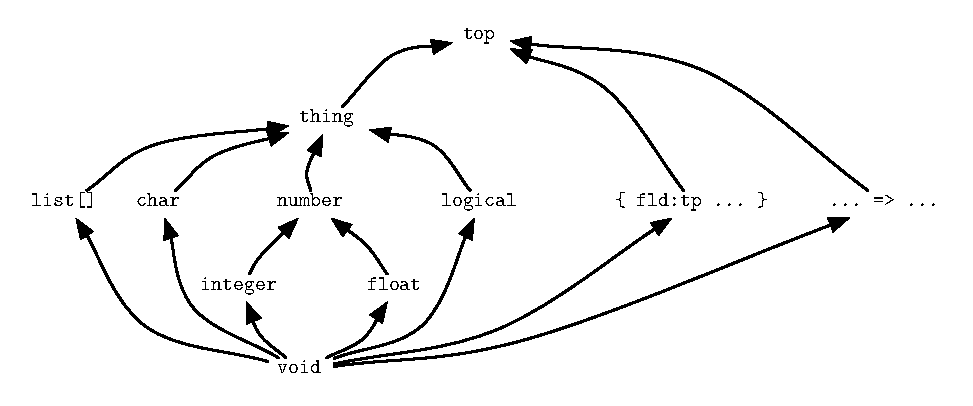
\includegraphics[width=\textwidth]{lattice}}
\caption{\label{type:lattice}Part of \go's standard type lattice}
\end{figure}

In the sub-type partial ordering, higher in the order means more general and lower in the ordering means more specific. Thus \q{top} type is the most general type (and therefore the least is known about values of type \q{top}) and \q{void} is so specific that there are \emph{no} legal \q{void} values.

The significance of \q{top} and \q{void} is largely technical, however, a function that accepts \q{top} arguments will accept anything and a \q{void} value is acceptable for all functions. On the whole, if you see either \q{top} or \q{void} in a type expression in an error message, you are likely to be in trouble!

You will notice that \go's type lattice is wide and shallow -- that for the most part there are few significant \firstterm{chain}{A chain is a sequence of types where for each pair of types in the link \emph{T\subi} and \emph{T\sub{i+1}} it  known that \emph{T\subi} is a subtype of \emph{T\sub{i+1}}. All types are in a chain of at least three elements: \q{void}, the type itself and \q{top}.}s in the lattice. This is in the nature of type lattice systems. However, when defining types, particularly in terms of type inheritance, then we do get a richer network. For example, figure~\vref{type:lattice:number} shows the lattice associated with the \q{number} type.

\begin{figure}
\centerline{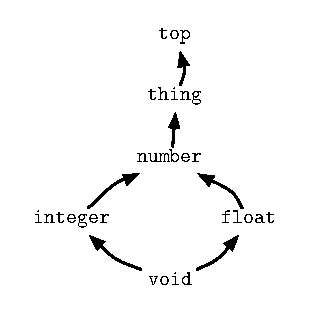
\includegraphics{numberlattice}}
\caption{\label{type:lattice:number}\go's \q{number} type lattice}
\end{figure}

This graph highlights the fact that a lattice is not necessarily a simple \firstterm{basket}{A basket type lattice is one where every chain is exactly three elements long; effectively meaning that there is no significant subtype relationship between non-trivial type elements.} or \emph{chain}, but can have have branching elements in it. It cannot, however, have cycles -- a lattice with a cycle is not permitted.

\subsection{Polymorphism}
Types  may be \firstterm{polymorphic}{A type that is not completely ground -- it may refer to many kinds of values.} and \firstterm{recursive}{A recursive type is one which may have components of the same type as the overall type.}. This polymorphism is reflected in the names of types -- they can have type arguments. For example, the \q{char} type is the type of characters; and \q{list[char]} represents the type list  of \q{char}acters -- i.e., \q{string}s.

The list type (\q{list[\emph{type}]}) is polymorphic: it requires a type argument which is the type of the elements of the list. It is also recursive because the type of a component element of a list term -- namely the tail of the list -- is also of the same type as the whole list.  A recursive type is one whose values contain components that are of the same type as the whole. Although the \q{list[\ldots]} type is built-in to \go, it is straightforward to define new recursive types. 

Recursive types have a particular hallmark: their type terms are \emph{opaque} -- it is not possible to infer solely from the type expression what values of that type look like. For example, although a list is necessarily defined as a term which includes a list as a component (the tail of a list is also a list of the same type) that recursion is not itself reflected in the \q{list} type term. In contrast with this, type expressions for functions are \emph{transparent} -- it is obvious from the type term what the structure of the values are -- and conversely, transparent types may not be recursive. For tuples, that means, for example, that it is not possible to define a tuple type in \go that has the same tuple type as itself as one of the elements of the tuple:
\begin{example}
\begin{boxed}
\begin{alltt}
( number, ( number, ( number, \ldots)))
\end{alltt}
\end{boxed}
\caption{\label{recursive:tuple}an impossible recursive tuple type}
\end{example}

\section{Standard Types}
\label{types:types}
\index{types}
\go has a range of built-in `atomic' types:  \q{integer}, \q{float}, \q{char} and \q{symbol}; and a range of built-in \emph{type constructors}:
\begin{itemize}
\item
\q{list[\emph{type}]} (list of \emph{type}), 
\item
\q{[\emph{type\sub1},\ldots,\emph{type\subn}]\{\}} (predicate type), 
\item
\q{[\emph{type\sub1},\ldots,\emph{type\subn}]=>}\emph{type} (function type), 
\item
\q{[\emph{type\sub1},\ldots,\emph{type\subn}]-->}\emph{type} (grammar type),
\item
\q{[\emph{type\sub1},\ldots,\emph{type\subn}]*} (action type), and
\item
\q{\{ \emph{field\sub1}:\emph{type\sub1}. \ldots \emph{field\subn}:\emph{type\subn}. \}} (type interface)
\end{itemize}

\subsection{Type variables}
\label{types:standard:variable}

\index{type variable}
\go does not use any special lexical markers to distinguish type variables from other variables, or even other type names -- the scope of the identifier serves to distinguish the cases. An identifier \q{foo} occurring in a type expression will refer to a type name if a type definition for \q{foo} is `in scope'; otherwise it refers to a type variable.

The normal scope rules do not apply for certain of \go's built-in types; for example, the identifier \q{number} (say) is predefined in the language and always refers to the \q{number} type.

\paragraph{Universally quantified types}
\index{unversally qunatified types}
\index{type variable!universal}
A \emph{universally} quantified type is written using the notation:
\begin{alltt}
[s\sub1,\ldots,s\subn]-\emph{Type}
\end{alltt}
this type binds the type variables s\subi{} occurring in the \emph{Type} expression. \go supports nested quantification of type terms: if \emph{Type} contains a type expression that is itself quantified and binds any or all of the \q{s\subi} type variables then the inner occurrences refer to the inner-most quantification.

It is not normally required to manually identify the type variables in a type expression in this way; however, when type expressions are printed (in error messages typically) they will be displayed in fully quantified form.


\subsection{Standard value types}
\label{types:standard}
\index{types!standard types}

Most of \go's standard types are defined in a standard library: \q{go.stdlib}. This library, which also includes a number of utility definitions, is automatically \q{import}ed in every package.\footnote{It is possible, if not advised, to suppress this behavior with a special compiler option.}

\subsubsection{\q{thing} type}
\label{types:standard:thing}

\index{thing@\q{thing} type}
\index{type!thing@\q{thing} type}

The \q{thing} type is the top of the value part of the type lattice -- all values are a sub-type of \q{thing}. It is not the top of the type lattice itself -- that is \q{top}. The program types -- such as function type -- are not a sub-type of \q{thing} -- although they are sub-types of \q{top}.

The \q{thing} type has a simple type interface; it is declared to be:
\begin{alltt}
thing \impl \{ 
  show:[]=>string.
  meta:[]=>meta.
  \}.
\end{alltt}
The \q{show} function is used to compute a printable \q{string} display of a term and \q{meta} is used to compute a meta-term representation of a term. Note that different types of terms may well use different methods for displaying themselves; it is only the \emph{type} of \q{show} that is defined at this juncture.
  

\subsubsection{\q{number} type}\
\label{types:standard:number}

\index{number@\q{number} type}
\index{type! number@\q{number} type}
The \q{number} type symbol is used to denote the union type of integer and floating point values and expressions. The \q{number} type has the definition:
\begin{alltt}
number \impl thing.
\end{alltt}

\subsubsection{\q{integer} type}
\label{types:standard:integer}

\index{integer@\q{integer} type}
\index{type!integer@\q{integer} type}
The \q{integer} type symbol is used to denote the type of integer values and expressions. The \q{integer} type has the definition:
\begin{alltt}
integer \impl number.
\end{alltt}

\subsubsection{\q{float} type}
\label{types:standard:float}

\index{float@\q{float} type}
\index{type! float@\q{float} type}
The \q{float} type symbol is used to denote the type of floating point values and expressions. The \q{float} type has the definition:
\begin{alltt}
float \impl number.
\end{alltt}

\begin{aside}
  Note that there is no subtype relationship between \q{integer}s and \q{float}s. They are, however, both subtypes of the standard type \q{number}.  This can occasional quirks where it is necessary to specifically convert \q{integer} values to \q{float}s using the built-in function \q{n2float}.
\end{aside}

\subsubsection{\q{char} type}
\label{types:standard:char}

\index{char@\q{char} type}
\index{type!char@\q{char} type}
The \q{char} type symbol is used to denote character values and expressions. The \q{char} type has the definition:
\begin{alltt}
char \impl thing.
\end{alltt}

\subsubsection{\q{symbol} type}
\label{types:standard:symbol}
\index{symbol@\q{symbol} type}
\index{type!symbol@\q{symbol} type}

The \q{symbol} type symbol is use to denote symbol values and expressions. Note that this type refers to the `general' class of symbols -- literals of which are written as identifiers surrounded by single quote characters. The other main class of symbols -- those introduced within user-defined type definitions are not covered by this type symbol; and nor are they written with single quotes.

The \q{symbol} type has the definition:
\begin{alltt}
symbol \impl thing.
\end{alltt}


\subsubsection{\q{logical} type}
\label{types:standard:logical}
\index{logical@\q{logical} type}
\index{type!logical@\q{logical} type}

The \q{logical} type is used to denote truth values. Although a standard type, \q{logical} can be defined as a normal user-defined type, using the type definition:
\begin{alltt}
logical ::= true | false.
\end{alltt}

\subsubsection{\q{opaque} type}
\label{types:standard:opaque}
\index{opaque@\q{opaque} type}
\index{type!opaque@\q{opaque} type}
The \q{opaque} type symbol is used to denote certain `internal' values that are managed by the \go system. There is no written notation that corresponds to opaque literal values, and they will never be displayed in normal circumstances.

\subsubsection{\q{meta} type}
\label{types:standard:meta}
\index{meta@\q{meta} type}
\index{type!meta@\q{meta} type}

The \q{meta} type is used to represent a meta-level representation of a term. It is defined using the definition:
\begin{alltt}
meta \impl thing.
\end{alltt}

\subsubsection{Tuple type}
\label{types:standard:tuple}
\index{tuple@\q{,} type}
\index{type!tuple@\q{,} type}

The \q{,} type is used to denote pairs of values. Although a standard type, \q{,} can be defined as though it were a normal user-defined type, using the definition:
\begin{alltt}
(u,v) ::= (u,v).
\end{alltt}
This rather bizarre type definition declares that the tuple type -- denoted by the type term \q{(u,v)} has a single constructor, also \q{(u,v)}. This notation is a slight twist on the normal type notation -- we are using the \q{,} operator as an infix type operator which is not actually permitted in programs.

\subsubsection{\q{list} type}
\label{types:standard:list}

The list type is used to denote lists of values. The list type is written using the notation:
\begin{alltt}
list[\emph{type}]
\end{alltt}
For example, the type expression:
\begin{alltt}
list[char]
\end{alltt}
denotes the type `list of \q{char}'. This is the type assignment given to expressions which are inferred to be lists of \q{char}acter -- including string literals. \go supports the \q{string} synonym for the \q{list[char]} type term.

The \q{list} type has a definition equivalent to:
\begin{alltt}
list[t] \impl thing.
list[t] \impl \{
    head:[]=>t.                -- head of the list
    tail:[]=>list[t].          -- tail of the list
    eof:[]\{\}.                  -- is the list empty
    cons:[t]=>list[t].         -- new list on the front
    tack:[t]=>list[t].         -- new list on the back
    hdtl:[t,list[t]]\{\}.        -- pick off the head and tail
    eq:[list[t]]\{\}.            -- is equal to this list
\}
\end{alltt}

\subsection{Program types}

\subsubsection{Type modes}
\index{type mode}

Program types have argument types that denote the types of arguments to the program. However, the types of arguments are also associated with \emph{modes} -- which express constraints on the flow of information into or out of a program via its arguments.

There are four kinds of modes: input mode, super-input mode, output mode and bidirectional mode:
\begin{description}
\item[input mode]
If an argument is marked as being input mode then the expectation is that data flows into the program through that argument. This carries two implications: one for type checking and one dynamic data flow:
\begin{itemize}
\item
An actual argument to a program that corresponds to an input moded argument may have a type that is a sub-type of the expected type.
\item
An actual argument to a program must not be \emph{bound} as a result of the matching of input arguments to patterns. Where the actual argument is a non-variable, this is not an issue; where the actual argument is an unbound variable then either the matching pattern also corresponds to an unbound variable or the match will \emph{fail}.
\item
In order to explicitly note an argument type to be input, suffix the type of the argument with the \q{+} operator:
\begin{alltt}
pp:[integer+]\{\}
\end{alltt}
\end{itemize}

\item[super input mode]
The super input mode is based on the input mode; with the additional operational characteristic that if a program is invoked where the super input moded argument is unbound then the call to the program is \emph{delayed} until such time as the variable becomes bound.

If the variable is never instantiated, then the delayed program is never invoked.

The super input mode is marked by suffixing the type of the argument with the \q{++} operator:
\begin{alltt}
listOfInt:[list[integer]++]\{\}
\end{alltt}

\item[output mode]
An output moded argument is the converse of an input moded argument:
\begin{itemize}
\item An actual argument's type must be \emph{equal} to the expected type for that program argument.
\item at run-time an actual argument \emph{must} be an unbound variable; otherwise the matching of patterns to values will \emph{fail} even if the corresponding pattern is an unbound variable.
\item
In order to explicitly note an argument type to be output, suffix the type of the argument with the \q{-} operator:
\begin{alltt}
pp:[integer-]\{\}
\end{alltt}
\end{itemize}

\item[bidirectional mode]
A bidirectional moded argument can be either input or output; and unification is used to match the actual argument to the pattern.
\begin{itemize}
\item
The type of the actual argument must be equal to the expected type for that argument
\item
Unification is used to match the incoming value against the pattern; hence the flow of information may be either incoming, outgoing or a mixture.
\item
In order to explicitly note an argument type to be bidirectional, suffix the type of the argument with the \q{-+} operator:
\begin{alltt}
pp:[integer-+]\{\}
\end{alltt}
\end{itemize}
\end{description}

Although it is possible to associate modes with every argument type of every program type, program types have defaults that are intended to represent the normal mode of use for that kind of program.

\subsubsection{Function type}
\label{types:standard:function}

The function type is used to denote function values. The function type is written:
\begin{alltt}
[\emph{T\sub{1}},\ldots,\emph{T\sub{n}}] \funarrow{} \emph{T\sub{R}}
\end{alltt}
where \q{[\emph{T\sub{1}},\ldots,\emph{T\sub{n}}]} is a list of the type expressions corresponding to the arguments of the function and \emph{T\sub{R}} corresponds to the result of the function. For example, the type expression:
\begin{alltt}
[list[char],list[char]]=>list[char]
\end{alltt}
denotes a function -- from two string arguments to a string result.

The default mode for function arguments is \emph{input}. However, it is occasionally useful to mark a function argument as output -- as an out-of-band way of returning values from a function.

\subsubsection{Predicate type}
\label{types:standard:predicate}

The predicate type is used to denote relational or predicate values. The predicate type is written:
\begin{alltt}
[\emph{T\sub{1}},\ldots,\emph{T\sub{n}}]\{\}
\end{alltt}
where \q{[\emph{T\sub{1}},\ldots,\emph{T\sub{n}}]} is the list of type expressions of the arguments of the predicate. For example, the type expression:
\begin{alltt}
[list[char],list[char],list[char]]\{\}
\end{alltt}
denotes the type of a ternary predicate where all the arguments are strings.

The default mode for predicate arguments is \emph{bidirectional}. However, it is often useful to mark a predicate argument as input -- to be explicit about the expect usage of the predicate.


\subsubsection{Action type}
\label{types:standard:action}

The action type is used to denote procedure values. The action type is written using a postfix \q{*} operator:
\begin{alltt}
[\emph{T\sub{1}},\ldots,\emph{T\sub{n}}]*
\end{alltt}
where \q{[\emph{T\sub{1}},\ldots,\emph{T\sub{n}}]} is the list of type expressions of the arguments of the procedure. For example, the type expression:
\begin{alltt}
[list[char]]*
\end{alltt}
denotes the type of a unary procedure whose single argument is a string.

The default mode for action procedure arguments is \emph{input}. However, it is occasionally useful to mark an argument as output -- as that is the only way of arranging for output from an action procedure call.

\subsubsection{Grammar type}
\label{types:standard:grammar}

The grammar type is used to denote grammar values. The grammar type is written as a \q{-->} mapping from the types of the arguments of the grammar to the type of the stream of values the grammar is defined over:
\begin{alltt}
[\emph{T\sub{1}},\ldots,\emph{T\sub{n}}] --> \emph{T\sub{S}}
\end{alltt}
where \q{[\emph{T\sub{1}},\ldots,\emph{T\sub{n}}]} is the list of type expressions of the arguments of the grammar and \emph{T\sub{S}} is the type of the stream that the grammar is defined over -- typically a list of some kind. For example, the type expression:
\begin{alltt}
[number]-->list[char]
\end{alltt}
denotes the type of a grammar whose single argument is a number and which may be used to parse strings.

The default mode for grammar arguments is \emph{bidirectional}. However, it is occasionally useful to mark a grammar argument as input -- to be explicit about the expect usage of the grammar, and also to mark an argument as output -- to be explicit about the outputs associated with parsing a stream.

\subsubsection{Class type}
\label{types:standard:class}

\index{type!class}
\index{class type}
\index{type!@= type operator}
There are two kinds of class type declarations: those that introduce a stateless class and those that introduce a stateful class.

The state-free class type is used to denote constructor classes, analogous to constructor functions. The stateful class type denotes classes that may carry state.


A state-free class type declaration takes the form:
\begin{alltt}
\emph{class}:[\emph{T\sub1},\ldots,\emph{T\subn}] @= \emph{Type}.
\end{alltt}
The only permitted mode for the label arguments of a state-free class label is \emph{bidrectional}.

A stateful class type declaration takes the form:
\begin{alltt}
\emph{class}:[\emph{T\sub1},\ldots,\emph{T\subn}] @> \emph{Type}.
\end{alltt}
The default mode for label arguments of a stateful class label is \emph{input}.

\begin{aside}
The reason that state-free label arguments must be bi-directional is that class labels are equivalent to constructor functions: i.e., they have an inverse. That means that it is always possible to recover the arguments of a 'call' to a constructor function.

On the other hand, one of the differences between state-free class labels and statefull class labels is that the latter \emph{do not} have inverses -- they are semantically closer to regular functions.
\end{aside}
Note that a class type statement does not define the class itself, it simply defines its type.

\section{Algebraic type definitions}
\label{type:algebraic}

In addition to a type being defined using the sub-type statements, a type may also be introduced using an \emph{algebraic type definition} statement. An algebraic type definition is one where the type is introduced at the same time as a set of enumerated symbols and constructors for the type:
\begin{alltt}
\emph{UserT}[\emph{T}\sub1,\dots,\emph{T}\subn] ::= \dots\ | \emph{S} | \dots.
\end{alltt}
where \emph{T\subi} are identifiers indicating type arguments and the right hand side is a series of enumerated symbols and constructor function templates.

For example, the \q{tree} type defined below may be used to denote tree values:

\begin{alltt}
tree[a] ::= empty | node(tree[a],a,tree[a]).
\end{alltt}
This statement defines a new type type constructor \q{tree} together with the enumerated symbols and constructor terms that make up values of the \q{tree} type.

\subsection{Type parameters of a type definition}
\label{type:parameter}

Where the template of a \emph{UserType} takes the form:
\begin{alltt}
\emph{UserType}[\emph{T}\sub1,\dots,\emph{T}\subn] \impl \ldots
\end{alltt}
the various arguments \emph{T\subi} are the \emph{type parameter}s of the type definition. They must all be identifiers and they are interpreted as type variables. Such a \emph{UserType} is implicitly universally quantified with respect to the type parameters (hence the polymorphism of the type).

\go imposes a restriction on type variables occurring in a type definition: all type variables appearing in the body of the type definition -- i.e., appearing in templates for the type constructors in class definitions -- must also appear in the type template expression itself.

\subsection{Enumerated symbol}
\label{type:user-symbol}
An \emph{enumerated} symbol is equivalent to a zero-arity label term. For example, the introduction of \q{empty} in the definition of \q{tree} above is equivalent to the class definition:
\begin{alltt}
empty:tree[a] .. \{\}.
\end{alltt}

The type analysis of a definition of an enumerated symbol may be captured via an `introduced' type inference rule:
\begin{equation*}
\forall \vec{V}.\left\{\frac{}
{\typeprd{E}{\q{S}}{\q{\emph{UserT}[\emph{T}\sub1,\dots,\emph{T}\subn]}}}\right\}
\end{equation*}
where $\vec{V}$ are all the type variables ocurring in the type definition and \q{S} is the newly introduced enumerated symbol.

Note that, in general, the type of a enumerated symbol can have type variables even when clearly the symbol itself has no variables. We can see this more clearly with the empty list case. \go's list notation is based on the \q{,..} constructor function and the \q{[]} enumerated symbol; which might be captured in the algebraic type definition:
\begin{alltt}
list[T] ::= [T,..list[T]] | []
\end{alltt}
The type of an occurrence of the empty list is, then, an expression of the form:
\begin{alltt}
list[T\sub{i}]
\end{alltt}
where \q{T\sub{i}} may or may not be known. The logic of this is that an empty list is always of a list of a specific type -- even if we cannot determine what that type is in given circumstances.

\subsection{Constructor functions}
\label{type:constructor}
\index{contructor function definition}
\index{functions!constructor}

Constructor functions (a.k.a. class labels) are analogous to functors in \prolog: they fulfill very similar roles. However, their semantics are quite distinct to normal \prolog terms since they always are associated with logical theories -- even when defined within an algebraice type definition.

\begin{aside}
  Constructor functions are so-named because they are functions: with the
  particular property that every expression involving the constructor function
  has an exact inverse. This property allows constructor functions to be used as
  patterns as well as in other expressions.
\end{aside}

The type assignment for constructor functions can be viewed as an additional type inference rule; where a type definition was of the form:
\begin{alltt}
\emph{Template} ::= \ldots | \emph{F}(\emph{T\sub1},\ldots,\emph{T\subn}) | \ldots
\end{alltt}
we introduce a new inference rule of the form:
\begin{equation}
\LeftLabel{$\forall \vec{V}$}
\AxiomC{\typeprd{{\emph{E}}}{A\sub1}{\emph{T\sub{1}}}}
\AxiomC{\ldots}
\AxiomC{\typeprd{{\emph{E}}}{A\subn}{\emph{T\sub{n}}}}
\TrinaryInfC{\typeprd{{\emph{E}}}{\q{\emph{F}(\emph{A\sub1},\ldots,\emph{A\subn})}}
{\q{\emph{Template}}}}
\DisplayProof
\end{equation}
where $\vec{V}$ are the type variables ocurring in the type definition.

\subsection{Type extension}
One of the key features of \go's type system is its extensibility. In particular, because types are distinct from classes, there is always the potential to introduce new constructors for a type -- including types that have been introduced using an algebraic type definition.

For example, given the \q{tree[]} type, we may decide that we need a new kind of node for a tree -- perhaps a binary tree node that does not include a label. We can do so simply by defining a class for it:
\begin{alltt}
bin:[tree[a],tree[a]]@=tree[a].
bin(L,R) .. \{ \ldots \}
\end{alltt}
The effect of this is as though the original type definition were:
\begin{alltt}
tree[a] ::= empty 
        | node(tree[a],a,tree[a])
        | bin(tree[a],tree[a]).
\end{alltt}
We can even introduce this class in a different package than the one in which \q{tree[]} itself is defined:
\begin{alltt}
foo\{
  import tree.
  bin:[tree[a],tree[a]]@=tree[a].
  bin(L,R) .. \{ \ldots \}
\}
\end{alltt}
  


\chapter{Functions and Expressions}
\label{expressions}

This chapter is about the functional programming aspect of \go. \go has a rich range of expressions, one of its distinguishing characteristics when compared to \prolog. Part of this comes from the fact that \go combines a functional programming notation, and part comes from \go's multi-paradigm style: so there are expressions that relate expressions to actions and predicates as well as regular evaluable forms.

\section{Functions}
\label{expression:functions}
\index{functions}
\index{equations}

Functions are defined using sequences of equations. For example, Program~\vref{function:append} shows how a list concatenation function may be written. Each equation is a \emph{rewrite} equation that shows how to rewrite terms of one form -- representing the function call -- to terms of another form -- representing the value.
\begin{program}
\begin{boxed}
\begin{alltt}
concat:[list[T],list[T]]=>list[T].
concat([],X) => X.
concat([E,..X],Y) => [E,.. concat(X,Y)].
\end{alltt}
\end{boxed}
\caption{\label{function:append}A list \q{concat}enation function}
\end{program}
The type declaration says that \q{concat} is polymorphic, mapping a pair of lists of any type of element \q{T} to a list of elements of the same type.

Functions may be defined either within a class body -- in which case they are specific to that class -- or at the outer level of a package -- in which case they are global to the package. In both cases all the equations for a given function must be grouped together.

The general form of an equation is:
\begin{alltt}
\emph{Fun}(\emph{Ptn\sub1},\ldots,\emph{Ptn\subn} :: \emph{Condition} => \emph{Exp}
\end{alltt}
The equations in a function are applied in a left-to-right order. There is no deep backtracking in function evaluation: once an equation has been found that matches then no other equations will be attempted. In the event that none of the equations match an error exception
\begin{alltt}
error(\ldots,'eFAIL')
\end{alltt}
will be raised.

\paragraph{Matching equations to arguments}
\label{expression:equation:matching}
\index{equation!argument matching}
\index{argument matching in equations}
Note that, by default, the head arguments of an equation are \emph{matched} against the tuple of arguments rather than \emph{unified}. The distinction is that matching is not permitted to side-effect its input -- in this case matching against the head of an equation \emph{will not} side-effect the arguments to the function call.
For example, given a function application:
\begin{alltt}
F(X,2)
\end{alltt}
then if \q{F} is defined by the equation:
\begin{alltt}
F('a',2) => 3
\end{alltt}
then the match will \emph{fail} (and raise an error if there are no alternatives equations for \q{F}) since the only way that it could succeed would be by binding \q{X} to \q{'a'}. 

\begin{aside}
The only exceptions to this matching semantics are where the argument's mode as declared in the function's type declaration is bidirectional -- in which case the incoming argument will be \emph{unified} -- or if the argument is marked as output -- in which case the incoming argument must be an unbound variable and a value will be returned in that argument.

For example, the type declaration:
\begin{alltt}
F:[symbol-,integer]=>integer.
\end{alltt}
would require the above equation for \q{F} to be applied to a function call in which the first argument was unbound, and would permit equations that define \q{F} to instantiate the argument. 
\end{aside}

\begin{aside}
\index{match predicate}
\index{\q{.=} predicate}
The match predicate \q{.=} (see Section~\vref{goal:match}) may be used within a guarded term to achieve a similar matching semantics as for the head arguments themselves.
\end{aside}

The type inference rule for the equations defining a function \q{F} is:
\index{type inference!equation}
\begin{equation}
\AxiomC{\typeprd{\emph{E}}{\q{\emph{F}}}{\q{\emph{F\sub{H}}=>\emph{F\sub{R}}}}}
\AxiomC{{F\sub{H}}={T\sub{H}}}
\AxiomC{\subtype{F\sub{R}}{T\sub{R}}}
\TrinaryInfC{\typesafe{\emph{E'}}{\q{\emph{H}::\emph{G}=>\emph{R}}}}
\DisplayProof
\end{equation}
I.e., the main requirement for a safe equation is that the head arguments have the same types as the declared argument types and the type of the right hand side expression of the equation is less than or equal to the function result type.

\begin{aside}
Note that the type rule for an equation is independent of the modes associated with the function type. In all cases, the type of the argument pattern must be the same as the type of the function. Modes affect calls to functions, and hence the right hand sides of equations, but do not affect the type analysis of argument \emph{patterns}.
\end{aside}

\section{Atomic expressions}
\label{expression:atomic}

The atomic \go expressions are the atomic or unstructured elements of the language: including characters, symbols and numbers. They are called atomic because, from the \go programmer's perspective, they have no internal structure. 

\subsection{Symbols}
\label{expression:symbol}

\index{expression!symbols}
\index{symbol literal expression}
As outlined in Section~\vref{token:symbol}, a symbol is written as a sequence of characters enclosed in single quotes. Symbols are one of the primitive data types of \go, and have the type \type{symbol}.

We define the type inference rule for symbols thus:
\index{type inference!symbol}
\begin{equation}
\frac{}
{\typeprd{E}{\q{'\emph{S}'}}\q{symbol}}
\end{equation}
which is interpreted as
\begin{quote}
The type of an expression of the form \q{'\emph{S}'} is \q{symbol}.
\end{quote}

Logically, a symbol is a token that identifies an individual entity in the modeled world. \go supports other kinds of symbols than quoted \q{symbol}s; user defined symbols as introduced via class definitions or in algebraic type definitions do not carry the \q{symbol} type: their type is that of the declared type. Such symbols are written using the normal identifier notation.

\subsection{Characters}
\label{expression:character}

\index{expression!character}
\index{character expression}
A character literal is written as a back-tick character followed by the character itself; which may be a string character reference. Characters are one of the core data types of \go: lists of \q{char}acters form the basis of \go's string notation.

The type of a character expression is \q{char}:
\index{type inference!character}
\begin{equation}
\frac{}
{\typeprd{E}{\q{`\emph{C}}}\q{char}}
\end{equation}


\subsection{Numbers}
\label{expression:number}
%klc mostly copied from Lets Go!
\index{expression!number}
\index{number@\q{number} expression}
\go partitions numbers into two categories: \q{integer}s and \q{float}ing point numbers. Both of these are sub-types of the \q{number} type; however, neither \q{integer} nor \q{float} are sub-types of each other. This reflects the common reality that integral and non-integral \q{number} values are represented differently.

There are various ways of writing integer literals: as decimal integers, hexadecimal numbers and character codes.

\subsubsection{Integers}
\index{integer}
An integer is written as a sequence of decimal digit characters -- with an optional leading minus sign to denote negative integers. Although the standard ASCII digit characters are likely to be the most common digit characters used, there are approximately 250 decimal digit characters in the Unicode standard! The \go parser supports the use of any Unicode decimal digit characters in constructing a number; however, the \go system only uses ASCII digits when displaying numbers.

\paragraph{Hexadecimal numbers}
\index{integer!hexadecimal}
A hexadecimal number is written with a leading \q{0x} followed by hexadecimal digits. Note that, unlike regular integers, \go requires that hexadecimal numbers use only the ASCII digit characters, together with upper-case or lower-case letters \q{A} to \q{F}.

\begin{alltt}
0xffff 0xabd 0x0
\end{alltt}
are all integers, of type \q{integer}, written using hexadecimal notation.

\paragraph{Character codes}
\index{integer!character code}
\index{Unicode!character code}
It is also possible to specify an integer as the Unicode code value of a character. Such an \q{integer} is written with a leading \q{0c} followed by a single character reference. Thus, for example, the literal:
\begin{alltt}
0cA
\end{alltt}
is the number 65 -- as the Unicode code point value associated with upper-case \q{A} is 65. Similarly, \q{0c\bsl{}n} is the \q{integer} 10, as the character \q{\bsl{}n} refers to the new-line character -- whose code value is 10. The value of
\begin{alltt}
0c\bsl{}+2334;
\end{alltt}
is, of course, the same as:
\begin{alltt}
0x2334
\end{alltt}

\index{type inference!integer}
\begin{equation}
\frac{X \mbox{ is an integer literal}}
{\typeprd{E}{X}{\q{integer}}}
\end{equation}

\subsubsection{Floating point numbers}
\index{floating point}
\index{number!floating point}
\go distinguishes floating point numbers from integral values by the fact that floating point numbers always have a decimal point: i.e., a floating point number is written as a fractional number followed by a fractional part and an optional exponent expression. Example floating point numbers include:
\begin{alltt}
34.56 2.0e45 2.04E-99
\end{alltt}
Since the period character has so many uses in \go, there are some special rules for them. In the case of a floating point number there may be no spaces on either side of the period; i.e., the program text:
\begin{alltt}
34 . 23
\end{alltt}
does \emph{not} denote the number 34.23; it is three tokens: the integer 34, the rule terminator \q{\dotspace} and the integer 23.

Floating point literals are of type \q{float}, a sub-type of \q{number}.
\index{type inference!float}
\begin{equation}
\frac{X \mbox{ is a float literal}}
{\typeprd{E}{X}{\q{float}}}
\end{equation}

\section{Variables}
\label{expression:variable}

\index{expression!variable}
\index{variable expression}
Variables are written as identifiers (see Section \vref{token:identifier}). All identifiers which have not been defined as class labels or names of rule programs or declared as enumerated symbols or constructor functions in an algebraic type definition are considered to be variables. \go does not have a variable convention to distinguish variables; instead we use the context of the identifier to distinguish them. Note that normal symbols (see Section~\vref{expression:symbol}) are always surrounded by single quotes and cannot be confused with variables.

\index{type inference!variable}
All variables have types, and each occurrence of a variable is type-checked -- resulting in type constraints on its type: the constraints inferred with respect to each occurrence of a must be consistent.  

A variable may not have a value and yet still have a type associated with it.

\subsection{Scope of identifiers}
\label{variable:scope}

\index{variable!scope}
\index{identifier!scope}
\index{scope of identifiers}
\go does not require that variables in rules be explicitly introduced -- simply, an identifier occurring in a pattern or expression that does not have a prior declaration is assumed to be a variable. However, there are rules that define the \emph{scope} of a variable: i.e., the textual range across which occurrences of the same name are considered to refer to the same variable.

For identifiers such as program names, type names and class names, introduced in the body of a class or package, they are in scope across the entire class body or package -- there is no implied scope arising from the order of declarations. For variables in rules, the scope of the variable is the entire rule. Similarly, program names are in scope for their entire enclosing context, regardless of the order of declaration.

For a rule, such as an equation or a clause, any variables mentioned in the rule that are not defined in an outer scope -- either in an enclosing class body or as package variables -- are local to that rule.

A variable is \emph{free} in a rule if its scope encompasses the rule as well as other, enclosing, program fragments. The main source of free variables in a rule are \emph{label variables} of the class in which the rule is embedded. For example, in:
\begin{alltt}
lbl(X)..\{
  bar(X) :- X<10.
\}
\end{alltt}
the variable \q{X} is \emph{free} in the \q{bar} clause. The reason is that \q{X} is also a variable occurring in the label \q{lbl(X)} of the class that the \q{bar} clause is embedded.


\paragraph{Holes in the scope}
\index{variable!scope!holes in}
\index{identifier!scope!holes in}
A hole in the scope of an identifier  -- i.e., where an inner use of an identifier can `hide' an outer identifier with the same name -- can occur when the inner use of the identifier is as the name of a defined program of a class body.  The inner variable masks out, throughout its natural scope,  any variable of the same name defined in outer contexts. 

Note that variable identifiers in rules \emph{do not} mask out variables of the same name in outer scopes.  Such a variable is a \emph{free} variable of the rule. This is the principal mechanism in many cases whereby a program is referenced in function and predicate calls in the bodies of rules.

Consider the following definition of the state-free class:
\begin{alltt}
funny:[T\sub1,T\sub2,T\sub3] @= aType.
funny(A,Y,B)..\{
  A(X).
  A([X,..Y]) :- B.is(X),A(Y).
\};
\end{alltt}
The variable \q{B} introduced in the \q{funny} constructor is in scope across the whole of the class body defining \q{funny}. It is therefore a global variable of this class. 

The variable \q{A} is in scope throughout the class as well. However, there is a definition of \q{A} in the class body that uses the same name \q{A}; this definition masks out the \q{A} that occurs as a parameter of the \q{funny} constructor.  In effect, the \q{funny} class cannot use its \q{A} argument as it is masked by the inner \q{A} definition in the class body.

The \q{X} variable has two `incarnations': in the first clause of the definition of \q{A} and in the second clause. These are separate variables. The \q{X} of the first clause is local to that clause.

The \q{Y} variable occurring in the head of second clause of \q{A} is \emph{not} local -- it is bound by an outer occurrence of the same variable in the argument list of the \q{funny} constructor. Like the \q{B} variable in the same clause, it is a \emph{free} variable of the \q{A} program.

\paragraph{Singleton variables}
\index{variable!singleton occurrence}
Note that the compiler will report a warning over any \emph{singleton} occurrences of variables -- unless the variable has a leading underscore in its name. Such singleton variables are often actually misspelt variables -- hence the warning from the compiler. In this case, the compiler would report a warning over both the \q{A} parameter of the function and the \q{X} parameter of the first \q{A} clause. The former helping to highlight the fact that \q{A} is effectively masked out by the theta environment.

\subsubsection{Scope of type variables}
\index{scope!of type variables}
\index{type variables!scope of}
Like regular variables, type variables also have an associated textual scope. The scope rules for type variables are essentially the same as for normal identifiers. Of particular interest are type variables occurring within rules that are \emph{not} free -- i.e., are not mentioned in an outer context. Such type variables have the same scope as a regular variable: the rule in which the variable is mentioned.

\section{Standard structured terms}
\label{expression:structured}

\index{structured terms}
\go has two standard data constructor types: lists and tuples. In addition, of course, it is possible to define additional data constructors using class definitions and algebraic type definitions.

\begin{aside}
In fact, both lists and tuples are definable using normal \go mechanisms for defining constructor terms. They are highlighted because of their special role in the language.
\end{aside}

\subsection{Lists}
\label{expression:lists}

\index{list expression}
\index{expression!lists}
Lists are a standard data type of \go, the list data type is described in detail in Section~\vref{types:standard:list}. The surface syntax of lists is defined in Section~\vref{grammar:lists}. 

A list is a sequence of values. The defining characteristic of a list is that the first element of the list -- called  the \emph{head} of the list -- and the remaining sequence of elements after the head -- called the \emph{tail} of the list -- are available in a single constant step of computation. This distinguishes lists from arrays -- where every element is available in constant time although arrays are not easily extended -- and sets where each element may take $\log{}(n)$ time to access and there is only one occurrence of each element.

Lists are written as a sequence of comma-separated expressions enclosed in square brackets. For example, the list
\begin{alltt}
[1,2,3]
\end{alltt}
is a list of three \q{number}s: 1, 2 and 3, as is the expression:
\begin{alltt}
[1,1+1,1+1+1]
\end{alltt}

\paragraph{List pattern notation}
\index{lists!pattern}
There are two standard constructors for the list type: the empty list -- written as \q{[]} -- and the list cons constructor -- written as the special infix operator \q{,..} consisting of a head element and a tail list:
\begin{alltt}
[\emph{H},..\emph{T}]
\end{alltt}
There is a direct correspondence between list patterns and list terms: the expression:
\begin{alltt}
[1,[2,[3,..[]]]
\end{alltt}
is equivalent to the list \q{[1,2,3]}.

Other forms of list pattern are also interesting. For example, the list pattern:
\begin{alltt}
[1,2,3,..X]
\end{alltt}
denotes a list whose first three elements are known but whose tail is represented by the variable \q{X}. It is one of the magic aspects of logic programming that unifying \q{X} with \q{[4,5]} say, will have the effect of completing the above list pattern to
\begin{alltt}
[1,2,3,4,5]
\end{alltt}


The type rules for the standard list constructors are 
\index{type inference!lists}
\begin{equation}
\label{emptylist:type}
\AxiomC{}
\UnaryInfC{$\forall T.\typeprd{E}{\q{[]}}{\q{list[\emph{T}]}}$}
\DisplayProof
\end{equation}
and
\begin{equation}
\label{nonempty:type}
\AxiomC{\typeprd{E}{\q{H}}{T\sub{t}}}
\AxiomC{\typeprd{E}{\q{T}}{\q{list[{T\sub{t}}]}}}
\BinaryInfC{\typeprd{E}{\q{[H,..T]}}{\q{list[{T\sub{t}}]}}}
\DisplayProof
\end{equation}

\noindent
\index{type inference!complex expressions}
We can concatenate type inference rules to infer the types of more complex expressions. For example, we can use the type inference rules \ref{emptylist:type} and \ref{nonempty:type} to derive the type of this expression:
\begin{alltt}
[1,2]
\end{alltt}
which gives the type derivation:
\begin{prooftree}
\AxiomC{}
\UnaryInfC{\typeprd{E}{\q{1}}{\q{number}}}
\AxiomC{\typeprd{E}{\q{2}}{\q{number}}}
\AxiomC{\typeprd{E}{\q{[]}}{\q{list[T]}}}
\BinaryInfC{\typeprd{E}{\q{[2]}}{\q{list[number]}}}
\BinaryInfC{\typeprd{E}{\q{[1,2]}}{\q{list[number]}}}
\end{prooftree}



\subsection{Strings}
\label{expression:string}
\index{expression!strings}
\index{strings!lists of characters}
\index{lists of characters are strings}
\go string literal values are synonyms for lists of \q{char}s; i.e., a string literal such as \q{"foo"} is equivalent to the list:
\begin{alltt}
[`f,`o,`o]
\end{alltt}
and the empty string \q{""} is equivalent to
\begin{alltt}
[]:list[char]
\end{alltt}
i.e., an empty list with the added type annotation that it's type is list of \q{char}s (see Section~\vref{expression:typeannotation}).

\subsection{Tuples}
\label{expression:tuples}

\index{expression!tuple}
\index{tuple epxressions}
Like lists, tuples represent a way of aggregating values in a sequence. A tuple is written as a sequence of elements, separated by \q{,} and enclosed in parentheses:
\begin{alltt}
\label{foo:bar:tuple}('foo',23,['bar'])
\end{alltt}
Unlike lists, the elements of a tuple do not need to be of the same type. 

As used in a tuple, the comma (\q{,}) is an infix constructor operator.  The tuple type is provided as a convenient way of grouping values together; but it has no interface per se. The tuple type is defined as though by the type definition:
\begin{alltt}
(,)[s,t] ::= (s,t)
\end{alltt}
where \q{s} and \q{t} represent the two degrees of polymorphic freedom available in a tuple.

This, rather circular, definition highlights the fact that, in \go, the \q{,} infix operator is used both as the name of the tupling type as well as the tupling operator itself. It is, however, semantically, simply a predefined type with a single constructor that is very similar to a user-defined type.

The \q{,} operator is right associative, so it is possible to combine it into longer sequences:
\begin{alltt}
('joe',23,"his place",tonight)
\end{alltt}
is equivalent to:
\begin{alltt}
('joe',(23,("his place",tonight)))
\end{alltt}

\subsection{Function Call Expression}
\label{expression:applicative}

\index{applicative expressions}
\index{function!call expression}
\index{expression!applicative}
A function call is an expression of the form:
\begin{alltt}
\emph{Fun}(\emph{A\sub1},\ldots,\emph{A\subn})
\end{alltt}

\index{type inference!applicative expression}
Function call expressions are typed using a rule that maps the type of the function and the type of the argument to the type of the result. Assuming a normal mode assignment for the type of a function \q{F}, the type rule for a function application is:
\begin{equation}
\label{expression:applictype}
\AxiomC{\typeprd{E}{F}{\vec{L}\funarrow{}R}}
\AxiomC{\typeprd{E}{\vec{A}}{\vec{A\sub{t}}}}
\AxiomC{\subtype{$\vec{A\sub{t}}$}{$\vec{L}$}}
\TrinaryInfC{\typeprd{E}{\q{F($\vec{A}$)}}{R}}
\DisplayProof
\end{equation}

If there is one or more bidirectional or output moded arguments associated the function then the condition:
\[
\subtype{$\vec{A\sub{t}}$}{$\vec{L}$}
\]
becomes type equality:
\[
{\vec{A\sub{t}}}={\vec{L}}
\]
For constructor functions, type equality is also required.

Note that if an applied function fails, if none of the function's equations apply to the arguments of the application, then an \q{'eFAIL'} error exception is raised. This may be caught using an \q{onerror} clause.

\section{Special expressions}
\label{expression:special}

There are a number of expressions which are syntactic in nature, these include guarded expressions, action expressions, type annotated expressions and expressions relating to attribute sets.


\subsection{Type annotation}
\label{expression:typeannotation}
\index{type!annotation}
A \firstterm{type annotated expression}{An expression whose type is explicitly marked by the programmer.}  takes the form:
\begin{alltt}
\emph{Ex}:\emph{Type}
\end{alltt}
A type annotated expression has the same value as its non-annotated component. The only effect of the type annotation is to add a type constraint to the expression:
\begin{equation}
\frac{\typeprd{E}{\emph{Ex}}{\emph{Type}}}
{\typeprd{E}{\emph{Ex{\tt:}Type}}{\emph{Type}}}
\end{equation}
Type annotations are only rarely required within a normal \go program. However, they can serve as useful documentation and in those circumstances where there is a hard to track down type error.

\subsection{Bag of expression}
\label{expression:bagof}

The \firstterm{bag of}{A list-valued expression whose value is determined by finding all solutions to a predicate condition.} a list,  expression is a `cousin' of the guarded expression -- instead of a single expression which is defined if a goal is satisfied, a bag of expression represents the list of all the possible answers to a question. The bag of expression is written:
\begin{alltt}
\{ \emph{Ex} || \emph{Goal} \}
\end{alltt}
The value of a bag of expression is a list consisting of a copy of the value of \emph{Ex} for each way that \emph{Goal} can be satisfied. The order of elements in the resulting list is the same as the order that \emph{Goal} gives rise to possible solutions. It is of course possible for there to be multiple occurrences of a given value (hence the term `bag of').

The type inference rule for the bag of expression is:
\begin{equation}
\AxiomC{\typeprd{\emph{E}}{\emph{Ex}}{\emph{T\sub{Ex}}}}
\AxiomC{\safegoal{\emph{E}}{\emph{Goal}}}
\BinaryInfC{\typeprd{\emph{E}}{\q{\{\emph{Ex}||\emph{Goal}\}}}{\q{list[}\emph{T\sub{Ex}\q{]}}}}
\DisplayProof
\end{equation}

\paragraph{Variables in bags}
may arise when \emph{Ex} is not completely ground for one or more solutions to \emph{Goal}. The list returned will also contain variables. More precisely, the bag-of algorithm works as follows:
\begin{enumerate}
\item
The \emph{Goal} is evaluated. If no solution to \emph{Goal} is possible, then the value of \q{\{\emph{Ex}||\emph{Goal}\}} is the empty list.
\item
Each time a solution to \emph{Goal} is found, a `frozen copy' of \emph{Ex} is computed -- in the context of the solution to \emph{Goal}. This involves taking copies of any variables in \emph{Ex} to produce new variables.

After the \emph{Ex} value is computed, a failure is forced to attempt to find additional solutions to \emph{Goal}.
\item
After the last solution to \emph{Goal} has been found, the list of solutions found is `thawed' and returned as the value of the bag expression.
\end{enumerate}

\subsection{Bounded set expression}
\label{expression:bounded}

The \firstterm{bounded set}{A list valued expression whose value is determined by applying a predicate test to all elements of a base list.} expression is similar in form, and in some cases similar in use, to the \emph{bag of} expression (see Section~\vref{expression:bagof}). However, it owes its origin to a different style of programming and has quite different semantics.

The general form of the bounded set expression is:
\begin{alltt}
\{ \emph{Ex} .. \emph{Ptn} in \emph{List} \}
\end{alltt}
The value of a bounded set expression is a list consisting of evaluating the expression \emph{Ex} for each member of \emph{List} that matches with \emph{Ptn}.

The semantics of the bounded set expression can be given in terms of a defining mapping from such expressions into other \go expressions. I.e., a bounded set expression is entirely equivalent to the expanded form:
\begin{alltt}
bounded\sub{X}(\emph{List},\emph{Free})
\end{alltt}
where \q{bounded\sub{X}} is a new identifier not occurring anywhere else and is defined as though by the program:
\begin{alltt}
bounded\sub{X}([],\emph{Free}) => [].
bounded\sub{X}([\emph{Ptn},..L],\emph{Free}) => [\emph{Ex},..bounded\sub{X}(L,\emph{Free})].
bounded\sub{X}([_,..L],\emph{Free}) => bounded\sub{X}(L,\emph{Free}).
\end{alltt}
where \emph{Free} is the tuple of free variables in \emph{Ptn} and \emph{Ex}. I.e., a bounded set is evaluated by a recursive iteration through the elements of the bounding set, computing an output value for each succesful match of the list element. 

Note that the \emph{Ptn} pattern may have a guard associated with it, considerably increasing the potential power of the form. For example, 
\begin{alltt}
\{ X*X .. (X::X<10) in [1,2,3,50,23,2] \}
\end{alltt}
will return the list:
\begin{alltt}
[1,4,9,4]
\end{alltt}

The type inference rule for the bounded set expression is:
\begin{equation}
\AxiomC{\typeprd{\emph{E}}{\emph{Ex}}{\emph{T\sub{x}}}}
\AxiomC{\typeprd{\emph{E}}{\emph{Ptn}}{\emph{T\sub{S}}}}
\AxiomC{\typeprd{\emph{E}}{\emph{List}}{\q{list[\emph{T\sub{S}}]}}}
\TrinaryInfC{\typeprd{\emph{E}}{\q{\{\emph{Ex}..\emph{Ptn} in \emph{List}\}}}{\q{list[\emph{T\sub{x}}]}}}
\DisplayProof
\end{equation}


\subsection{Conditional expressions}
\label{expression:conditional}

A \firstterm{conditional expression}{An expression whose value is one of two possible values -- depending on the success or otherwise of a predicate test.} takes one of two values depending on the outcome of a test. Conditional expressions are written:
\begin{alltt}
(\emph{Goal}?\emph{E\sub1}|\emph{E\sub2})
\end{alltt}
Note that the parentheses are required as the \q{|} is also used to separate clauses in a lambda expression. The type derivation rule for conditional expressions is
\begin{equation}
\AxiomC{\safegoal{\emph{E}}{\emph{Goal}}}
\AxiomC{\typeprd{\emph{E}}{\emph{E\sub1}}{\emph{T\sub{E}}}}
\AxiomC{\typeprd{\emph{E}}{\emph{E\sub2}}{\emph{T\sub{E}}}}
\TrinaryInfC{\typeprd{\emph{E}}{(\emph{Goal}\q{?}\emph{E\sub1}\q{|}\emph{E\sub2})}{\emph{T\sub{E}}}}
\DisplayProof
\end{equation}
If \emph{Goal} succeeds, then the value of the conditional expression is the value of the `then' branch -- \emph{E\sub1} -- otherwise it is the value of the `else' branch -- \emph{E\sub2}. \emph{Goal} is evaluated in a `one-of' context -- only one solution for \emph{Goal} is attempted.

Note that there is a certain asymmetry about \emph{E\sub1} and \emph{E\sub2} -- if \emph{Goal} succeeds and it instantiates one or more variables as it does so, then these values are `available' in evaluating \emph{E\sub1}; but (clearly) they are not available to \emph{E\sub2}

\subsection{Object creation}
\label{expression:object-creation}
\index{expression!object creation}
\index{object creation}
\index{\q{\new} operator}
\index{operator!|q{\$}}

An occurrence of a label term where the constructor has been defined to be a stateful class is interpreted as an \emph{object creation} expression.

\begin{aside}
This represents a contrast with object languages such as \q{Java\tm} which have specific operators for creating objects. \go has no such artificial distinction.
\end{aside}

Specifically, given an expression of the form:
\begin{alltt}
\emph{Term}
\end{alltt}
where \q{\emph{Term}} is a class label of a stateful class, returns a new symbol:
\begin{alltt}
obj\sub{random}
\end{alltt}
together with an implied definition:
\begin{alltt}
obj\sub{random} <= \emph{Term}
\end{alltt}
which indicates that the new term is a new class label. This new `object' has the same type as \emph{Term} and is associated with the same class definitions as \emph{Term} but has fresh copies of any variables and constants defined in the \emph{Term} class body.

\subsection{Dot expressions}
\label{expression:dot}
\index{dot expression}
\index{Attribute sets!dot expression}
\index{\q{.} operator}
\index{operator!|q{.}}

A dot expression is a request to invoke some function of an object denoted by a term. The form of a dot expression is:
\begin{alltt}
\emph{Exp}.\emph{att}(\emph{A\sub1},\ldots,\emph{A\subn})
\end{alltt}
Note there must be no spaces between the dot and the \q{att} name.

The value of \emph{Exp} is a term -- typically a label term or an object reference -- instantiated from a \go class. For example, given the \q{person} class in program~\vref{expression:person}, and the expression:
\begin{program}
\begin{boxed}
\begin{alltt}
person \impl \{ name:[]=>string, age:[float]=>number \}.

person:[string,integer]@=person.
person(N,D)..\{
  name() => N.
  age(Wh) => (Wh-D)/31536000.  -- seconds in a year
\}

joe:[]@=person.
joe<=person("joe",1098899684). -- 10/27/04 10:15am
\end{alltt}
\end{boxed}
\caption{\label{expression:person}A \q{person} class}
\end{program}
\begin{alltt}
joe.age(now())
\end{alltt}
this denotes a request to invoke the \q{age} function within the class identified by the constructor \q{joe}.

The \go compiler is able to infer type requirements from occurrences of the dot expression; i.e., given the expression:
\begin{alltt}
O.age(now())
\end{alltt}
the compiler \emph{infers} that \q{O} must be an object  with an interface type that includes the function:
\begin{alltt}
age:[float]=>\emph{T\sub{new}}
\end{alltt}
and the type of the expression also becomes \emph{T\sub{new}}.   
%klc
More formally, it infers 
the constraint:
\begin{alltt}
typeOf(O) \impl \{age:[float]=>\emph{T\sub{new}}\}
\end{alltt}
%end

\begin{aside}
Note that the interface of an object is restricted to program values. This implies that the only \emph{expressions} that access an object are function calls -- there is no direct way of accessing a variable defined within a class.

There are two reasons for this: it is good practice to protect the variables in an object from arbitrary manipulation by programs that merely \emph{use} the object and there are certain subtleties relating to class variables that would be difficult to capture in the general case. 
\end{aside}

\subsection{Guarded patterns}
\label{patterns:guard}

\index{guarded pattern}
\index{pattern!guarded}
A \firstterm{guarded pattern}{A pattern whose semantics is governed by a predicate: a unification or pattern match of the pattern with a term is deemed to succeed only if the guard is satisfied.} takes the form
\begin{alltt}
\emph{Ptn}::\emph{Goal}
\end{alltt}
\index{type inference!guarded expression}
which has the associated type derivation rule:
\begin{equation}
\AxiomC{\typeprd{E}{\emph{Ptn}}{\emph{T\sub{P}}}}
\AxiomC{\safegoal{E}{\emph{Goal}}}
\BinaryInfC{\typeprd{E}{\emph{Ptn}\q{::}\emph{Goal}}{\emph{T\sub{P}}}}
\DisplayProof
\end{equation}

Note that the priority of \q{::} means that in many cases the guarded pattern must be enclosed in parentheses, for example when it occurs as an argument of a  function call. However, a major use of guarded patterns is in the left hand sides of equations and paction rules:
\begin{alltt}
fact(N)::N>1 => fact(N-1)*N.
\end{alltt}
This use does not require parentheses.

Pragmatically, guarded patterns represent a way of augmenting unification with semantic conditions. For example, the clause:
\begin{alltt}
sqrt((N::N>0),S) :- S*S=N.
\end{alltt}
uses a guarded expression in the head of the clause to express the semantic constraint that square roots of negative numbers make no sense.

Guarded patterns are often mappable to more `normal' patterns with the guard expressed in a normal body goal when they are used in the heads of clauses; however, they do capture the intended relationship between the guard and the pattern more effectively than a goal which may be interspersed with other goals. 

Guarded patterns used in the heads of strong clauses (see Section~\vref{theta:predicate}), equations and action rules (see Chapter~\vref{actions}) cannot be mapped into body calls for it is essential that the guards are evaluated before a commitment to use the rule. 

\begin{aside}
Note that the \q{::} operator is available as a \emph{pattern} operator, not as an expression operator.
\end{aside}

\subsection{Tau pattern}
\label{expression:tau}
\index{Object matching expression}

The \emph{tau} pattern is a shorthand for invoking a predicate from a class. Tau patterns take the form:
\begin{alltt}
\emph{Var}@\emph{P}(\emph{A\sub1},\ldots,\emph{A\subn})
\end{alltt}
or, in the case that \emph{Var} is not needed, simply:
\begin{alltt}
@\emph{P}(\emph{A\sub1},\ldots,\emph{A\subn})
\end{alltt}
A pattern of this form matches any object \emph{O} for which \q{\emph{O.P}(\emph{A\sub1},\ldots,\emph{A\subn})} holds. It is equivalent to the guarded pattern:
\begin{alltt}
\emph{Var}::\emph{Var}.\emph{P}(\emph{A\sub1},\ldots,\emph{A\subn})
\end{alltt}

Tau patterns represent a useful generalization for term matching -- with the additional benefit that a semantic check rather than a strictly syntactic check may be performed. 

Tau patterns are useful when wishing to match against objects that may not have a predetermined constructor. A common pattern is to include in a type interface a predicate that corresponds to a constructor:
\begin{alltt}
foo \impl \{ \ldots, cons:[symbol,char]\{\}, \ldots \}
\end{alltt}
Then any program that wishes to 'unify' with \q{foo} values can use:
\begin{alltt}
bar(@cons(S,C)) :- \ldots
\end{alltt}
The \q{bar} predicate can be used against any value that implements the \q{cons} predicate interface.

\begin{aside}
One very important role for tau patterns is in abstract data types. In \prolog, the only way of constructing complex values is by using constructor terms. One problem with that is that the constructor term is, in a sense, a concrete implementation of an abstract concept. Program maintainability issues arise in \prolog programs when the abstract concept changes and all the constructor terms used for that concept have to be modified accordingly.

An abstract data type is known by its interface but whose implementation is opaque. When wishing to check for a particular instance, or class of instances of the abstract data type then a tau pattern can be safely used as it does not imply anything about the way the abstract data type is realized.

Using tau patterns makes it possible to structure concepts using classes in a way that insulates the users of those concepts from the details of the implementation. If the concept changes, and the class describing it also changes, then only those references to the class that are directly impacted by the change need to be adjusted: so long as the tau pattern's semantics does not also change.
\end{aside}

\subsection{Parse expression}
\label{expression:grammarexp}

Parse expressions can be used to apply grammars to streams -- normally strings -- and return the result of parsing the stream. An expression of the form:
\begin{alltt}
\emph{NonTerminal} \%\% \emph{Stream}
\end{alltt}
denotes a request to parse the \emph{Stream} using the grammar \emph{Nonterminal}. \emph{NonTerminal} must be a single argument grammar that is defined over the type of \emph{Stream}. The value returned by the \q{\%\%} expression is the value found in \emph{NonTerminal}'s single argument.

In effect, a parse expression it is equivalent to a guarded expression where the guard involves parsing the stream:
\begin{alltt}
(\emph{X} :: NonTerminal(\emph{X}) --> \emph{Stream})
\end{alltt}
\emph{NonTerminal} itself must be defined using grammar rules (see Chapter~\vref{grammars}).

The parse of \emph{NonTerminal} only succeeds if the \emph{NonTerminal} grammar successfully parses the entire contents of \emph{Stream}. A variation of the grammar expression is useful for those cases where it is not necessary to parse the whole stream:
\begin{alltt}
\emph{NonTerminal} \%\% \emph{Stream} \tilda\emph{Remainder}
\end{alltt}
In this case \emph{Remainder} is unified with the remaining portion of \emph{Stream} -- assuming that \emph{NonTerminal} successfully parses some part of the stream.

For example, the standard \q{floatOf} grammar (available from the standard package \q{go.stdparse}) parses strings and `returns' in its single argument a floating point number. This grammar can be used to parse strings into floating point values:
\begin{alltt}
X = floatOf\%\%"3.14"
\end{alltt}

\subsection{Valof expressions}
\label{expression:valof}
\index{valof@\q{valof} expression}
\index{expression!valof@\q{valof}}
A \firstterm{valof expression}{An expression whose value is determined as a result of executing an action.} is used to compute expressions whose values depend on a series of actions rather than applying operators to sub-expressions. A valof expression is written:
\begin{alltt}
valof\{ \emph{A\sub1};\ldots;\emph{A\sub{i-1}};valis \emph{Ex};\emph{A\sub{i+1}};\ldots;\emph{A\subn}\}
\end{alltt}
The \q{valis} action may occur anywhere within the body of the \q{valof}, it denotes the \emph{value} of the \q{valof} expression. Typically the \q{valis} action is placed at the end of the action sequence. There may be more than one \q{valis} action in a \q{valof} body; however, all executed \q{valis} actions must all agree on their value as well as their type. In all cases, the \q{valof} expression terminates when the last action has completed.

\go requires that the \q{valis} action is `visible' in the action sequence: at least one of the actions \q{\emph{A\subi}} in the body of the \q{valof} must be a \q{valis} action.

The type of a \q{valof}/\q{valis} expression is the type of the expression evaluated by the \q{valis} action(s). If there is more than one \q{valis} in the body the they must all return expressions of the same type; and, if more than one is executed, they must also agree on their value.

The type derivation rule for \q{valof}/\q{valis} is:
\begin{equation}
\AxiomC{\typeprd{\emph{E}}{\emph{Ex}}{\emph{T\sub{Ex}}}}
\AxiomC{\safeact{E}{A\sub1;\ldots;A\sub{i-1};A\sub{i+1};\ldots;A\subn}}
\BinaryInfC{\typeprd{\emph{E}}{\q{valof\{A\sub1;\ldots;A\sub{i-1};valis \emph{Ex};A\sub{i+1};\ldots;A\subn\}}}{\emph{T\sub{Ex}}}}
\DisplayProof
\end{equation}

\subsection{Spawn Sub-thread}
\label{expression:spawn}

\index{\q{spawn} sub-thread}
\index{action!\q{spawn} sub-thread}
\index{operator!\q{spawn}}
\index{multi-threaded programming}
A \firstterm{spawn expression}{An expression denoting an action that has been spawned to executed  as an independent thread of execution.} is used to spawn an action as a sub-thread. The form of a \q{spawn} expression is:
\begin{alltt}
spawn \{ \emph{Action} \}
\end{alltt}
The value of a \q{spawn} is a \q{thread} value that represents the handle of the sub-thread created. The type inference rule for \q{spawn} is:
\begin{equation}
\AxiomC{\safeact{E}{\emph{Action}}}
\UnaryInfC{\typeprd{\emph{E}}{\q{spawn\{\emph{Action}\}}}{\q{thread[]}}}
\DisplayProof
\end{equation}
The sub-thread executes its action independently of the invoking thread; and may terminate after or before the `parent'.

\subsection{Exception recovery expression}
\label{expression:errorrecovery}

An \firstterm{exception recovery expression}{An expression which incorporates a exception handler -- if an exception is \q{raise}d during the evaluation of an expression then its evaluation is terminated and an error handler executed instead.} is one which includes a `handler' for dealing with any run-time exceptions that may arise. The form of such an expression is:
\begin{alltt}
\emph{Ex} onerror (\emph{P\sub1} => \emph{E\sub1} | \ldots{} | \emph{P\subn} => \emph{E\subn})
\end{alltt}
In such an expression, the types of \emph{Ex}, \emph{E\subi} should all agree, and the types of \emph{P\subi} is of the standard error type -- \q{exception}:
\begin{equation}
\AxiomC{\typeprd{\emph{E}}{\emph{Ex}}{\emph{T\sub{E}}}}
\AxiomC{\typeprd{\emph{E}}{\emph{E\sub{i}}}{\emph{T\sub{E}}}}
\AxiomC{\typeprd{\emph{E}}{\emph{P\subi}}{\q{exception}}}
\TrinaryInfC{\typeprd{\emph{E}}{\q{\emph{Ex} onerror (\emph{P\sub1} => \emph{E\sub1} | \ldots{} | \emph{P\subn} \q{=>} \emph{E\subn}})}{\emph{T\sub{E}}}}
\DisplayProof
\end{equation}
A typical example of an error recovery expression guards a call to a function and returns a fail-safe value if a run-time error is raised:
\begin{alltt}
fact(X) onerror (error(\_,'eINVAL') => 0)
\end{alltt}
Semantically, an \q{onerror} expression always evaluates to the `head' expression \emph{Ex}; unless a run-time problem arises in that evaluation. In this case, an error exception would be raised (of type \q{exception}); and the evaluation of \emph{Ex} is terminated and one of the error handling equations is used instead. The first equation in the handler that unifies with the raised error is the one that is used; and the value of the expression as a whole is the value returned by that handler equation.

\subsection{Raise exception expression}
\label{expression:exception}
\index{raise@\q{raise} exception expression}
\index{Expression!raise@\q{raise} exception}

An \firstterm{raise exception expression}{Not a normal expression -- evaluation of a \q{raise} exception expression results in the exception being raised -- and the current evaluation aborted up to an enclosing exception handler. The value of the \q{raise} exception expression is used by the exception handler.} takes the form:
\begin{alltt}
raise \emph{Ex}
\end{alltt}
Exception expressions do not return a value; instead, the current evaluation is terminated with a raised error exception. The error value \q{Ex} evaluated by the \q{raise} expression must  be caught by an enclosing \q{onerror} clause. 

Note that the \q{onerror} clause need not itself be an recovery expression: there are recovery mechanisms for actions, goals and grammar conditions as well. The \q{rase}d expression is caught by the innermost \q{onerror} active at the time of the \q{raise}.

The type rule for a \q{raise} expression reflects the fact that it does not return a value; the type of a \q{raise} expression is unconstrained:
\begin{equation}
\AxiomC{\typeprd{\emph{E}}{\emph{Ex}}{\q{exception[]}}}
\RightLabel{where\emph{T\sub{v}} occurs nowhere else}
\UnaryInfC{\typeprd{\emph{E}}{\q{raise}\emph{Ex}}{\emph{T\sub{v}}}}
\DisplayProof
\end{equation}


\section{Matching and Unification}
\label{expression:matching:unification}

\index{unification}
As with most logic programming languages the fundation for equality in \go is \emph{unification}: two terms are equal if they are unifyable. Added to this notion of equality is the stronger concept of \emph{matchability} (sic). Matching is used in place of unification in a few key areas where it seems more pragmatic: in the heads of equations, action rules and message patterns.

When two terms are \emph{unified}, variables in either term may be \emph{bound} in order to ensure that the two terms can be made identical. When two terms are \emph{matched} only one of the terms may have variables bound. For example, in the match condition:
\begin{alltt}
foo(X,Y).=Z
\end{alltt}
only \q{X} or \q{Y} may be bound, the matched term \q{Z} may not be bound, nor may any variables within it be bound. I.e., if it is necessary to bind one or more variables in the matched term in order to make the two terms identical then the match will fail.

The \q{.=} test above (see Section~\vref{goal:match}) is a special built-in relational equality that denotes matching as opposed to unification.  It succeeds only if the two terms can be made equal \emph{without} binding any variables in the right-hand side.





\chapter{Relations and Queries}
\label{goals}
\lettrine[findent=-0.2em,nindent=0.3em]{A}{t its heart,} \go is a logic programming language; predicates and relational programs are the center piece of the language.

\section{Relations}
\label{relations}

\begin{program}[bt]
\vspace{0.5ex}
\begin{alltt}
parent:[string,string]\{\}.
parent("Hr","Fr").
parent("Mg","Fr").
\ldots
parent("Fr","S").
parent("Mk","S").

ancestor:[string,string]\{\}.
ancestor(Parent,Child) :- parent(Parent,Child).
ancestor(Ancestor,Child) :- parent(Ancestor,Int),
  ancestor(Int,Child).
\end{alltt}
\vspace{-2ex}
\caption{The \q{ancestor} relation\label{goal:ancestor}}
\end{program}

\index{relation definition}
A \firstterm{relation definition}{is a set of clauses that defines a predicate.} within a class body or package takes the form a sequence of clauses. As with all program elements, \go requires that all the clauses for a particular predicate are grouped together into a contiguous block.

\index{rule!fact}
A \firstterm{fact}{is a clause which has an empty body. It is normally written as a clause with neither an arrow nor a body: \q{\emph{P}(A\sub1,\ldots,A\subn)}.} is a clause whose body is empty. It is usually written as just a head with no arrow. For example, the \q{parent} predicate defined in Program~\ref{goal:ancestor} consists of a series of facts whereas the \q{ancestor} predicate
is defined using as a combination of a fact and a recursive rule. The way to read a clause such as:
\begin{alltt}
ancestor(A,C) :- parent(A,I), ancestor(I,C).
\end{alltt}
is
\begin{quote}
If \q{A} is a \q{parent} of \q{I}, and \q{I} is an \q{ancestor} of \q{C}, then \q{A} is an ancestor of \q{C}.
\end{quote}
I.e., clauses are read backwards -- from the right to the left. However, they are \emph{used} from left to right:
\begin{quote}
To prove that some \q{G} is an \q{ancestor} of \q{C}, show that \q{G} is a \q{parent} of some \q{I} and then show that \q{I} is an \q{ancestor} of \q{C}.
\end{quote}

The clause notation in \go is very similar to the clause notation in \prolog; except that there are some differences arising from the basic difference between \go and \prolog -- strong typing, no explicit cuts and so on.

\subsection{Relations and types}
\label{relation:types}
Like functions, all relations must be declared; typically using a type declaration statement of the form:
\begin{alltt}
ancestor:[symbol,symbol]\{\}.
\end{alltt}
The type declaration statement associated with a relation need not be textually next to the definition itself; although it often is in our programs.

By default, the arguments of a relation have a \emph{bi-directional} mode (\q{-+}) -- using unification, data can flow in either direction. Associated with the bi-directional mode is the constraint that the types of arguments to relations must be \emph{equal} to the declared type.

If an argument of the relation type is marked with a different mode, input mode say, then instead of using unification, matching will be used for that argument. Conversely, if an argument is marked as output then the argument \emph{must} be unbound at the point of entering the relation. If an output argument is non-variable then the evaluation will \emph{fail}.

\subsubsection{Mixing predicates and functions}
We can mix predicates and functions also. For example, instead of a \q{parent} relation, we might have defined a \q{childrenOf} function -- from a parent to a list of children, giving rise to an alternate form for the \q{ancestor} predicate:
\begin{alltt}
childrenOf:[string]=>list[string].
childrenOf("Hr") => ["Fr","An","Ch"].

ancestor:[string,string]\{\}.
ancestor(P,C) :- C in childrenOf(P).
ancestor(P,C) :- I in childrenOf(P), ancestor(I,C).
\end{alltt}
Any expressions that appear in the arguments of a relational query will be evaluated \emph{before} attempting to solve the query itself. So, for example, if we had the query:
\begin{alltt}
\ldots,married(fatherOf('bill'),motherOf('bill')),\ldots
\end{alltt}
then the expressions
\begin{alltt}
fatherOf('bill')
\end{alltt}
and
\begin{alltt}
motherOf('bill')
\end{alltt}
will be evaluated before trying to solve the \q{married} query itself.

\subsection{Strong clauses}
\index{rule!strong clause}
\index{strong clauses}
\label{program:clause:strong}
There is a variation on the form of a relation that uses \firstterm{strong clause}{a \emph{strong clauses} is a clause written using a longer form of arrow: \q{:--} with an if-and-only-if semantics. A definition of a predicate using strong clauses has an if-and-only-if form: each clause in the definition is assumed to be mutually exclusive. It is not permitted to mix regular clauses with strong clauses in a single definition.}s. A strong clause is written like a clause except that a longer arrow -- \q{:--} -- is used instead of the normal arrow.

Strong clauses have an if-and-only-if semantics: when solving a goal, whose predicate is defined using strong clauses, then each of the clauses in the definition is assumed to be mutually exclusive: if one clause matches then none of the others in the program will be considered.

\index{guarded pattern}
\index{expression!guard}
\index{guard!in strong clause}
Strong clauses are most useful when the relation being defined naturally falls into mutually exclusive cases. For example, one \emph{might} argue that to be a parent involves either being a mother or being a father:
\begin{alltt}
parent:[string,string]\{\}.
parent(X,Y) :-- mother(X,Y).
parent(X,Y) :-- father(X,Y).
\end{alltt}
Unfortunately, this definition is not quite correct, as the semantics of strong clauses implies that if the head of the clause matches the call then other rules will not be considered. A more accurate rendition is:
\begin{alltt}
parent:[string,string]\{\}.
parent(X,Y) :: mother(X,Y) :-- true.
parent(X,Y) :: father(X,Y) :-- true.
\end{alltt}
This combines the strong clause with the appropriate guard condition to ensure the correct selection of a mutually exclusive case of parenthood.

\index{strong clause!not mixing with regular}
\go does not permit mixing strong clauses with regular clauses; either all the clauses in a predicate definition are regular, or they are all strong. This is due to the inherent assumption that strong clauses denote mutual exclusion; whereas regular clauses do not imply that.

\section{Query evaluation}
\label{relation:evaluation}
\go uses a left-to-right depth-first evaluation for evaluating queries. Each condition in the body of a clause is solved in turn; and for each condition, the clauses for that predicate are also tried in order.

Unlike functions -- and action procedures -- solving queries can involve a significant amount of search. Using a clause to try to solve a particular sub-query does not itself commit the system to that clause -- it may be that in order to solve a later sub-query an earlier choice must be undone and the associated sub-query be re-attempted. This process is called \emph{backtracking}.

\begin{description}
\item[Argument Evaluation]
The arguments to a query are evaluated prior to any attempt to solve the query. As with function calls, \go does not define the order of evaluation of arguments; programmers should not rely on any order.
\item[Clause Selection]
A relation is defined as a sequence of clauses. The clauses are attempted in the order that they are written; although the compiler is free to optimize search.

By default, the modes of the arguments of a relation are \emph{bidirectional}. A bidirectional mode implies that the pattern is \emph{unified} against the corresponding argument of the query.

If the mode is \emph{input} then the head pattern is \emph{matched} against the argument (no variables in the actual argument will be side-effected in a match).

If the mode is \emph{output} then the actual argument \emph{must} be a variable. If it is not, then the clause selection will \emph{fail} for this clause.

If the mode is \emph{super input} then, if the actual argument is variable then the query evaluation \emph{suspends} for that query. When the variable is instantiated the query will be re-attempted.

If there are guards in the head, then they are evaluated in a manner that is analogous to sub-goal evaluation -- except that such guard evaluation is considered to be part of clause selection.

Note that the order of evaluation of unification, matching and guard evaluation is \emph{not} defined. In fact, the standard compiler does \emph{not} follow a simple left-to-right (or right-to-left) order for unification and guard evaluation.

If no clause in the relation is successfully selected then the query \emph{fails}.

If the relation is defined using \emph{strong} clauses -- see Section~\vref{program:clause:strong} -- then once a clause has been successfully selected then no other clause in the relation will be considered; even if a subsequent query fails that might cause an alternative to be considered.

\item[Sub-goal Evaluation]
Once a clause has been selected, the body of the clause is entered. Query evaluation continues by solving the queries in the body in a left-to-right order.

If the body is empty, or when the last query in the body has succeeded, then the query itself is considered to have succeeded.

\item[Backtracking]
If no clause is successfully selected in a query evaluation then that query fails. When a query fails then computation of the query \emph{backtracks}.

Backtracking involves unwinding the computation to a prior point in the evaluation where there is a choice remaining in clauses to apply to a query. This unwinding will involve undoing the binding of variables -- but will \emph{not} involve the undoing of any other actions taken.

Note that backtracking can, and often does, involve revisiting a query that previously succeeded and looking for another clause to select to solve that query. 

Such failures can cascade: when a previously solved query is revisited it may fail also (there may be no further selectable clauses to solve that query). In which case the failure propagates backwards from that solved query.

All queries are rooted in either in an action or in a guard. In the former case, if the query fails then the action will itself fail -- if necessary by raising an exception. In the case of a guard then the guard failing normally means that some selection of a rule is failing.

One of the key advantages of the backtracking evaluation strategy is its simplicity and efficiency. However, it should be noted that there are many circumstances for which backtracking will give very poor performance. For that reason, \go should not be viewed as a \emph{problem solver}\note{\go is quite a good language for \emph{writing} problem solvers. See Chapter~\vref{meta} for one simple approach to writing a problem solver.}
directly; even if the logic notation might suggest it.

\item[Handling Exceptions]
Normal query evaluation does not result in an exception being raised. However, a query might involve an exception since expressions and actions can raise exceptions.

Like backtracking, handling exceptions also involves unwinding evaluation -- to a point where the exception is captured by an \q{onerror} form. If an exception is captured by an error handling query then, when such an exception is handled, computation is unwound to the capture point in a similar way to backtracking. 

An exception is handled by attempting to match an error handling clause against the exception token and, if a match succeeds, computation proceeds normally by evaluating the queries in the error handling clause. If none of the error handling clauses are selected then the error is propagated back to a prior exception handler.
\end{description}

\section{Basic queries}
\label{goal:basic}
\go has a range of query conditions that is similar in scope to the range of expression types. 
\subsection{True/false goal}
\index{true/false goal}
\index{query!true@\q{true}/\q{false}}
The \emph{true} query is written as \q{true}. Of course, a \q{true} query is trivially solvable. Its main purpose is when combined with other queries, in particular the conditional query (see section~\vref{goal:conditional}).

The complementary \q{false} query is impossible to solve. It too is mostly used in combination with other query types. However, it does have an additional role. In class bodies that are required to implement a defined interface, it may be that a particular relation \emph{has no} natural definition at a particular level. It may be, for example, that the class is intended to be sub-classed and the relation should be defined within the sub-classes.

However, to satisfy the requirements of the type interface \emph{some} definition is needed; for that a \q{false} definition can be useful. For example, in Program~\vref{goal:abstract}, the type interface requires a definition of the \q{no\_of\_legs} relation. But the number of legs is not defined for all animals, since there is a large variety -- ranging from zero, through one, two, four and many legs.
\begin{program}
\vspace{0.5ex}
\begin{alltt}
animal \impl \{ no_of_legs:[integer]\{\}. \ldots \}.

abstractAnimal:[]\conarrow{}animal.
abstractAnimal..\{
  no_of_legs(_) :- false.
  ...
\}
\end{alltt}
\vspace{-2ex}
\label{goal:abstract}\caption{An abstract \q{animal} class}
\end{program}
The definition of \q{no\_of\_legs} in this program cannot be used to solve any queries -- its role is simply to satisfy the type interface contract.

\subsection{Predication}
\label{goal:predication}

\index{predication}
\index{query!predication}
A \firstterm{predication}{A query condition in the form of a \emph{predicate} applied to zero or more arguments.} consists of a predicate applied to a sequence of arguments enclosed in parentheses: \q{P(A\sub1,\ldots,A\subn)}. Some standard predicates are also available as operators; for example the goal:
\begin{alltt}
X in L
\end{alltt}
is really syntactic `sugar' for the goal
\begin{alltt}
(in)(X,L)
\end{alltt}
(The parentheses are required to suppress the normal interpretation of the identifier \q{in} as an operator.)

Predications are required to be type safe: the type of the arguments must be consistent with the type of the predicate itself.

\subsection{Label reference}
\label{query:dot}
\index{query!dot query}
\index{object!dot query}
\index{operator!.@\q{.}}

A label reference query is a way of accessing a definition encapsulated in a class. Recall that, logically, a class is identified by a \emph{class label}. So, a query of the form:
\begin{alltt}
\emph{Exp}.\emph{Rel}(\emph{A\sub1},\ldots,\emph{A\subn})
\end{alltt}
represents the evaluation of the relational query
\begin{alltt}
\emph{Rel}(\emph{A\sub1},\ldots,\emph{A\subn})
\end{alltt}
in the context of the theory identified by the value of \emph{Exp}. \go imposes a restriction on label reference queries that the label \emph{Exp} must not be a variable at the time that the dot query is attempted.

In practice there are two forms of \emph{Exp}: in one case \emph{Exp} evaluates to an \emph{object} -- a value constructed by a stateful class constructor (see Section~\vref{expression:object:new}) -- and in other cases \emph{Exp} evaluates to a regular statefree term.

In both cases the query proceeds relative to the definitions introduced in the class referenced by the label.

\subsection{Equality}
\label{goal:equality}

\index{equality}
\index{query!equality}
The \q{=} predicate is a distinguished predicate that is pre-defined in the language. It is used to test whether two expressions are equal:
\begin{alltt}
\emph{E\sub1} = \emph{E\sub2}
\end{alltt}
An equality is solvable if the two term expressions can be unified together -- i.e., if their values can be made identical. Of course, it is also required that the types of \q{\emph{E\sub 1}} and \q{\emph{E\sub2}} be the same.

\subsection{Inequality}
\label{goal:notequality}

\index{inequality}
\index{query!inequality}
\index{operator!\bsl=@\q{\bsl=}}
The \q{\bsl=} predicate is also a distinguished predicate in \go -- it is solvable if the two expressions are \emph{not} equal. The form of an inequality is:
\begin{alltt}
\emph{T\sub1} \bsl= \emph{T\sub2}
\end{alltt}
An inequality is type safe if the two elements have the same type.

\subsection{Match query}
\label{goal:match}

\index{match query}
\index{query!match test}
\index{operator!.=@\q{.=}}
The \q{.=} predicate is a distinguished predicate that mirrors the kind of \emph{matching} that characterises the left hand sides of equations and other rules. The form of a match test is:
\begin{alltt}
\emph{P\sub1} .= \emph{T\sub2}
\end{alltt}
A match query is similar to a unifyability test with a crucial exception: the match test will \emph{fail} if unification of the pattern and expression would require that any unbound variables in the expression become bound. I.e., the match test may bind variables in the left hand side but not in the right hand side.

This can be very useful in situations where it is known that the `input' data may have variables in it and it is not desireable to side-effect the input.

\subsection{Identicality query}
\label{goal:identical}

\index{identicality test}
\index{query!identicality test}
\index{operator!==@\q{==}}
The \q{==} predicate is a distinguished predicate that is satisfied if the two terms are `already' equal -- without requiring any substitution of terms for variables. The form of a identicality test is:
\begin{alltt}
\emph{E\sub1} == \emph{E\sub2}
\end{alltt}
Note that the identicality test is applied \emph{after} evaluating the two expressions. An identicality test will \emph{fail} if unification of the two expressions would require that any unbound variables in either expression become bound. I.e., the identicality test may not bind any variables.

\subsection{Sub-class of query}
\label{goal:subclass}
\index{query!sub class test}
\index{inherits goal}
\index{operator!<=@\q{<=}}

The \q{<=} query condition is used to verify that a given object expression is an `instance of' a given label term:
\begin{alltt}
\emph{Ex} <= \emph{Lb}
\end{alltt}
This goal succeeds if the value of the expression \emph{Ex} is an object which is either already unifiable with \emph{Lb}, or is defined by a class that inherits from a class \emph{Sp} that satisfies the predicate
\begin{alltt}
\emph{Sp} <= \emph{Lb}
\end{alltt}
Note that the query:
\begin{alltt}
\emph{Lb} <= \emph{Lb}
\end{alltt}
will \emph{always} succeed -- even for stateful object labels. This represents one way of recovering information about the original label associated with a stateful object constructor.

\section{Combination queries}
\label{goals:combination}

These query conditions combine one or more other query conditions in order to achieve some particular combination. For example, the conditional query uses a test condition to decide which of two queries should be applicable.

\subsection{Conjunction}
\label{goal:conjunction}
\index{query!conjunction}
\index{conjunction goal}

A \firstterm{conjunction}{A conjunction is a sequence of queries, all of which must be satisfied for the conjunction to be statisfied.} is a sequence of query conditions, separated by \q{,}'s. For a conjunctive query to be satisfied, all of the sub-queries must be satisfied.

\go attempts to solve the sub-queries in a conjunction in a strict left-to-right order.

\subsection{Disjunction}
\label{goal:disjunction}

\index{query!disjunction}
\index{disjunctive goal}
\index{operator!\char'174@\q{\char'174}}
A \firstterm{disjunction}{A disjunction is a pair of conditions, either of which may be satisfied for the disjunction to be satisfied. Note that \go does not permit the conclusion of a rule to be a disjunction.} is a pair of query conditions, separated by \q{|}'s; and is solvable if either half is solvable. 

The disjunction query is required to be parenthesised; although they can be stacked together to form a disjunctive sequence. 

The \go engine will backtrack between the two arms of a disjunctive query if it is necessary: if the first arm of a disjunction does not work, or if a later sub-query forces a re-evaluation, then the second arm will be tried.

In fact, disjunctive queries are really a form of convenience; they can be re-written using auxiliary relation definitions. For example, the clause:
\begin{alltt}
married\_parent:[string,string]\{\}.
married\_parent(X,Y) :-
    ( father(X,Y) | mother(X,Y)),
    married(X,\_).
\end{alltt}
can be re-written using a new predicate \q{choice3245}:
\begin{alltt}
married\_parent:[string,string]\{\}.
married\_parent(X,Y) :- choice3245(X,Y), married(X,\_).

choice3245:[string,string]\{\}.
choice3245(X,Y) :- father(X,Y)
choice3245(X,Y) :- mother(X,Y).
\end{alltt}
assuming that \q{choice3245} is a new predicate not defined anywhere else in the program.
\begin{aside}
In fact, the \go compiler performs exactly this transformation to programs containing disjunctive queries. Many of \go's higher-level combinations are transformed into simpler forms before being compiled into low-level code.

You can see this \emph{canonical} form by invoking the \go compiler \q{goc} with a \q{-dx} option:
\begin{alltt}
\% goc -dx \emph{file}.go
\end{alltt}
Be aware, though, that this can result in quite a lot of output.
\end{aside}

\subsection{Conditional}
\label{goal:conditional}

\index{query!conditional}
\index{conditional!query}
\index{query!if-then-else}
\index{if-then-else query}
\index{operator!\char'174 \char'77@\q{\char'174\char`\ \char'77}}
A \firstterm{conditional query}{is a triple of sub-queries -- the first is a \emph{test} and the other two are \emph{then} and \emph{else} alternatives. If the \emph{test} is satisfied, then the conditional is satisfied if the \emph{then} sub-query is; otherwise the \emph{else} sub-query should be satisfied.}  is a triple of sub-queries -- a \emph{test} query and the \emph{then} and \emph{else} queries. The \emph{test} is used to determine which of the \emph{then} or \emph{else} sub-queries should be applicable.

If the \emph{test} is satisfied, then the conditional is satisfied if the \emph{then} sub-query is; otherwise the \emph{else} sub-query should be satisfied.  Conditional queries are written: 
\begin{alltt}
(\emph{T}?\emph{G\sub1}|\emph{G\sub2})
\end{alltt}
The parentheses are required. This can be read as:
\begin{quote}
if \emph{T} succeeds, then try \emph{G\sub1}, otherwise try \emph{G\sub2}.
\end{quote}
Only one solution of \emph{T} is attempted; i.e., if the test \emph{T} is solvable, then there is a \emph{committment} to solving the \emph{then} arm of the conditional. Should this prove to be unsolvable, then the conditional as a whole is also unsolvable: there is no attempt to re-solve the test, and nor is any attempt made to solve the \emph{else} part of the conditional.

Like disjunctions, many instances of conditional queries can be replaced by explicit calls to auxiliary predicates. However, the translation is somewhat more complex -- a conditional such as:
\begin{alltt}
\ldots,(X>Y?foo(X)|bar(Y)),\ldots
\end{alltt}
becomes:
\begin{alltt}
\ldots,cond2345(X,Y),\ldots
\end{alltt}
where \q{cond2345} is defined using strong clauses:
\begin{alltt}
cond2345(X,Y)::X>Y :-- foo(X).
cond2345(X,Y) :-- bar(Y).
\end{alltt}
\begin{aside}
This author is somewhat skeptical of the merits of extensive use of conditionals in programs. The reason is that it easily leads to deeply nested programs with many layers of parentheses; such programs can be difficult to read.

We suggest moderation in all things, including conditionals.
\end{aside}


\subsection{Negation}
\label{goal:negation}

\index{query!negated}
\index{negated goal}
\index{negation as failure}
\index{operator!\bsl+@\q{\bsl+}}
A \emph{negated query condition} is one prefixed by the operator \nasf. \go implements negation in terms of failure to prove positive -- i.e., it is negation-by-failure \cite{klc:78}.

Due to the \firstterm{negation-as-failure}{A form of negation in which a failure to prove the positive of a query leads to assuming the negation. For example, by failing to prove that \q{'Joe'} is married to \q{'Jill'}, we infer that they are not married. It is a simple technique for implementing negation but which has some logical issues -- mainly that, in general, the lack of evidence is not the same as evidence of lack.} semantics, it is never possible for a negated goal to result in variables in other goals becoming further instantiated.

\begin{aside}
There is much heated debate over the merits of negation-as-failure. On the one hand, it is not exactly the same as logical negation -- in general it is not possible to infer evidence of a negative from the absence of evidence of the positive. On the other hand, there are many cases where it is a very convenient shorthand. Furthermore, classical negation can be very expensive computationally.

Since \go is a programming language, not a theorem prover, we prefer the pragmatic approach of negation-as-failure. It has been our experience that negation-as-failure has rarely led to unfortunate consequences for programmers. However, programmer beware, as it were, negation-as-failure is not the same as classical negation.
\end{aside}

\subsection{Single solution query}
\label{goal:oneof}

\index{query!one-of}
\index{one-of goal}
\index{query!single solution}
\index{operator!"!@\pling}
A \firstterm{one-of query}{is one which is only satisfiable once. More accurately, only one way of satisfying is ever attempted; if there are alternatives they are never found.} is a query for which only one solution is required. A one-of sub-query suffixed by the operator \q{!}:
\begin{alltt}
\ldots,parent(X,Y)!,\ldots
\end{alltt}
Such a query would be considered solved if there were a single instance of a \q{parent} satisfying the known values of \q{X} and \q{Y}. If there were actually others, they would not be looked for by the query evaluator.

The \q{!} query -- together with strong clauses -- represents the closest that \go comes to providing the functionality of \prolog's cut operator. This is a deliberate choice: \prolog's cut operator is very powerful, but quite low-level; and can lead to somewhat bizarre and hard to debug behavior. \go's limited choice operators are higher-level than cut and lead to more predictable behavior.

\begin{aside}
As with conditionals, we recommend only sparing use of the \q{!} operator. If it seems that a particular program requires a large number of \q{!} marks to `make it work'; we humbly suggest that the programmer is probably not using \go's rich language appropriately: perhaps the program should be expressed more in functional terms than in relational terms.
\end{aside}

\subsection{Forall query}
\label{goal:forall}
Sometimes it is important to know that a query is, in some sense, universally true, rather than individually true. For example, one set is a \emph{subset} of another if \emph{every} element of the first is also an element of the second set. It would not be enough, for example, to show that there are elements in common between the two sets.

\index{query!forall}
\index{forall!query}
\index{operator!*>@\q{*>}}
\index{universally true condition}
The closest that \go comes to such universal queries is the \firstterm{forall query}{is satisfied if every solution to the left hand sub-query is also a solution to the right hand sub-query. Since forall is based on negation, it can never result in variables in other goals being bound.}.
A forall query takes the form:
\begin{alltt}
(\emph{G\sub1} *> \emph{G\sub2})
\end{alltt}
The parentheses are required if the \q{*>} query is part of a conjunction of queries in a clause body (say).

Such a query is satisfied if every solution of \emph{G\sub1} implies that \emph{G\sub2} is satisfied also. For example, the condition:
\begin{alltt}
subset(L1,L2) :- (X in L1 *> X in L2).
\end{alltt}
tests that for every possible solution to \q{X in L1} leads to \q{X in L2} being true also: i.e., that the list \q{L1} is a subset of the list \q{L2}.

The forall query is one way in which a certain kind of iteration can be established very simply. However, such disjunctive iterations are not the same, nor are they as general as, conjunctive or recursive iterations. The latter kind of iteration is well served, for example, with the bounded set expression (see Section~\vref{expression:bounded}).

\begin{aside}
\index{*>@\q{*>} query!shared variables}
In the \q{subset} rule above, there are three variables in the \q{*>} query: \q{X}, \q{L1} and \q{L2}. The \q{X} variable is local to the \q{*>} query and so its meaning is fairly obvious: it is used to carry the element from one list to be checked against the second list.

\end{aside}

\section{Special query conditions}
\label{goals:special}

As with expressions, there are a number of special forms of sub-query; serving similar functions for the evaluation of queries as the special expressions do for expression evaluation.

\subsection{Grammar query}
\label{goal:grammar}

\index{grammar query}
\index{query!parse}
\index{parsing query}
\index{operator!-->@\q{-->}}
A grammar query is an invocation of a grammar on a stream -- the query succeeds if it is possible to parse the stream appropriately. The form of a grammar query is:
\begin{alltt}
\ldots,(\emph{Grammar} --> \emph{Stream}),\ldots
\end{alltt}
Such a query is satisfied if the \emph{Grammar} completely parses the \emph{Stream}. Note that it would be the responsibility of the \emph{Grammar} to consume any leading and trailing `spaces' (if the stream is a string). The \emph{Grammar} may be a single call to a grammar non-terminal; or it may be a sequence of grammar non-terminals and terminals. In the latter case the sequence will need to be enclosed in parentheses.

A variation of this condition can be used to parse a front portion of a stream, leaving a remainder stream:
\begin{alltt}
\ldots,(\emph{Grammar} --> \emph{Stream}\tilda{}\emph{Remainder}),\ldots
\end{alltt}
This parse query is satisfied if the front portion of \emph{Stream} is parseable with the non-terminal \emph{Grammar}, and the remainder of the stream is represented by the expression \emph{Remainder}. This is directly analogous to the parse expression discussed in Section~\vref{expression:grammarexp}.


\subsection{Action query}
\label{goal:special:action}

\index{action@\q{action} query}
\index{query!action@\q{action}}
\index{keyword!action@\q{action}}
An action query is one which requires the execution of an action to succeed. It is analogous to the \q{valof} expression (see Section~\vref{expression:valof}). The form of an \q{action} query is:
\begin{alltt}
\ldots,action\{ \emph{A\sub1};\ldots;\emph{A\sub{i-1}};istrue \emph{C};\emph{A\sub{i+1}};\ldots;\emph{A\subn}\},\ldots
\end{alltt}
where \q{\emph{C}} is a relation query. If \q{\emph{C}} is satisfied then the \q{action} goal is also satisfied.

Typically, if present, the \q{istrue} action is placed at the end of the action sequence. There may be more than one \q{istrue} action in a \q{action} body; however, all \emph{executed} \q{istrue} actions must be satisfied. In all cases, the \q{action} expression terminates when the last action has completed.

If there is no \q{istrue} action within the sequence, then the \q{action} goal \emph{succeeds} -- i.e., as though there were a \q{istrue true} action at the end of the action sequence.

\index{istrue@\q{istrue} relation query}
\index{keyword!valof@\q{valof}}
\go requires that the \q{istrue} action is `visible' in the action sequence: it is not permitted for the \q{istrue} to be embedded in an action rule invoked during the execution of the \q{action} body.

\section{Errors, exceptions and recovery}
\label{goal:error}
As for expressions, we distinguish the normal failure of a query from an abnormal failure. For built-in library relations, an abnormal failure will arise when the use of the library predicate is such that we cannot guarantee a safe result and it seems that regular failure would be confusing.

\subsection{Error handler}
\label{goal:errorhandler}

\index{query!handling errors}
\index{error handling!in queries}
\index{keyword!onerror@\q{onerror}}
\index{onerror@\q{onerror}!query}
A sub-query may be protected by an error handler in a similar way to expressions. An \q{onerror} query takes the form:

\begin{alltt}
\emph{Goal} onerror
 (\emph{P\sub1} :- \emph{G\sub1}
 | \ldots{}
 | \emph{P\subn} :- \emph{G\subn})
\end{alltt}
In such a query, \emph{Goal}, \emph{G\subi} are all queries, and the types of \emph{P\subi} is of the standard type \q{exception}.

Semantically, an \q{onerror} query has the same meaning as \emph{Goal}; unless a run-time problem arises in the evaluation of \emph{Goal}. In this case, an error exception would be raised (of type \q{exception}); and the evaluation of \emph{Goal} is terminated and one of the error handling clauses is used instead. The first clause in the handler that unifies with the raised error is the one that is used; and the success or failure of the protected goal depends on the success or failure of the goal in the error recovery clause.

Note that a `run-time problem' \emph{does not} include normal failure. It may be unfortunate, but failure to prove a query is not considered to be a run-time problem. If an error-handled sub-query fails, then the entire query also fails normally. However, if an exception is \q{raise}d; either by a library program which cannot guarantee a safe value or by an explicit use of the \q{raise} primitive, then and only then will the error handler clauses be activated.

\subsection{\q{raise} exception condition}
\label{goal:special:exception}

\index{query!raise@\q{raise} exception}
\index{raise@\q{raise} exception!in query}
\index{keyword!raise@\q{raise}}
The \q{raise} sub-query neither succeeds nor fails. Instead it raises an error which should be caught by an enclosing \q{onerror} form.

The argument of a \q{raise} goal is an \q{exception} expression; as discussed in Section~\vref{expression:errorrecovery}.

\chapter{Procedures and Actions}
\label{actions}
\index{action}
\lettrine[findent=-0.1em,nindent=0.2em]{A}{ctions are central} to any significant computer application; and the design of \go reflects this reality. However, we try to enforce a separation between `behavioral' programs and `pure' programs in order to gain better clarity in the overall application. 

Actions may only be invoked in a limited set of circumstances and action rules look different to clauses. In addition, action rules may have access to system resources -- such as the file and communications systems -- which are not immediately available to predicate programs or function programs.

\begin{aside}
At times it may seem that the majority of the code of a given application is \emph{action} code. If that is true for your application, so be it. The action language in \go is at least as powerful as the action language of other programming language; furthermore, the rule-oriented nature of \go lends itself to a case-oriented approach to designing action procedures -- which is as useful for describing actions as it is for describing functions and relations.
\end{aside}

\section{Action Procedures}
\label{procedure}
\index{procedure definition}
\index{action!rule}
\index{rule!action rule}
\index{procedure}
An \firstterm{action procedure}{An action procedure is a program, written as a set of action rules, that denotes a behavior of the program. Certain activities, such as reading files and sending messages, are only available as actions.} is a program, written as a set of action rules, that denotes a behavior of the program. Action procedures are the recommended tool for writing `behavioral' code in \go. Certain activities, such as reading files and sending messages, are only available as actions. 

Program~\ref{action:count} is an example of a program that opens up a file and displays the number of lines it contains to the standard output.
\begin{program}[tb]
\vspace{0.5ex}
\begin{alltt}
count\{
  import go.io.
  
  read:[inChannel,integer]*.
  read(File,Count) -> 
      loop(0,Count, File).
  
  loop:[integer,integer,inChannel]*.
  loop(Count,Count,File) :: File.eof() -> \{\}.
  loop(soFar,Count,File) -> _ = File.inLine("\bsl{}n"); 
      loop(soFar+1,Count,File).
     
   main([Fl]) ->
      read(openInFile(Fl,utf8Encoding),Count);
      stdout.outLine(Count.show()<>" lines in "<>Fl).
\}
\end{alltt}
\vspace{-2ex}
\caption{An action procedure for counting lines in a file\label{action:count}}
\end{program}

\index{guard!in action rule}
As we can see in the \q{loop} action procedure, action rules may have guards associated with them. The guard acts in addition to any patterns in the head of the action rule to constrain the applicability of the rule. In this case the intent is for the \q{loop} to terminate when the \q{File} has been read to the end of file -- \q{eof()} is a standard part of the file interface.

\subsection{Action rules and types}
\label{action:types}
An action procedure is declared using a statement of the form:
\begin{alltt}
loop:[integer,integer,inChannel]*
\end{alltt}
Like functions, the default mode for action procedure arguments is \emph{input}. Also, like functions, this implies that the patterns in action rules are \emph{matched} against the corresponding input argument.

It is possible to establish a \emph{bi-directional} mode for an action procedure argument -- using the \q{-+} suffix in the type declaration -- or even an \emph{output} mode -- using the \q{-} suffix.

\begin{aside}
Unlike functions, where the concept of an \emph{output argument} seems a  violation of the core functional abstraction, it is quite normal for an action procedure to return values in output arguments. There is no functional notation for action procedures; yet they too need to return results at times.
\end{aside}

\subsection{Action rule execution}
\label{action:evaluate}
\index{action rule!evaluation}
The execution of an action proceeds in three phases (like expressions and queries): evaluations of the arguments to an action, selection of an action procedure rule and the execution of the sequence of actions in the body of the action rule. In what follows we focus on the process for evaluating calls to action rules; individual actions are discussed in later sections.

\begin{description}
\item[Argument evaluation]
Before an action procedure can be entered the arguments to the call must be evaluated. This is achieved by normal expression evaluation semantics as discussed in Chapter~\vref{expressions}.

\item[Action rule selection]

An action procedure is defined as a sequence of action rules. When reducing an action call these action rules are tried in the order that they are written (although the compiler optimizes the search for many cases).

By default, the mode for an argument to an action procedure is \emph{input}; although occasionally it is useful to have an \emph{output} moded argument.

A pattern in the head of an action rule that is associated with an input mode will result in a \emph{match} against the corresponding argument of the action call. An input moded pattern will not be permitted to bind any variables appearing in the call. If a match would require that, as in the call
\begin{alltt}
\ldots{};act(X);\ldots{}
\end{alltt}
being applied to the action rule:
\begin{alltt}
act([A,..B]) -> \ldots
\end{alltt}
then the match will \emph{fail}, and that action rule will be rejected.

A pattern in the head which is associated with an \emph{output} argument has exactly complementary semantics: the match will succeed \emph{only} if the actual argument is unbound (it may be bound to another variable).

\index{guard!in action rule}
Action rules can have \emph{guards} associated with them: using the normal guard \q{::} notation. This is fairly common in action rules as semantic preconditions are often critical to the semantics of the action rule.

If the match of head patterns against the actual arguments of an action fail then the rule is skipped and the next rule is attempted. If none of the action rules apply then an \q{'eFAIL'} exception is raised: actions are not permitted to fail in the same way that a relational query can fail.
\index{action!on failure}
\index{error!action failure}
\index{eFAIL@\q{eFAIL} exception}

\item[Entering the action rule]
Once a matching rule is found the actions in the body of the rule are executed. Note that, once a rule is chosen, no alternative rules will be considered for that action call. In backtracking terms this is referred to \emph{shallow} backtracking vs \emph{deep} backtracking. Query evaluation may involve deep backtracking, action execution may not.

Actions in the body of an action rule are executed in a sequential order -- from left to right. Technically, it is the \q{;} operator that is the action sequencer.

\item[Handling exceptions]
If an exception is raised during execution, then normal execution is suspended. Exceptions can arise from expression evaluation as well as from action execution. When an exception is raised, execution is unraveled to the most recently entered error handling form -- regardless of the source of the error.

An exception can be captured as an \q{onerror} action; in which case the error handler takes the form of a specialized action procedure -- whose argument is the token that denotes the exception. If that action procedure has a rule that matches the token then execution continues with the body of that error handler. The original computation -- up to the point of the handler -- is discarded; although any actions that have been performed are \emph{not} unwound.

If the error handler's rule do not match the exception token then the exception is propagated outwards. It is quite possible in that situation for the final capturing error handler to be \emph{not} associated with an action.
\end{description}

\section{Basic actions}
\label{action:basic}

\index{action!basic}
\index{basic actions}

\subsection{Empty action}
\label{action:empty}

\index{empty action}
\index{action!empty}
The empty action is written simply as an empty pair of braces: \q{\{\}}; and has no effect. It is primarily used in action rules and other contexts that require an action and we wish to signal that no action is required.

\subsection{Equality definition}
\label{action:equality}

\index{action!equality definition}
An equality definition action has no effect other than to ensure that two terms are equal. Typically, this is done to establish the value of an intermediate variable:
\index{operator!=@\q{=}}
\begin{alltt}
\emph{Ex\sub1} = \emph{Ex\sub2}
\end{alltt}
As with equality goals, an equality action is type safe if the types of the two expressions are the same.  Note, however, that unlike equality queries, an equality action should not fail. If it turns out that the two expressions are not unifiable then an unexpected failure exception will be raised.

\subsection{Pattern match}
\label{action:match}

\index{action!pattern match}
A pattern match action is the same as a pattern match goal (see Section~\vref{goal:match}) -- it matches a pattern against an expression. Like the equality action, it primary role is to establish the value of an intermediate variable:
\index{operator!.=@\q{.=}}
\begin{alltt}
\emph{Ptn} .= \emph{Ex}
\end{alltt}
Note, like equality definitions, a pattern match action is not permitted to fail -- if the pattern is incompatible with the expression then unexpected failure exception will be raised.

\subsection{Assignment}
\label{action:assignment}
\index{action!assignment}
\index{assignment action}
An assignment action reassigns a value to an object or package variable. Object variables are those introduced with a \q{:=} declaration in the class body, and package variables are similarly introduced in the main body of a package.

Assignments are written using the \q{:=} operator:
\index{operator!:=@\q{:=}}
\begin{alltt}
\emph{V\sub1} := \emph{Ex\sub2}
\end{alltt}
As with equality goals, an assginment action is type safe if the types of the variable is the same as teh type of the expression.

Object and package variables have a particular restriction: their values must be completely ground. 
\begin{aside}
The reason for this is that object and package variables can be shared by multiple threads, and variables occurring in the value associated with an object variable could not be so shared. Furthermore, if, for some reason, the assignment action were backtracked over, or an exception raised, the assignment is \emph{not} undone on failure or exception recovery.
\end{aside}

The standard packages \q{cell} and \q{dynamic} offer a way of having permanent variables with embedded logical variables. \q{dynamic} supports a dynamically modifiable relation abstraction and \q{cell} supports a special kind of dynamic relation: one in which there can be only one tuple.

\subsection{Call procedure}
\label{action:invoke}

\index{action!invoke procedure}
\index{procedure call}
A procedure call is an action of the form:
\begin{alltt}
\emph{Proc}(\emph{A\sub1},\ldots,\emph{A\subn})
\end{alltt}
where \q{\emph{Proc}} is the name of an action procedure that is in the current scope.

A procedure call is evaluated by matching the patterns of the action rules for \q{\emph{Proc}} against the evaluated arguments \q{\emph{A\subi}}. The first action whose argument patterns \emph{P\subi} match the corresponding arguments \emph{A\subi} and whose guard is satisfied is used to reduce the procedure call to the body of the corresponding action rule. I.e., if the matching action rule were of the form:
\begin{alltt}
\emph{Proc}(\emph{P\sub1},\ldots,\emph{P\subn}) :: \emph{Guard} -> \emph{Rhs}
\end{alltt}
then the procedure call action is reduced to:
\begin{alltt}
\emph{Rhs}
\end{alltt}
with any variables in \emph{Rhs} replaced by value extracted during the matching process and/or as a result of satisfying the \emph{Guard}. 


\section{Combination actions}
\label{action:combine}
\index{action!combined}

\subsection{Action sequence}
\label{action:sequence}

\index{action!sequence}
\index{sequence of actions}
\index{operator!;@\q{;}}
A sequence of actions is written as a sequence of actions separated by semi-colons:
\begin{alltt}
\emph{A\sub1};\emph{A\sub2};\ldots;\emph{A\subn}
\end{alltt}
The actions in a sequence are executed in order.

\subsection{Class relative invocation}
\label{action:dot}
\index{action!class relative action}
A variation on the regular invoke action is the 'dot'-invocation -- or class relative action. An action of the form:
\begin{alltt}
\emph{O}.P(A\sub1,\ldots,A\subn)
\end{alltt}
denotes that the action:
\begin{alltt}
P(A\sub1,\ldots,A\subn)\end{alltt}
is to be executed relative to the class program identified by the label term \q{\emph{O}}.

Note that an explicit class relative action like this is the point at which the \q{this} keyword is defined (see section~\vref{objects:this}). Throughout the execution of \q{P(A\sub1,\ldots,A\subn)} the value of \q{this} is set to \emph{O} -- unless, of course, a class relative action is invoked during its execution.

\subsection{Query action}
\label{action:goal}

\index{action!query}
\index{operator!\pling}
The query action allows a query to be used as an action -- perhaps to answer a question in the middle of an action sequence. It is written as the query surrounded by braces, or as a goal suffixed by the one-of operator: \q{!}:
\begin{alltt}
\{ \emph{G} \}
\end{alltt}
or
\begin{alltt}
\emph{G} !
\end{alltt}

\index{eFAIL@\q{eFAIL} exception}
The \emph{G} query is expected to \emph{succeed}; if it does not then an \q{'eFAIL'} error exception will be raised. If it is possible that a query action might fail then consider using the conditional action with the query as its governing test.

In keeping with this, only the first solution to the \emph{G} will be considered -- i.e., it is as though the \emph{G} were a `one-of' \emph{G}.

\index{resources in query action}
\index{action!query!resources}
A goal condition in an action sequence does \emph{not} have any automatic access to the resources available to the action rule. In particular, access to the file system and other system resources are not inherited by the goal condition. 


\subsection{Conditional action}
\label{action:conditional}
\index{action!conditional}
\index{conditional!action}
\index{operator!\char'174 \char'77@\q{\char'174\char`\ \char'77}}
The conditional action allows a programmer to specify one of two (or more) actions to take depending on whether a particular condition holds. 

\index{test goal!in conditional action}
A \firstterm{conditional action}{A conditional action consists of a test query and two alternate actions -- \emph{then} and \emph{else} alternatives. If the \emph{test} is satisfied, then the \emph{then} action is executed; otherwise the \emph{else} action is executed.} consists of a test query; and, depending on whether it succeeds or fails, either the `then' action branch or the `else' action branch is taken.  Conditional actions are written:
\begin{alltt}
(\emph{T}?\emph{A\sub1}|\emph{A\sub2})
\end{alltt}
The parentheses are required. This can be read as:
\begin{quote}
if \emph{T} succeeds, then execute \emph{A\sub1}, otherwise execute \emph{A\sub2}.
\end{quote}
Only one solution of \emph{T} is attempted; i.e., it is as though \emph{T} were implicitly a one-of goal.

\subsection{Forall action}
\label{action:forall}
\index{action!forall}
\index{forall!action}
\index{operator!*>@\q{*>}}
The forall action repeats an action for each solution to a predicate test.

The form of the forall action is:
\begin{alltt}
(\emph{T}*>\emph{A})
\end{alltt}
The parentheses are required. The forall can be read as:
\begin{quote}
For each answer that satisfies \emph{T} execute \emph{A}.
\end{quote}

The forall action is quite similar in meaning to a \q{while} in regular programming languages -- the main difference being that the forall iterates through the \emph{alternatives} for solving the governing condition.

\subsection{Case action}
\label{action:case}
\index{action!case@\q{case}}
\index{case@\q{case}!action}
The \q{case} action performs one of a selection of actions depending on the value of the governing expressions and a series of case clauses. The form of the \q{case} action is:
\begin{alltt}
case \emph{Exp} in (
  \emph{P\sub1} -> \emph{A\sub1}
| \ldots
| \emph{P\subn} -> \emph{A\subn}
)
\end{alltt}
The expression \q{\emph{Exp}} is evaluated -- once -- and then \emph{matched} against the patterns \q{\emph{P\subi}} in turn, until one matches successfully. At that point the associated action \q{\emph{A\subi}} is entered.

If \emph{none} of the patterns match then an \q{'eFAIL'} exception will be raised.

A \q{case} action has a similar character to calling an auxiliary procedure -- one that is defined inline rather than separately. In fact, that is how the compiler analyses a \q{case} action: by creating the auxiliary action procedure.

\section{Special actions}
\label{action:special}

\index{special actions}
The special actions include error handling and process spawning.

\subsection{\q{valis} Action}
\label{action:valis}

\index{action!valis@\q{valis} action}
\index{valis@\q{valis} action}
\index{valof@\q{valof} expression!returning a value}
The \q{valis} action is used to `export' a value from an action sequence when it is part of a \q{valof} expression. The argument of the \q{valis} action is an expression; and the type of the expression becomes the type of the \q{valof} expression that the \q{valis} is embedded in.

\q{valis} is legal within an \q{action} goal or \q{valof} statement sequence; however, there may be any number of \q{valis} statements in such a statement sequence. Executing \q{valis} \emph{does not} terminate the action body, furthermore, if more than one \q{valis} is executed then they must all agree (unify) on their reported value.


\subsection{\q{istrue} Action}
\label{action:istrue}

\index{action! istrue@\q{istrue} action}
\index{istrue@\q{istrue} action}
\index{valof@\q{valof} expression!returning a value}
The \q{istrue} action is used to `export' a truth value from an action sequence when it is part of an \q{action} query. The argument of the \q{istrue} action is a relation query -- which is queried -- looking for just one solution -- as part of the evaluation of the \q{action}.

\q{istrue} is legal within an \q{action} goal; however, there may be any number of \q{istrue} statements in such a statement sequence. Executing \q{istrue} \emph{does not} terminate the action body, furthermore, if more than one \q{istrue} is executed then they must all be satisfied for the \q{action} as a whole to be.

\subsection{error handler}
\label{action:errorhandler}

\index{action!error handling}
\index{error handling!in actions}
\index{onerror@\q{onerror}!action}
\index{keyword!onerror@\q{onerror}}
An action may be protected by an error handler in a similar way to expressions and queries. An \q{onerror} action takes the form:

\begin{alltt}
\emph{Action} onerror (\emph{P\sub1} -> \emph{A\sub1} | \ldots{} | \emph{P\subn} -> \emph{A\subn})
\end{alltt}
In such an expression, \emph{Action}, \emph{A\subi} are all actions, and the types of \emph{P\subi} is of the standard error type \q{exception}.

Semantically, an \q{onerror} action has the same meaning as \emph{Action}; unless a run-time problem arose in the evaluation. In this case, an error exception would be raised (of type \q{exception}); and the evaluation of \emph{Action} is terminated and one of the error handling clauses is used instead. The first clause in the handler that unifies with the raised error is the one that is used.

\subsection{\q{raise} exception action}
\label{action:exception}

\index{action!raise exception}
\index{raise@\q{raise} exception!in action}
\index{keyword!raise@\q{raise}}
The \q{raise} action raises an exception which should be `caught' by an enclosing \q{onerror} form. The enclosing \q{onerror} form need not be an action: it may be within an \q{onerror} expression or query -- it is simply the most recently enclosing \q{onerror} handler that is triggered. 

The argument of an \q{raise} action is an \q{exception} expression.

\subsection{Sub-thread spawn}
\label{action:spawn}

\index{spawn@\q{spawn} sub-thread}
\index{action!spawn@\q{spawn} sub-thread}
\index{keyword!spawn@\q{spawn}}
\index{multi-threaded programs}
The \q{spawn} action spawns a sub-thread; it is similar to the \q{spawn} expression -- except that the \q{thread} identifier of the spawned sub-thread is not returned in the \q{spawn} action.

The form of a \q{spawn} action is:
\begin{alltt}
spawn \{ \emph{Action} \}
\end{alltt}
The sub-thread executes its action independently of, and in parallel with, the invoking thread; and may terminate after or before the `parent'. 

\subsection{Synchronized action}
\label{action:sync}

\index{sync@\q{sync}!action}
\index{action!sync@\q{sync} action}
\index{keyword!sync@\q{sync}}
\index{synchronized action}
\index{sharing across threads}
\index{variable!sharing across threads}
The \q{sync} action is used to synchronize access to a shared stateful object. The \q{sync} action is only defined for stateful objects.\note{Note that this, unfortunately, is not always easily determined at compile-time.}

Within a method definition, i.e., an action in an action rule that is embedded in a class body, if the object being shared is the same as the object associated with the method, we can write a \q{sync}hronized action:
\begin{alltt}
sync\{
  \emph{Action}
\}
\end{alltt}
If a \q{sync}hronized action is required to synchronize on a different object, or if the action is not part of a method definition, then we use:
The form of the \q{sync} action is:
\begin{alltt}
sync(\emph{Object}) \{ \emph{Action} \}
\end{alltt}
where \emph{Object} is the shared object and \emph{Action} is the action.

The effect of a \q{sync}hronized action is to ensure that only one process is able to access the object during the execution of \emph{Action}.

More accurately, only one process is permitted to execute any synchronized action associated with the object. If another process attempts to synchnronize on the object then it will be blocked until the \emph{Action} has either terminated normally or terminated via an exception.

\subsubsection{\q{sync} with timeout}
\index{sync@\q{sync}!with timeout}
\index{keyword!timeout@\q{timeout}}
For more complex scenarios it may be necessary to only block for a limited time on a \q{sync}. We can attach  a \q{timeout} clause  to the \q{sync} action which will be triggered if the time expires before being able to enter the \q{sync} block itself. This form of \q{sync} takes the form:
\begin{alltt}
sync\{ \emph{Action} \}
  timeout (\emph{timeExp} -> \emph{TimeoutAction})
\end{alltt}
within a method definition, or
\begin{alltt}
sync(\emph{Object})\{ \emph{Action} \} 
  timeout (\emph{timeExp} -> \emph{TimeoutAction})
\end{alltt}
for the general case.

Note that the \emph{timeExp} is an \emph{absolute} time; normally it will be expressed using an expression based on the value of the standard function \q{now()}:
\begin{alltt}
\ldots;
  sync\{
    stdout.outLine("Hey, I'm fine")
  \}
  timeout (now()+0.3) -> 
    stdout.outLine("Phooey, I failed"))
  ;\ldots
\end{alltt}
\begin{aside}
When a \q{timeout} has been triggered, it is because it was not possible to \emph{acquire the lock} on the shared object in time. Therefore, the programmer should be somewhat cautious in the actions performed in the \q{timeout} clause: its action \emph{is not synchronized}.

The excessive use of \q{timeout} clauses is not good programming style: their use should be restricted to cases where there is unavoidable uncertainty such as when interacting with a human user, or interacting with applications spread across the Internet.
\end{aside}

\subsubsection{\q{sync} choice action}
\label{action:sync:choice}
\index{multiple \q{sync} action}
\index{sync@\q{sync}!with multiple guards}
\index{timeout@\q{timeout} in \q{sync}}
\index{keyword!sync@\q{sync}}
\index{operator!->@\q{->}}
For more complex scenarios there may be more than one alternative action to take -- on acquiring synchronization on an object. I.e., there may be different guards, and different actions to take depending on which guard is fired. In that case we can use the \q{sync} choice action.

The `full' version of the \q{sync} action allows for the possibility of multiple guards and a \q{timeout}. This form of \q{sync} takes the form:
\begin{alltt}
sync\{
  \emph{Guard\sub1} -> \emph{Action\sub1}
| \emph{Guard\sub2} -> \emph{Action\sub2}
\}
timeout (\emph{timeExp} -> \emph{TimeoutAction})
\end{alltt}
within a method definition, or
\begin{alltt}
sync(\emph{Object})\{
  \emph{Guard\sub1} -> \emph{Action\sub1}
| \emph{Guard\sub2} -> \emph{Action\sub2}
\ldots
\} timeout (\emph{timeExp} -> \emph{TimeoutAction})
\end{alltt}
for the general case.

The \q{timeout} clause is optional.

The simple \q{sync} action
\begin{alltt}
sync\{ \emph{Action} \}
\end{alltt}
is equivalent to:
\begin{alltt}
sync(this)\{ true -> \emph{Action} \}
\end{alltt}

The \q{sync} choice action synchronizes on the object and then selects one of the choices depending on which of the guards in the choice `fires' first. If none of them fire, the \q{sync} is blocked as though it were not able to acquire the synchronization lock. If there is an active \q{timeout} choice, then the \q{timeout} clause will be taken when it fires.

\index{guard!in synchronized action}
\index{using \q{sync} with guards}
\index{notification and \q{sync}}
\index{sync@\q{sync}!notification}
\paragraph{Notification}
A \q{sync} choice action can be used to achieve a kind of notification: for example a \q{sync}ed action of the form:
\begin{alltt}
sync(O)\{
  listlen(O.get())>0) -> \emph{Action}
\}
\end{alltt}
will only execute \emph{Action} if the object \q{O} can be synchronized with and the length of the list in \q{O} is greater than 0. If either is false then the action suspends. If a different thread is able to ensure that \q{O.get()} is non-empty then this action can be resumed. Assuming that the list is indeed empty initially, then the effect is that \emph{Action} will be executed as soon as it becomes non-empty: in effect \emph{notifying} the thread that the shared resource has non-trivial data in it.

\begin{aside}
The usual warnings about deadlock apply to the \q{sync} action; especially when \q{sync} actions are nested. However, if the programmer ensures that all \q{sync} nested actions have the same order of stateful objects then deadlock will not occur as a result of using \q{sync}.

The central message about the use of \q{sync} is that it makes for an excellent way of resolving access contention for shared resources. On the other hand, \q{sync} is a perfectly terrible technique for \emph{coordinating} multiple threads of activity. The reason is that there is no direct way of establishing a \emph{rendezvous} of two or more threads with \q{sync}. For that, we recommend looking at the \q{go.mbox} message communication standard library.
\end{aside}

\index{thread-safe libraries}
Using \q{sync} judiciously allows us to construct \emph{thread-safe} libraries. A thread-safe library is a program that is written to ensure that any threads which can access shared read/write variables defined within the thread properly `gate' access to the variables with \q{sync} statements.

Recall that \q{spawn}ed threads see the same package and object variables as their parents. Since this can obviously lead to contention problems when two threads attempt to access and/or update a shared variable, a key motivation of the \q{sync} operator is to prevent this.


\chapter{Grammar rules}
\label{grammars}

\go supports a form of definite clause grammar notation which we call \go grammars. The grammar notation can be used for parsing strings, but can equally be used for parsing (or generating) arbitrary streams of data.
\index{logic grammars}
\index{grammar rule}
The most general form of a logic grammar takes the form:
\begin{alltt}
L\sub1,\ldots,L\subn --> R\sub1,\ldots,R\sub{k}
\end{alltt}
where the L\subi and R\sub{j} are either \firstterm{terminals}{An atomic element of a stream that a grammar is processing.} or \firstterm{non-terminals}{A part of a grammar that is itself defined by other grammar rules.}. The distinction is that terminal symbols may appear in the original input stream and non-terminal symbols may not.

The effect of applying a rule such as this is to replace a stream of the form:
\begin{alltt}
S\sub1,\ldots,S\sub{i-1},R\sub1,\ldots,R\sub{k},S\sub{i+1},\ldots,S\sub{m}
\end{alltt}
with
\begin{alltt}
S\sub1,\ldots,S\sub{i-1},L\sub1,\ldots,L\subn,S\sub{i+1},\ldots,S\sub{m}
\end{alltt}
Normally we consider the parsing process one of deriving a stream containing a single non-terminal from the original stream.

However, for a combination of pragmatic and utilitarian reasons, we normally restrict grammar rules to a more simplified form:
\begin{alltt}
N,T\sub1,\ldots,T\subn --> R\sub1,\ldots,R\sub{k}
\end{alltt}
where \emph{N} is a non-terminal, \emph{T\subi} are all terminal symbols and \emph{R\sub{j}} are either terminals or non-terminals. Either of or both \emph{n} and \emph{k} may be zero, but every grammar rule must be `about' a particular non-terminal.

Like other forms of logic grammars, \go grammar's non-terminal symbols may take arguments, which are unified rather than simply input. This has great utility from a programmer's perspective as it allows a grammar to simultaneously parse a stream and to construct some kind of parse tree via `back substitution' of the variables in the grammar rules.

The stream of data that is processed by a grammar rule is typically a \q{string} -- i.e., a list of \q{char}acters. However, in general, the stream may be represented by any kind of list, or indeed any kind of stream.

Note that type inference applies to the bodies of grammar rules; generally, all the grammar rule conditions must agree on the type of the stream, as must the lookahead. The type of a grammar program is a term of the form:
\begin{alltt}
[T\sub1,\ldots{},T\subn] --> T\sub{stream}
\end{alltt}
where \q{T\subi} are the types of the arguments of the grammar program and \q{T\sub{stream}} is the type of the stream that the grammar can process.

\section{Basic grammar conditions}
\index{logic grammars!basic conditions}
\subsection{Terminal grammar condition}
\label{grammar:terminal}

\index{logic grammars!terminal}
A \emph{terminal grammar condition} represents a term that is expected in the input stream -- it corresponds to a terminal symbol; although \go grammars may parse streams other than symbol streams. The general form of a terminal grammar condition is a list of terms -- each of which represents a separate term that should appear in the input list for the grammar rule to be satisfied.

For grammar rules over strings, a \q{string} literal may act as a terminal grammar condition. The special case of the empty list, or empty string, is often used to denote a grammar condition which does not consume any input:
\begin{alltt}
foo() --> [].
\end{alltt}
\index{type inference!terminal grammar condition}
The type inference rule for a terminal grammar condition is:
\begin{equation}
\AxiomC{\typeprd{\emph{Env}}{\emph{L}}{\q{list[\emph{T}]}}}
\UnaryInfC{\grammprd{Env}{L}{\q{list[\emph{T}]}}}
\DisplayProof
\end{equation}
where the predicate $\grammprd{Env}{L}{\q{list[\emph{T}]}}$ means
\begin{quote}
In the environment \emph{Env} the symbol \emph{L} is a grammar defined over lists of \emph{T}
\end{quote}

\subsection{Non-terminal grammar call}
\label{grammar:nonterminal}

\index{logic grammars!non terminal}
A \emph{non-terminal grammar call} is of the form \q{\emph{nt(Args)}} and consists of the application of a grammar program to some arguments. It represents a `call' to another grammar program (or even the same in the case of recursive grammars) and succeeds if the called grammar program can successfully parse the appropriate segment of the input stream.

\index{type inference!non-terminal grammar condition}
The type inference rule for a non-terminal grammar call is:
\begin{equation}
\AxiomC{\typeprd{E}{\emph{Nt}}{\q{[\emph{t\sub1},\ldots,\emph{t\subn}]-->\emph{T\sub{s}}}}}
\AxiomC{\typeprd{E}{\q{(\emph{A\sub1},\ldots,\emph{A\subn})}}{(\emph{t\sub1},\ldots,\emph{t\subn})}}
\insertBetweenHyps{\hskip-0.6pt}
\BinaryInfC{\grammprd{E}{\q{Nt(\emph{A\sub1},\ldots,\emph{A\subn})}}{\emph{T\sub{s}}}}
\DisplayProof
\end{equation}

The default mode for passing arguments to a grammar non-terminal is \emph{bidirectional} -- arguments are unified rather than matched. However, it is possible to specify modes in the type of the grammar procedure. In detail, the type rules for type checking individual arguments are the same as for actions, functions and predicates (for example, see Section~\vref{action:invoke}).

\subsection{Class relative grammar call}
\label{grammar:dot}
\index{logic grammars!class relative non terminal}
The class relative variant of the non-terminal invokes a grammar condition defined within a class.

\begin{alltt}
\emph{O}.Nt(A\sub1,\ldots,A\subn)
\end{alltt}
denotes a grammar condition where the grammar rules are defined within the class identified by the label term \q{\emph{O}}.

The type inference for class relative grammar conditions is similar to a regular grammar call, generalized appropriately:
\begin{equation}
\AxiomC{\implements{Env}{\emph{O}}{\q{Nt:[\emph{t\sub1},..,\emph{t\subn}]-->\emph{T\sub{s}}}}}
\AxiomC{\typeprd{Env}{\q{(\emph{A\sub1},..,\emph{A\subn})}}{\q{(\emph{t\sub1},..,\emph{t\subn})}}}
\insertBetweenHyps{\hskip-0.5pt}
\BinaryInfC{\grammprd{Env}{\q{O.Nt(\emph{A\sub1},..,\emph{A\subn})}}{\emph{T\sub{s}}}}
\DisplayProof
\end{equation}


\subsection{Equality condition}
\label{grammar:equality}

\index{grammar!equality condition}
\index{type inference!equality definition}
An equality definition grammar condition has no effect other than to ensure that two terms are equal. Typically, this is done to establish the value of an intermediate variable:
\index{\q{=} operator}
\index{operator!\q{=}}
\begin{alltt}
\emph{Ex\sub1} = \emph{Ex\sub2}
\end{alltt}
As with equality goals, an equality grammar condition is type safe if the types of the two expressions are the same:
\begin{equation}
\AxiomC{\typeprd{Env}{E\sub1}{T\sub{E}}}
\AxiomC{\typeprd{Env}{E\sub2}{T\sub{E}}}
\BinaryInfC{\grammprd{Env}{\q{\emph{E\sub1} = \emph{E\sub2}}}{\emph{T\sub{new}}}}
\DisplayProof
\end{equation}
where \emph{T\sub{new}} is a new type variable.

\subsection{Inequality condition}
\label{grammar:notequality}

\index{inequality}
\index{grammar!inequality}
The \q{!=} grammar condition is satisfied if the two expressions are \emph{not} unifiable. The form of an inequality grammar condition is:
\begin{alltt}
\emph{T\sub1} != \emph{T\sub2}
\end{alltt}

Like equality conditions, an inequality is type safe if the two elements have the same type:
\begin{equation}
\AxiomC{\typeprd{Env}{E\sub1}{T\sub{E}}}
\AxiomC{\typeprd{Env}{E\sub2}{T\sub{E}}}
\BinaryInfC{\grammprd{Env}{\q{\emph{E\sub1} != \emph{E\sub2}}}{\emph{T\sub{new}}}}
\DisplayProof
\end{equation}
where \emph{T\sub{new}} is a new type variable.


\subsection{Grammar predicate condition}
\label{grammar:goal}

\index{logic grammars!goal condition}
A \emph{grammar predicate condition} is a query condition, enclosed in braces -- \q{\{\emph{Goal}\}} -- represents a predicate or condition to be applied as part of the parsing process. Grammar predicate conditions do not `consume' any of the string input; nor do they directly influence the type of stream that the grammar rule consumes.

\index{type inference!goal grammar condition}
The type inference rule for a grammar goal is:
\begin{equation}
\AxiomC{\safegoal{\emph{Env}}{\emph{Goal}}}
\UnaryInfC{\grammprd{\emph{Env}}{\q{\{\emph{Goal}\}}}{\emph{T\sub{s}}}}
\DisplayProof
\end{equation}
where \emph{T\sub{s}} is a new type variable not occurring elsewhere.

\section{Combined grammar conditions}

\subsection{Disjunction}
\label{grammar:disjunction}

A grammar \emph{disjunction} is a pair of grammar conditions, separated by \q{|}'s. The disjunction is required to be parenthesised; since the priority of the \q{|} operator is higher than the priority of the normal conjunction operator: \q{,}. 

A grammar disjunction succeeds if either arm of the disjunction is able to parse the input stream.

\index{type inference!disjunction grammar condition}
The type inference rule for a grammar disjunction is similar to that for conjunction:
\begin{equation}
\AxiomC{\grammprd{\emph{Env}}{\q{G\sub1}}{T\sub{S}}}
\AxiomC{\grammprd{\emph{Env}}{\q{G\sub2}}{T\sub{S}}}
\BinaryInfC{\grammprd{\emph{Env}}{\q{(G\sub1|G\sub2)}}{T\sub{S}}}
\DisplayProof
\end{equation}

\subsection{Conditional grammar}
\label{grammar:conditional}

\index{logic grammars!conditional}
A \emph{conditional} grammar condition is a triple of a three grammar conditions; the first is a test, depending on whether it succeeds either the `then' branch or the `else' branch is taken.  Conditionals are written: \q{\emph{T}?\emph{G\sub1}|\emph{G\sub2}} This can be read as:
\begin{quote}
if \emph{T} succeeds, then try \emph{G\sub1}, otherwise try \emph{G\sub2}.
\end{quote}
Only one solution of \emph{T} is attempted; i.e., it is as though \emph{T} were implicitly a one-of grammar condition.

Note that the test may `consume' some of the input; the `then' branch of the conditional grammar only sees the input after the test. However, the else branch is expected to parse the entire input.

\index{type inference!conditional grammar condition}
The type inference rule for conditionals is:
\begin{equation}
\AxiomC{\grammprd{Env}{\q{T}}{T\sub{S}}}
\AxiomC{\grammprd{Env}{\q{G\sub1}}{T\sub{S}}}
\AxiomC{\grammprd{Env}{\q{G\sub2}}{T\sub{S}}}
\TrinaryInfC{\grammprd{Env}{\q{T?G\sub1|G\sub2}}{T\sub{S}}}
\DisplayProof
\end{equation}

\subsection{Negated grammar condition}
\label{grammar:negation}

\index{logic grammars!negated condition}
A \emph{negated} grammar condition is a grammar condition, prefixed by the \nasf operator (negation-as-failure). A negated grammar condition succeeds if the grammar condition is not able to parse the input stream.  The effect of a successful negated grammar condition is to parse none of the input stream; in effect, the negated grammar condition is a kind of negative look-ahead -- it succeeds if the input does \emph{not} start with the negated grammar.

\go implements negation in terms of failure to prove positive -- i.e., it is negation-by-failure \cite{klc:78}.

The type inference rule for a negated grammar condition is:
\begin{equation}
\AxiomC{\grammprd{\emph{Env}}{\q{G}}{T\sub{S}}}
\UnaryInfC{\grammprd{\emph{Env}}{\q{\nasf{}G}}{T\sub{S}}}
\DisplayProof
\end{equation}

\subsection{Iterated grammar}
\label{grammar:iterator}
\index{Iterated grammar condition}
\index{logic grammar!iteration}

The iterator grammar condition adresses a common problem with logic grammars: how to encapsulate a sub-sequence; without the relatively tedious requirement of writing a special grammar non-terminal to handle it.

For example, the common definition of a program identifier reads something like:
\begin{quote}
the first character must a letter, then followed by an arbitrary sequence of letters and digits
\end{quote}
Such a definition is hard to capture in regular logic grammars without an explicit recursion and worse, often requires a cut to get the correct semantics.

A grammar iterator applies a grammar to the stream repeatedly, and returns the result as a list. It is written:
\begin{alltt}
\emph{Gr} * \emph{Exp} \uphat \emph{LstVar}
\end{alltt}
This grammar succeeds if the grammar \emph{Gr} -- which may be any combination of terminals and non-terminals -- successfully parses some portion of the stream any number of times. The `result' is returned in \emph{LstVar} -- which consists of a list constructed from \emph{Exp}.

The meaning of a grammar iterator is:
\begin{alltt}
\ldots,iter\sub{new}(LstVar,\emph{F\sub1},..,\emph{F\subn}),\ldots
\end{alltt}
where \q{\emph{F\subi}} are the free variables of \q{\emph{Gr}} and \q{\emph{Exp}} and \q{iter\sub{new}} is a new program defined:
\begin{alltt}
iter\sub{new}([Exp,..L\sub{x}],\emph{F\sub1},..,\emph{F\subn}) --> \emph{Gr}!,iter\sub{new}(L\sub{x},\emph{F\sub1},..,\emph{F\subn}).
iter\sub{new}([],\emph{F\sub1},..,\emph{F\subn}) --> [].
\end{alltt}
with the additional property that \q{\emph{LstVar}} will be bound to the list corresponding to the longest possible repetition of \q{\emph{Gr}}.

The informal rule for identifiers we described above can be captured using the grammar iterator illustrated in program~\vref{grammar:iden}.
\begin{program}
\begin{boxed}
\begin{alltt}
identifier(ID([C,..L])) --> letter(C),
      (letter(X)|digit(X))*X\uphat{}L
\end{alltt}
\end{boxed}
\caption{\label{grammar:iden}A grammar for identifiers}
\end{program}

\begin{aside}
The grammar iterator captures one of the key essentials of regular expression notation -- the star iterator. 
\end{aside}
Type inference for an iterated grammar condition is fairly straightforward:
\begin{equation}
\AxiomC{\grammprd{\emph{Env}}{\q{\emph{Gr}}}{T\sub{S}}}
\AxiomC{\typeprd{\emph{Env}}{\q{\emph{Exp}}}{T\sub{E}}}
\AxiomC{\typeprd{\emph{Env}}{\q{\emph{L}}}{\q{list[\emph{T\sub{E}}]}}}
\TrinaryInfC{\grammprd{\emph{Env}}{\q{\emph{Gr} * \emph{Exp} \uphat \emph{L}}}{T\sub{S}}}
\DisplayProof
\end{equation}


\section{Special grammar conditions}

\subsection{error handler}
\label{grammar:errorhandler}

\index{error handling!in logic grammars}
\index{logic grammars!error handling}
A grammar condition may be protected by an error handler in a similar way to expressions and goals. An \q{onerror} grammar condition takes the form:

\begin{alltt}
\emph{G} onerror (\emph{P\sub1} --> \emph{G\sub1} | \ldots{} | \emph{P\subn} --> \emph{G\subn})
\end{alltt}
In such an expression, \emph{G}, \emph{G\subi} are all grammar conditions, and the types of \emph{P\subi} is of the standard error type \q{exception}:
\begin{equation}
\AxiomC{\grammprd{E}{\q{\emph{G}}}{\q{\emph{T\sub{S}}}}}
\AxiomC{\grammprd{E}{\q{\emph{A\subi}}}{\q{\emph{T\sub{S}}}}}
\AxiomC{\typeprd{\emph{E}}{\q{P\subi}}{\q{exception}}}
\TrinaryInfC{\safeact{\emph{E}}{\q{\emph{G}}~\q{onerror (\emph{P\sub1} \q{-->} \emph{A\sub1}\q{|}\ldots\q{|}\emph{P\subn} \q{-->} \emph{A\subn})}}{\q{\emph{T\sub{S}}}}}
\DisplayProof
\end{equation}
Semantically, an \q{onerror} grammar condition has the same meaning as the `protected' condition \emph{G}; unless a run-time problem arose in the evaluation of \emph{G}. In this case, an error exception would be raised (of type \q{exception}); and the parse of \emph{G} is terminated and one of the error handling clauses is used instead. The first clause in the handler that unifies with the raised error is the one that is used; and the success or failure of the protected grammar depends on the success or failure of the selected grammar rule in the error recovery clause.

Error handler protected grammar conditions are especially useful in coping with errors in the source stream. I.e., when parsing a stream which may have syntax errors in it -- such as a programming language -- then the error protected grammar condition represents one way of recovering from syntax errors. However, error protecting a grammar does not itself handle the processing of the input stream -- the error handler's grammar conditions are processing the \emph{same} input as the protected condition itself.

\subsection{Raise exception}
\label{grammar:raise}

\index{logic grammars!raise exception}
\index{error handling!exceptions in logic grammars}
The \q{raise} exception grammar condition does not parse any input; it terminates processing of the input and raises an exception. If the exception is caught by an \q{onerror} grammar condition then parsing is continued at that level; otherwise the entire parse is aborted and the exception is caught at a higher level.

The argument of an \q{raise} grammar condition is a \q{exception} expression:
\begin{equation}
\AxiomC{\typeprd{\emph{Env}}{\emph{Er}}{\q{exception}}}
\UnaryInfC{\grammprd{\emph{Env}}{\q{raise}~\emph{Er}}{T\sub{S}}}
\DisplayProof
\end{equation}
where \emph{T\sub{s}} is a new type variable not occurring elsewhere.

\begin{aside}
Judicious use of the \q{onerror} grammar form can greatly ameliorate one of logic grammar's greatest practical difficulties: recovering from errors. Logic grammars are based on the normal backtracking behavior of clauses; and this can be a very powerful tool for expressing grammars in a high-level style.

However, backtracking across `correct' input is perhaps legitimate, backtracking across erroneous input (as in the case of parsing a program with a syntax error in it) can cause a great deal of unnecessary backtracking. Adjusting a normal logic grammar to gracefully handle erroneous input is a tedious and ugly process: typically involving the use of cuts in a Prolog-based system.

By explicitly raising an exception when erroneous input is detected, and by catching it with an appropriate \q{onerror} clause, we can add error handling and recovery to a \go grammar in a more accurate and succinct manner.
\end{aside}

\subsection{End of file}
\label{grammar:eof}

\index{logic grammars!end of file condition}
The \q{eof} grammar condition is satisfied only at the end of the input. For example, the grammar rule:
\begin{alltt}
tok(TERM) --> ".", eof.
\end{alltt}
is satisfied only if the last character in the string being parsed is a period.

The type inference rule for the \q{eof} test is:

\begin{equation}
\AxiomC{}
\UnaryInfC{\grammprd{\emph{Env}}{\q{eof}}{\emph{T\sub{s}}}}
\DisplayProof
\end{equation}
where \emph{T\sub{s}} is a new type variable not occurring elsewhere.


\chapter{Logic and Objects}
\label{lo}

\index{object oriented programming}
\go's object notation is based on \emph{labeled theories}. A theory is simply a set of facts (presented as rules of various kinds) that is known about some concept. A label is a term that represents the concept identifier.

\go's classes reflect the notational conventions of object oriented programming: theories' knowledge can be inherited from other theories, and theory elements -- a.k.a. methods -- can be referenced from outside a theory using the theory label.

A \emph{class} is defined with a combination of a \emph{class body} and \emph{class rules}:
\begin{alltt}
birdness \impl \{no\_of\_legs:[integer]\{\}, 
       mode:[symbol]\{\}\}.

bird:[]\conarrow{}birdness.
bird\classarrow{}animal.
bird..\{
  no\_of\_legs(2).
  mode('fly').
\}.
\end{alltt}




\section{Class types}
\label{objects:classtype}
\index{class!type}

Like other kinds of programs, a class requires a \emph{type declaration}. The type declaration for the class constructor serves as an introduction to the labeled theory that is associated with the constructor. 

There are two styles of class definition, corresponding to \emph{state-free} classes and \emph{state-full} classes. The former are very close to regular declarative theories, the latter are intended to capture state as well as knowledge.

The type declaration for a state-free class looks like:
\begin{alltt}
\emph{label}:[T\sub1,\ldots,T\subn] \conarrow{} \emph{Type}.
\end{alltt}
This type declaration introduces the constructor \q{\emph{label}} as a function symbol for the \q{\emph{Type}} -- of arity \emph{n}. If \emph{n} is zero then the constructor may be written without arguments.

The \emph{Type} expression declares what the type of instances of the class are; in the case of state-free classes this is equivalent to giving the type of the class label term. In the case of a state-full class, the type is the type of objects that are instances of this class.

The \emph{Type} also defines the \emph{interface} of the class -- the functions and other elements that must be defined within the class and which are accessible by users of the class. This is because all user-defined types have an interface.

The type declaration for a state-full class is very similar to the state-free class type declaration, albeit with a different operator:
\begin{alltt}
\emph{label}:[T\sub1,\ldots,T\subn] \sconarrow{} \emph{Type}.
\end{alltt}

Note that, unlike with state-free constructors, a zero-arity state-full constructor must always use the empty argument tuple \q{()}. I.e., given
\begin{alltt}
foo:[]\sconarrow{}SomeType.
\end{alltt}
any instance of \q{foo} must include the empty argument tuple:
\begin{alltt}
foo()
\end{alltt}

\paragraph{Polymorphic classes}
\index{polymorphic classes}
\index{type variables in a class}
\go supports polymorphic classes; however, the polymorphism of a class is reflected in the initial class label given with the class body (and any class rules).

In particular, a class may not be `more polymorphic' -- i.e., polymorphic in additional type variables -- than the \q{\emph{Type}} it is associated with.


\section{Class body}
\label{object:class body}
\index{Class body}
\index{objects!class body}
Class bodies give the implementation of methods and other exported values and class rules express the inheritance relationships. As with other programs, the elements that make up a given class must be contiguous within a package body.

A class body consists of a structure of the form:
\begin{alltt}
\emph{label}(\emph{A\sub1},\ldots,\emph{A\subn})..\{
  \emph{local definitions}
\}.
\end{alltt}
where
\begin{alltt}
\emph{label}(\emph{A\sub1},\ldots,\emph{A\subn})
\end{alltt}
is the \emph{class label} and the definitions in
\begin{alltt}
\{
  \emph{local definitions}
\}.
\end{alltt}
form the \emph{class theta environment}.

\subsection{Class labels}
\label{object:class label}
The label of a class is a term that identifies the class. In a class definition, a \firstterm{class label}{A class label is a term that is associated with a theory -- a set of axioms that collectively describes a concept.} takes the form:
\begin{alltt}
\emph{label}(\emph{A\sub1},\ldots,\emph{A\subn})
\end{alltt}
where all of \q{\emph{A\subi}} are \emph{variables}. This is also a constructor function -- in \go all constructor functions are class labels.

The class label is the key to understanding \go's object notation: class labels denote the set of axioms and other definitions in much the same way that predicate symbols denote relations and function symbols denote functions. The main distinction between such symbols and class labels is that the latter may themselves be structured, and that class labels identify \emph{sets} of relations, functions and so on.

The types of the arguments of the label are matched up with the types of the arguments in the label's type declaration. Thus, \emph{\q{A\subi}} has type \q{T\subi}. 

\subsection{Constructors, patterns and modes of use}
Semantically, constructors are a kind of \emph{function}. State-free constructors are \emph{bijections} (i.e., one-to-one and onto) where state-full constructors are not.

The critical property of a bijection is that it is guaranteed to have an \emph{inverse}; which leads to their use in \emph{patterns}. When we use a state-free constructor to match against an input term, we are effectively using the constructor function's inverse to recover the arguments of the expression. On the other hand, because state-full constructors do not have inverses, they cannot be used in patterns.

Because of the inherently bi-directional nature of state-free constructor functions, they are \emph{not} associated with modes of use -- it is always bi-directional. This also means that the type of an argument of a constructor function must be \emph{equal} to the type declared for that argument -- it may not be a sub-type or a super-type of the declared argument type.

However, a state-full constructor's default mode of use is \emph{input}; much like a regular function. The other modes of use are theoretically available for state-full constructors but they are not all that useful -- because the parameters of the label in a class definition must consist of variables.

Recall that an input-moded parameter is permitted to have an actual argument that is a strict sub-type of the expected type. This is not the case for either bidirectionally-moded parameters nor output-moded parameters.

Although the rules for legal state-free and state-full classes are different -- they can contain different kinds of definitions -- a constructed value is \emph{accessed} in the same way whether it is defined in a state-free or a state-full manner. 

\subsection{Class theta environment}
The body itself consists of a set of definitions -- called the class \firstterm{theta environment}{A theta environment is a set of mutually recursive definitions that make up the definitions of a class or package.}. There are slightly different constraints for state-free classes and state-full classes: the former is permitted only to contain rules of various kinds, whereas a state-full class body may also contain variables and constants.

Both state-free and state-full class theta environments may contain inner classes, but a state-free class may not contain any state-full inner classes.

Finally, both types of classes may contain inner type definitions; although any \emph{exported} program may not reference the inner type in the types of its arguments or returned result.

Any variables mentioned in the constructor arguments are in scope across the entire class body -- as are special variables denoting the super classes and \q{this} which is the finally constructed object.

The class theta environment must contain definitions for each of the methods declared in the \emph{\q{Type}}'s interface -- except for definitions that are inherited. There is no equivalent, in \go, of the \emph{abstract class} found in some object oriented languages.

\paragraph{Private definitions}
\index{Private methods in an object}
\index{Object!Private methods}
Any variables or other definitions that are defined within a state-full class body are \emph{private} to the class: they may not be referenced either by any sub-class or by any external query.
\begin{aside}
The fact that only rule types may to be included in a type interface prevents variables being referenced directly externally.
\end{aside}

Of course, any additional programs must be \emph{declared} -- just as programs in the package are declared.

\subsection{Special elements in state-full class theta environments}
A state-full class may include, in addition to those elements permitted in a state-free class body, object \emph{constants} and object \emph{variables}.

\subsubsection{Object Constant}
\label{lo:constant}
\index{class!constant}
An \emph{object constant} is a symbol that is given a fixed value within a class body. Object constants are introduced using equality statements within the class body. Note that constants are, by definition, restricted to being \emph{private} to the class body in which they are defined.

\paragraph{Rules for evaluation}
\index{class!evaluating constants}
An object constant is evaluated when an instance of the class is created -- when its constructor function is invoked.

\paragraph{Groundedness}
\index{class!constant!groundedness}
Object constants may not be nor include unbound variables in their value. 

\subsubsection{Object Variable}
\label{lo:variable}
An \emph{object variable} is a symbol that is given a reassignable value within a class body. Object variables are introduced using \q{:=} statements within the class body. Variables can be re-assigned by rules -- primarily action rules -- that are located \emph{within} the class body that they are defined in. 

\index{variable!in class body}
Like constants, object variables are always private to the class body: they may not be referenced either by any sub-class or by any external query.

Note that object variables and constants also require type declarations; which, in the case of constant and variable definitions, can be included in the defining statement:
\begin{alltt}
\ldots\{
  iX:integer := 0.
\ldots
\}
\end{alltt}
is equivalent to:
\begin{alltt}
\ldots\{
  iX:integer.
  iX := 0.
\ldots
\}
\end{alltt}
\index{variable!object!groundedness}
Like object constants, object variables may not be unbound, nor may their values contain any unbound elements: they must be \emph{ground}.


The \q{queue} class, shown in Program~\vref{lo:class:queue} shows a variable being reassigned by the action rules for \q{push} and \q{pull}. Should there be a sub-class of \q{queue}, no rules defined within that sub-class are permitted to re-assign the \q{Q} variable.

\begin{program}
\begin{boxed}
\begin{alltt}
queue[T] \impl \{ push:[T]*, pull:[T]* \}.

queue:[list[t]] \sconarrow{} queue[t].
queue(I)..\{
  Q : list[_].
  Q := I.
  
  push(e) -> Q := Q<>[e].
    
  pull(e) -> [e,..R].=Q; Q := R.
\}
\end{alltt}
\end{boxed}
\caption{\label{lo:class:queue}A simple \q{queue} class}
\end{program}
the \q{queue} type is explicitly polymorphic, and the \q{queue} class is similarly polymorphic -- \q{queue}s can be queues of any kind of value.

Note that the variable \q{Q} in the \q{queue} class body has a type declaration associated with it. Note also that although it is declared to be a \q{list}, its not further constrained. In fact, the other occurrences of \q{Q} constrain its type to be the same as that of the label argument \q{I}. We could have made this explicit by annotating the argument:
\begin{alltt}
queue(I:list[t])..\{
  Q : list[t] := I.
  \ldots
\}
\end{alltt}
The use of the same type variable \q{t} as in \q{queue}'s type declaration is coincidence, the same effect would be had by using a type variable \q{alpha}. The annotation in the label -- together with the type declaration for \q{Q} -- are there to bind the type of \q{Q} to that of \q{I}.

\paragraph{Rules for evaluation}
\index{variable!object!evaluation of}
An object variable is initialized when an instance of the class is created. 

The order of evaluation between different variables and constants is not fixed by their order of appearance within the class theta environment. Instead, they will be evaluated in such a way that constants and variables are evaluated \emph{after} any variables and constants they depend on.

Such an ordering is not possible in general, in which case, the result is not defined (the compiler may issue an error in this case).

\subsubsection{Static initialization}
\label{object:initialization}
\index{initialization!static}
For those situations where the initialization of an object is more involved, \go supports a special initialization construct within class bodies. An \q{\emph{InitAction}} of the form:
\begin{alltt}
\emph{label}..\{
  \ldots
  \$\{
    \emph{InitAction}
  \}
\}
\end{alltt}
is executed -- after the initialization of variables and constants defined in the class. This \q{\emph{InitAction}} may perform any action that is legal within the context of the class. If a class inherits from another class then the super-classes initialization actions are performed before the sub-class'es initialization actions.


\section{Inheritance and Class rules}
\label{object:class rule}
\index{Class rules}
\index{objects!class rule}
\index{inheritance}

Inheritance is expressed via the use of \emph{class rules}. A class rule is a rule that defines how a sub-class inherits from a super-class:
\begin{alltt}
\emph{label}(\emph{A\sub1},\ldots,\emph{A\subn}) \classarrow \emph{mabel}(\emph{E\sub1},\ldots,\emph{E\sub{m}}).
\end{alltt}
where the parentheses may be dropped if \emph{n} is zero.

For example, to denote the fact that birds are animals, we can use the class rule:
\begin{alltt}
bird \classarrow{} animal.
\end{alltt}
From a labeled theoretic perspective, the (informal) semantics of a class rule such as this is:
\begin{quote}
all the consequences of the \q{animal} theory are also consequences of the \q{bird} theory.
\end{quote}
reflecting the intuition that inheritance is specialization, and specialization generally consists of refining and adding to knowledge.

A class rule has the effect of defining within the scope of the sub-class all the elements -- except types -- that are present in the super-class. However, if an element is defined both within the super-class and the sub-class, then the sub-class'es definition \emph{overrides} the inherited definition \emph{within the sub-class}. The simple rule is that if its defined locally, then the inherited definition is masked -- much like a local variable in a theta expression can mask a variable from an outer scope.

However, it is still possible to access any public element from any inherited class -- via the super mechanism (see Section~\vref{objects:super}).

\begin{aside}
There is a subtle -- though important -- difference between the way that \go treats inheritance and that found in other object oriented languages. Within a class body, unless explicitly marked with the \q{this} keyword (see Section~\vref{objects:this}) any references to programs from within a class body refer to other programs \emph{either in the same class body or inherited definitions}. In particular, there is no automatic `down-shifting' to definitions found in sub-classes.

This is important because if you wish to use the `current' version of a program then you will need to use the \q{this} keyword to do so. It is also important for security of programs: it becomes impossible to pervert the programmers intentions in a program simply by sub-classing and overriding a definition.
\end{aside}

\subsubsection{Inheritance and types}
If a class includes any class rules, then the type of the class must be a sub-type of the inherited types. Often the inheritance in a class hierarchy reflects a similar inheritance in the type hierarchy.

Note that it is not permitted for a state-free class to inherit from a state-full class.

The main type inference rule for class rules expresses the main constraints on safe inheritance for state-free classes:
\begin{equation}
\insertBetweenHyps{\hskip-0.5pt}
\AxiomC{\typeprd{E}{\q{C}}{\q{[T\sub{C\sub1},\ldots,T\sub{C\subn}]\conarrow{}\emph{T\sub{C}}}}}
\AxiomC{\typeprd{E}{\q{S}}{\q{[T\sub{S\sub1},\ldots,T\sub{S\sub{m}}]\conarrow{}\emph{T\sub{S}}}}}
\AxiomC{\subtype{T\sub{C}}{T\sub{S}}}
\TrinaryInfC{\typesafe{E}{C(C\sub1,\ldots,C\subn)\classarrow{}S(S\sub1,\ldots,S\sub{m})}}
\DisplayProof
\end{equation}
where
\begin{equation*}
\typeprd{E}{C\subi}{T\sub{C\subi}}
\end{equation*}
and
\begin{equation*}
\typeprd{E}{S\subi}{T\sub{S\subi}}
\end{equation*}

For example, we might have a type defining the interface for \q{animal}s:
\begin{alltt}
animal \impl \{ mode:[symbol]\{\}, eats:[]=>string \}.
\end{alltt}
and a sub-type of \q{animal} -- \q{bird} -- which refines it with aspects of birdness:
\begin{alltt}
birdness \impl \{no\_of\_legs:[integer]\{\}\}.
birdness \impl animal.
\end{alltt}
When it comes to defining classes that implement the \q{animal} and \q{bird} interfaces we may see a similar hierarchy. For example, Program~\vref{lo:animal} defines a prototypical animal and Program~\vref{lo:bird} defines a prototypical bird in terms of the prototypical animal.

\begin{program}
\begin{boxed}
\begin{alltt}
animal:[]\conarrow{}animal.      -- {\rm labels and types can have same name}
animal..\{
  mode('walk').
  mode('run').
  
  eats()=>"grass"
\}
\end{alltt}
\end{boxed}
\caption{\label{lo:animal}An \q{animal} class}
\end{program}
Note that \go's class system allows for alternate implementations of the type. Thus one might have another kind of bird, an \q{ostrich} for example, that derives its implementation completely independently from \q{animal} -- as in Program~\vref{lo:ostrich}.
\begin{program}
\begin{boxed}
\begin{alltt}
ostrich:[]\conarrow{}birdness.
ostrich..\{
  no\_of\_legs(2).
  mode('walk').
  mode('run').
  
  eats()=>"sand".       -- {\rm Why else do they bury their head in it?}
\}.
\end{alltt}
\end{boxed}
\caption{\label{lo:ostrich}An \q{ostrich} class}
\end{program}

\subsection{Multiple inheritance}
\index{multiple inheritance}
\index{objects!multiple inheritance}
\index{inheritance!multiple}
\go's object notation permits \emph{multiple inheritance} -- with some simple restrictions. If a given element can be inherited from more than one super class, only one of the super elements will be used: they will \emph{not} be unioned.\footnote{This avoids one of the classic problems of multiple inheritance where a method can be inherited more than once.} Which of the available definitions used is \emph{not} defined; and so they had better refer to the same actual definition.  However, see below for techniques for accessing particular elements of a super class.

\section{Accessing and using classes}
\label{lo:access}
\index{Accessing definitions of a class}

The fundamental operator used in accessing the definitions of a labeled theory is the dot operator:
\begin{alltt}
\emph{Exp}.\emph{M}(\emph{X\sub1},\ldots,\emph{X\subn})
\end{alltt}
which means
\begin{quote}
invoke \q{\emph{M}(\emph{X\sub1},\ldots,\emph{X\subn})} from the definitions in the theory identified by the label \emph{Exp}.
\end{quote}

The query \q{\emph{M}(\emph{X\sub1},\ldots,\emph{X\subn})} may be a goal (see section~\vref{goal:dot}), action (see section~\vref{action:dot}), grammar call (see section~\vref{grammar:dot}) or function call (see section~\vref{expression:dot}), depending on the context and type integrity. 
\begin{aside}
What the query \emph{cannot} be is a reference to an object variable (a.k.a. instance variable). \go does not support accessing object variables and constants from outside the class body in which they are defined.
\end{aside}

The main issue to remember here is that only those interface elements that are associated with the type of \emph{term} may be accessed using the dot operator. The type gives the interface, and the interface determines the legal accesses.

It is possible to give a formal set of inference rules for proving theorems in the context of multiple labeled theories: essentially reflecting the two choices of reducing a condition of the form: $L.P$ by reducing the $P$ part -- with a rule from the theory identified by $L$ -- and reducing the $L$ part -- with a class rule to replace $L$ with another label term $M$ (say).

\subsection{Creating objects}
\label{objects:create}
\index{objects!creation}
\index{creating objects}
\index{\new{} operator}
\index{operator!|new}

An instance of a class corresponds simply to an occurrence of its constructor term. For state-free classes, these constructor terms are directly analogous to \prolog terms: two occurrences of expressions for state-free class labels that are unifyable refer to the same class. For example, 
\begin{alltt}
bird=bird
\end{alltt}
is true because \q{bird} is a class label for a state-free class.

However, given a state-full class, such as the \q{stack} class:
\begin{alltt}
stack:[list[t]]\sconarrow{}stack.
stack(I)..\{
  S:list[t] := I.

  push(E) -> S:=[E,..S].

  \ldots
\}
\end{alltt}
two occurrences of a \q{stack} terms are \emph{not} equal, even if they are unifyable:
\begin{alltt}
\nasf{} stack([2])=stack([2])
\end{alltt}
This is because a state-full constructor's value is not the expression itself but a new object -- each evaluation of the constructor will yield a different object.

This reflects, of course, the intended semantics of a state-full class where the object may evolve over the course of a computation.

\subsection{\q{this} object}
\label{objects:this}

\index{objects!\q{this} keyword}
\index{accessing the created object in a class}
\index{objects!created}
Under normal circumstances, within a class body references to names either refer to elements defined within the same class body or to elements that are defined in a super class. Occasionally, it is necessary to be more explicit about the appropriate source of an element.

The \q{this} keyword -- which only permitted in a definition in a class body -- refers to the object as created. The object might not have been created directly as an object of the `current' class -- the class may have been sub-classed and an object of the sub-class created.

For example, in the \q{animal} class, we might have a rule for mode of travel involving running:
\begin{alltt}
animal:[]\conarrow{}animal.
animal..\{
  mode('run') :-
    this.no\_of\_legs(2).
  \ldots
  no\_of\_legs(4).       -- by default, animals have 4 legs
\}
\end{alltt}
The \q{mode} clause references the \q{no\_of\_legs} predicate relative to the \q{this} keyword. This will always refer to the \q{no\_of\_legs} definition as it is defined in the object actually created. If we reference an \q{animal} object directly, then \q{this} refers to an object of type \q{animal}. If we sub-class \q{animal}, and reference an instance of that sub-class, then \q{this} will refer to the sub-classed object.

So, for example in the definition of \q{bird} in Program~\vref{lo:bird}, it is declared that a \q{bird} has 2 legs. If we evaluate \q{mode} relative to a \q{bird} object, then \q{mode('run')} will be satisfied; because even though \q{animal} defines \q{no\_of\_legs} to be four,
\begin{alltt}
this.no\_of\_legs(2)
\end{alltt}
is true due to the definition in \q{bird}.

Normally, even when sub-classed, methods and other elements in a class body do not access the `leaf' methods of the class associated with the object. The \q{this} keyword is useful for those occasions where a definition in a class body requires access to overridden methods rather than locally defined methods.

\subsection{Super and inherited definitions}
\label{objects:super}
\index{objects!accessing super class elements}
\index{accessing elements of a super class}
For the most part -- where a method is not defined in a class and it is defined in a super class -- super class methods are automatically `in scope' in a class body. 

Since \go permits multiple inheritance there may be more than one super class that defines a given method. Furthermore, it is possible to get a lattice-like structure where a single definition may be inherited multiple times from a single ancestor class.

To avoid problems associated with such multiple definitions, only \emph{one} definition of a class's super classes is used. Which one used is left undefined in the definition of \go. Thus, even if multiple definitions of a method might be available through different inheritance routes, only one `copy' of the definition will ever be used.  As a result it \emph{should} be the case that if a given definition is multiply defined then it shouldn't matter which definition is used.

It is possible, however, to explicitly \emph{program} using inherited definitions from more than one super class. To directly access definitions associated with super classes -- even if the methods have been overridden -- \go introduces `into scope', within the class body, identifiers that denote each of the super classes of that class. The identifiers used are the class names of the super classes.

For example, in the \q{bird} class, we might wish to redefine \q{mode} using \q{animal}'s \q{mode} with a modification. We can do this explicitly by using \q{animal.mode}:
\begin{alltt}
bird\classarrow{}animal.
bird..\{
  mode('fly').
  mode('run') :- animal.mode('walk').
  \ldots
\}
\end{alltt}
The second rule for \q{mode} bypasses the local definition of \q{mode} and uses the definition from \q{animal}. 

\begin{aside}
Using explicit super calls such as in \q{mode} above can be used to deliver a kind of \emph{inheritance union}. The normal interpretation of inheritance does not allow a sub-class to \emph{extend} an inherited definition -- only to replace it. However, we can use explicit \emph{super} references to extend an inherited definition and also to access all available definitions from super classes:
\begin{alltt}
pred(x) :- super\sub1.pred(x).
\ldots
pred(x) :- super\subn.pred(x).
\end{alltt}
where \q{super\subi} are the super-classes of the class in which \q{pred} is defined. Of course, this kind of definition is not especially elegant.
\end{aside}

\section{Inner Classes}
\label{lo:inner}
\index{class!inner}
\index{inner class}
An \emph{inner} class is on that is defined within a class body. For example, in Program~\vref{lo:inner:parasite} we have an inner \q{parasite} class that is defined in the \q{bird} class. Inner classes represent a particular form of aggregation: the inner theory is defined inside and is part of the outer theory.

\begin{program}
\vspace{0.5ex}
\begin{boxed}
\begin{alltt}
bird:[]\conarrow{}birdness.
bird..\{
  no_of_legs(2).
  mode('fly').
  
  para\impl{}\{ eat:[]\funarrow{}string. \}.
  parasite:[string]\conarrow{}para.
  parasite(Where)..\{
    eat()::mode('fly')=>"wings".
    	eat()=>Where.
  \}.
\}.
\end{alltt}
\vspace{-2ex}
\end{boxed}
\caption{An inner parasite}
\label{lo:inner:parasite}
\end{program}

An inner class may be \emph{exported} by a class if the class type signature is part of the class's type signature. For example, Program~\vref{lo:inner:para2} is very similar to Program~\ref{lo:inner:parasite}, except that the inner class type is now part of \q{bird}'s type.
\begin{program}
\vspace{0.5ex}
\begin{boxed}
\begin{alltt}
birdness \impl \{ no_of_legs:[number]\{\}. mode:[symbol]\{\}.
    parasite:[string]\conarrow{}para. \}.
para\impl{}\{ eat:[]\funarrow{}string. \}.

bird:[]\conarrow{}birdness.
bird..\{
  no_of_legs(2).
  mode('fly').
  
  parasite(Where)..\{
    eat()::mode('fly')=>"wings".
    	eat()=>Where.
  \}.
\}.
\end{alltt}
\end{boxed}
\vspace{-2ex}
\caption{An exported inner parasite}
\label{lo:inner:para2}
\end{program}
\begin{aside}
Inner classes are not needed that often; but when they are, there is no alternative! The key is that variables and programs that are defined in an enclosed class are in scope in the inner class.
\end{aside}
Once exported, the inner constructor can be used in the same way that other programs are referenced from a class:
\begin{alltt}
Tweety = bird;
TweetyParasite = Tweety.parasite("stomach")
\end{alltt}
The type of \q{TweetyParasite} is \q{para} -- this type had to be declared in the same level as \q{bird} because the \q{birdness} type references it.
\begin{aside}
Where constructors for a top-level class are directly analogous to normal \prolog terms, the same is not precisely true for constructors for inner classes. An inner constructor is a term but it has hidden extra arguments that are added as part of the compilation process.
\end{aside}




\subsection{Anonymous classes}
\label{lo:anonymous}
An anonymous class is a particular kind of class which is defined and used at once. Anonymous classes are \emph{expressions} that define both the class and the single instance of that class. There is no constructor defined for this class -- its occurrence also defines the only instance of the class.

There are two variants of the anonymous class, either a template type is specified, or a label term is given which the anonymous class is sub-classing:
\begin{itemize}
\item
If the anonymous class takes the form:
\begin{alltt}
(\emph{label}..\{ \emph{definitions} \})
\end{alltt}
then this defines a new object whose type is the type of \emph{label} with \emph{definitions} being used to override inherited definitions from the \emph{label} class. This is equivalent to the expression:
\begin{alltt}
\emph{NewLbl}(\emph{F\sub1},\ldots,\emph{F\subn})
\end{alltt}
together with a new class definition:
\begin{alltt}
\emph{NewLbl}:[\emph{T\sub{F\sub1}},\ldots,\emph{T\sub{F\subn}}]\sconarrow{}\emph{Type\sub{label}}.
\emph{NewLbl}(\emph{F\sub1},\ldots,\emph{F\subn}) <= \emph{label}.
\emph{NewLbl}(\emph{F\sub1},\ldots,\emph{F\subn})..\{
  \emph{definitions}
\}
\end{alltt}
where \emph{NewLbl} is a new constructor symbol not occurring elsewhere in the program, \emph{F\subi} are the free variables occurring in the \emph{definitions} that are defined in an outer context, and \emph{T\sub{F\subi}} are the corresponding types of \emph{F\subi}.
\item
If the anonymous class expression is of the form
\begin{alltt}
(:\emph{type}..\{ \emph{definitions} \})
\end{alltt}
then this defines an object of type \emph{type} which does not inherit from any existing class. It is the responsibility of the programmer to ensure that the enclosed \emph{definitions} correctly implements the interface associated with \emph{type}. This form of anonymous class is equivalent to the expression:
\begin{alltt}
\emph{NewLbl}:[\emph{T\sub{F\sub1}},\ldots,\emph{T\sub{F\subn}}]\sconarrow{}\emph{type}.
\emph{NewLbl}(\emph{F\sub1},\ldots,\emph{F\subn})
\end{alltt}
together with the new class definition:
\begin{alltt}
\emph{NewLbl}(\emph{F\sub1},\ldots,\emph{F\subn})..\{
  \emph{definitions}
\}
\end{alltt}
where \emph{NewLbl} is a new constructor symbol not occurring elsewhere in the program.
\end{itemize}

Anonymous classes are useful for providing implementations of callbacks as well as acting as a more general form of lambda closure. For example, the \q{sort} function in Program~\vref{lo:sort} takes as argument
\begin{program}
\begin{boxed}
\begin{alltt}
sort:[list[t],compare[t]]=>list[t].
sort([],\_) => [].
sort([E],\_) => [E].
sort([E,..L],C)::split(L,C,E,S1,S2) => 
    sort(S1,C)<>[E]<>sort(S2,C).

split:[list[t],compare[t]+,list[t]-,list[t]-]\{\}.
split([],\_,[],[]).
split([D,..L],C,E,[D,..S1],S2) :-
  C.less(D,E),
  split(L,C,E,S1,S2).
split([D,..L],C,E,S1,[D,..S2]) :-
  \nasf C.less(D,E),
  split(L,C,E,S1,S2).
\end{alltt}
\end{boxed}
\caption{A \q{sort} function\label{lo:sort}}
\end{program}
a list and a theory label that implements the \q{compare[]} interface, as defined in:
\begin{alltt}
compare[T] \impl \{ less:[T,T]\{\} \}
\end{alltt}
We can use an anonymous class in a call to \q{sort} that constructs a specific predicate for comparing \q{integer}s:
\begin{alltt}
sort([1,2,0,10,-45],(:compare[integer]..\{
  less(X,Y) :- X<Y.
\}))
\end{alltt}

\paragraph{Free variables}
The definitions within an anonymous class may \emph{share variables} with other expressions that are in scope. Such variables are \emph{free} variables of the anonymous class. However, there is an important caveat, the value recorded within the anonymous class is a copy of the values of those free variables -- unifying against a free variable within the anonymous class cannot affect outer instances of the variable; conversely if the outer instances are unified against that will not affect the inner occurrences.

However, where the free variables represent objects or read/write variables then the free variables within the anonymous do directly reflect the value of the original variables (such variables cannot be meaningfully be unified against).


\chapter{Packages}
\label{package}

\go programs revolve around three principal constructs: rules, classes and packages -- in increasing order of granularity. In this chapter we focus on the larger scale aspects of \go programs -- namely \firstterm{package}{A package is a group of related definitions and programs that is separately compiled and loaded. Packages may contain classes, rules and types. Packages are accessed with the \q{import} statement.}s. Each \go source file makes up a package.

Packages represent \go's equivalent of modules; \go has a simple but effective package system that allows programs, classes and types to be defined in one file and re-used in others.

\index{Format of packages}
\index{Packages}
\index{Modules@\go packages}

Packages may contain type definitions, classes, rules, variables and constants. A top-level program also takes the form of a package -- with the addition of a standard action rule defined for the \q{main} symbol.

Packages may \q{import} other packages, in which case they are loaded automatically whenever the referring package is loaded. The \go engine guarantees that a given package will only ever be loaded once; although it does not necessarily guarantee the \emph{order} of loading, the system tries to ensure that packages are loaded in a way that dependent packages are loaded after the packages they depend on.

The form of a package source file is:
\begin{alltt}
\emph{packagename}\{
  \ldots
  \emph{Definitions}
  \ldots
\}
\end{alltt}
\index{Package names!file names of packages}
The \emph{packagename} is either a single identifier, or a sequence of identifiers separated by periods.

\index{package!name}
\index{name of package}
\index{files and packages}
Note that the \emph{packagename} must reflect the name of the file containing it. For example, if the package name is 
\begin{alltt}
foo.bar
\end{alltt}
then the \emph{name} of the file containing this package should be of the form:
\begin{alltt}
\ldots/foo/bar.go
\end{alltt}
i.e., the package source file must be located in a particular directory structure -- to the extent that the package name requires it.
\begin{aside}
The \emph{reason} for this is that the \go engine has to be able to locate the file containing the compiled package when it is loaded.
\end{aside}

\section{Package contents}
\label{package:contents}
\index{Contents of a package}

A package may contain class definitions, rule definitions, type definitions, package variable definitions, package constant definitions and initialization actions. It may also include directives to \q{import} other packages.

\index{Order of definitions}
\index{Packages!order of definitions in}
The order of definitions within a package is not important -- the \go compiler is able to handle mutually recursive programs without requiring forward declarations.

Many of the elements that may be found in a package are discussed elsewhere in this manual. In the following sections we focus on those elements that are not covered elsewhere.

\subsection{Package constants}
\label{package:constant}
\index{Constants in packages}
\index{Packages!constant in}

A package constant is declared at the top-level of a package, using a \q{=} statement:
\begin{alltt}
\emph{packageName}\{
  \ldots
  V:\emph{type}.
  V = \emph{initial}.
  \ldots
\}
\end{alltt}
The identifier \q{V} is constant in the sense that, once evaluated, it is not modifiable. It is evaluated as the enclosing package is loaded, in an order that is not guaranteed -- although the compiler attempts to ensure that any dependent values are evaluated before the variable itself is evaluated.

The type declaration for the variable is required; however, it can be folded into the statement thus:
\begin{alltt}
\emph{packageName}\{
  \ldots
  V:\emph{type} = \emph{initial}.
  \ldots
\}
\end{alltt}
Unlike package variables -- see Section~\vref{package:variable} -- package constants \emph{may} be exported from a package. In fact, by default, all allowable definitions in a package are exported. Thus constants declared in a package are made available to any packages that \q{import} the package.

\index{type inference!variable definition}
The type inference rule for a constant definition in a package is:
\begin{equation}
\AxiomC{\typeprd{E\sub{G}}{Ex}{T\sub{Ex}}}
\UnaryInfC{\extends{E\sub{G}}{\q{\emph{V} = \emph{Ex}},\mbox{E\sub{G}}}{(V,T\sub{Ex})}{\mbox{E\sub{G}}}}
\DisplayProof
\end{equation}
where \emph{E\sub{G}} is the environment derived from the package environment up to and including the definition of \emph{V} itself.

\begin{aside}
Package constants are evaluated in the full context of the package; i.e., the expressions that define their value can involve functions defined in the package and can even involve --directly or indirectly -- other package constants and variables.

However, if there is a circular dependency between package constants and variables; if the expression denoting the value of a constant refers to another constant, \emph{and} that constant's value expression also refers to this constant, then this can lead to serious problems when loading the package -- it is possible for the \go system to enter into a loop \emph{during the loading} of the module.

To try to prevent this, the compiler prints a warning message if it encounters what appears to be a circular dependency in package constants and variables.

This does not apply to mutually recursive programs however; as they are not evaluated as part of the package loading process. Therefore, it is quite safe to have mutually recursive programs. Furthermore, those mutually recursive programs may reference package variables and constants without harm.
\end{aside}


\subsection{Package variables}
\label{package:variable}
\index{Variables in packages}
\index{Packages!variables in}

A package variable is a re-assignable variable declared at the top-level of a package, using a \q{:=} statement:
\begin{alltt}
\emph{packageName}\{
  \ldots
  V:\emph{type} := \emph{initial}.
  \ldots
\}
\end{alltt}
Package variables have two major restrictions -- compared to regular logical variables -- their values must be ground at all times. In addition, variables are not exportable from packages. They also have a major freedom compared to logical variables -- they can be re-assigned.

If you need to export a package variable, then build accessor and mutator programs to manipulate the variable. For example, in
\begin{alltt}
mutator\{
  V : list[integer] := [].
  
  getV:[]=>list[integer].
  getV() => V.
  
  add2V:[integer]*.
  add2V(N) -> V := [N,..V].
\}
\end{alltt}
the variable \q{V} is not directly exported. The programs \q{getV} and \q{add2V} are exported; and can then be used by programs in other packages to modify \q{V}.

The merit of this approach is that the implementer of the \q{mutator} package is able to strictly control access to the variable -- making it simpler to be certain of the integrity of the variable's state.

\subsection{Package initialization}
\label{package:initialization}

In addition to package variables and constants having an initial expression associated with them, it is possible to define an action that will be executed on loading the package. Such initialization actions use the notation:
\begin{alltt}
\emph{packageName}\{
  \ldots
  \$ \{
    \emph{Action}
  \}
  \ldots
\}
\end{alltt}
The initialization action is executed \emph{after} any initializers associated with package constants and variables. Furthermore, if a package \q{imports} one or more other packages, then the initializers of those packages will also be run before the importing package's initializer -- thus ensuring that the initializer executes in a well defined environment.

A package can have any number of initializers in its body, however the relative order of execution between these different initializers is not defined.

Package initializers can be useful for certain classes of \emph{active} packages -- such as file system packages that may need to open certain standard files.

\subsection{Package exports}
\label{package:export}

By default, \emph{all} the exportable elements defined in a package are exported; except for re-assignable package variables. However, a definition may be prefixed by the \q{private} keyword, in which case the definition will not be exported.

The \q{private} keyword should appear before the first defining statement of the package element. For example, to define a \q{private} function \q{app}, the \q{private} keyword should be used as part of \q{app}'s type declaration:
\begin{alltt}
private app:[list[t],list[t]]=>list[t].
app([],X)=>X.
app([E,..X],Y)=>[E,..app(X,Y)].
\end{alltt}
\begin{aside}
This is a recommendation rather than a language restriction. The \go compiler will also pick up a \q{private} declaration if it precedes one of the rules that defines the program.
\end{aside}
The \q{private} keyword may be attached to program elements, constant declarations, class definitions or even type definitions.

\section{Importing packages}
\label{package:import}
\index{Importing packages}
\index{Packages!importing of}
\index{import@\q{import} directive}

The \q{import} directive in a package body is used to indicate that a particular package is required for that package. The form of the \q{import} statement is:
\begin{alltt}
import \emph{packagename}.
\end{alltt}
where \emph{packagename} is a dotted sequence of identifiers that matches the package name used in the package file. Note that \emph{packagename} must match exactly the package name used in the package's defining source file.

The effect of an \q{import} directive is to make available to the importing package all the definitions of the imported package. This includes classes, rules of various kinds, any types defined within the imported package and any \emph{constants} defined within the package.

The \go engine ensures that any given package will only be loaded once, however many requests for its \q{import} are found. Furthermore, any initialization code associated with a package (see \vref{package:initialization}) will also only be executed once.

\index{Circular chains of \q{import}s}
\index{Packages!recursive \q{import} not permitted}
\paragraph{Circular chains of \q{import}s}
The \go compiler requires that a package be compiled before it can be imported; more specifically the compiler searches for the compiled package when compiling a package that \q{import}s a package. Thus, it may be important to ensure that dependent packages are compiled after the packages that they depend on. It is not permitted to have a circular chain of package \q{import}s -- with one package importing another, which in turn causes the original to be imported.

It is possible for a package to \q{import} a package that \q{import}s other packages. These latter packages will be automatically loaded as needed. However, the definitions in these dependent packages are \emph{not} automatically made available to the original \q{import}er. For example, figure~\vref{program:packages:imports} illustrates a case with three packages: \q{foo}, \q{bar} and \q{jar}.
\begin{figure}
\begin{boxed}
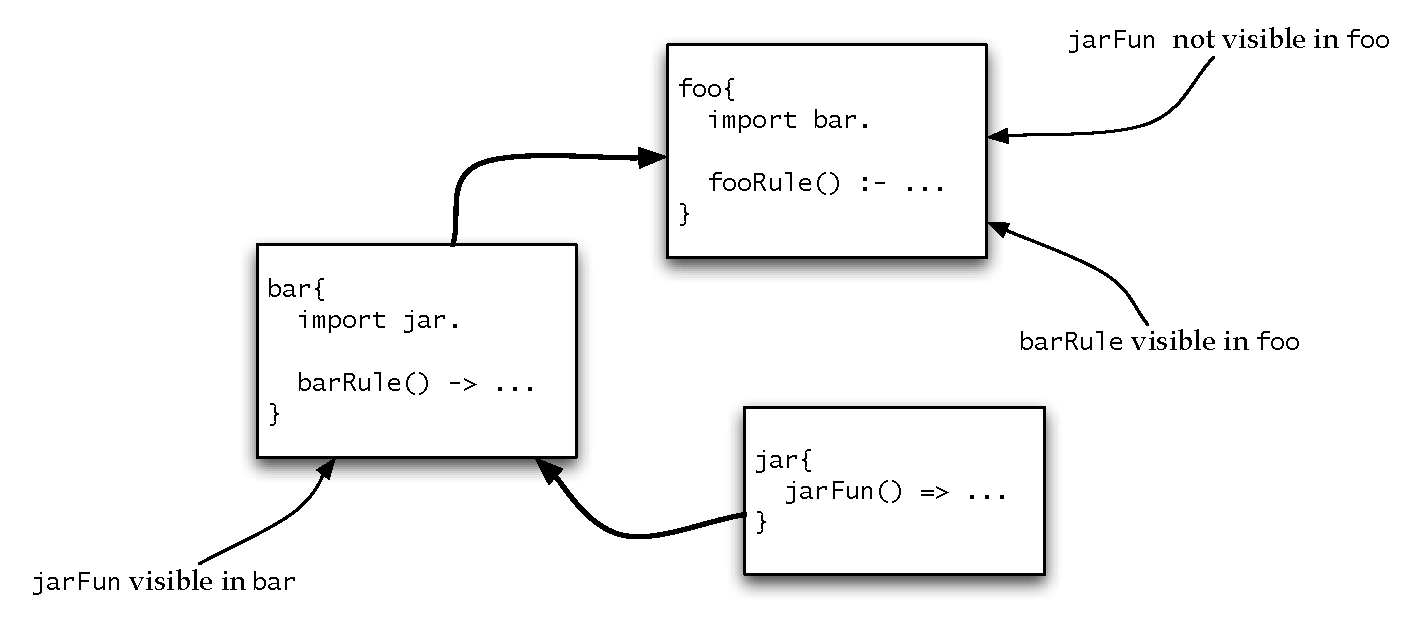
\includegraphics[width=\textwidth]{packages}
\end{boxed}
\caption{\label{program:packages:imports}A three-way package \q{import}}
\end{figure}
In this scenario \q{jarFun} is available within the \q{bar} package, but not in the \q{foo} package -- even though loading the \q{foo} package will cause \q{jar} to be loaded. If \q{jarFun} is required directly within the \q{foo} then it will have to be explicitly \q{import}ed by the \q{foo} package. Of course, the \q{barRule} action procedure is available within the \q{foo} package.

This can become an issue for type and other definitions that are shared over many packages. In that situation, the shared definitions will need to be \q{import}ed in each context that they are required.

\section{Top-level main programs}
\label{program:top-level}
Any package can also be treated as the top-level program -- provided that the package has a definition for the single argument action procedure \q{main}. In fact, \q{main} is a reserved word in \go: if a \q{main} program is defined in a package then it \emph{must} be consistent with the type assertion:
\begin{alltt}
main:[list[string]]*
\end{alltt}

If a package is executed at the top-level, then the \q{main} program in that package is executed and given as its single argument a list of the command-line arguments specified in the execution. For example, if a package \q{foo} were mentioned as the top-level package to execute in:
\begin{alltt}
\% go foo a b c
\end{alltt}
then the package \q{foo} must have an appropriate definition for \q{main} and that action procedure is entered -- with argument the list
\begin{alltt}["a","b","c"]\end{alltt}
\begin{aside}
Since the command line arguments are passed in as \q{string}s it is common for these argument strings to be parsed before they can be used in the application proper.  

The \q{\%\%} parse expression and the \q{go.stdparse} package become handy in this situation. For example, to pass a integer value to a \go fragment, where the number comes from the command line itself, then the classic way to do this is:
\begin{alltt}
mainPackage\{
  import go.stdparse.
  
  \ldots
  main([Arg,..More]) ->
    appProg(integerOf\%\%Arg);\ldots
\}
\end{alltt}
The \q{integerOf} grammar program parses a string into a \q{integer} value (see Section~\vref{stdparse:integerOf}).

See Chapter~\vref{compile} for further information on compiling and running \go programs.
\end{aside}

\section{Standard Packages}
\index{Packages!commonly loaded package}
Much of the functionality of the \go system is encapsulated in special packages that are not automatically included in every program. By convention, all \go system packages have package names of the form: \q{go.\emph{name}}; for example, the system input/output package is called \q{go.io}. To access the standard I/O package, then, it is necessary to load the \q{go.io} package:
\begin{alltt}
\emph{yourpackage}\{
  import go.io.
  
  \ldots
\}
\end{alltt}
\begin{aside}
The reason that \q{go.io} is not automatically included in every package is that that permits non-standard I/O systems to be used - for example in embedded applications, or in systems which have to interact with file systems in special ways.
\end{aside}
The standard set of packages will vary from time to time, the current set includes the packages
\begin{description}
\item[\q{go.cell}] Implements a re-assignable resource entity.
\item[\q{go.datelib}] Implements a collection of date related functions.
\item[\q{go.dynamic}] Implements dynamic relations; relations that can be updated.
\item[\q{go.hash}] Implements a hash-table package.
\item[\q{go.io}] Implements the standard I/O package
\item[\q{go.mbox}] Implements an internal thread communication package.
%\item[\q{go.scomms}] Implements a communication interface to the SCS.
\item[\q{go.setlib}] Implements a collection of set-like functions.
\item[\q{go.sort}] Implements a sort function
\item[\q{go.stack}] Implements a shareable updatable stack package.
\item[\q{go.queue}] Implements a shareable updatable queue package.
\item[\q{go.stdlib}] The standard \go language support package.\footnote{This package \emph{is automatically loaded} as it is required for successful execution of any \go program.}
\item[\q{go.stdparse}] Implements a range of parsing functions, allowing the conversion of strings to numbers, for example.
\item[\q{go.unit}] Implements a unit-testing framework.
\item[\q{go.xml}] Implements an XML parser and displayer package. Also defines the \go version of the DOM (Document Object Model).
\item[\q{go.http}] Implements many of the functions needed to build a Web server or an HTTP client.
\end{description}





%\chapter{Canonical \go}
\label{canonical}

\index{canonical form}
In a mirror image of the syntactic aspects of \go programs, the meaning of a \go program is broken down into several phases. In the first phase we map arbitrary \go programs into a much simpler \firstterm{canonical form}. Most of the \go language features -- such as equations, theta expressions and actions -- are eliminated from the canonical form of a program.\footnote{The \go compiler is even more aggressive in its mapping to a canonical form; in order to facilitate translation into simple machine instructions the compiler must ensure that the maximum `depth' of terms in a canonical program is no more that 1 -- i.e., it is not permissable to nest constructor terms. However, for the purposes of this discussion, such aggression is not required.} The second phase of giving a meaning to \go\ programs in canonical form.

Note that we present the canonicalization of \go programs for explanatory purposes only. Although based on \go, a canonical \go program is not typically a legal \go program; our purpose here is to define the \emph{operational meaning} of a \go program more precisely.

\section{Canonical \go programs}
\label{canonical:canonical}

Canonical \go programs have a much reduced form compared to normal \go programs: they are untyped, have no functions or functional expressions, no grammar rules, action rule or theta expressions. However, unlike in regular \go, \firstterm{types} may be represented explicitly in a canonical program.

The major program constructor in canonical \go is the clause:
\begin{alltt}
[V\sub1,\ldots,V\subn]-Term :- G\sub1,\ldots,G\sub{k}
\end{alltt}
We require an additional form of clause to adequately `capture' many of the committed choice forms of rules:
\begin{alltt}
[V\sub1,\ldots,V\subn]-Term::Cond :-- G\sub1,\ldots,G\sub{k}
\end{alltt}
which means that if the \q{Term} matches a goal \emph{G}, and \q{Cond} holds, then the goal \emph{G} is reduced to \emph{G\sub1,\ldots,G\subn}.

The fact that all \go programs can be mapped to such a simple form is part of our justification that \go's semantics may be grounded in a first order theory. However, we do leave one important logical feature `unexplained' in our transformation: recursive programs are represented in canonical \go as `circular terms'. This is for convenience only; it is certainly possible to eliminate these also.

Canonical \go clauses may be unioned together into a disjunction:
\begin{alltt}
\emph{Cl\sub1} | \ldots | \emph{Cl\subn}
\end{alltt}
and a \go \emph{canonical closure} is pair consisting of a union of canonical clauses and a list of pairs of variable names and terms -- these corresponding to the free variables and their values in the body of the union of clauses. We denote a canonical closure:
\begin{alltt}
< \emph{clause-union}, [ (fV\sub1,\emph{val\sub1}),\ldots,(fV\subn,\emph{val\subn})]>
\end{alltt}
where \q{'fv\subi'} are the free variables and \q{val\subi} are their corresponding values.

\index{free variables!in canonical form}
Note that, although the free variables' names are shown explicitly in the closure, in compiled code free variables are not identified in this way -- references to free variables become, as do references to local variables, offsets into a vector of the values of the free variables.

Calls in the body of a canonical clause take the form:
\begin{alltt}
\emph{Prog}(\emph{A\sub1},\ldots,\emph{A\subn})
\end{alltt}
where \emph{Prog} is either an identifier denoting a variable -- either local to the clause or a free variable in the innermost canonical closure -- or a literal union of clauses. In the latter case, the clauses in the literal union are assumed to share the same free variables as the canonical clause itself.

Canonical \go has a limited reportoire of data values: symbols, numbers, variables, lists, constructor terms and attribute sets. We will use normal \go notation to represent symbols, numbers, variables, lists and attribute sets; we use the normal function notation to represent a constructor term:
\begin{alltt}
\emph{F}(\emph{A\sub1},\ldots,\emph{A\subn})
\end{alltt}

One special type of term that is present in canonical \go clauses is the \emph{match pattern} which is written
\begin{alltt}
.\emph{Term}
\end{alltt}
The match pattern has the same `value' as the term that is embedded within it; except that semantically when unifying against a match pattern the `input term' is not permitted to be further instantiated. Any variables present in \emph{Term} may be bound, however.

In the following sections we show how all the major features of \go programs are mapped into canonical \go. Note that much of this chapter takes the form of \emph{definitions}; we are simply defining the meaning of \go programs in terms of canonical \go. This does not itself define \go's \emph{operational semantics} completely -- that requires giving a semantics to canonical \go itself; however, canonical \go is much simpler that `full \go'; and so it is easier to give an account of the declarative and operational semantics of canonical \go than `full \go'.

\section{Terms in canonical form}
\label{canonical:term}

\index{canonical form!of terms}

\subsection{Expressions}
\label{canonical:expressions}

\index{canonical form!expressions}
\index{expression!canonical form of}
The principal case in `expression handling' is the functional expression -- the application of a function to some arguments. 

Equations are mapped to canonical iff clauses with an additional argument; for example the function:
\begin{alltt}
app([],X) => X.
app([E,..X],Y) => [E,..app(X,Y)]
\end{alltt}
is mapped to the canonical clauses:
\begin{alltt}
( [X]-(.[],.X,X):--true
| [E,X,Y,\$1]-(.[E,..X],.Y,[E,..\$1]) :-- app(X,Y,\$1)
)
\end{alltt}
In general, a functional expression is mapped to a new variable and one or more new goals. The new variable represents the value computed by the function and the new goals represent calls to the canonicalized function itself.

The new goals must be inserted into the body of the canonical rule that arises from the canonicalization of the rule  containing the functional expression. The rules for the precise position of the new goal affects the `order of evaluation' rules of the functional expression itself:

\begin{itemize}
\item
If the functional expression occurs in a goal condition, then the new goal is placed before the canonicalized goal condition -- wherever it is eventually placed. It is placed \emph{after} any goal conditions that arise from canonicalizing the \emph{arguments} of the functional expression.

For example, a goal condition containing a functional  expression such as:
\begin{alltt}
\ldots,P(\ldots{}sort(app(A,B))\ldots),\ldots
\end{alltt}
is mapped to:
\begin{alltt}
\ldots,app(A,B,\$1),sort(\$1,\$2),\ldots,P(\ldots\$2\ldots),\ldots
\end{alltt}
The effect of this ordering rule is to impose a left-right depth-first evaluation of expressions; otherwise known as strict evaluation.

\item
If the functional expression occurs in an action or grammar rule body, then the rules are similar to those for goal conditions.

\item
If the functional expression occurs in the head of a clause, then the new goals are added to the end of the guard for that clause. (We shall see below, how guards are canonicalized).

For example, a clause such as:
\begin{alltt}
parent(X,parOf(X))
\end{alltt}
occurring within a theta environment is mapped to the clause:
\begin{alltt}
[X,\$1]-((X,\$1)::parOf(X,\$1):-true)
\end{alltt}
Functional expressions occurring within the heads of action rules and grammar rules are treated in a similar fashion.
\end{itemize}

\subsection{Patterns}
\label{canonical:pattern}

\index{canonical form!patterns}
\index{pattern!canonical form of}
Patterns occur in the heads of certain kinds of rules, in particular in the heads of equations, action rules, message receive clauses. In addition, the standard \go predicate \q{.=} has a pattern on the left hand side.

Patterns are different to terms in that it is not permitted to bind a variable `on the other side' of a pattern. In the case of patterns occurring in the heads of equations etc. this means that it is not permitted to bind a variable occurring in the function call (or procedure call or input message). In the case of the \q{.=} predicate, it is not permitted to bind variables occurring in the right hand side.

In addition, patterns have other restrictions -- evaluable expressions are not permitted in patterns. Patterns are restricted to variables, symbols, list patterns and constructor term patterns. On the other hand, \q{::} guarded patterns \emph{are} allowed. Furthermore, \go permits guard conditions in a guarded pattern to bind variables that would not otherwise be allowed.\footnote{This is, in part, due to the impossibility of checking against this.} 

\subsection{Attribute sets}
\label{canonical:attributes}

\index{canonical form!attribute sets}
\index{attribute sets!canonical form of}
On the whole the treatment of attribute sets is very similar to constructors: they are effectively left alone by canonicalization. 

A dot expression occurring in the head of a rule is treated as though it were a function call -- i.e., it is `broken out' into a separate goal. Other occurrences of dot expressions are left untouched.

\section{Goals}
\label{canonical:goals}

\section{Actions}
\label{canonical:actions}

\section{Grammars}
\label{canonical:grammars}

\section{Types}
\label{canonical:types}

\section{Theta environments}
\label{canonical:theta}


\part{Standard library}
The Standard library consists of the functions, predicates and actions that are part of the standard definition of \go. Note, however, that in order to access certain of these built-in functions it may be necessary to use explicit \function{import} directives.
\chapter{Arithmetic Primitives}

\go has two fundamental numeric types -- \q{integer} and \q{float}. These types are not in a sub-type relationship to each other; however, they are both sub types of the \q{number} type. I.e., the type lattice is defined by:
\begin{alltt}
integer\impl{}number.
float\impl{}number.
\end{alltt}
Most arithmetic functions are polymorphic where the arguments are a sub-type of \q{number}. For example, the \q{+} function is polymorphic, where both arguments must be either \q{integer} or \q{float} and returns a corresponding type.

Because there is no sub-type relationship between \q{float} and \q{integer} -- i.e., neither is a sub-type of the other -- it may be necessary to explicitly convert a value from one type to another. This conversion is not done automatically. The standard \q{n2float} function (see Section~\vref{arith:n2float}) can be used to convert from an \q{integer} to a \q{float} and the \q{itrunc} function (see Section~\vref{arith:itrunc}) converts -- with potential loss of precision -- from \q{float}ing point to \q{integer}.


Any exceptions raised by arithmetic primitives take the form:
\begin{alltt}
error(\emph{FunctionName},\emph{code})
\end{alltt}
where \q{\emph{code}} gives some indication of the kind of exception being raised. See Appendix~\vref{errorcodes} for a complete list of standard error codes.

\section{Basic arithmetic primitives}
\label{arith:basic}

\subsection{\function{+} -- Numeric addition}
\synopsis{+}{[T\impl{}number,T]\funarrow{}T}
\index{numeric addition}
\index{\q{+} operator}
\index{arithmetic!addition}
\index{operator!\q{+}}     
The \function{+} function expects two numeric arguments and returns their sum. 

The precise type associated with \q{+} bears further inspection: \q{+} is actually a polymorphic function -- defined over any kind of \q{number} value. However, the type of each argument should be the \emph{same} and the type of the result is also the same. Thus, \q{+} might be thought of as being several functions rolled into one: an integer-only addition and a floating point addition function.

\function{+} is a standard infix operator recognized by the \go\ compiler.
    
\paragraph{Error exceptions}\footnote{See Appendix~\vref{errorcodes} for the definition of the standard error codes}
\begin{description}
\item[\constant{'eINSUFARG'}]
At least one of the arguments is uninstantiated.
\end{description}

\subsection{\function{-} -- Numeric subtraction}
\synopsis{-}{[T\impl{}number,T]\funarrow{}T}
The \function{-} function expects two numeric arguments and returns the result of subtracting \param{Y} from \param{X}.

Note that unary arithmetic negation is equivalent to subtracting the negated expression from 0 (or 0.0 depending on the type of the negated expression).

Like \q{+}, \q{-} is actually a polymorphic function, separately handling \q{integer} and \q{float}ing point arithmetic.
    
\function{-} is a standard operator recognized by the \go\ compiler.
    
\paragraph{Error exceptions}
\begin{description}
\item[\constant{'eINSUFARG'}]
At least one of the arguments is uninstantiated.
\end{description}

\subsection{\function{*} -- Numeric product}
\synopsis{*}{[T\impl{}number,T]\funarrow{}T}
The \function{*} function expects two numeric arguments and returns their product.
    
Like \q{+}, \q{*} is actually a polymorphic function, separately handling \q{integer} and \q{float}ing point arithmetic.

\function{*} is a standard operator recognized by the \go\ compiler.
    
\paragraph{Error exceptions}
\begin{description}
\item[\constant{'eINSUFARG'}]
At least one of the arguments is uninstantiated.
\end{description}

\subsection{\function{/} -- Numeric division}
\synopsis{/}{[T\impl{}number,T]\funarrow{}T}
The \function{/} function expects two numeric arguments and returns the result of dividing \param{X} by \param{Y}.
    
Like other arithmetic functions, \q{/} is actually a polymorphic function, separately handling \q{integer} and \q{float}ing point arithmetic.

\function{/} is a standard operator recognized by the \go\ compiler.
    
\paragraph{Error exceptions}
\begin{description}
\item[\constant{'eINSUFARG'}]
At least one of the arguments is uninstantiated.
\item[\constant{'eIDIVZERO'}]
\param{Y} is zero, or too close to zero
\end{description}

\subsection{\function{quot} -- Integer quotient}
\synopsis{quot}{[T\impl{}number,T]\funarrow{}integer}
The \function{quot} function expects two numeric arguments and returns the integer quotient of dividing \param{X} by \param{Y}.
    
Like other arithmetic functions, \q{quot} is a polymorphic function, separately handling \q{integer} and \q{float}ing point arithmetic. However, it always returns an \q{integer} result.

\function{quot} is a standard operator recognized by the \go\ compiler.
    
\paragraph{Error exceptions}
\begin{description}
\item[\constant{'eINSUFARG'}]
At least one of the arguments is uninstantiated.
\item[\constant{'eIDIVZERO'}]
\param{Y} is zero, or too close to zero
\end{description}

\subsection{\function{rem} -- Remainder}
\synopsis{rem}{[T\impl{}number,T]\funarrow{}float}
The \function{rem} function expects two numeric arguments and returns the remainder of the integer quotient of dividing \param{X} by \param{Y}. Note that while \function{quot} will always return an integral value, \function{rem} will always return a \q{float}.
    
\function{rem} is a standard operator recognized by the \go\ compiler.
    
\paragraph{Error exceptions}
\begin{description}
\item[\constant{'eINSUFARG'}]
At least one of the arguments is uninstantiated.
\item[\constant{'eIDIVZERO'}]
\param{Y} is zero, or too close to zero
\end{description}

\subsection{\function{abs} -- Absolute value}
\synopsis{abs}{[T\impl{}number]\funarrow{}T}
The \function{abs} function expects a numeric argument and returns the absolute value of \param{X}. The type of the returned value is the same as the argument: the absolute value of an \q{integer} is an \q{integer} and likewise for a \q{float}.
     
\paragraph{Error exceptions}
\begin{description}
\item[\constant{'eINSUFARG'}]
At least one of the arguments is uninstantiated.
\end{description}

\subsection{\function{**} -- Exponentiation}
\synopsis{**}{[T\impl{}number,T]\funarrow{}T}
The \function{**} function expects two numeric arguments and returns the result of raising \param{X} to the power \param{Y}; i.e., $\param{X}^\param{Y}$.
    
\function{**} is a standard operator recognized by the \go\ compiler.
    
\paragraph{Error exceptions}
\begin{description}
\item[\constant{'eINSUFARG'}]
At least one of the arguments is uninstantiated.
\item[\constant{'eINVAL'}]
\param{Y} is negative, and \param{X} is zero, or too close to zero
\end{description}

\subsection{\function{integral} -- Integer predicate}
\synopsis{integral}{[T\impl{}number]\{\}}
The \function{integral} predicate succeeds if its parameter is an integer; fails if it is a fractional value, or an integer that cannot be represented as a integer. This last point is important for large values; a number such as $1\times10^{200}$ is integral from a mathematical point of view, but it cannot be represented as a 64 bit integer and so would \emph{fail} the \function{integral} test.

This predicate will accept either \q{integer} or \q{float} values. However, it is clearly trivial for \q{integer} arguments.
    
\paragraph{Error exceptions}
\begin{description}
\item[\constant{'eINSUFARG'}]
The argument must be a number, variables are not permitted.
\end{description}

\subsection{\function{trunc} -- Extract integral part}
\synopsis{trunc}{[T\impl{}number]\funarrow{}T}
The \function{trunc} returns the nearest integer value to its input. It works for all number values (including very large numbers) representable by \go. Note that not all integral values are representable as \q{integer}s -- especially very large values, with an absolute value larger than $2^{63}$. Such large values must still be represented as \q{float}ing point numbers.

\paragraph{Error exceptions}
\begin{description}
\item[\constant{'eINSUFARG'}]
The argument must be a number, variables are not permitted.
\end{description}

\subsection{\function{itrunc} -- Extract integral part}
\label{arith:itrunc}
\synopsis{itrunc}{[T\impl{}number]\funarrow{}integer}
The \function{trunc} returns the nearest integer value to its input. The value returned is an \q{integer}.

\paragraph{Error exceptions}
\begin{description}
\item[\constant{'eINSUFARG'}]
The argument must be a number, variables are not permitted.
\end{description}

\subsection{\function{floor} -- Largest integer that is smaller}
\synopsis{floor}{[T\impl{}number]\funarrow{}T}
The \function{floor} returns the nearest integer value that is the same or smaller than its input.

\paragraph{Error exceptions}
\begin{description}
\item[\constant{'eINSUFARG'}]
The argument must be a number, variables are not permitted.
\end{description}

\subsection{\function{ceil} -- Smallest integer that is larger}
\synopsis{ceil}{[T\impl{}number]\funarrow{}T}
The \function{ceil} returns the smallest integer value that is the same or larger than its input.

\paragraph{Error exceptions}
\begin{description}
\item[\constant{'eINSUFARG'}]
The argument must be a number, variables are not permitted.
\end{description}

\subsection{\function{n2float} -- Convert to float}
\label{arith:n2float}
\synopsis{n2float}{[T\impl{}number]\funarrow{}float}
The \function{n2float} `converts' a number (either an \q{integer} or a \q{float}) into a \q{float}ing point equivalent.

\paragraph{Error exceptions}
\begin{description}
\item[\constant{'eINSUFARG'}]
The argument must be a number, variables are not permitted.
\end{description}


\section{Modulo arithmetic}
\label{arith:modulo}

The modulo arithmetic primitives perform their arithmetic in a modulo range. This means that their arguments must be integer and the results are always constrained to be integers in the range $0..M-1$ where $M$ is the modulus. If the modulus argument is 0 then the arithmetic is assumed to be at the precision of the machine (typically 64 bits)

\subsection{\function{iplus} -- modulo addition}
\synopsis{iplus}{[integer,integer,integer]\funarrow{}integer}
The \function{iplus} function expects three \q{integer} arguments and returns the sum of the first two modulo the third; i.e., \q{iplus(X,Y,M)} evaluates to $(X+Y)|_M$.
        
\paragraph{Error exceptions}
\begin{description}
\item[\constant{'eINSUFARG'}]
At least one of the arguments is uninstantiated.
\item[\constant{'eINTNEEDD'}]
At least one of the arguments is not an integer.
\end{description}

\subsection{\function{iminus} -- modulo subtraction}
\synopsis{iminus}{[integer,integer,integer]\funarrow{}integer}
The \function{iminus} function expects three \q{integer} arguments and returns the result of subtracting the second from the first, modulo the third; i.e., the value of \q{iminus(X,Y,M)} is $(X-Y)|_M$.
        
\paragraph{Error exceptions}
\begin{description}
\item[\constant{'eINSUFARG'}]
At least one of the arguments is uninstantiated.
\item[\constant{'eINTNEEDD'}]
At least one of the arguments is not an integer.
\end{description}

\subsection{\function{itimes} -- modulo multiplication}
\synopsis{itimes}{[integer,integer,integer]\funarrow{}integer}
The \function{itimes} function expects three \q{integer} arguments and returns the result of multiplying the first two arguments, modulo the third; i.e., the value of \q{itimes(X,Y,M)} is $(X*Y)|_M$.
        
\paragraph{Error exceptions}
\begin{description}
\item[\constant{'eINSUFARG'}]
At least one of the arguments is uninstantiated.
\item[\constant{'eINTNEEDD'}]
At least one of the arguments is not an integer.
\end{description}

\subsection{\function{idiv} -- modulo division}
\synopsis{idiv}{[integer,integer,integer]\funarrow{}integer}
The \function{idiv} function expects three \q{integer} arguments and returns the result of dividing the first two arguments, modulo the third; i.e., the value of \q{idiv(X,Y,M)} is $(X/Y)|_M$.
The integer quotient of the division is returned.
        
\paragraph{Error exceptions}
\begin{description}
\item[\constant{'eINSUFARG'}]
At least one of the arguments is uninstantiated.
\item[\constant{'eINTNEEDD'}]
At least one of the arguments is not an integer.
\end{description}

\subsection{\function{imod} -- modulus }
\synopsis{imod}{[integer,integer]\funarrow{}integer}
The \function{imod} function expects two \q{integer} arguments and returns modulo result of the frist argument; i.e., \q{imod(X,M)} evaluates to $X|_M$.
        
\paragraph{Error exceptions}
\begin{description}
\item[\constant{'eINSUFARG'}]
At least one of the arguments is uninstantiated.
\item[\constant{'eINTNEEDD'}]
At least one of the arguments is not an integer.
\end{description}

\section{Bit Oriented Arithmetic Primitives}
All the bit oriented functions take \q{integer} arguments, and return \q{integer} results.

\subsection{\function{band} -- Bitwise and function}
\label{arith:band}
\synopsis{band}{[integer,integer]\funarrow{}integer}
The \function{band} function expects two integer arguments and returns their binary bitwise intersection.
        
\paragraph{Error exceptions}
\begin{description}
\item[\constant{'eINSUFARG'}]
At least one of the arguments is uninstantiated.
\item[\constant{'eINTNEEDD'}]
At least one of the arguments is not an integer -- i.e., is not representable as a 64 bit integer.
\end{description}

\subsection{\function{bor} -- Bitwise or function}
\synopsis{bor}{[integer,integer]\funarrow{}integer}
The \function{bor} function takes two integer arguments and returns their binary bitwise union.
        
\paragraph{Error exceptions}
\begin{description}
\item[\constant{'eINSUFARG'}]
At least one of the arguments is uninstantiated.
\item[\constant{'eINTNEEDD'}]
At least one of the arguments is not an integer -- i.e., is not representable as a 64 bit integer.
\end{description}

\subsection{\function{bnot} -- Binary negation}
\synopsis{bnot}{[integer]\funarrow{}integer}
The \function{bnot} function expects an integer argument and returns its binary bitwise 1's complement.
        
\paragraph{Error exceptions}
\begin{description}
\item[\constant{'eINSUFARG'}]
The argument is uninstantiated.
\item[\constant{'eINTNEEDD'}]
The argument is not an integer -- i.e., is not representable as a 64 bit integer.
\end{description}
      
\subsection{\function{bxor} -- Bitwise exclusive or function}
\synopsis{bxor}{[integer,integer]\funarrow{}integer}
The \function{band} function expects two integer arguments and returns their binary bitwise exclusive or.
        
\paragraph{Error exceptions}
\begin{description}
\item[\constant{'eINSUFARG'}]
At least one of the arguments is uninstantiated.
\item[\constant{'eINTNEEDD'}]
At least one of the arguments is not an integer -- i.e., is not representable as a 64 bit integer.
\end{description}
      
\subsection{\function{bleft} -- Bitwise left shift function}
\synopsis{bleft}{[integer,integer]\funarrow{}integer}
The \function{bleft} function expects two integer arguments and returns result of leftshifting the first argument; i.e., \q{bleft(X,Y)} evaluates to $X*2^{Y}$. The number is right-filled with zero.

\paragraph{Error exceptions}
\begin{description}
\item[\constant{'eINSUFARG'}]
At least one of the arguments is uninstantiated.
\item[\constant{'eINTNEEDD'}]
At least one of the arguments is not an integer -- i.e., is not representable as a 64 bit integer.
\end{description}
      
\subsection{\function{bright} -- Bitwise right shift function}
\synopsis{bright}{[integer,integer]\funarrow{}integer}
The \function{bright} function expects two integer arguments and returns result of rightshifting the first argument by the second; i.e., \q{bright(X,Y)} evaluates to $X/2^{Y}$. The result is sign-extended -- if the original number is negative then the result is also negative.

\paragraph{Error exceptions}
\begin{description}
\item[\constant{'eINSUFARG'}]
At least one of the arguments is uninstantiated.
\item[\constant{'eINTNEEDD'}]
At least one of the arguments is not an integer -- i.e., is not representable as a 64 bit integer.
\end{description}

\section{Arithmetic inequalities}
\label{arith:ineq}

Basic inequality predicates such as \function{<}.
  
\subsection{\function{<} -- Less than predicate}
\synopsis{<}{[T\impl{}number,T]\{\}}
The \function{<} predicate expects two arguments and succeeds if the first is smaller than the second. Like many of the arithmetic functions, the arithmetic predicates are polymorphic, but require both arguments to be of the same type. 

\q{<} is a standard operator, and \q{<} predicates are written in infix notation.
    
\paragraph{Error exceptions}
\begin{description}
\item[\constant{'eINVAL'}]
An attempt to compare incomparible values -- such as variables.
\end{description}

\subsection{\function{=<} -- Less than or equal predicate}
\synopsis{=<}{[T\impl{}number,T]\{\}}
The \function{=<} predicate expects two arguments and succeeds if the first argument is smaller than or equal to the second.
    
\q{=<} is a standard operator, and \q{=<} predicates are written in infix notation.

\paragraph{Error exceptions}
\begin{description}
\item[\constant{'eINSUFARG'}]
At least one of the arguments is uninstantiated.
\end{description}

\subsection{\function{>} -- Greater than predicate}
\synopsis{>}{[T\impl{}number,T]\{\}}
The \function{>} predicate expects two arguments and succeeds if the first argument is greater than the second.
    
\q{>} is a standard operator, and \q{>} predicates are written in infix notation.

\paragraph{Error exceptions}
\begin{description}
\item[\constant{'eINSUFARG'}]
At least one of the arguments is uninstantiated.
\end{description}

\subsection{\function{>=} -- Greater than or equal predicate}
\synopsis{>=}{[T\impl{}number,T]\{\}}
The \function{>=} predicate expects two numeric arguments and succeeds if the first argument is greater, or equal to, the second.
    
\q{>=} is a standard operator, and \q{>=} predicates are written in infix notation.

\paragraph{Error exceptions}
\begin{description}
\item[\constant{'eINSUFARG'}]
At least one of the arguments is uninstantiated.
\end{description}

\section{Trigonometric functions}
\label{arith:trig}
The trigonometric functions generally accept either \q{integer} or \q{float} arguments. However, they will always \emph{return} a \q{float} result.

\subsection{\function{sin} -- Sine function}
\label{arith:sin}
\synopsis{sin}{[number]\funarrow{}float}
The \function{sin} function returns the sin of its argument -- interpreted in radians. The value of \q{sin} is only reliable if its argument in the range $[-2\pi,2\pi]$.
        
\paragraph{Error exceptions}
\begin{description}
\item[\constant{'eINSUFARG'}]
The argument is uninstantiated.
\end{description}

\subsection{\function{asin} -- Arc Sine function}
\label{arith:asin}
\synopsis{asin}{[number]\funarrow{}float}
The \function{asin} function returns the arc sin of its argument. The returned value will be in the range $[-\pi/2,\pi/2]$.
        
\paragraph{Error exceptions}
\begin{description}
\item[\constant{'eINSUFARG'}]
The argument is uninstantiated.
\item[\constant{'eRANGE'}]
The parameter is out of range.
\item[\constant{'eINVAL'}]
\end{description}

\subsection{\function{cos} -- Cosine function}
\label{arith:cos}
\synopsis{cos}{[number]\funarrow{}float}
     
The \function{cos} function returns the cosine of its argument -- interpreted in radians. \q{cos(X)} is only reliable if \q{X} is in the range $[0,\pi]$.
        
\paragraph{Error exceptions}
\begin{description}
\item[\constant{'eINSUFARG'}]
The argument is uninstantiated.
\end{description}

\subsection{\function{acos} -- Arc Cosine function}
\label{arith:acos}
\synopsis{acos}{[number]\funarrow{}float}
The \function{acos} function returns the arc cosine of its argument in radians. 
        
\paragraph{Error exceptions}
\begin{description}
\item[\constant{'eINSUFARG'}]
The argument is uninstantiated.
\item[\constant{'eRANGE'}]
The parameter is out of range.
\item[\constant{'eINVAL'}]
\end{description}

\subsection{\function{tan} -- Tangent function}
\label{arith:tan}
\synopsis{tan}{[number]\funarrow{}float}
The \function{tan} function returns the tangent of its argument -- interpreted in radians.  \q{atan} requires its argument to be in the range $[-\pi/2,\pi/2]$.
        
        
\paragraph{Error exceptions}
\begin{description}
\item[\constant{'eINSUFARG'}]
The argument is uninstantiated.
\end{description}

\subsection{\function{atan} -- Arc Tangent function}
\label{arith:atan}
\synopsis{atan}{[number]\funarrow{}float}
     
The \function{atan} function returns the arc tangent of its argument.
\paragraph{Error exceptions}
\begin{description}
\item[\constant{'eINSUFARG'}]
The argument is uninstantiated.
\item[\constant{'eRANGE'}]
The parameter is out of range.
\item[\constant{'eINVAL'}]
\end{description}

\subsection{\function{pi} -- return \texorpdfstring{$\pi$}{pi}}
\label{arith:pi}

\synopsis{pi}{()\funarrow{}float}
The \q{pi} function returns $\pi$, accurate to the resolution of the underlying IEEE floating point arithmetic.

\section{Other math functions}
\label{arith:other}


\subsection{\function{irand} -- random integer generator}
\label{arith:irand}

\synopsis{irand}{[integer]\funarrow{}integer}
The \function{irand} function returns a random \q{integer} in the range $[0\ldots\param{X}-1]$, where $X$ is its argument. The value of \param{X} should be non-negative.
        
\paragraph{Error exceptions}
\begin{description}
\item[\constant{'eINSUFARG'}]
The argument is uninstantiated.
\item[\constant{'eINVAL'}]
A negative number is not permitted for \q{irand}
\end{description}

\subsection{\function{rand} -- random number generator}
\label{arith:rand}

\synopsis{rand}{[number]\funarrow{}float}
The \function{rand} function returns a random \q{float}ing point number in the range $[0\ldots\param{X})$, where \param{X} is its argument -- which may be either \q{integer} or \q{float}. The value of \param{X} should be non-negative.
        
\paragraph{Error exceptions}
\begin{description}
\item[\constant{'eINSUFARG'}]
The argument is uninstantiated.
\item[\constant{'eINVAL'}]
A negative number is not permitted for \q{rand}
\end{description}

\subsection{\function{srand} -- seed random number generation}
\label{arith:srand}

\synopsis{srand}{[number]*}
     
The \function{srand} action `seeds' the random number generator with its \q{number} argumnent, which should be non-negative. \q{srand} can be used to either ensure a repeatable sequence (by seeding it with a fixed known value) or to ensure a more random, non-repeatable, sequence by seeding it with a value that is always different -- such as the current time.
        
\paragraph{Error exceptions}
\begin{description}
\item[\constant{'eINSUFARG'}]
The argument is uninstantiated.
\item[\constant{'eINVAL'}]
A negative number is not permitted for \q{srand}
\end{description}

\subsection{\function{sqrt} -- square root function}
\label{arith:sqrt}

\synopsis{sqrt}{[number]\funarrow{}float}
     
The \function{sqrt} function returns the square root of its argument -- which should be non-negative. The argument may be either an \q{integer} or a \q{float}; however, the result is always a \q{float}.
        
\paragraph{Error exceptions}
\begin{description}
\item[\constant{'eINSUFARG'}]
The argument is uninstantiated.
\item[\constant{'eINVAL'}]
A negative number is not permitted for \q{sqrt}
\end{description}

\subsection{\function{exp} -- exponentiation function}
\label{arith:exp}

\synopsis{exp}{[number]\funarrow{}float}
     
The \function{exp} function returns $e^{\param{X}}$, where \param{X} is its non-negative argument.
        
\paragraph{Error exceptions}
\begin{description}
\item[\constant{'eINSUFARG'}]
The argument is uninstantiated.
\item[\constant{'eRANGE'}]
The parameter is out of range; it causes an overflow to exponentiate it.
\end{description}

\subsection{\function{log} -- natural logarithm function}
\label{arith:log}

\synopsis{log}{[number]\funarrow{}float}
     
The \function{log} function returns $\log_e({\param{X})}$. Its argument should be non-negative.
        
\paragraph{Error exceptions}
\begin{description}
\item[\constant{'eINSUFARG'}]
The argument is uninstantiated.
\item[\constant{'eRANGE'}]
The parameter is out of range.
\end{description}

\subsection{\function{log10} -- decimal logarithm function}
\label{arith:log10}

\synopsis{log10}{[number]\funarrow{}float}
     
The \function{log} function returns $\log_{10}({\param{X})}$.  Its argument should be non-negative.
        
\paragraph{Error exceptions}
\begin{description}
\item[\constant{'eINSUFARG'}]
The argument is uninstantiated.
\item[\constant{'eRANGE'}]
The parameter is out of range.
\end{description}

\section{Floating point manipulation}
\label{arith:manip}

These functions give special manipulation of floating point numbers; they are commonly used in converting between floating point numbers and strings: either for parsing a string into a numeric value or in ddisplaying a number as a string.

\subsection{\function{ldexp} -- multiply by power of 2}
\label{arith:ldexp}

\synopsis{ldexp}{[float,float]\funarrow{}float}

The expression \q{ldexp(X,Y)} evaluates to $X\times2^{Y}$. This is useful in converting between string representations of numbers and floating point numbers themselves.

\paragraph{Error exceptions}
\begin{description}
\item[\constant{'eINSUFARG'}]
The argument is uninstantiated.
\end{description}

\subsection{\function{frexp} -- split into fraction and mantissae}
\label{arith:frexp}

\synopsis{frexp}{[float+,float-,integer-]\{\}}

This predicate is satisfied if the fractional part of the first parameter -- \param{X} -- is equal to the second parameter -- \param{F} -- with the third parameter -- \param{E} -- equal to its exponent. More specifically, \param{F} should be a \emph{normalized} number -- i.e., its absolute value is in the range $[0.5,1)$, or zero -- and \q{frexp(X,F,E)} is satisfied if
\[
X=F\times2^{E} \wedge ( F=0 \vee |F| \epsilon [0.5,1) )
\]
If \param{X} is zero, then both \param{F} and \param{E} should also be zero.

Although a predicate, the modes in this type definition indicate that \param{X} must be given and both \param{F} and \param{E} are output.

\paragraph{Error exceptions}
\begin{description}
\item[\constant{'eINSUFARG'}]
The argument \param{X} is uninstantiated.
\end{description}

\subsection{\function{modf} -- split into integer and fraction parts}
\label{arith:modf}

\synopsis{modf}{[flaot+,float-,float-]\{\}}

A predication \q{modf(X,I,F)} is satisfied if the integer part of \param{X} is \param{I} and the fractional part is \param{F}. More specifically,  $X=I+F$, and \param{I} is integral.

Although a predicate, the modes indicate that \param{X} must be given and both \param{I} and \param{F} are output.

This primitive is particularly useful when displaying floating point numbers.

\paragraph{Error exceptions}
\begin{description}
\item[\constant{'eINSUFARG'}]
The argument \param{X} is uninstantiated.
\end{description}


\chapter{Standard Library}
\label{stdlib}
The standard libraries contain suites of programs that are useful in many different situations. 

For many of the functions in this library, it is not necessary to explicitly \q{import} the corresponding packages. In fact, these programs are defined in the standard library \q{go.stdlib} -- which is always automatically loaded for all programs.

However, some functions are in separate packages and will need to be explicitly \q{import}ed. All the packages in the standard library are part of the \q{go} package domain, and thus require an \q{import} statement of the form:
\begin{alltt}
\emph{packageName}\{
  import go.\emph{library}.
  \ldots
\}
\end{alltt}
Where a function requires a specific package to be \q{import}ed, the description of the function explains which package to load.

\section{List manipulation}
\go has a simple set of functions that can be used to manipulate lists. These are essentially culled from experience of what list functions are most used; of these list append (\q{<>}) is probably the most heavily used list function.

\subsection{\function{<>} -- List append}
\label{stdlib:append}
\synopsis{<>}{[list[t],list[t]]\funarrow{}list[t]}
\index{<>@\q{<>} function}
\index{Appending lists!with \q{<>} function}

The \q{<>} polymorphic function appends its two arguments together: both arguments being lists of the same type. The definition of list append is quite short:
\begin{alltt}
[] <> X => X.
[E,..X] <> Y => [E,..X<>Y].
\end{alltt}
As with many of the programs in the standard library, the \emph{name} of the function is also an operator; allowing the use of infix notation in list append expressions.

\subsection{\q{append} -- List append predicate}
\label{stdlib:app}
\synopsis{append}{[list[t],list[t],list[t]]\{\}}
\index{append@\q{append} predicate}
\index{Appending lists!with \q{append} predicate}

The \q{<>} list append function is convenient to use for the large majority of cases where it is used to concatenate two lists together. However, the traditional \prolog \q{append} predicate can be used for many additional things -- such as splitting lists, searching lists and so on. It is defined as:
\begin{alltt}
append([],X,X).
append([E,..X],Y,[E,..Z]):-append(X,Y,Z).
\end{alltt}

\subsection{\function{listlen} -- Length of a list}
\label{stdlib:listlen}
\index{length of a list}
\index{{\tt listlen} function}
\synopsis{listlen}{[list[t]]\funarrow{}integer)}

The \q{listlen} function counts the length of the list \param{L}. \q{listlen} is defined as though by:
\begin{alltt}
listlen(L) => len(L,0).

private len:[list[t],integer]=>integer.
len([],C) => C.
len([\_,..L],C) => len(L,C+1).
\end{alltt}

\subsection{\function{in} -- List membership}
\label{stdlib:in}
\synopsis{in}{[T,list[T]]\{\}}
\index{in@\q{in} predicate}
\index{Test for list membership}

The \q{in} standard predicate is true if the left hand argument term is on the list in the right hand argument.

The definition of \q{in} is:
\begin{alltt}
X in [X,..\_].
X in [\_,..Y] :- X in Y.
\end{alltt}
Note that unification is used to determine element equality, and that an element may be on a list more than once: the \q{in} predicate will find subsequent entries on backtracking.
\begin{aside}
If you look for the definition of \q{in} in the \q{go.stdlib} package source you will not find it. This is because \q{in} has such a deep relationship to many of \go's features that the compiler generates specific versions of \q{in} whenever it is used.
\end{aside}

\subsection{\function{reverse} -- List reverse}
\label{stdlib:rev}
\synopsis{reverse}{[list[t]]\funarrow{}list[t]}
\index{reverse@\q{reverse} a list function}
\index{Function to reverse lists}

The \q{reverse} polymorphic function reverses its argument. This is \emph{not} `naive reverse'; \q{rev} is a linear complexity function. The definition of \q{rev} uses an auxilliary function to accomplish list reversal:
\begin{alltt}
reverse(L) => rv(L,[]).

private rv:[list[t],list[t]]=>list[t].
rv([],R) => R.
rv([E,..M],R) => rv(M,[E,..R]).
\end{alltt}

\subsection{\function{nth} -- Nth element of a list}
\label{misc:nth}
\index{Nth element of a list}
\index{nth@\q{nth} function}

\synopsis{nth}{[list[T],integer]\funarrow{}t}

The \q{nth} function returns the n$^{th}$ element of a list. The definition of \q{nth} is:
\begin{alltt}
nth(L,\_)::var(L)=>exception error("nth",'eINVAL').
nth([E,..\_],1) => E.
nth([\_,..L],N) => nth(L,N-1).
nth([],\_) => raise error("nth",'eNOTFND').
\end{alltt}

\subsection{\q{front} -- the front portion of a list}
\label{stdlib:front}
\index{front@\q{front} of list function}
\index{Get front portion of list}
\synopsis{front}{[list[t],integer]\funarrow{}list[t]}

The \q{front} function returns the front portion of a list. It is defined as though by:
\begin{alltt}
front([],\_)=>[].
front([E,..L],C)::C>0 => [E,..front(L,C-1)].
front(\_,\_) => [].
\end{alltt}

\subsection{\q{tail} -- the tail portion of a list}
\label{stdlib:tail}
\index{tail@\q{tail} of list function}
\index{Get back portion of list}
\synopsis{tail}{[list[t],integer]\funarrow{}list[t]}

The \q{tail} function returns the tail portion of a list, i.e., the last N elements of the list. It is defined as though by:
\begin{alltt}
tail(L,C)::append(_,Tl,L), listlen(Tl,C) => Tl.
\end{alltt}
Note that its actual definition is significantly more efficient than this specification!

\subsection{\q{drop} -- drop n elements from a list}
\label{stdlib:drop}
\index{drop@\q{drop} from list function}
\synopsis{drop}{[list[t],integer]\funarrow{}list[t]}

The \q{drop} function drops the first N elements from a list. It is defined as:
\begin{alltt}
drop:[list[t],integer]=>list[t].

drop([],_)=>[].
drop(L,0) => L.
drop([_,..L],N) => drop(L,N-1).
\end{alltt}


\subsection{\function{iota} -- List construction}
\label{stdlib:iota}
\index{{\tt iota} function}
\index{construct a list of integers}

\synopsis{iota}{[integer,integer]\funarrow{}list[integer]}

The \q{iota} function constructs a list of integers from \param{X} to \param{Y} inclusive. The definition of \q{iota} is:
\begin{alltt}
iota(N,M)::N>M=>[].
iota(N,M)=>[N,..iota(N+1,M)].
\end{alltt}

\section{Set manipulation}
These programs support sets, represented as lists. Sets are not a fully first-class structure in \go: there is no built in set data type. However, it is perhaps more useful to provide a suite of functions that implement set-like semantics over lists. In addition to these functions, \go also has two specific operators for constructing set-like lists: the bag-of expression (see section~\vref{expression:bagof}) and the bounded set expression (see section~\vref{expression:bounded}).

These set functions are accessed via the \q{setlib} library:

\libsynopsis{go.setlib}

\subsection{\texorpdfstring{\function{\union} -- }{}Set union}
\label{stdlib:union}
\synopsis{\union}{[list[t],list[t]]\funarrow{}list[t]}

The \q{\union} (pronounced `union') function unions two sets -- represented as lists -- together. Note that the \union function assumes that both arguments are already sets -- i.e., do not contain duplicate elements.

The definition of \q{\union} is:
\begin{alltt}
[]\union{}X=>X.
[E,..X]\union{}Y :: E in Y => X\union{}Y.
[E,..X]\union{}Y => [E,..X\union{}Y].
\end{alltt}

\subsection{\texorpdfstring{\function{\intersection} -- }{}Set intersection}
\label{stdlib:intersection}
\synopsis{\intersection}{[list[t],list[t]]\funarrow{}list[t]}

The \q{\intersection} (pronounced `intersection') function intersects two sets -- represented as lists -- together. Note that the \intersection function assumes that both arguments are already sets -- i.e., do not contain duplicate elements.

The definition of \q{\intersection} is:
\begin{alltt}
[]\intersection{}\_=>[].
[E,..X]\intersection{}Y :: E in Y=> [E,..X\intersection{}Y].
[E,..X]\intersection{}Y => X\intersection{}Y.
\end{alltt}

\subsection{\texorpdfstring{\function{\difference} -- }{}Set difference}
\label{stdlib:difference}
\synopsis{\difference}{[list[t],list[t]]\funarrow{}list[t]}

The \q{\difference} (pronounced `difference') function forms the set difference of two sets -- represented as lists -- together. Note that the \difference function assumes that both arguments are already sets -- i.e., do not contain duplicate elements.

The definition of \q{\difference} is:
\begin{alltt}
[]\difference{}\_=>[].
[E,..X]\difference{}Y :: \nasf{}E in Y => [E,..X\difference{}Y].
[E,..X]\difference{}Y => X\difference{}Y.
\end{alltt}

\subsection{\texorpdfstring{\function{subset} -- }{}Subset predicate}
\label{setlib:subset}
\synopsis{subset}{[list[t],list[t]]\{\}}

The \q{subset} predicate is true if every element of the first list is also an element of the second.

For example:
\begin{alltt}
subset([1,34],[1,2,34,10,34,21,-3])
\end{alltt}
is satisfied, whereas
\begin{alltt}
subset([1,3,35],[1,2,34,10,34,21,-3])
\end{alltt}
is not, as \q{35} is not an element of the second argument.

The definition of \q{subset} is:
\begin{alltt}
subset(X,Y) :-
  E in X *> E in Y
\end{alltt}


\chapter{Character Primitives}
\label{chars}

\index{character primitives}
This chapter provides a reference for the standard character primitives of the \go\ language. The standard predicates define a number character classes as well as other attributes on characters.

The standard type for a character is \q{char}, and strings are of type \q{char[]}. \go's characters are based on the Unicode standard.

\section{Basic character class primitives}
\label{chars:charclass}

\subsection{\function{\_\_isCcChar} -- Other, control character}
\synopsis{\_\_isCcChar}{[char+]\{\}}
\label{chars:isCcChar}

\index{\q{\_\_isCcChar} predicate}
\index{character!Other control category}
\index{UNICODE!Other control category}
The \function{\_\_isCcChar} predicate tests to see if its \type{char} argument represents a character in the Unicode `Other, Control' general category. This includes the normal ASCII control characters.
        
\paragraph{Error exceptions}
\begin{description}
\item[\constant{'eINSUFARG'}]
\index{error code!\q{eINSUFARG}}
The argument is uninstantiated.
\end{description}

\subsection{\function{\_\_isCfChar} -- Other, format character}
\synopsis{\_\_isCfChar}{[char+]\{\}}
\label{chars:isCfChar}

The \function{\_\_isCfChar} predicate tests to see if its \type{char} argument represents a character in the Unicode `Other, format' general category. 
        
\paragraph{Error exceptions}
\begin{description}
\item[\constant{'eINSUFARG'}]
The argument is uninstantiated.
\end{description}

\subsection{\function{\_\_isCsChar} -- Other, surrogate character}
\synopsis{\_\_isCsChar}{[char+]\{\}}
\label{chars:isCsChar}

The \function{\_\_isCsChar} predicate tests to see if its \type{char} argument represents a character in the Unicode `Other, surrogate' general category. Surrogate characters are not complete characters in themselves.\footnote{Explicit use of surrogates is deprecated.}
        
\paragraph{Error exceptions}
\begin{description}
\item[\constant{'eINSUFARG'}]
The argument is uninstantiated.
\end{description}

\subsection{\function{\_\_isCoChar} -- Other, private character}
\synopsis{\_\_isCoChar}{[char+]\{\}}
\label{chars:isCoChar}

The \function{\_\_isCoChar} predicate tests to see if its \type{char} argument represents a character in the Unicode `Other, private' general category. Private characters' interpretation is not determined by the Unicode standard.
        
\paragraph{Error exceptions}
\begin{description}
\item[\constant{'eINSUFARG'}]
The argument is uninstantiated.
\end{description}

\subsection{\function{\_\_isCnChar} -- Other, unassigned character}
\synopsis{\_\_isCnChar}{[char+]\{\}}
\label{chars:isCnChar}

The \function{\_\_isCnChar} predicate tests to see if its \type{char} argument represents a character in the Unicode `Other, unassigned' general category. Unassigned characters are reserved.
        
\paragraph{Error exceptions}
\begin{description}
\item[\constant{'eINSUFARG'}]
The argument is uninstantiated.
\end{description}

\subsection{\function{\_\_isLuChar} -- Letter, uppercase character}
\synopsis{\_\_isLuChar}{[char+]\{\}}
\label{chars:isLuChar}

The \function{\_\_isLuChar} predicate tests to see if its \type{char} argument represents a character in the Unicode `Letter, uppercase' general category. Uppercase letters may be used in identifiers.
        
\paragraph{Error exceptions}
\begin{description}
\item[\constant{'eINSUFARG'}]
The argument is uninstantiated.
\end{description}

\subsection{\function{\_\_isLlChar} -- Letter, lowercase character}
\synopsis{\_\_isLlChar}{[char+]\{\}}
\label{chars:isLlChar}

The \function{\_\_isLlChar} predicate tests to see if its \type{char} argument represents a character in the Unicode `Letter, lowercase' general category. 
        
\paragraph{Error exceptions}
\begin{description}
\item[\constant{'eINSUFARG'}]
The argument is uninstantiated.
\end{description}

\subsection{\function{\_\_isLtChar} -- Letter, titlecase character}
\synopsis{\_\_isLtChar}{[char+]\{\}}
\label{chars:isLtChar}

The \function{\_\_isLtChar} predicate tests to see if its \type{char} argument represents a character in the Unicode `Letter, titlecase' general category. Titlecase letters include the German `SS' character.
        
\paragraph{Error exceptions}
\begin{description}
\item[\constant{'eINSUFARG'}]
The argument is uninstantiated.
\end{description}

\subsection{\function{\_\_isLmChar} -- Letter, modifier character}
\synopsis{\_\_isLmChar}{[char+]\{\}}
\label{chars:isLmChar}

The \function{\_\_isLmChar} predicate tests to see if its \type{char} argument represents a character in the Unicode `Letter, modifier' general category. 
        
\paragraph{Error exceptions}
\begin{description}
\item[\constant{'eINSUFARG'}]
The argument is uninstantiated.
\end{description}

\subsection{\function{\_\_isLoChar} -- Letter, other character}
\synopsis{\_\_isLoChar}{[char+]\{\}}
\label{chars:isLoChar}

The \function{\_\_isLoChar} predicate tests to see if its \type{char} argument represents a character in the Unicode `Letter, other' general category. This includes many of the CJK (Chinese Japanese Korean) ideographic characters.
        
\paragraph{Error exceptions}
\begin{description}
\item[\constant{'eINSUFARG'}]
The argument is uninstantiated.
\end{description}

\subsection{\function{\_\_isMnChar} -- Mark nonspacing character}
\synopsis{\_\_isMnChar}{[char+]\{\}}
\label{chars:isMnChar}

The \function{\_\_isMnChar} predicate tests to see if its \type{char} argument represents a character in the Unicode `Mark, nonspacing' general category. 
        
\paragraph{Error exceptions}
\begin{description}
\item[\constant{'eINSUFARG'}]
The argument is uninstantiated.
\end{description}

\subsection{\function{\_\_isMcChar} -- Mark, spacing combining character}
\synopsis{\_\_isMcChar}{[char+]\{\}}
\label{chars:isMcChar}

The \function{\_\_isMcChar} predicate tests to see if its \type{char} argument represents a character in the Unicode `Mark, spacing combining' general category. 
        
\paragraph{Error exceptions}
\begin{description}
\item[\constant{'eINSUFARG'}]
The argument is uninstantiated.
\end{description}

\subsection{\function{\_\_isMeChar} -- Mark, enclosing character}
\synopsis{\_\_isMeChar}{[char+]\{\}}
\label{chars:isMeChar}

The \function{\_\_isMeChar} predicate tests to see if its \type{char} argument represents a character in the Unicode `Mark, spacing combining' general category. 
        
\paragraph{Error exceptions}
\begin{description}
\item[\constant{'eINSUFARG'}]
The argument is uninstantiated.
\end{description}

\subsection{\function{\_\_isNdChar} -- Number, decimal digit character}
\synopsis{\_\_isNdChar}{[char+]\{\}}
\label{chars:isNdChar}

The \function{\_\_isNdChar} predicate tests to see if its \type{char} argument represents a character in the Unicode `Number, decimal digit' general category. 

Unicode allows for many different kinds of digit characters; from many different written languages. However, the \go\ \function{\_\_isNdChar} predicate is true only of those digit characters that the Unicode consortium denotes as denoting {\em decimal digits} (of which there are several hundred).
    
Note that even though a \go\ language processor is required to  correctly read all the potential digit characters as decimal digits, {\em generating} numeric values using other than the regular ASCII decimal digit characters is not required.
        
\paragraph{Error exceptions}
\begin{description}
\item[\constant{'eINSUFARG'}]
The argument is uninstantiated.
\end{description}

\subsection{\function{\_\_isNlChar} -- Number, letter character}
\synopsis{\_\_isNlChar}{[char+]\{\}}
\label{chars:isNlChar}

The \function{\_\_isNlChar} predicate tests to see if its \type{char} argument represents a character in the Unicode `Number, letter' general category. These characters are numeric, but are treated in the same way as letters.
        
\paragraph{Error exceptions}
\begin{description}
\item[\constant{'eINSUFARG'}]
The argument is uninstantiated.
\end{description}

\subsection{\function{\_\_isNoChar} -- Number, other character}
\synopsis{\_\_isNoChar}{[char+]\{\}}
\label{chars:isNoChar}

The \function{\_\_isNoChar} predicate tests to see if its \type{char} argument represents a character in the Unicode `Number, other' general category. 
        
\paragraph{Error exceptions}
\begin{description}
\item[\constant{'eINSUFARG'}]
The argument is uninstantiated.
\end{description}

\subsection{\function{\_\_isScChar} -- Symbol, currency character}
\synopsis{\_\_isScChar}{[char+]\{\}}
\label{chars:isScChar}

The \function{\_\_isScChar} predicate tests to see if its \type{char} argument represents a character in the Unicode `Symbol, currency' general category. This includes currency symbols that are not included in the native subset corresponding to the currency.
        
\paragraph{Error exceptions}
\begin{description}
\item[\constant{'eINSUFARG'}]
The argument is uninstantiated.
\end{description}

\subsection{\function{\_\_isSkChar} -- Symbol, modifier character}
\synopsis{\_\_isSkChar}{[char+]\{\}}
\label{chars:isSkChar}

The \function{\_\_isSkChar} predicate tests to see if its \type{char} argument represents a character in the Unicode `Symbol, modifier' general category. 
        
\paragraph{Error exceptions}
\begin{description}
\item[\constant{'eINSUFARG'}]
The argument is uninstantiated.
\end{description}

\subsection{\function{\_\_isSmChar} -- Symbol, math character}
\synopsis{\_\_isSmChar}{[char+]\{\}}
\label{chars:isSmChar}

The \function{\_\_isSmChar} predicate tests to see if its \type{char} argument represents a character in the Unicode `Symbol, math' general category. 
        
\paragraph{Error exceptions}
\begin{description}
\item[\constant{'eINSUFARG'}]
The argument is uninstantiated.
\end{description}

\subsection{\function{\_\_isSoChar} -- Symbol, other character}
\synopsis{\_\_isSoChar}{[char+]\{\}}
\label{chars:isSoChar}

The \function{\_\_isSoChar} predicate tests to see if its \type{char} argument represents a character in the Unicode `Symbol, other' general category. 
        
\paragraph{Error exceptions}
\begin{description}
\item[\constant{'eINSUFARG'}]
The argument is uninstantiated.
\end{description}

\subsection{\function{\_\_isPcChar} -- Punctuation, connector character}
\synopsis{\_\_isPcChar}{[char+]\{\}}
\label{chars:isPcChar}

The \function{\_\_isPcChar} predicate tests to see if its \type{char} argument represents a character in the Unicode `Punctuation, connector' general category. 
        
\paragraph{Error exceptions}
\begin{description}
\item[\constant{'eINSUFARG'}]
The argument is uninstantiated.
\end{description}

\subsection{\function{\_\_isPdChar} -- Punctuation, dash character}
\synopsis{\_\_isPdChar}{[char+]\{\}}
\label{chars:isPdChar}

The \function{\_\_isPdChar} predicate tests to see if its \type{char} argument represents a character in the Unicode `Punctuation, dash' general category. 
        
\paragraph{Error exceptions}
\begin{description}
\item[\constant{'eINSUFARG'}]
The argument is uninstantiated.
\end{description}

\subsection{\function{\_\_isPeChar} -- Punctuation, close character}
\synopsis{\_\_isPeChar}{[char+]\{\}}
\label{chars:isPeChar}

The \function{\_\_isPeChar} predicate tests to see if its \type{char} argument represents a character in the Unicode `Punctuation, close' general category. 
        
\paragraph{Error exceptions}
\begin{description}
\item[\constant{'eINSUFARG'}]
The argument is uninstantiated.
\end{description}

\subsection{\function{\_\_isPfChar} -- Punctuation, final quote character}
\synopsis{\_\_isPfChar}{[char+]\{\}}
\label{chars:isPfChar}

The \function{\_\_isPfChar} predicate tests to see if its \type{char} argument represents a character in the Unicode `Punctuation, final quote' general category. 
        
\paragraph{Error exceptions}
\begin{description}
\item[\constant{'eINSUFARG'}]
The argument is uninstantiated.
\end{description}

\subsection{\function{\_\_isPiChar} -- Punctuation, initial quote character}
\synopsis{\_\_isPiChar}{[char+]\{\}}
\label{chars:isPiChar}

The \function{\_\_isPiChar} predicate tests to see if its \type{char} argument represents a character in the Unicode `Punctuation, initial quote' general category. 
        
\paragraph{Error exceptions}
\begin{description}
\item[\constant{'eINSUFARG'}]
The argument is uninstantiated.
\end{description}

\subsection{\function{\_\_isPoChar} -- Punctuation, other character}
\synopsis{\_\_isPoChar}{[char+]\{\}}
\label{chars:isPoChar}

The \function{\_\_isPoChar} predicate tests to see if its \type{char} argument represents a character in the Unicode `Punctuation, other' general category. 
        
\paragraph{Error exceptions}
\begin{description}
\item[\constant{'eINSUFARG'}]
The argument is uninstantiated.
\end{description}

\subsection{\function{\_\_isPsChar} -- Punctuation, open character}
\synopsis{\_\_isPsChar}{[char+]\{\}}
\label{chars:isPsChar}

The \function{\_\_isPsChar} predicate tests to see if its \type{char} argument represents a character in the Unicode `Punctuation, open' general category. 
        
\paragraph{Error exceptions}
\begin{description}
\item[\constant{'eINSUFARG'}]
The argument is uninstantiated.
\end{description}

\subsection{\function{\_\_isZlChar} -- Separator, line character}
\synopsis{\_\_isZlChar}{[char+]\{\}}
\label{chars:isZlChar}

The \function{\_\_isZlChar} predicate tests to see if its \type{char} argument represents a character in the Unicode `Separator, line' general category; i.e., line separator characters.
        
\paragraph{Error exceptions}
\begin{description}
\item[\constant{'eINSUFARG'}]
The argument is uninstantiated.
\end{description}

\subsection{\function{\_\_isZpChar} -- Separator, paragraph character}
\synopsis{\_\_isZpChar}{[char+]\{\}}
\label{chars:isZpChar}

The \function{\_\_isZpChar} predicate tests to see if its \type{char} argument represents a character in the Unicode `Separator, paragraph' general category; i.e., paragraph separator characters.
        
\paragraph{Error exceptions}
\begin{description}
\item[\constant{'eINSUFARG'}]
The argument is uninstantiated.
\end{description}

\subsection{\function{\_\_isZsChar} -- Separator, space character}
\synopsis{\_\_isZsChar}{[char+]\{\}}
\label{chars:isZsChar}

The \function{\_\_isZsChar} predicate tests to see if its \type{char} argument represents a character in the Unicode `Separator, space' general category; i.e., space characters.
        
\paragraph{Error exceptions}
\begin{description}
\item[\constant{'eINSUFARG'}]
The argument is uninstantiated.
\end{description}

\subsection{\function{\_\_isLetterChar} -- Letter character}
\synopsis{\_\_isLetterChar}{[char+]\{\}}
\label{chars:isletterchar}

The \function{\_\_isLetterChar} predicate tests to see if its \type{char} argument represents  a Letter character. This represents the union of the Lu, Ll, Lt, Lm, Lo and Nl character categories.
    
\paragraph{Error exceptions}\
\begin{description}
\item[\constant{'eINSUFARG'}]
The argument is uninstantiated.
\end{description}

\subsection{\function{\_\_digitCode} -- Decimal value of a digit character}
\synopsis{\_\_digitCode}{[char]\funarrow{}integer}
\label{chars:digitcode}

The \function{\_\_digitCode} returns the decimal value associated with a particular digit character.

\paragraph{Error exceptions}
\begin{description}
\item[\constant{'eINSUFARG'}]
At least one of the arguments is uninstantiated.
\end{description}

\subsection{\function{\_\_charOf} -- Unicode to character}
\synopsis{\_\_charOf}{[integer]\funarrow{}char}
\label{chars:charof}

The \function{\_\_charOf} returns the \q{char}acter corresponding to a Unicode value.
    
\paragraph{Error exceptions}
\begin{description}
\item[\constant{'eINSUFARG'}]
At least one of the arguments is uninstantiated.
\item[\constant{'eINVAL'}]
If the number does not represent a legal Unicode character.
\end{description}

\subsection{\function{\_\_charCode} -- Character's Unicode value}
\synopsis{\_\_charCode}{[char]\funarrow{}number}
\label{chars:charcode}

The \function{\_\_charCode} returns the Unicode code value of a \q{char}acter.
    
\paragraph{Error exceptions}
\begin{description}
\item[\constant{'eINSUFARG'}]
At least one of the arguments is uninstantiated.
\item[\constant{'eINVAL'}]
If the number does not represent a legal Unicode character.
\end{description}

\subsection{\q{whiteSpace} -- predicate for whitespace characters}
\label{stdparse:whitespace}
\index{whitespace@\q{whiteSpace} predicate}
\synopsis{whiteSpace}{[char+]\{\}}

The \q{whiteSpace} predicate is satisfied of a \q{char} if it is a standard white space character.

The \q{whiteSpace} predicate is part of the \q{go.stdparse} package.


\chapter{String and symbol primitives}
\label{strings}

This chapter describes the various symbol and string processing primitives in the \go standard library. Recall that \go strings are lists of \q{char}; so many of the primitives described in Chapter~\vref{stdlib} and Chapter~\vref{chars} may also be relevant to processing strings.

\section{Symbol and string processing}
\label{stirng:symbol}

These functions manipulate symbols and strings.

\subsection{\function{explode} -- convert a symbol to a string}
\label{string:explode}

\synopsis{explode}{[symbol]\funarrow{}string}

The \q{explode} function takes a \q{symbol} argument and returns a string -- i.e., a list of \q{char} -- consisting of the characters in the symbol's print name.

\paragraph{Error exceptions}
\begin{description}
\item[\constant{'eINSUFARG'}]
If the argument is an unbound variable.
\end{description}

\subsection{\function{implode} -- convert a string to a symbol}
\label{string:implode}

\synopsis{implode}{[string]\funarrow{}symbol}

The \q{implode} function takes a string and returns a  \q{symbol} whose print name is formed from the string argument.

\paragraph{Error exceptions}
\begin{description}
\item[\constant{'eINSUFARG'}]
If the argument is an unbound variable; or not a fully ground list of character.
\end{description}

\subsection{\function{gensym} -- generate a symbol}
\label{string:gensym}

\synopsis{gensym}{string\funarrow{}symbol}

The \q{gensym} function returns a \emph{unique} \q{symbol} whose print name is formed from the string argument and a unique sequence of digits. The \go engine attempts to ensure the uniqueness of the symbol by using a random number as the basis of the generated symbol.

The print name of the resulting \type{symbol} is patterned on:
\begin{alltt}
C\emph{NNN}
\end{alltt}
where \q{C} is the input prefix, and \emph{NNN} is a random number.

\paragraph{Error exceptions}
\begin{description}
\item[\constant{'eINSUFARG'}]
If the argument is an unbound variable.
\end{description}

\subsection{\function{int2str} -- format an integer}
\label{string:int2str}

\synopsis{int2str}{[integer,integer,integer,char]\funarrow{}string}

The \q{int2str} function formats an integer into a string. Given a call of the form:
\begin{alltt}
int2str(N,B,W,P)
\end{alltt}
The number to be formatted is \param{N}, the \emph{base} of the representation is \param{B}, the number of characters to format the number into is \param{W}, the `pad' character to use in the event that the number requires fewer characters is \param{P}.

If the width parameter \param{W} is zero, then the output of the string will be exactly the number required to format the number; otherwise exactly \param{abs(W)} characters will be returned. If \param{W} is less than zero then the number will be left formatted, otherwise it will be right formatted.

If the base parameter \param{B} is less than zero then the number will be \emph{signed}: i.e., either a \q{+} or a \q{-} character will be prefixed to the output string.

For example, the expression:
\begin{alltt}
int2str(345,-16,5,` )
\end{alltt}
results in the string:
\begin{alltt}
"  +159"
\end{alltt}
whereas, 
\begin{alltt}
int2str(345,10,0,` )
\end{alltt}
results in:
\begin{alltt}
"345"
\end{alltt}

\paragraph{Error exceptions}
\begin{description}
\item[\constant{'eINTNEEDD'}]
If at least one of the arguments \param{N}, \param{W}, \param{B} is not an integer.
\end{description}


\section{Parsing Strings}
\label{string:stdparse}
The \q{go.stdparse} standard library package includes a number of standard functions and grammars that are effective for interpreting strings.


\subsection{\texorpdfstring{\function{expand} -- }{}Simple tokenizer}
\label{stdlib:expand}
\synopsis{expand}{[list[t],list[t]]\funarrow{}list[list[t]]}

The \q{expand} function partitions a list into a list of sub-lists. Each element of the result is a fragment found between token 'markers' (the second argument is the token marker).

For example, to split a string into words, with spaces between words, use \q{expand} :
\begin{alltt}
expand("this is a list of words"," ")
\end{alltt}
which will return the result
\begin{alltt}
["this", "is", "a", "list", "of", "words"]
\end{alltt}


\subsection{\texorpdfstring{\function{collapse} -- }{}List collapse}
\label{stdlib:collapse}
\synopsis{collapse}{[list[list[t]],list[t]]\funarrow{}list[t]}

The \q{collapse} function is the converse of \q{expand} -- it takes a list of lists of elements and strings them together into a single list. Between each element of the original list of `words', it inserts a glue sub-sequence -- which is the second argument.

For example, to construct a string from a list of words -- putting a space between each word -- use:
\begin{alltt}
collapse(["this", "is", "a", "list", "of", "words"]," ")
\end{alltt}
The glue subsequence is insert \emph{between} the elements:
\begin{alltt}
"this is a list of words"
\end{alltt}
The \q{collapse} function can also be used as a kind of list flattener -- converting a list of lists of things into simple list:
\begin{alltt}
collapse([[1],[2,3],[4,5]],[])
\end{alltt}
to give:
\begin{alltt}
[1,2,3,4,5]
\end{alltt}

\subsection{\function{integerOf} -- parse a string for an \q{integer}}
\label{stdparse:integerOf}
\synopsis{integerOf}{[integer-]\grarrow{}string}

The \q{integerOf} standard grammar will parse a string looking for an \q{integer} value.

If \q{integerOf} successfully parses a string as an \q{integer}, then the value represented in the string is unified with \param{N}.

Note that a classical way of using \q{integerOf} is in conjunction with the \q{\%\%} operator, as in:
\begin{alltt}
X = integerOf\%\%"23"
\end{alltt}
which would result in \q{X} being unified with the number \q{23}.

Apart from the regular decimal notation, the \q{integerOf} grammar also recognizes \go's alternate integer notations -- hexadecimal number (prefixed with a \q{0xfff}) -- and character code (\q{0c\emph{Char}}).

\subsection{\function{naturalOf} -- parse a string for a positive \q{integer}}
\label{stdparse:naturalOf}
\synopsis{naturalOf}{[integer-]\grarrow{}string}

The \q{naturalOf} standard grammar will parse a string looking for a positive (i.e., unsigned) \q{integer} value.

If \q{naturalOf} successfully parses a string as an \q{integer}, then the value represented in the string is unified with \param{N}.

\subsection{\function{hexNum} -- parse a string for a hexadecimal \q{integer}}
\label{stdparse: hexNum}

\synopsis{naturalOf}{[integer-]\grarrow{}string}

The \q{hexNum} standard grammar will parse a string looking for a positive hexadecimal value.

If \q{naturalOf} successfully parses a string as an \q{integer}, then the value represented in the string is unified with \param{N}.

\subsection{\function{floatOf} -- parse a string for a \q{float}}
\label{stdparse:floatOf}

\synopsis{floatOf}{[float-]\grarrow{}string}

The \q{floatOf} standard grammar will parse a string looking for a \q{float} ing point value.

If \q{floatOf} successfully parses a string as a \q{float}, then the value represented in the string is unified with \param{N}.

The \q{floatOf} grammar accepts the same notation for floating point numbers as \go itself; i.e., the normal floating point notation (see Section~\vref{token:number}).

\subsection{\function{skipWhiteSpace} -- skip white space in a string }
\label{stdparse:skipWhiteSpace}

\synopsis{skipWhiteSpace}{[]\grarrow{}string}

The \q{skipWhiteSpace} standard grammar is true of a string if the input contains only white space characters. Use it to skip white space in text. The definition of white space is based on the Unicode standard -- in particular it includes space characters, line characters, paragraph marks, and control characters.

\subsection{\function{str2integer} -- parse a string to get integer}
\label{stdparse:str2integer}
\synopsis{str2integer}{[string]\funarrow{}integer}

The \q{str2integer} function parses a string and decodes and returns an integer.

\paragraph{Error exceptions}
\begin{description}
\item[\constant{'eFAIL'}]
Not a numeric string
\end{description}

\chapter{Dynamic knowledge bases}
\label{dynamic}

\go supports several forms of dynamic storage: \emph{dynamic} relations using the \q{dynamic} class, \q{hash} tables and individual shareable resources using the \q{cell} class.

The operators offered by the \q{dynamic} class to support dynamic knowledge bases permit the creation of `dynamic' predicates; accessing their values and modification of the underlying knowledge base.

The \q{hash} class implements a more efficient form of access using hash tables -- with the restriction that elements are identified by unique keys.

These facilities are similar to those found in \prolog; however there are some differences relating to the semantics and to the availability of these features:

\begin{itemize}
\item
Dynamic knowledge bases must be specially declared in the sense that they are attached to particular variables, and those variables define the scope of the knowledge base.

\item
The second major difference is that the \q{dynamic} package only supports assertional facts -- facts with no conditions. This reflects the overwhelming majority case for dynamic relations: they are populated with ground assertions and not general rules.

\item
While the \q{dynamic} and \q{cell} packages support tuples with variables embedded in them, the \q{hash} package does not support non-ground keys or values. (Nor do normal re-assignable object and package variables.)

\item
Finally, modifications of dynamic knowledge bases are \emph{actions} -- which constrains the contexts in which they can be modified.
\end{itemize}

\section{\q{cell} class -- Shareable resource}
\label{dynamic:cell}
\index{read/write resource}
\index{\q{cell} package}

The \q{cell} class is used to create a basic read/write resource or `cell'. Using the \q{cell} class, it is possible to create resources that can be updated, shared and synchronized on.

The \q{cell} class is available in the \q{go.cell} package. To use it, you need to include the statement:
\libsynopsis{go.cell}
in your program.

The methods available in a \q{cell} object are listed in Table~\vref{cell:methods}. Since \q{cell} is a polymorphic class -- polymorphic in the type of the element stored in the \q{cell} -- we will refer to this type -- \q{T\sub{V}} -- when explaining the methods of a \q{cell} object.
\begin{table}[h]
\begin{center}
\begin{tabular}{|l|l|l|}
\hline
Method&Type&Description\\
\hline
\q{get}&\q{[]\funarrow{}T\sub{V}}&Access \q{cell} value\\
\q{set}&\q{[T\sub{V}]*}&Reassign \q{cell} resource\\
\q{show}&\q{[]\funarrow{}string}&Show contents as \q{string}\\
\hline
\end{tabular}
\end{center}
\caption{Standard elements of a \q{cell[T\sub{V}]} object\label{cell:methods}}
\end{table}
The \q{cell} is a \q{sync}hronized entity -- access to its contents are always serialized, making the \q{cell} itself thread-safe. However, if an action procedure requires access over several activities -- a \q{get} followed by a \q{set} for example -- then that transaction will require an overarching \q{sync} action.

\subsection{Creating a new \q{cell} resource}
\label{dynamic:newvar}
\index{read/write resources!creating}
\index{variable!read/write!declaration}
\synopsis{cell}{[T\sub{V}]\sconarrow{}cell[T\sub{V}]}
A \firstterm{cell}{A primitive resource that supports a re-assignable memory model.} must be instantiated from the \q{cell} class using a declaration of the form:
\begin{alltt}
\emph{Var} = cell(\emph{Exp})
\end{alltt}
where \emph{Exp} is the initial value of the \q{cell} variable.

For example, to create a new \q{cell} variable whose initial value is \q{0} we could use:
\begin{alltt}
Counter = cell(0).
\end{alltt}

\subsection{\q{\emph{cell}.get} -- The value of a \q{cell} resource}
\label{dynamic:getvar}
\index{cell@\q{cell}!accessing its value}
\index{accessing the value of a \q{cell} resource}

\synopsis{\emph{cell}.get}{[]\funarrow{}T\sub{V}}
where \q{T\sub{V}} is the type associated with the \q{cell} object when it is created.

The \q{cell} object has just two exported methods: \q{get} and \q{set}. We use \q{get} to access the value of the dynamic variable:
\begin{alltt}
\ldots CurrVal = Counter.get() \ldots
\end{alltt}
\index{freshening unbound variables}
Any unbound variables embedded in the value of the read/write variable are \emph{freshened} -- i.e., replaced with new variables not occurring anywhere else. This makes it effectively impossible for read/write variables to share logical variables.

\subsection{\q{\emph{cell}.set} -- Assign to a \q{cell} variable}
\label{dynamic:assignment}

\synopsis{\emph{cell}.set}{[T\sub{V}]*}
where \q{T\sub{V}} is the type associated with the \q{cell} object when it is created.

\index{action!assignment}
\index{assignment action}
\index{type inference!assignment}
The \q{set} action replaces a \q{cell} resource with a new value. It is written using the \q{set} attribute of the \q{cell}:
\begin{alltt}
\emph{Var}.set(\emph{Ex})
\end{alltt}
For example, to increment our counter we could use:
\begin{alltt}
\ldots;Counter.set(Counter.get()+1);\ldots
\end{alltt}
Note that \q{set}ting a \q{cell} variable is an action -- it can only be performed in a context where actions are expected.
\index{read/write variable}
\index{permanence of assignment}
Furthermore, assignment to \q{cell}s is `permanent' -- i.e., it is not undone on backtracking.

\subsection{\q{\emph{cell}.show} -- display contents of \q{cell}}
\label{cell:show}
\synopsis{\emph{cell}.show}{[]\funarrow{}string}

The \q{show} method function displays the contents of the \q{cell} -- by invoking \q{show} on the bound value within the cell. The displayed string is prefixed by a \q{\$} character to highlight that a \q{cell}'s value is being displayed.

\section{Hash tables}
\label{hash:hash}
\index{Hash table}
The \q{hash} class provides a slightly more sophisticated form of shareable resource than the \q{cell} class. In particular it supports \emph{hash table} lookup: i.e., primarily keyword-based search and updating of a table.

To access the \q{hash} table facilities it is necessary to incorporate the \q{hash} package:
\libsynopsis{go.hash}
The methods available in a \q{hash} object are listed in Table~\vref{hash:methods}. Since \q{hash} is a polymorphic type, in particular it polymorphic in the type of the key -- \q{T\sub{K}} -- and the type of the value -- \q{T\sub{V}}.

However, for the actual keys associated with a \q{hash} table, and the values associated with those keys, must always be \emph{ground}.

\begin{table}[h]
\begin{center}
\begin{tabular}{|l|l|l|}
\hline
Method&Type&Description\\
\hline
\q{count}&\q{[]\funarrow{}integer}&Count of elements in table\\
\q{find}&\q{[T\sub{K}]\funarrow{}T\sub{V}}&Access \q{hash} value\\
\q{insert}&\q{[T\sub{K},T\sub{V}]*}&Reassign \q{hash} entry\\
\q{present}&\q{[T\sub{K}+,T\sub{V}]\{\}}&Test for \q{hash} entry\\
\q{delete}&\q{[T\sub{K}]*}&Delete \q{hash} entry\\
\q{ext}&\q{[]\funarrow{}list[(T\sub{K},T\sub{V})]}&Access \q{hash} table as list\\
\q{keys}&\q{[]\funarrow{}list[T\sub{K}]}&Return list of keys in table\\
\hline
\end{tabular}
\end{center}
\caption{Standard elements of a \q{hash[T\sub{K},T\sub{V}]} object\label{hash:methods}}
\end{table}

\subsection{\q{hash} -- Create Hash table}
\label{hash:newhash}
\index{Hash tables!new}

\synopsis{hash}{[list[(T\sub{K},T\sub{V})],integer]\sconarrow{}hash[T\sub{K},T\sub{V}]}

To create a new hash table we instantiate a new \q{hash} object giving it an \param{init}ial list of key/value pairs and its initial \param{size}:

\begin{alltt}
\ldots hash([('key1',Val1),\ldots],10) \ldots
\end{alltt}
The \q{size} parameter is used as a guide to building the size of the hash table; the actual size of the table may vary in time. The types of the hash key and hash entry respectively and inferred from the initial value given in the \q{hash} table and/or from other uses of the table.

\paragraph{Multi-thread safe}
The \q{hash} class is a synchronized class, and each of the methods are synchronized. The result is that a hash table may be shared between threads without invalid results being returned. Of course, if a hash table \emph{is} shared, then the internal synchronizations offered may not be enough to guarantee transactional integrity of applications -- for example, when multiple operations on a \q{hash} table are required.

\paragraph{Error exceptions}
\begin{description}
\item[\constant{'eINVAL'}]
The type of the key associated with the hash table is not one of \q{symbol}, \q{number}, \q{char} or \q{string}.
\end{description}

\subsection{\q{\emph{hash}.find} -- Access elements of table}
\label{hash:find}
\index{Hash tables!finding elements}

\synopsis{\emph{hash}.find}{[T\sub{K}]\funarrow{}T\sub{V}}
The \q{find} function in the \q{hash} class is used to locate entries in the hash table. A function call of the form
\begin{alltt}
\emph{H}.find(\emph{Key})
\end{alltt}
returns the value associated with \emph{Key}.

\paragraph{Error exceptions}
\begin{description}
\item[\constant{'eNOTFND'}]
There was no entry corresponding to the key in the table.
\end{description}

\subsection{\q{\emph{hash}.present} -- Test presence of an element}
\label{hash:present}
\index{Hash tables!checking for elements}

\synopsis{\emph{hash}.present}{[T\sub{K}+,T\sub{V}]\{\}}
The \q{present} predicate in the \q{hash} class is used to test for the presence of entries in the hash table. A goal of the form:
\begin{alltt}
\emph{H}.present(\emph{Key},\emph{Val})
\end{alltt}
succeeds if there is an entry in \emph{H} that corresponds with \emph{Key} that unifies with \emph{Val}. Unlike the \q{find} method -- which raises an exception -- if the indicated Key is not present the predicate merely fails.

Note, though, that the mode of \q{present}'s type indicates that the key argument should be given. This reflects the restriction that \q{present} requires that the key is known.

\subsection{\q{\emph{hash}.insert} -- Add element to table}
\label{hash:insert}
\index{Hash tables!adding elements}
\synopsis{\emph{hash}.insert}{[key:T\sub{K},value:T\sub{V}]*}
The \q{insert} method in the \q{hash} class is used to add new entries to the hash table.
The action
\begin{alltt}
\emph{H}.insert(\emph{Key},\emph{Value})
\end{alltt}
inserts the \emph{Value} term in association with \emph{Key} -- whether or not there already is an element corresponding to the \q{key} it is overwritten with the new \q{Value}.

\paragraph{Error exceptions}
\begin{description}
\item[\constant{'eINVAL'}]
The value or the key is not completely ground.
\end{description}

\subsection{\q{\emph{hash}.delete} -- Remove element from table}
\label{hash:delete}
\index{Hash tables!deleting elements}
\synopsis{\emph{hash}.delete}{[T\sub{K}]*}
The \q{delete} action in the \q{hash} class is used to remove entries from the table. An action of the form:
\begin{alltt}
\emph{H}.delete(\emph{Key})
\end{alltt}
removes the entry corresponding to \emph{Key} from the hash table \emph{H}.

If there is no element corresponding to the key, this action has no effect.

\paragraph{Error exceptions}
\begin{description}
\item[\constant{'eINVAL'}]
The key used to access the element to delete is not ground.
\end{description}

\subsection{\q{\emph{hash}.ext} -- Return all elements of table}
\label{hash:ext}
\index{Hash tables!finding all elements}

\synopsis{\emph{hash}.ext}{[]\funarrow{}list[(T\sub{K},T\sub{V})]}
The \q{ext} function in the \q{hash} class is used to return all the entries in the hash table -- as a list of 2-tuples, each consisting of the key and the value.

Note that the order of entries returned by \q{ext} does \emph{not} necessarily reflect the order that they were inserted, nor does it reflect any kind of ordering relation between the entries. Hash tables do not, in general, preserve any kind of ordering between the elements.

\subsection{\q{\emph{hash}.keys} -- Return all keys of table}
\label{hash:keys}
\index{Hash tables!finding all keys}

\synopsis{\emph{hash}.keys}{[]\funarrow{}list[T\sub{K}]}
The \q{keys} function in the \q{hash} class is used to return all the distinct keys in the hash table -- i.e., for each entry in the table there will be a corresponding entry in the list returned by \q{keys}. The main advantage of using \q{keys} instead of \q{ext} is that the values themselves are not extracted from the hash table.

\paragraph{Error exceptions}
\begin{description}
\item[\constant{'eINVAL'}]
There was an invalid entry in the table -- should never happen!
\end{description}

\subsection{\q{\emph{hash}.count} -- Count of elements in a hash table}
\label{hash:count}
\index{Hash tables!count elements}

\synopsis{\emph{hash}.count}{[]\funarrow{}integer}
The \q{count} function in the \q{hash} class is used to return the number of entries currently in the hash table.

\section{Dynamic knowledge bases}
\label{dynamic:knowledge}

\index{dynamic relations}
The \q{dynamic} class provides facilities for implementing a simple form of \emph{dynamic} relation. It provides a means for storing and manipulating `atomic' facts -- facts with no preconditions.

The \q{dynamic} class is accessed by \q{import}ing the \q{go.dynamic} package:
\libsynopsis{go.dynamic}

The methods available in a \q{dynamic} object are listed in table~\vref{dynamic:methods}.

In addition to \q{dynamic} class itself, the \q{go.dynamic} package defines an interface \q{dynTest[]}. This interface is used by the client code to allow certain \firstterm{callback}{A \emph{callback} is an interface that is implemented by the client code of an interface. Typically, callbacks are used to allow a library package to invoke specific functionality within the client to act as a kind of test. Callbacks are the object ordered analogue of lambda functions being passed in to higher order processing functions such as list map.}s when testing individual elements of the dynamic relation.

\begin{table}[h]
\begin{center}
\begin{tabular}{|l|l|l|}
\hline
Method&Type&Description\\
\hline
\q{mem}&\q{[T]\{\}}&Test if \q{T} is in the relation\\
\q{add}&\q{[T]*}&Add entry to relation\\
\q{del}&\q{[T]*}&Remove entry\\
\q{delc}&\q{[dynTest[T]]*}&Remove E s.t. \q{C.check(E)}\\
\q{delall}&\q{[T]*}&Remove all that match \q{T}\\
\q{delallc}&\q{[dynTest[T]]*}&Remove all \q{E::C.check(E)}\\
\q{ext}&\q{[]\funarrow{}list[T]}&Return relation as a list\\
\q{match}&{\q{[dynTest[T]]\funarrow{}list[T]}}&Return all \q{E::C.check(E)}\\
\hline
\end{tabular}
\end{center}
\caption{Standard elements of a \q{dynamic[T]} object\label{dynamic:methods}}
\end{table}

The \q{dynTest[T]} interface is defined as:
\begin{alltt}
dynTest[T] \impl \{ check:[T]\{\} \}.
\end{alltt}
This will be used as a test interface -- for example with the \q{match} function only elements of the dynamic relation that satisfy the \q{check} predicate are returned.

\subsection{\q{dynamic} -- Creating a dynamic relation}
\label{dynamic:definition}
\index{dynamic relations!initialization}
\synopsis{dynamic}{[list[T]]\sconarrow{}dynamic[T]}
A \q{dynamic} relation is created by creating a new instance of the \q{dynamic} class where the argument of the constructor is a list of the initial tuples in the dynamic relation:
\begin{alltt}
onTopOf = dynamic([('blockA','blockB')]).
\end{alltt}
This has the effect of declaring that \q{onTopOf} is a dynamic relation with an initial value approximately equivalent to the program:
\begin{alltt}
onTopOf('blockA','blockB').
\end{alltt}
In general the dynamic relation can be `seeded' with any number of initial facts, including no facts at all.

\index{Dynamic relations!type inference}
\index{Type inference!dynamic relations}
Note that all tuples in a dynamic relation must of the same type, and that uses of the dynamic relation must be type consistent with the elements of the relation. In the sections that follow, we will use \q{T} to refer to the type of entries in the \q{dynamic} relation.

\subsection{\q{\emph{dynamic}.mem} -- Member of a dynamic relation}
\label{dynamic:invoke}
\index{dynamic relations!invoking}
\synopsis{\emph{dynamic}.mem}{[T]\{\}}
The \q{mem} predicate is satisfied for elements of the dynamic relation that unify with its argument: 
\begin{alltt}
\ldots,onTopOf.mem((A,B)),\ldots
\end{alltt}
If an entry in the dynamic relation has variables in it, then each time that entry is `retrieved' via the \q{mem} method it is \emph{refreshed}: i.e., any variables in the tuple are replaced with fresh variables.\footnote{The technical term here is `standardizing apart'.} This has the net effect of making dynamic relations very analogous to `statically defined' relations -- i.e., regular programs.

\subsection{\q{\emph{dynamic}.add} -- Adding to a dynamic relation}
\label{dynamic:add}
\index{dynamic relations!adding to}
\index{adding to a dynamic relation}
\synopsis{\emph{dynamic}.add}{[T]*}
We can add to a dynamic knowledge base by applying the \q{add} method of the \q{dynamic} object. It takes as an argument the element to be added -- typically a tuple -- \q{add} adds the new tuple to the end of the dynamic relation.

Note that the \q{add} method is an \emph{action}; i.e., it is only legal to modify a dynamic program wherever actions are legal -- typically within an action rule.

An action of the form:
\begin{alltt}
\ldots,onTopOf.add(('blockC','blockD')),\ldots
\end{alltt}
will add the tuple
\begin{alltt}
('blockC','blockD')
\end{alltt}
to the \q{onTopOf} dynamic program.

\subsection{\q{\emph{dynamic}.ext} -- Dynamic relation as a list}
\label{dynamic:ext}
\synopsis{dynamic.ext}{[]\funarrow{}list[T]}
\index{dynamic relations!extension as a list}
\index{accessing extension of a dynamic relation}
The \q{ext} method returns the extension of the dynamic relation as a list of entries:
\begin{alltt}
\ldots{}onTopOf.ext()\ldots
\end{alltt}
will return, as a list, all the tuples in the \q{onTopOf} dynamic relation. Note that all variables in the dynamic relation are renamed to fresh variables in the returned list.
\index{freshening variables in a dynamic relation}
\index{dynamic relations!freshening}

\subsection{\q{\emph{dynamic}.del} -- Remove element}
\label{dynamic:del}
\synopsis{dynamic.del}{[T]*}
\index{removal from a dynamic relation}
\index{dynamic relations!removal}
There are several methods for removing elements from a dynamic relation. The simplest is the \q{del} method. The \q{del} method takes the form:
\begin{alltt}
\ldots,\emph{D}.del(\emph{Term}),\ldots
\end{alltt}
where \emph{D} is the dynamic relation, removes the first element that unifies with \emph{Term}.

It is legal to remove a non-existent entry -- i.e., \emph{Term} may not unify with any of the entries in the dynamic relation.
 
\subsection{\q{\emph{dynamic}.delc} -- Remove element}
\label{dynamic:delc}
\synopsis{dynamic.delc}{[dynTest[T]]*}
\index{conditional removal!from a dynamic relation}
\index{dynamic relations!conditional removal}
The \q{delc} method removes a tuple from a dynamic relation that satisfies a query. The query has to be encoded as a class label or object whose type is \q{dynTest[T]}.

The \q{delc} method takes the form:
\begin{alltt}
\ldots,\emph{D}.delc(Tst),\ldots
\end{alltt}
where \emph{D} is the \q{dynamic} object and \emph{Tst} is a \q{dynTest[T]} class. The \q{delc} method deletes the first entry in \emph{D} for which \q{Tst.check(\emph{E})} succeed.

For example, given the \q{onTopOf} dynamic relation, a tuple representing a block being on top of itself -- physically impossible but not logically. We can delete such an entry by defining the labeled theory in program~\vref{dynamic:selftop} and
using the action:
\begin{alltt}
\ldots;D.delc(selfTop(D));\ldots
\end{alltt}
\begin{program}
\begin{boxed}
\begin{alltt}
selfTop:[dynamic[T]]\$=dynTest[T].
selfTop(D)..\{
  check(E) :- D.mem((E,E))
\}
\end{alltt}
\end{boxed}
\caption{\label{dynamic:selftop}A theory about being on top of yourself}
\end{program}

\begin{aside}
Note that there is no guarantee about the order of elements in a relation; therefore the \q{del} and \q{delc} methods should only be used when the programmer is certain that there is only one element that will match the test, or for which it doesn't matter.
\end{aside}

\subsection{\q{\emph{dynamic}.delall} -- Remove matching elements}
\label{dynamic:delall}
\synopsis{\emph{dynamic}.delall}{[T]*}
\index{multiple removal from a dynamic relation}
\index{dynamic relations!multiple removal}
The \q{delall} method removes \emph{all} tuples from a dynamic relation that match a given test vector. The \q{delall} method takes the form:
\begin{alltt}
\ldots,\emph{D}.delall(\emph{Term}),\ldots
\end{alltt}
where \emph{D} is the dynamic program, \emph{Term} is a `test' term that will be used to match potential elements of the dynamic relation. Essentially, \q{delall} removes all elements of \emph{D} that match \emph{Term}.

\subsection{\q{\emph{dynamic}.delallc} -- Conditional delete elements}
\label{dynamic:delallc}
\synopsis{\emph{dynamic}.delallc}{[dynTest[T]]*}
\index{conditional removal!multiple entries}
The \q{delallc} method removes all tuples from a dynamic relation that satisfies a query. The \q{delallc} primitive takes the form:
\begin{alltt}
\ldots,\emph{D}.delallc(Tst),\ldots
\end{alltt}
where \emph{D} is the dynamic program, \emph{Tst} is a `test' labeled theory -- in the same style as for \q{delc} (see section~\vref{dynamic:delc}) -- that will be used to match potential elements of the dynamic relation. Essentially, \q{delc} removes all elements \emph{T} of \emph{D} that satisfy \q{Tst.check(\emph{T})}.

\subsection{\q{\emph{dynamic}.match} -- Return matching elements}
\label{dynamic:match}
\synopsis{\emph{dynamic}.match}{[dynTest[T]]\funarrow{}list[T]}
\index{dynamic relations!extension as a list}
\index{accessing extension of a dynamic relation}
The \q{match} method returns a list of elements which satisfy the \q{check} predicate of the included \q{Tst} labeled theory:
\begin{alltt}
\emph{D}.match(\emph{Tst})
\end{alltt}
For example, given the \q{selfTop} class defined in program~\vref{dynamic:selftop}, the expression
\begin{alltt}
\ldots{}onTopOf.match(selfTop(onTopOf))\ldots
\end{alltt}
will return, as a list, all the tuples in the \q{onTopOf} dynamic relation which are 'on top of themselves'.

\subsection{Sharing a dynamic relation across threads}
\label{dynamic:sharerel}
\index{dynamic relations!sharing across threads}
\index{threads!sharing dynamic relations}
\index{Synchronizing access to dynamic relations}

Dynamic relations represent resources that may be shared across threads. In order to prevent `race conditions' where two threads compete for access to a dynamic relation, the programmer should use the \q{sync} action to synchronize access to the relation.

The internal methods of a \q{dynamic} \emph{are} \q{sync}hronized; in effect guaranteeing that the defined actions in a \q{dynamic} relation are atomic. However, in order to support a larger grain transaction it will be necessary to use \q{sync} for a larger group of actions. For example, the following action removes from the \q{onTopOf} dynamic relation all entries that aslo satisfy the \q{green} predicate:
\begin{alltt}
(green.mem(B) *> onTopOf.del((B,\_)))
\end{alltt}
However, if the \q{green} and \q{onTopOf} relations are shared (or even just one of them is), then there can be undesirable race conditions between the evaluations of the \q{green.mem} and the \q{onTopOf.del} operations.
In order to avoid this we can enclose the entire group in a \q{sync} action:
\begin{alltt}
sync(onTopOf)\{green.mem(B) *> onTopOf.del((B,_))\}
\end{alltt}
For this to work, of course, any other potential user of the \q{onTopOf} dynamic should also use the same object to \q{sync} on.

\chapter{I/O and the File System}
\label{io}

As with most modern languages I/O is not part of the language specification per se. The reason for this is that the different potential platforms for computation are so wildly different that a single model for I/O cannot fit all cases. However, \go does come with an I/O package based on an object-oriented model of files and I/O.

In order to use the standard file system it is necessary to \q{import} the \q{go.io} package:
\begin{alltt}
\emph{Program}\{
  import go.io.
  \ldots
\}
\end{alltt}
This gives the \q{import}ing package access to the types, standard functions and standard input/output/error file channels.

\section{Files}
\label{io:url}
\index{File names}
\index{URL}
\go file names are based on the URI file naming convention. A URI encodes not only the file name but also the \firstterm{transport protocol}{A mechanism used to access a resource or to deliver messages between applications.} required to access the file. Common protocols include \q{file:} which refers to a file on the local file system, \q{http:} which is used to access files provided by a WWW server and \q{ftp:} which is used to access files using FTP service. Not all file transports support write access -- in particular \q{http:} does not support writing .

The format of a URI as understood by \go is:
\begin{alltt}
\emph{proto}://\emph{host}/\emph{file}
\end{alltt}
where \emph{proto} is one of \q{file}, \q{sys}, \q{http} or \q{ftp}, \emph{host} is either a hostname expressed using standard DNS notation or an IP address expressed using `quads'.

If the \emph{host} is empty then the current or \q{localhost} is assumed.

\begin{description}
\item[file]
\index{file@\q{file:}}
The \q{file} protocol is used when accessing the local file system. \go enforces its own access rights management; and it may be that a given process is not permitted to access a certain file even if the top-level \go application is permitted. In addition, \emph{relative} file names are interpreted relative to a \emph{current working directory}. A relative file name is one that does not start with a leading \q{'/'} character.

For example, a \q{file} file identifier referring to a file \q{myFile} in the current working directory may be referred to using the file descriptor:
\begin{alltt}
file://myFile
\end{alltt}

If no protocol token is given, then it is assumed that \q{file://} is pre\-pended to the URI. Thus the \q{myFile} file may also be identified with:
\begin{alltt}
myFile
\end{alltt}

\item[http]
\index{http@\q{http:}}
The \q{http} protocol uses the standard HTTP 0.9 protocol to request a WWW server to access a file. Although normally a WWW server is used to `deliver' HTML files, other types of file may be handled by WWW servers.

\item[ftp]
\index{ftp@\q{ftp:}}
The \q{ftp} protocol uses the FTP protocol to access a file.\footnote{Not currently implemented.} Unlike \q{http}, the \q{ftp} protocol may be used to write to files as well as read from files. However, the remote system may refuse a request to write a file.
\end{description}

In addition, a remote system may request a user identification and password. This is supported within the stream I/O system with an additional protocol although it is also possible to build the identification and password into the URL.

\subsection{Character Encoding}
\label{io:encoding}
\go supports Unicode internally and in its access to the file system. Internally, the story for Unicode support is relatively simple: all characters are represented as 16 bit Unicode value. However, externally the Unicode story is somewhat more complex; as a \go program is typically required to be able to read a mix of ASCII data, raw byte data, 16 bit Unicode (UTF16) and 8 bit Unicode (UTF8).

\index{Character encoding in files}
\index{Files!Character encoding in}
Each file channel is associated with an encoding type which indicates the mapping between the internal representations and the date represented in the file. The \q{ioEncoding} type is a standard built-in type and is defined:
\begin{alltt}
ioEncoding ::= rawEncoding | 
   utf16Encoding | utf16SwapEncoding |
   utf8Encoding |
   unknownEncoding.
\end{alltt}
The meaning associated with these encoding types is:
\begin{description}
\item[\q{rawEncoding}]
This form of encoding is one byte per character, regardless of the actual data. For an input channel, this is equivalent to `normal' reading for Unicode un-aware systems. If your data is pure binary or ASCII, for example, you should use \q{rawEncoding} for your encoding type.

It is an error to write character data whose encoding is outside the range 0..255 to an output channel that is flagged as using \q{rawEncoding}.

\item[\q{utf16Encoding}]
This form of encoding corresponds to the standard UTF16 character encoding. Each character is represented as 16 bits, or two bytes with the most significant byte first.
\item[\q{utf16SwapEncoding}]
This form of encoding corresponds to swapped UTF16 character encoding: each character is represented as two bytes with the least significant byte first.
\item[\q{utf8Encoding}]
This form of encoding corresponds to standard UTF8 character encoding. UTF8 encodes ASCII characters (as well as certain others) in a single byte, others are encoding as multi-byte sequences.

In many ways this encoding is the safest for reading and writing text files. However, because the number of bytes per character depends on the data being processed, it is not very suitable for random access to files. Nor is it suitable for processing binary data.
\item[\q{unknownEncoding}]
This encoding style is most useful for reading data. The Unicode standard encourages the use of sentinel character data at the beginning of a text file. If present, the sentinel information is used to automatically determine if the encoding is actually one of \q{utf16Encoding} or \q{utf16SwapEncoding}. If no sentinel is present, then the encoding defaults to \q{utf8Encoding}. For an output channel, this is equivalent to \q{rawEncoding}.
\end{description}
Normally the encoding is defined at the time a file channel is opened; however, it is possible to \emph{change} the file encoding for certain kinds of file objects. Such a change affects any remaining input/output operations on the file.

\subsection{Standard file types}
\label{io:file-type}
The two types \q{inChannel} and \q{outChannel} define the operations over input file objects and output file objects respectively. There are specific functions for different kinds of I/O channels: files, sockets and so on.

The \q{inChannel} type interface summarized in Table~\vref{infile:methods}.
\begin{table}[h]
\begin{center}
\begin{tabular}{|l|l|l|}
\hline
Method&Type&Description\\
\hline
\q{inCh}&\q{[]=>char}&Next character\\
\q{inBytes}&\q{[integer]=>list[integer]}&Next N bytes\\
\q{inB}&\q{[]=>integer}&Next byte\\
\q{inLine}&\q{[string]=>string}&Read a line\\
\q{inText}&\q{[string]=>string}&Read text block\\
\q{pos}&\q{[]=>integer}&current file position\\
\q{seek}&\q{[integer]*}&reset file position\\
\q{eof}&\q{[]\{\}}&End of file test\\
\q{close}&\q{[]*}&Close file channel\\
\q{setEncoding}&\q{[ioEncoding]*}&Change encoding\\
\hline
\end{tabular}
\end{center}
\caption{The \q{inChannel} interface\label{infile:methods}}
\end{table}

The \q{outChannel} interface is summarized in Table~\vref{outfile:methods}.
\begin{table}[h]
\begin{center}
\begin{tabular}{|l|l|l|}
\hline
Method&Type&Description\\
\hline
\q{outCh}&\q{[char]*}&Write \q{char}acter to file\\
\q{outB}&\q{[integer]*}&Write a byte to file\\
\q{outBytes}&\q{[list[integer]]*}&Write list of bytes\\
\q{outStr}&\q{[string]*}&Write a string to file\\
\q{outLine}&\q{[string]*}&Write a line\\
\q{close}&\q{[]*}&Close the file channel\\
\q{setEncoding}&\q{[ioEncoding]*}&Change encoding\\
\hline
\end{tabular}
\end{center}
\caption{The \q{outChannel} interface\label{outfile:methods}}
\end{table}

\section{Accessing Files}
\label{io:file-access}

\subsection{\q{ffile} -- determine the existence of a file}
\label{io:ffile}
\index{ffile@\q{ffile} predicate}
\index{file presence}
\synopsis{ffile}{[string]\{\}}
The \q{ffile} predicate is satisfied if the file exists in the file system.


\subsection{\q{ftype} -- determine the type of a file}
\label{io:ftype}
\index{ftype@\q{ftype} function}
\index{file type}
\synopsis{ftype}{[string]\funarrow{}fileType}
The \q{ftype} function determines what kind of file, if any, a file is. The \q{fileType} type is defined as an algebraic type:
\begin{alltt}
  fileType ::= fifoSpecial | directory | charSpecial | blockSpecial 
  | plainFile | symlink | socket | unknownFileType.
\end{alltt}

\paragraph{Error exceptions}
\begin{description}
\item[\constant{'eSTRNEEDD'}]
The argument should be a ground string.
\item[\constant{'eNOFILE'}]
A component of the file path does not exist.
\item[\constant{'eNOTFND'}]
The named file does not exist
\item[\constant{'eNOPERM'}]
Insufficient privileges to access file, typically a component of the file path.
\item[\constant{'eINVAL'}]
An error, possibly too many symbolic links, encountered in trying to access the file.
\item[\constant{'eIOERROR'}]
An I/O error encountered while trying to access the file.
\end{description}


\subsection{\q{fmodes} -- determine permissions of a file}
\label{io:fmodes}
\index{fmodees@\q{fmodes} function}
\index{file permissions}
\synopsis{fmodes}{[string]\funarrow{}list[filePerm]}
Determine the permission modes associated with a file. The returned value is a list of \q{filePerm} symbols, where \q{filePerm} is given by the type definition:
\begin{alltt}
  filePerm ::= setUid | setGid | stIcky | rUsr | wUsr | xUsr |
  rGrp | wGrp | xGrp | rOth | wOth | xOth.
\end{alltt}

\paragraph{Error exceptions}
\begin{description}
\item[\constant{'eSTRNEEDD'}]
The argument should be a ground string.
\item[\constant{'eNOFILE'}]
A component of the file path does not exist.
\item[\constant{'eNOTFND'}]
The named file does not exist
\item[\constant{'eNOPERM'}]
Insufficient privileges to access file, typically a component of the file path.
\item[\constant{'eINVAL'}]
An error, possibly too many symbolic links, encountered in trying to access the file.
\item[\constant{'eIOERROR'}]
An I/O error encountered while trying to access the file.
\end{description}

\subsection{\q{fsize} -- determine size of a file}
\label{io:fsize}
\index{fsize@\q{fsize} function}
\index{file size}
\synopsis{fsize}{[string]\funarrow{}integer}
Determine the size of a file. The returned integer is the number of bytes in the file.

\paragraph{Error exceptions}
\begin{description}
\item[\constant{'eSTRNEEDD'}]
The argument should be a ground string.
\item[\constant{'eNOFILE'}]
A component of the file path does not exist.
\item[\constant{'eNOTFND'}]
The named file does not exist
\item[\constant{'eNOPERM'}]
Insufficient privileges to access file, typically a component of the file path.
\item[\constant{'eINVAL'}]
An error, possibly too many symbolic links, encountered in trying to access the file.
\item[\constant{'eIOERROR'}]
An I/O error encountered while trying to access the file.
\end{description}

\subsection{\q{frm} -- remove a file}
\label{io:frm}
\index{frm@\q{frm} action procedure}
\index{delete a file}
\synopsis{frm}{[string]*}
Delete the named file from the file system.

\paragraph{Error exceptions}
\begin{description}
\item[\constant{'eSTRNEEDD'}]
The argument should be a ground string.
\item[\constant{'eNOFILE'}]
A component of the file path does not exist.
\item[\constant{'eNOTFND'}]
The named file does not exist
\item[\constant{'eNOPERM'}]
Insufficient privileges to access file, typically a component of the file path.
\item[\constant{'eINVAL'}]
An error, possibly too many symbolic links, encountered in trying to access the file.
\item[\constant{'eIOERROR'}]
An I/O error encountered while trying to access the file.
\end{description}

\subsection{\q{fmv} -- rename a file}
\label{io:fmv}
\index{fmv@\q{fmv} action procedure}
\index{rename a file}
\synopsis{fmv}{[string,string]*}
Rename a file from the first argument to the second argument.

\paragraph{Error exceptions}
\begin{description}
\item[\constant{'eSTRNEEDD'}]
The argument should be a ground string.
\item[\constant{'eNOFILE'}]
A component of the file path does not exist.
\item[\constant{'eNOTFND'}]
The named file does not exist
\item[\constant{'eNOPERM'}]
Insufficient privileges to access file, typically a component of the file path.
\item[\constant{'eINVAL'}]
An error, possibly too many symbolic links, encountered in trying to access the file.
\item[\constant{'eIOERROR'}]
An I/O error encountered while trying to access the file.
\end{description}

\subsection{\q{fcwd} -- return current working directory}
\label{io:cwd}
\synopsis{fcwd}{[]=>string}
The \q{fcwd()} function returns the current working directory.

\begin{aside}
This function should be used with care -- especially if the \q{fcd} action is also being used. The reason is that different threads may have different views of the current working directory.
\end{aside}

\subsection{\q{fcd} -- set current working directory}
\label{io:cd}
\synopsis{fcd}{[string]*}
The \q{fcd()} action procedure sets the current working directory.

\subsection{\q{fls} -- list of file names}
\label{io:ls}
\synopsis{fls}{[string]\funarrow{}\q{list[string]}}
The \q{fls} function returns a list of the names of the files -- based on the patterns of its argument. A function call of the form 
\begin{alltt}
fls(".")
\end{alltt}
will return a list of the files in the current working directory.

           
\subsection{Open a file for reading}
\label{io:openInFile}

\synopsis{openInFile}{[string,ioEncoding]=>inChannel}

The \q{openInFile} function returns an \q{inChannel} object that represents an input channel to the file specified in the argument. Note that this name is a file name, not a URL.

The encoding argument is used to determine how to interpret incoming data: as raw (or ASCII) data, as UTF. If you don't know the encoding, use \q{unknownEncoding} and \go will attempt to guess the encoding of the data based on a possible sentinel character.

\paragraph{Error exceptions}
\begin{description}
\item[\constant{'eSTRNEEDD'}]
The \param{uri} argument should be a ground string.
\item[\constant{'eNOPERM'}]
The client is not permitted to access the file system.
\item[\constant{'eNOFILE'}]
The requested file does not exist.
\item[\constant{'eCFGERR'}]
A problem arose when attempting to open the file in a mode required by \go.
\end{description}

\subsection{Access a URL for reading}
\label{io:openURL}
\synopsis{openURL}{[string,ioEncoding]=>inChannel}
The \q{openURL} function opens a URI -- as opposed to a file -- and returns an \q{inChannel} object. \q{openURL} supports the \go file name convention, including the possibility of using Internet based access protocols such as \q{ftp:} and \q{http:}.\footnote{Currently, only \q{file:} and \q{http:} are supported.}

The encoding argument is used to determine how to interpret incoming data: as raw (or ASCII) data, as UTF.

\paragraph{Error exceptions}
\begin{description}
\item[\constant{'eSTRNEEDD'}]
The \param{uri} argument should be a ground string.
\item[\constant{'eNOPERM'}]
The client is not permitted to access the file system.
\item[\constant{'eNOFILE'}]
The requested file does not exist.
\item[\constant{'eCFGERR'}]
A problem arose when attempting to open the file in a mode required by \go.
\end{description}

\subsection{Create a file}
\label{io:openOutFile}
\synopsis{openOutFile}{[string,ioEncoding]=>outChannel}
The \q{openOutFile} function generates a file channel that can be used for write access -- in file `create' mode -- of a file. \q{openOutFile} supports the \go file name convention, including the possibility of using Internet based access protocols such as \q{ftp:} and \q{http:}.\footnote{Currently, only \q{file:} and \q{http:} are supported.}

The encoding argument is used to determine how to write the outgoing data: as raw (or ASCII) data, as UTF. If you require compatiblity with non-Unicode aware systems use \q{rawEncoding}; otherwise for character data \q{utf8Encoding} or \q{utf16Encoding} are suitable choices.

Note that it is an error to write data in \q{rawEncoding} when writing character data with a non-zero leading byte. The \go system will strip off such extra data -- discarding it.

If you specify \q{utf16Encoding} the \go system automatically inserts a Unicode sentinel character (\q{\bsl+fffe}) at the beginning of the file. This permits other UTF16-aware systems to read the character data.

\paragraph{Error exceptions}
\begin{description}
\item[\constant{'eSTRNEEDD'}]
The \param{uri} argument should be a ground string.
\item[\constant{'eNOPERM'}]
The client is not permitted to access the file system.
\item[\constant{'eNOFILE'}]
The requested file does not exist; normally this means that some intermediate directory in the \param{uri} does not exist.
\item[\constant{'eCFGERR'}]
A problem arose when attempting to open the file in a mode required by \go.
\end{description}

\subsection{Open file in append mode}
\label{io:openappend}
\index{append mode file open}
\index{file open!append mode}
\synopsis{openAppendFile}{[string,ioEncoding]=>outChannel}
The \q{openAppendFile} function generates a file channel that can be used for write access -- in file `append' mode -- of a file. I.e., once opened, new data is appended to the end of the file. \q{openAppendFile} only supports the \q{file:} file name convention.

The encoding argument is used to determine how to read and write the data: as raw (or ASCII) data, as UTF. If you require compatiblity with non-Unicode aware systems use \q{rawEncoding}; otherwise for character data \q{utf8Encoding} or \q{utf16Encoding} are suitable choices.

\paragraph{Error exceptions}
\begin{description}
\item[\constant{'eSTRNEEDD'}]
The \param{uri} argument should be a ground string.
\item[\constant{'eNOPERM'}]
The client is not permitted to access the file system.
\item[\constant{'eNOFILE'}]
The requested file does not exist.
\item[\constant{'eCFGERR'}]
A problem arose when attempting to open the file in a mode required by \go.
\end{description}

\subsection{Connect to TCP host}
\label{io:tcpConnect}

\synopsis{tcpConnect}{[string,integer,inChannel-,outChannel-,ioEncoding]*}

The \q{tcpConnect} action procedure connects to a TCP/IP server as identified by the first parameter -- which is the \param{host} \q{string} -- and the second parameter -- which is the \param{port}. If the attempt is successful then a pair of file channels are returned: the \q{inChannel} channel is used to read data coming from the remote connection and the \q{outChannel} channel is used to write data to the remote connection.

The encoding argument is used to determine how to read and write data to the remote connection: as raw (or ASCII) data, as UTF. If you require compatiblity with non-Unicode aware systems use \q{rawEncoding}; otherwise for character data \q{utf8Encoding} or \q{utf16Encoding} are suitable choices.

\paragraph{Error exceptions}
\begin{description}
\item[\constant{'eSTRNEEDD'}]
The \param{host} argument should be a ground string.
\item[\constant{'eINTNEEDD'}]
The \param{port} argument should be a ground integer value.
\item[\constant{'eNOPERM'}]
The client is not permitted to access the remote system.
\item[\constant{'eINVAL'}]
The \param{host} is not a legal host names or \param{port} is not a legal port identifier.
\item[\constant{'eIOERROR'}]
Unable to establish a connection to the remote host.
\end{description}

\subsection{Spawn a new process and connect to it}
\label{io:pipeConnect}

\synopsis{pipeConnect}{[string,list[string],list[(symbol,string)],\\
outChannel-,inChannel-,inChannel-,ioEncoding]*}

The \q{pipeConnect} action procedure spawns a separate process -- at the operating system level. An action such as
\begin{alltt}
pipeConnect(\emph{Cmd},\emph{Args},\emph{Env},\emph{sIn},\emph{sOut},\emph{sErr},\emph{encoding})
\end{alltt}
results in executing the command:
\begin{alltt}
\emph{Cmd Args}
\end{alltt}
with environment variables set from \param{Env}. The command argument \param{Cmd} should be a fully qualified program name -- it may be a script file -- giving the absolute path of the program to execute.

Each element of the environment is a pair: a \q{symbol} denoting the environment variable to set and a \q{string} giving its value. This form of environment is consistent with \q{getenv} (see Section~\vref{misc:getenv}) and \q{envir} (see Section~\vref{misc:envir}).

If the attempt to spawn the new command is successful then three file channels are returned: \param{sIn} is the new process's `input' channel -- i.e., data written to \param{sIn} will be read as input by the child process -- output generated by the child process will be available from the \param{sOut} file channel object and any error output of the child process (i.e., its \q{stderr}) will be available via the \param{sErr} channel.

The \q{ioEncoding} argument is used to specify the encoding of the various channels to and from the sub-process.

\paragraph{Error exceptions}
\begin{description}
\item[\constant{'eSTRNEEDD'}]
The \param{Cmd} argument should be a ground string.
\item[\constant{'eNOPERM'}]
The client is not permitted to access the remote system.
\item[\constant{'eINVAL'}]
The environment was not set up correctly, or one of the string arguments was not properly formed.
\item[\constant{'eIOERROR'}]
Unable to establish a connection to the spawned process.
\end{description}

\section{Reading from files}
\label{io:reading}

All of the following functions and actions reference an \q{inFile} object value as returned by a file opening operation.

\subsection{\q{inCh} -- read a character}
\label{io:inCh}

\synopsis{\emph{inChannel}.inCh}{[]=>char}

The \q{inCh} method of the \q{inChannel} class returns the next character from the input channel. If the channel is already at end of file, then an exception will be raised.

\paragraph{Error exceptions}
\begin{description}
\item[\constant{'eNOPERM'}]
The client is not permitted to access this input channel.
\item[\constant{'eEOF'}]
Attempted to read past end of file.
\item[\constant{'eIOERROR'}]
I/O error arose when reading from the channel
\end{description}

\subsection{\q{inLine} -- read a line}
\label{io:inLine}

\synopsis{\emph{inChannel}.inLine}{[string]=>string}

The \q{inLine} function returns the next line of text -- as a string -- from the \q{inFile} channel. A line of text is defined as the sequence of characters up to either end-of-file or until a terminating string is found -- the terminating string is the \q{string} argument passed in to \q{inLine}.

To read a line that is terminated by the new-line character, use:
\begin{alltt}
\emph{inChannel}.inLine("\bsl{}n")
\end{alltt}

Hint:
\begin{quote}
Setting the \param{term} to \q{"\bsl{}r\bsl{}n"} will read a line in the `cr-lf' form; which is useful for certain Internet protocols.
\end{quote}

\paragraph{Error exceptions}
\begin{description}
\item[\constant{'eNOPERM'}]
The client is not permitted to access this input channel.
\item[\constant{'eEOF'}]
Attempted to read past end of file.
\item[\constant{'eINSUFARG'}]
The \param{term} string should be a ground string.
\item[\constant{'eSTRNEEDD'}]
The \param{term} string should be a ground string.
\item[\constant{'eIOERROR'}]
I/O error arose when reading from the channel
\end{description}

\subsection{\q{inB} -- read a byte}
\label{io:inByte}

\synopsis{\emph{inChannel}.inB}{[]=>integer}

The \q{inB} method returns the next byte from the input channel -- \emph{as an \q{integer} value}.

\begin{aside}
The actual amount of data read by this function will depend on the encoding set for the file. If the file channel is set to read UTF8 or UTF16 encoded characters, then this will return the next unicode character -- a 16 bit value. Otherwise, \q{\emph{inChannel}.inB} will return a value corresponding to a single byte.
\end{aside}

\paragraph{Error exceptions}
\begin{description}
\item[\constant{'eNOPERM'}]
The client is not permitted to access this input channel.
\item[\constant{'eEOF'}]
Attempted to read past end of file.
\item[\constant{'eIOERROR'}]
I/O error arose when reading from the channel
\end{description}

\subsection{\q{inBytes} -- read a sequence of bytes}
\label{io:inBytes}

\synopsis{\emph{inChannel}.inBytes}{[integer]=>list[integer]}

The \q{inBytes} method returns the next N characters from the input channel -- \emph{as a list of \q{integer} byte values}.

\paragraph{Error exceptions}
\begin{description}
\item[\constant{'eNOPERM'}]
The client is not permitted to access this input channel.
\item[\constant{'eEOF'}]
Attempted to read past end of file.
\item[\constant{'eIOERROR'}]
I/O error arose when reading from the channel
\end{description}


\subsection{\q{inText} -- read a segment of text}
\label{io:inText}

\synopsis{\emph{inChannel}.inText}{[string]=>string}

The \q{inText} function returns the next block of text -- as a string -- from the opened input channel. The block of text is defined as the sequence of characters up to one of the characters in the argument string. 

To read a line that is terminated by the new-line character, use:
\begin{alltt}
\emph{file}.inText("\bsl{}n")
\end{alltt}

Hint:
\begin{quote}
Where the \param{term} string consists of just a single character, the \q{inText} function will have the same effect as \q{inLine}. 
Setting the \param{term} string to the empty string will have the effect of reading the entire contents of the file in a single string.
\end{quote}

\paragraph{Error exceptions}
\begin{description}
\item[\constant{'eNOPERM'}]
The client is not permitted to access this input channel.
\item[\constant{'eEOF'}]
Attempted to read past end of file.
\item[\constant{'eINSUFARG'}]
The \param{term} string should be a ground string.
\item[\constant{'eSTRNEEDD'}]
The \param{term} string should be a ground string.
\item[\constant{'eIOERROR'}]
I/O error arose when reading from the channel
\end{description}


\subsection{\q{eof} -- test for end of file}
\label{io:eof}

\synopsis{\emph{inChannel}.eof}{[]\{\}}

The \q{eof} predicate is true if the input channel is at the end of file. Attempting to read past the end of file -- i.e., when \q{\emph{inChannel}.eof()} is true -- will result in an \q{error} exception.

\subsection{\q{close} -- close input channel}
\label{io:inclose}

\synopsis{\emph{inChannel}.close}{[]*}

The \q{close} action closes the connection to the input channel.  Subsequent attempts to read from this channel will result in a \q{'noPERM'} error.


\section{Writing to files}
\label{io:writing}

\subsection{\q{outCh} -- write a character}
\label{io:outCh}

\synopsis{\emph{outChannel}.outCh}{[char]*}

The \q{outCh} action writes a character to the output channel.

\paragraph{Error exceptions}
\begin{description}
\item[\constant{'eNOPERM'}]
The client is not permitted to access this channel.
\item[\constant{'ECHRNEEDD'}]
The \param{C} argument should be a character.
\item[\constant{'eIOERROR'}]
I/O error arose when writing to the channel
\end{description}

\subsection{\q{outStr} -- write a string}
\label{io:outStr}

\synopsis{\emph{outChannel}.outStr}{[string]*}

The \q{outStr} action writes a string to the output channel.

\paragraph{Error exceptions}
\begin{description}
\item[\constant{'eNOPERM'}]
The client is not permitted to access this channel.
\item[\constant{'ECHRNEEDD'}]
The \param{C} argument should be a character.
\item[\constant{'eIOERROR'}]
I/O error arose when writing to the channel
\end{description}

\subsection{\q{outLine} -- write a line}
\label{io:outLine}

\synopsis{\emph{outChannel}.outLine}{[string]*}

The \q{outLine} action writes a string to the output channel, and follows it with a new-line character.

\paragraph{Error exceptions}
\begin{description}
\item[\constant{'eNOPERM'}]
The client is not permitted to access this channel.
\item[\constant{'ECHRNEEDD'}]
The \param{C} argument should be a character.
\item[\constant{'eIOERROR'}]
I/O error arose when writing to the channel
\end{description}

\subsection{\q{outB} -- write a byte}
\label{io:outB}

\synopsis{\emph{outChannel}.outB}{[integer]*}

The \q{outB} action writes a single byte to the output channel. The argument to \q{outB} should be in the range 0..255.

\paragraph{Error exceptions}
\begin{description}
\item[\constant{'eNOPERM'}]
The client is not permitted to access this input channel.
\item[\constant{'eINVAL}]
A non-valid byte value was given.
\item[\constant{'eIOERROR'}]
I/O error arose when writing to the channel
\end{description}

\subsection{\q{close} -- close output channel}
\label{io:outclose}

\synopsis{\emph{outChannel}.close}{[]*}

The \q{close} action closes the connection to the output channel. Any subsequent attempt to write to this channel will result in a \q{'noPERM'} error.

\section{Standard I/O channels}
\label{io:standard}
The standard version of the I/O package includes three already opened files: \q{stdout} and \q{stderr} which are output files and \q{stdin} which is an input file. 

\subsection{\q{stdin} -- standard input}
\label{io:stdin}
\synopsis{stdin}{inChannel}

The \q{stdin} value is an \q{inChannel} object that represents the standard input to the \go application. Reading from \q{stdin} has the same effect as reading from the standard input.

\subsection{\q{stdout} -- standard output}
\label{io:stdout}
\synopsis{stdout}{outChannel}

The \q{stdout} value is an \q{outChannel} object that represents the standard output from the \go application. Writing to \q{stdout} has the effect of writing to the system's standard output.

\subsection{\q{stderr} -- standard error output}
\label{io:stderr}
\synopsis{stderr}{outChannel}

The \q{stderr} value is an \q{outChannel} object that represents the standard error output channel from the \go application. 

\section{Establishing a TCP server}
\label{io:tcp}
\index{TCP server}
\go has a simple, yet powerful, primitive that allows an application to easily establish a TCP \emph{server} on a particular port.

\subsection{tcpServer}
\label{io:tcp-server}
\synopsis{tcpServer}{[integer,serverProc,ioEncoding]*}
This action establishes a new TCP server that is listening on a specified port:
\begin{alltt}
tcpServer(9999,SrP,utf8Encoding)
\end{alltt}
The \q{tcpServer} action waits -- i.e., blocks the \go thread that is executing this action. When a remote client establishes a connection with a \go server then a subsiduary \go thread is \q{spawn}ed off to handle the new connection; the \q{spawn}ed thread executes the action
\begin{alltt}
SrP.exec(\emph{Host},\emph{hostIP},\emph{port},\emph{inP},\emph{outP})
\end{alltt}
where \emph{host} is the hostname of the computer making the connection, \emph{hostIP} is its IP address (both of which are \q{string}s), the local \emph{port} assigned to this connection, and the input channel (where the handler thread reads data from the connection) object \q{inP} and the output channel object -- where the handler writes to the connection.

The IP address is a string in so-called quad form. Note that the host name is not necessarily reliable: it is possible to spoof hostnames; therefore you should only use this field for informational purposes. 

The object \q{SrP} passed in to the \q{tcpServer} action should be of type \q{serverProc}:
\begin{alltt}
serverProc \impl \{ exec:[string,string,integer,inChannel,outChannel]* \}.
\end{alltt}
When the \q{SrP.exec()} action procedure terminates the connection to the remote client will be closed -- unless it already been closed through an error in the I/O handling. 

The \q{ioEncoding} argument is used to control the encoding of character data passing between the server and the remote connections. 

The \q{tcpServer} action itself does not normally terminate -- unless it was not possible to establish the TCP listening port or unless a permission predicate raises an exception during a test of an incoming connection. If it is desired, it is possible to spawn a separate thread whose purpose is to establish and execute the \q{tcpServer}, while other threads continue with application activities.
\paragraph{Error exceptions}
\begin{description}
\item[\constant{'eINTNEEDD'}]
The \param{port} argument should be an integer value.
\item[\constant{'eNOPERM'}]
The client is not permitted to establish a TCP listener.
\item[\constant{'eCFGERR'}]
A problem arose when attempting to establish the listener.
\end{description}

\chapter{Message communication}
\label{message}

One of \go's standard packages is the message communication package -- \q{go.mbox}.


A client registers a description with the directory with a registration message by sending a \q{register} message to the directory:
\begin{alltt}
register(
   [attr('name',??("sally")),attr('role',??("dancer")),
    attr('gender',??(female))]) >> DS
\end{alltt}
The general form of a message send action is:
\begin{alltt}
\emph{Msg} >> \emph{handle}
\end{alltt}
where \emph{Msg} is any legal \go term, and \emph{handle} is the identity of a \go \emph{mailbox}. 

This is an action, executed in the context of an action rule or other action sequence, and its effect is to send the term:
\begin{alltt}
register(
   [attr('name',??("sally")),attr('role',??("dancer")),
    attr('gender',??(female))])
\end{alltt}
to the mailbox channel held in the variable \q{DS}.

Threads are identified in \go using process \q{handle}s. Thread handles use the \q{hdl} constructor term which has two arguments: the \emph{root} name of the thread and the \emph{thread} identifier -- both are \q{symbol}s. For example, our directory server might have the handle:
\begin{alltt}
hdl('server','directory')
\end{alltt}
where \q{'directory'} is the root name and \q{'server'} is the thread name of the handle. Normally a thread \q{handle} is automatically generated, however it is also possible to manually construct one; in this case that will be useful to permit clients to `know' what process the directory server is.

Program~\vref{dir:publish} shows a simple example of a client program publishing a description with a directory server with a well-known name.
\begin{program}
\begin{alltt}
publish .. \{
  publish() ->
    register(
   [attr('name',??("sally")),attr('role',??("dancer")),
    attr('gender',??(female)),
    attr('name',??(self))]) >> hdl('server','directory').
\}
\end{alltt}
\caption{A client that publishes\label{dir:publish}}
\end{program}
Our directory server is particularly simple-minded: it will accept a publication from anyone, and will not send back any response to the publishing client.








\index{inter-thread communication}
\index{message!based communication}
\index{sending and receiving messages}
Message passing is the main way that \go permits threads, even spawned sub-threads, to communicate with each other.  Note that the reason for this is that debugging and verifying programs with `hidden' side-effects (via the shared data base) is considerably more difficult than when using explicit message passing. In addition, shared values are impractical when the threads are not on the same host; thus direct memory sharing systems are not transparent to the location of the parallel threads.

\subsection{Message send}
\label{action:send}
\index{message!sending}
\index{action!message send}
A message is sent from one thread to another by means of the {\tt >>} built-in action. A message send action takes the form:
\begin{alltt}
\emph{Term} >> \emph{To}
\end{alltt}
where \emph{Term} is the message to be sent to process \emph{To} -- which is a \q{handle}.

\go does \emph{not} require that the message sent be ground; however it \emph{does} require that the type of the message is ground. The reason for this restriction is that the message is implicitly encapsulated as an \q{any} value.

Note, however, that the target of a message send \emph{must} be ground; otherwise the \go system cannot deliver the message to an unknown recipient.

The sending process is given no immediate response to a message send; unless the sender process does not have permission to send messages. If required -- which is often -- the sender should wait for a response using a message receive action. 

\subsection{Message receive}
\label{action:receive}

\index{message!receiving}
\index{action!message receive}
\index{receiving messages}
\index{thread message queue}
A message can be retrieved from a thread's message queue using
a \firstterm{message receive}{A message receive action is one that completes by receiving a message of the correct form; and removing it from the thread's message queue.} action. A message receive action takes the form:
\begin{alltt}
( \emph{P\sub1} << \emph{F\sub1} -> \emph{A\sub1}
| 
| \emph{P\subn} << \emph{F\subn} -> \emph{A\subn}
)
\end{alltt}
where each \emph{P\subi} indicates a message pattern to receive and the corresponding \emph{A\sub{i}} the action to take on receiving such a message. Note that the parentheses around the message rules are necessary in a message receive action.

The \q{P\subi} are the \emph{guards} of the receive clauses. The entire message receive completes if there is a message in the message buffer that matches one of the \q{P\subi} patterns. The message queue of the process will be scanned from the beginning looking for such a message, and the patterns will be tested against each message in the buffer in the order in which they are given.

As soon as a message is found that satisfies one of the guards, the message is removed from the message buffer and the corresponding \q{A$_i$} of the message receive clause is executed. There is no backtracking on the selection of the receive clause or the removal of the message.

A message receive choice never fails. If it does not succeed with the current contents of the message queue it suspends until a  message arrives that satisfies one of the message rule guards.  Suspension waiting for an acceptable message is the primary form of thread control in \go.

The degenerate form of message receive, where there is only one message rule, and its body is empty, corresponds to the simple message receive:
\begin{alltt}
( \emph{Msg} << \emph{sender} -> \{\} )
\end{alltt}
can be replaced by:
\begin{alltt}
\emph{Msg} << \emph{sender}
\end{alltt}
in the body of an action rule.

\index{message!guards in message receive}
Guarded terms are often useful in the context of a message receive: they can be used to extend the pattern with semantic as opposed to purely syntactic conditions. For example, the message receive action:
\begin{alltt}
\ldots;(N::N<Q) << S;\ldots
\end{alltt}
looks for a \q{number} from sub-thread \q{S} whose value is less than the value of the variable \q{Q}. Numeric messages that are greater than \q{Q}, or messages from sub-threads whose \q{handle}s do not unify with \q{S}, will \emph{not} be picked up by this message receive.

\subsubsection{Timeouts in message receive}
\index{message!timeout}
\index{Timing out a message receive}

It is possible to `time out' a message receive -- by using a special form of message receive rule: the \q{timeout} clause. The form of a message receive with a timeout is:
\begin{alltt}
(\emph{MsgRule\sub1} | \ldots{} ) timeout (\emph{TimeExp} -> \emph{TimeOutAction})
\end{alltt}
If there is no message that matches any of the guarded patterns in \emph{MsgRule\subi} by the time that \emph{TimeExp} seconds has expired, then the message receive `times out' and the \emph{TimeOutAction} is executed. The \q{timeout} expression refers to a number of seconds (it may be fractional) of real elapsed time; it does not refer to processor time.

The start time of time-out is calculated from just before there is any attempt to read any messages; and the timeout is invoked only if there are no messages in the message queue -- at the time that the message receive is entered -- that match any of the patterns. I.e., if there is a message in the message that matches one of the patterns, then the timeout clause is effectively ignored. Setting the \q{timeout} to 0 seconds is effectively `peeking' at the message queue to see if there is currently a matching message.

\emph{Warning:}
\begin{quote}
\index{Why \q{timeout}s are bad for your program's health}
Using \q{timeout} clauses without care in the choice of timeout values is likely to result in programs that have bugs that are hard to detect -- since there is always some non-determinism in the order of execution in multi-threaded applications. Furthermore, especially for networked applications, computing the appropriate values to assign for timeouts is likely to be problematic given the enormous variation in network latency delays.
\end{quote}

\paragraph{Semantics of message receive}
Message receives involve a search of the message buffer -- it is not required that the first message in the queue matches. If a later message matches then the intervening messages are retained in the message queue for subsequent retrieval. This allows a process to receive messages from any process while continuing to focus on only those messages of immediate interest.\note{This is a similar message handling model to that of {\tt April} and {\tt Erlang}.}

One might ask if there is a relationship between message receive and \q{sync}hronized action. After all, the message queue associated with a thread does represent a shared resource: other threads write messages to the end of the queue and the message queue's owner thread reads from the front of the queue. Even the message receive choice action is reminiscent of the choice \q{sync} action.

While it \emph{is possible} to construct a mapping of \go's message receive choice in terms of \q{sync} actions, it is complex. The reason is that the various choices in a message choice are considered in parallel: for each message in the queue, each of the alternatives is considered. Only if none of the message choices patterns fires do we move on to consider the next message in the queue. On the other hand, \q{sync} actions would naturally considers the various choices \emph{sequentially}: the first rule that fires for \emph{any} message in the queue will fire. However, that form of message receive semantics leads to a kind of unfair search in the message queue that can lead to hard to find bugs.



  

\chapter{Time and dates}
\label{time}

\go has a number of primitives for handling dates and times. There are two key structures; a time value -- represented as a \q{float} -- and a date value -- represented as a \q{date} type.

\section{Time}
\label{time:time}

\subsection{\function{now} -- return current time}
\label{time:now}

\synopsis{now}{[]\funarrow{}float}

The \q{now} function returns the current time -- expressed as a \q{float} -- which represents the number of seconds since Jan 1, 1970 GMT. To convert this value into a \q{date} value, use the \q{time2date} function (see Section~\vref{time2date}).  The number returned is potentially fractional; the resolution of the clock is implementation dependent but is at least in milliseconds.


\subsection{\function{today} -- return time at 12:00am}
\label{time:today}

\synopsis{today}{[]\funarrow{}integer}

The \q{today} function returns the time at midnight this morning -- expressed as the number of seconds since 12:00am, Jan 1$^{st}$ 1970. The effect is to return a number that represents today's date.

\subsection{\function{ticks} -- return CPU time used}
\label{time:ticks}

\synopsis{ticks}{[]\funarrow{}float}

The \q{ticks} function returns the number of seconds of CPU time -- expressed as the number of seconds -- consumed by the \go invocation since it started. The number returned is potentially fractional; the resolution of the clock is implementation dependent but is at least in milliseconds.

The \q{ticks} function is best used differentially -- take the \q{ticks()} measure before some important timing and again after the timed event. The difference will tell you how long the event took.

\subsection{\function{delay} -- delay for a period of time}
\label{time:delay}

\synopsis{delay}{[number]*}

The \q{delay} \emph{action} causes the currently executing thread to delay for a given number of seconds. Other threads may continue executing while this thread suspends. \q{delay} can accept either an \q{integer} number of seconds or a fractional number of seconds -- expressed as a \q{float}.

\subsection{\function{sleep} -- sleep until a given time}
\label{time:sleep}

\synopsis{sleep}{[number]*}

The \q{sleep} \emph{action} causes the currently executing thread to suspend until a given time. Other threads may continue executing while this thread suspends. An action call of the form:
\begin{alltt}
sleep(now()+10)
\end{alltt}
is equivalent to:
\begin{alltt}
delay(10)
\end{alltt}

\section{Dates}
\label{time:date}

The \q{go.datelib} package provides a number of higher-level functions that support manipulating dates. These functions center on the \q{date} type -- a type interface for representing dates and times related to the \emph{wall clock}.

To use these functions, you will need to import the \q{datelib} package:
\libsynopsis{go.datelib}

\subsection{The \q{date} type}
\label{date:date}
The \q{date} type interface represents a date and time value, it is summarized in:
\begin{alltt}
date \impl \{
  time:[]\funarrow{}float.                      -- raw time
  clock:[]\funarrow{}(integer,integer,float). -- The time in ordinary time
  date:[]\funarrow{}(integer,integer,integer,integer). -- Broken out date
  tzone:[]\funarrow{}float.   -- Time zone
  zone:[]\funarrow{}string.   -- Name of the time zone
  dow:[]\funarrow{}dow.       -- Day of the week
\}.
\end{alltt}
Where \q{dow} is an algebraic type capturing the days of the week:
\begin{alltt}
  dow ::= monday | 
  tuesday | 
  wednesday | 
  thursday |
  friday |
  saturday |
  sunday.
\end{alltt}

\begin{description}
\item[clock]
The \q{clock} function returns the time associated with the \q{date} value -- as a triple: 
\begin{alltt}
(\emph{Hours},\emph{Minutes},\emph{Secs})
\end{alltt}
where 
\begin{description}
\item[\q{\emph{Hours}}]
is an integral \q{number} from 0 (midnight) to 23
\item[\q{\emph{Minutes}}]
is an integral \q{number} from 0 to 59
\item[\q{\emph{Seconds}}]
is a \q{float}ing point value in the range $[0,60)$
\end{description}
\item[date]
The \q{date} function returns the date associated with the \q{date} value -- as a 4-tuple:
\begin{alltt}
(\emph{Dow},\emph{Day},\emph{Month},\emph{Year})
\end{alltt}
where
\begin{description}
\item[\q{\emph{Dow}}]
is an \q{integer} indicating the day of the week: 0 = sunday, 6 = saturday.
\item[\q{\emph{Day}}]
is an \q{integer} in the range 1..31, indicating the day of the month
\item[\q{\emph{Month}}]
is an \q{integer} in the range 1..12, indicating the month, with 1=January
\item[\q{\emph{Year}}]
is an \q{integer} indicating the year. Dates with a \q{\emph{Year}} less than 1900 are not guaranteed to be valid.
\end{description}
\item[time]
This function returns the \q{float}-style time value associated with the \q{date} -- i.e., a number representing the number of seconds since Jan 1, 1970.
\item[tzone]
The \q{tzone} function returns the \q{number} of \emph{hours} that this \q{date} value is offset from UTC.
\item[zone]
The \q{zone} function returns the \emph{name} of the time zone associated with this \q{date} value.
\item[dow]
The \q{dow} function returns a \q{dow} (day of the week) value. The \q{dow} type is an enumeration of the possible days of the week:
\begin{alltt}
dow ::= monday | tuesday | wednesday | thursday
     | friday | saturday | sunday.
\end{alltt}
\item[less]
The \q{less} predicate allows the comparison of two \q{date} values. A query of the form:
\begin{alltt}
Dte.less(Rte)
\end{alltt}
is true if the date and time associated with \q{Dte} is \emph{before} the date/time associated with \q{Rte}.
\end{description}

\subsection{\q{time2date} -- convert a time value to a \q{date}}
\label{time2date}
\index{Convert time to date value}

\synopsis{time2date}{[float]\funarrow{}date}

The \q{time2date} function converts a time value -- expressed as a number of seconds since Jan 1, 1970 -- into an instance of the \q{date} class. As a result, the date in calendrial terms is computed.

The date is computed relative to the default location that the \go system is executing in; i.e., the time is returned in local terms.

\subsection{\q{time2utc} -- convert a time value to a \q{date}}
\label{time2utc}
\index{Convert time to date value}

\synopsis{time2utc}{[float]\funarrow{}date}

The \q{time2utc} function converts a time value -- expressed as a number of seconds since Jan 1, 1970 -- into an instance of the \q{date} class. As a result, the date in calendrial terms is computed.

The date is computed as a UTC time (i.e., as used to be known GMT). The merit of this is that the value returned by \q{time2utc} is globally consistent; the problem is, of course, that for those who do not live in the same time zone as Greenwich, the time will be somewhat different to the local time -- possibly including the date also.

\subsection{\q{dateOf} -- return a \q{date}}
\label{date:dateOf}
\index{return specific date value}

\synopsis{dateOf}{[integer,integer,integer,integer,integer,
number,number]\funarrow{}date}

The \q{dateOf} function returns a \q{date} value, computed from the arguments; which are the Day, Month, Year, Hours, Minutes and seconds and the hour offset from UTC.

\begin{aside}
We provide the \q{dateOf} function, rather than simply allowing a direct use of a \q{date}-valued constructor, because of the calculations needed to ensure a valid \q{date} structure.
\end{aside}

\subsection{\q{rfc822\_date} -- parse a date in RFC822 format}
\label{date:rfc822}
\index{Date in rfc822 format}
\index{RFC822 format date}

\synopsis{rfc822\_date}{[date-]\grarrow{}string}

The \q{rfc822\_date} grammar parses a date in the format specified by RFC822. A typical RFC822 date looks like:
\begin{alltt}
Wed 23 Nov, 2005 10:14:34 UT
\end{alltt}
The returned value in a \q{rfc822\_date} is a \q{date} object.

\chapter{Miscelleneous}
\label{misc}

These miscellaneous library primitives access and manipulate the environment in which the \go program executes.

\section{Equality, matching and identicality}
\label{misc:equality}

There are many notions of equality in \go: two terms may be unifyable, `matchable' and may be identical.

\subsection{\function{=} -- unifiability test}
\label{misc:unifiable}

\synopsis{=}{[t,t]\{\}}

The \q{=} predicate is true if its two arguments are unifiable -- i.e., can be made to be identical after potential substitution of values for unbound variables. \q{=} is a standard operator, and so \q{=} predicates are written in infix notation.

The \q{=} predicate is so fundamental to \go that it should be considered part of the definition of the language.

\subsection{\function{.=} -- match test}
\label{misc:match}

\synopsis{.=}{[t,t]\{\}}

The \q{.=} predicate is satisfied if it is possible to make its arguments identical without substituting any variables in the second. I.e., \q{X .= Y} is satisfied if \param{X} and \param{Y} can be made to be identical without binding a variable in \param{Y}; otherwise the \q{.=} test will \emph{fail}.  It is permitted to bind unbound variables in \param{X}, however.

The \q{.=} predicate implements the same matching semantics as for the heads of equations, action rules and message receive clauses.

\subsection{\function{==} -- identicality test}
\label{misc:identical}

\synopsis{==}{[t,t]\{\}}

The \q{==} predicate is satisfied if its arguments are identical without substituting any variables in either argument; otherwise the \q{==} test will \emph{fail}.

\section{Variables, terms and frozen terms}
\label{misc:varterms}

\subsection{\function{var} -- test for variable}
\label{misc:var}

\synopsis{var}{[t]\{\}}

The \q{var} predicate is satisfied if its argument is a variable, and fails otherwise. 

\subsection{\function{nonvar} -- test for variable}
\label{misc:nonvar}

\synopsis{nonvar}{[t]\{\}}

The \q{nonvar} predicate is satisfied if its argument is \emph{not} a variable, and fails otherwise. 


\subsection{\function{ground} -- test for groundedness}
\label{misc:ground}

\synopsis{ground}{[t]\{\}}

The \q{ground} predicate is satisfied if its argument is \emph{ground}, and fails otherwise. 

A term is ground if it does not contain any variables. This test applies to all types of values -- including program values. A program is considered to be ground iff its \emph{free} variables are ground -- a program's bound variables are universally quantified and we consider a term of the form: $\forall X.X$ to be ground.


%\subsection{\function{frozen} -- test for frozen variable}
%\label{misc:frozen}

%\synopsis{frozen}{[T]-(T)\{\}}

%The \q{var} predicate is satisfied if its argument is a \emph{frozen} variable, and fails otherwise. A frozen variable is one that arises from a term that has been previously \emph{frozen} (see section~\vref{misc:freeze}).

%\subsection{\function{freeze} -- freeze a term}
%\label{misc:freeze}

%\synopsis{freeze}{[T]-((T)\funarrow{}T)}

%The \q{freeze} function copies a term and `freezes' it. This involves replacing all the unbound variables with new `frozen' variables. A frozen variable cannot be further instantiated -- indeed it will only unify with itself.

%Frozen terms are automatically introduced within a \go program when an updatable variable is updated with a term that contains variables. In this situation, the actual value assigned to the variable is the frozen term rather than the original.

%Frozen terms' property that they cannot be further instantiated makes them very useful in many situations; apart from supporting assignment and message communication. For example, freezing a term  permits processing the term by unifying against it without risking `side-affecting' the term in undesirable ways.

%\subsection{\function{thaw} -- thaw a frozen term}
%\label{misc:thaw}

%\synopsis{thaw}{[T]-((T)\funarrow{}T)}

%The \q{thaw} function copies a frozen term and `thaws' it. This involves replacing all the frozen variables with new regular variables. This would permit a thawed term to be further instantiated if required.

\section{Internet hosts}
These two functions allow programs to compute IP addresses and hostnames of computers on the Internet. Their use requires an on-line connection to the Internet.

\subsection{\function{hosttoip} -- determine IP address}
\label{misc:hosttoip}

\synopsis{hosttotip}{[string]\funarrow{}list[string]}

The \function{hosttoip} function returns the IP addresses associated with the \param{host} computer. The returned list is a list of strings, each of which is an IP address in normal `quartet' form. Note that it isn't possible for this to be a guaranteed complete list -- it depends on the local DNS server.

\paragraph{Error exceptions}
\begin{description}
\item[\constant{'eSTRNEEDD'}]
A ground string is required.
\end{description}


\subsection{\function{iptohost} -- determine host name}
\label{misc:iptohost}

\synopsis{iptohost}{[string]\funarrow{}string}

The \function{iptohost} function returns the host name associated with a given IP address. The returned list is a string giving the hostname.

Note that the form of the hostname is not guaranteed to be `canonical' -- i.e., the full hostname including domain. The \go system attempts to determine the full hostname but improperly configured local systems will be able to mystify \go.

\paragraph{Error exceptions}
\begin{description}
\item[\constant{'eSTRNEEDD'}]
A ground string is required.
\end{description}

\section{Environment variables}
\label{misc:environment}

These access and manipulate the environment variables that are often available for program to customize their operation.

\subsection{\q{getenv} -- access environment variable}
\label{misc:getenv}

\synopsis{getenv}{[symbol,string]\funarrow{}string}
     
The \function{getenv} function expects a ground \q{symbol} argument -- the environment variable name -- and a string (\q{char[]}) \emph{default} argument. If the environment variable is set in the program's current environment then the value of the environment variable is returned as a string. Otherwise, the \function{getenv} function returns the \emph{default} value.

\subsection{\q{setenv} -- set environment variable}
\label{misc:setenv}

\synopsis{setenv}{[symbol,string]*}
     
The \function{setenv} action expects a \q{symbol} argument -- \emph{K} -- and a string  argument \emph{V}; both parameters must be ground. This action sets the value of the \emph{K} environment variable to be \emph{V}.

\subsection{\q{envir} -- return all environment variables}
\label{misc:envir}

\synopsis{envir}{[]\funarrow{}list[(symbol,string)]}

The \function{envir} function returns all the environment variables available to the program. Each environment variable is `presented' as a 2-tuple: the first element of the tuple is a symbol denoting the name of the environment variable and the second is a string denoting the variable's value.

\subsection{\q{getlogin} -- access login name}
\label{misc:getlogin}

\synopsis{getlogin}{[]\funarrow{}string}
     
The \function{getlogin} function returns the user name (login ID) of the `owner' of the process executing this \go application.

\section{Program and thread management}
\label{misc:process}

These allow threads to monitor the state of other threads and wait for the termination of a thread.

\subsection{\q{\_\_command\_line} -- command line arguments}
\label{misc:commandline}
\index{command line arguments}

\synopsis{\_\_command\_line}{[]\funarrow{}list[string]}

The \q{\_\_command\_line} function returns a list of strings corresponding to the program name and command line arguments passed to the \go run-time engine.


\subsection{\q{exit} -- terminate \go execution}
\label{misc:exit}
\index{terminate execution}
\index{{\tt exit} \go execution}

\synopsis{exit}{[integer]*}

The \q{exit} action terminates the current execution of the \go system and returns its argument as the process's return code to the operating system.


\paragraph{Error exceptions}
\begin{description}
\item[\constant{'eNOPERM'}]
This is a privileged action, and the calling thread has insufficient permissions to close down the \go engine.
\item[\constant{'eINVAL'}]
A non-integer was passed as the return code to return from the \go invocation.
\end{description}

\subsection{\q{kill} -- terminate a \go thread}
\label{misc:kill}
\index{terminate thread}
\index{{\tt kill} \go execution}

\synopsis{kill}{[thread]*}

The \q{kill} action terminates a thread identified by its argument.  Only the creator thread of a thread may kill it.

\paragraph{Error exceptions}
\begin{description}
\item[\constant{'eNOPERM'}]
This is a privileged action, and the calling thread has insufficient permissions to kill threads.
\item[\constant{'eINVAL'}]
The to-be-killed thread is not a valid local thread.
\end{description}

\subsection{\q{process\_state} -- access process state}
\label{misc:prstate}

\synopsis{process\_state}{[thread]\funarrow{}process\_state}
     
The \function{process\_state} function expects a \q{handle} argument and returns a symbol that identifies the current state of that thread:

\begin{description}
\item[\q{quiescent}]
The thread has not yet executed any instructions.

\item[\q{runnable}]
The thread is currently one of the actively executing threads.

\item[\q{wait\_io}]
The thread is currently suspended waiting for an I/O event.

\item[\q{wait\_term}]
The thread is waiting for another thread to terminate.

\item[\q{wait\_timer}]
The thread is waiting for an alarm clock.

\item[\q{wait\_child}]
The thread is waiting for a child process -- as opposed to a thread -- to terminate.

\item[\q{dead}]
The thread has died.
\end{description}

\q{process\_state} is a standard type, whose definition is:
\begin{alltt}
process\_state ::= 
  quiescent | runnable | wait\_io | wait\_term |
  wait\_timer | wait\_lock | wait\_child | dead.
\end{alltt}

\paragraph{Error exceptions}
\begin{description}
\item[\constant{'eINSUFARG'}]
The \param{H} argument should be a handle, not a variable.
\item[\constant{'eINVAL'}]
The \param{H} argument is not a valid local handle.
\end{description}

\subsection{\q{waitfor} -- wait for a thread to terminate}
\label{misc:waitfor}

\synopsis{waitfor}{[thread]*}

The \q{waitfor} standard action suspends the current process until the \param{H} thread has terminated. If \param{H} has already terminated then the \q{waitfor} action simply continues; otherwise the calling thread is suspended until \param{H} terminates.

\paragraph{Error exceptions}
\begin{description}
\item[\constant{'eINSUFARG'}]
The \param{H} argument should be a handle, not a variable.
\item[\constant{'eINVAL'}]
The \param{H} argument is not a valid local handle.
\end{description}

\subsection{\q{\_\_shell} -- execute shell command}
\label{misc:shell}

\synopsis{\_\_shell}{[string,list[string],list[(symbol,string)],number]*}

The \q{\_\_shell} action invokes a \param{Cmd} program or shell script with the arguments constructed from the argument list in the environment constructed from the environment argument.

Each element of the environment is a symbol/string pair of the form:
\begin{alltt}
(\emph{envVar},\emph{value})
\end{alltt}
If environment is empty, then sub-process'es environment has the default minimum number of environment variables set.

The return code resulting from the execution of the program is returned as the value of \param{Ret}.

\emph{Note:}
In a multi-threaded \go application, if one thread issues a \q{\_\_shell} command, other threads emph{do not} suspend waiting for the shell command to terminate. This allows an application to spawn off more than one shell command. However, the thread issuing the \q{\_\_shell} action is suspended until the spawned process terminates.




\chapter{XML processing}
\label{xml}

\go provides a simple library for processing XML documents. This library provides programs for `grabbing' an XML document, parsing it into a DOM-like structure and displaying it. Processing XML documents is the foundation for many other forms of data processing.\footnote{This version of the XML parser is not a complete XML 1.0 compliant parser: it does not understand external DTDs, nor does it understand all of XML 1.0's features. This may be extended in a future release.}

\go's XML processing is based on string processing. I.e., a typical mode of operation is to first of all `grab' an XML document in a string -- \q{list[char]} -- and then parse it using \q{xmlParse}. Conversely, to display an XML document, we first of all convert it to a string, and then write it out on the appropriate channel.

To use \go's XML processing facilities, it is necessary to access the \q{go.xml} package:
\libsynopsis{go.xml}

\section{\go's XML document type}
\index{XML document type structure}

The \q{xmlDOM} type provides the foundation for \go's XML processing. It is defined as:
\begin{alltt}
xmlDOM \impl showable.
xmlDOM \impl \{ 
  pickElement:[symbol]\funarrow{}xmlDOM. 
  elementPresent:[symbol]{}.
  hasAtt:[symbol,string]\{\}.
  pickAtt:[symbol]=>string.
  pickText:[symbol,string]\funarrow{}string.
  xml:[]\funarrow{}string.
\}.
\end{alltt}
The \q{xmlAttr} type encapsulates attributes associated with the \q{xmlDOM} entity (especially the \q{xmlElement} constructor):
\begin{alltt}
  xmlAttr ::= xmlAtt(symbol,string).
\end{alltt}

An \q{xmlDOM} term corresponds to the XML infoset view of an XML document. A node has one of three forms: an \q{xmlElement}, an \q{xmlText} element or an \q{xmlPI} processing instruction. Of these, the most complex is the \q{xmlElement} structure.

\begin{aside}
Note that \q{xmlDOM} is a sub-type of the \q{showable} type, which itself is in the \q{go.showable} package. However, it is not required for any package that is simply \emph{using} the \q{xmlDOM} type to also import the \q{go.showable} package.
\end{aside}

\begin{description}
\item[pickElement]
The \q{pickElement} function returns the first child element whose name is that given.

\q{pickElement} raises a \q{'eNOTFND'} exception if the element is not present.

\item[elementPresent]
The \q{elementPresent} predicate is satisfied if the named element is present as a child.

\item[hasAtt]
The \q{hasAtt} predicate is satisfied if the named attribute is present.

\item[pickAtt]
The \q{pickAtt} function returns the value of the named attribute if present. Note that the XML specification permits multiple values for an attribute of an element; however, the \q{pickAtt} function returns an arbitrary member if there is more than one.

If the attribute is not present, then an \q{'eNOTFND'} exception will be raised.

\item[xml]
The \q{xml} function returns an XML string representation of the \q{xmlDOM}. 

Note that while most of the methods are not meaningful for all \q{xmlDOM} constructores, the \q{xml} function is.
\end{description}


\subsection{xmlText}
\label{xml:xmltext}
\index{xmlText@\q{xmlTEXT} xmlDOM constructor}
\classsynopsis{xmlText}{[string]}{xmlDOM}
Text appearing in an XML document is collected in an \q{xmlText} term. Note that the parser removes empty text elements during the parse, and strips off leading and trailing white space from other text elements.

The parser supports standard entities (see Section~\vref{xml:entities}); which are substituted for in the body of the \q{xmlText} term.

Note that \q{xmlText} does \emph{not} support many of the methods in the \q{xmlDOM} type -- for example, invoking the \q{pickElement} function will result in an \q{'eINVAL'} exception being raised. The \q{xmlText} constructor is a state-free constructor, and the expectation is that normally it will be matched against rather than used.

\subsection{xmlPI}
\label{xml:xmlPI}
\index{xmlPI@\q{xmlPI} xmlDOM constructor}
\classsynopsis{xmlPI}{[string]}{xmlDOM}
Processing instructions appearing in the XML document are returned in an \q{xmlPI} term.

\subsection{xmlElement}
\label{xml:xmlElement}
\index{xmlElement@\q{xmlElement} xmlDOM constructor}
\classsynopsis{xmlElement}{[symbol,list[xmlAttr],list[xmlDOM]]}{xmlDOM}
A tagged element is represented as an \q{xmlElement} term. This has three arguments, corresponding to the tag, the list of attributes and the list of child elements.

The parser automatically converts local tag names into their fully expanded form when there is a name-space declaration; including the default namespace declaration.

For example, the XML fragment:
\begin{alltt}
<foo xmlns="http:myNameSpace#" id="bar">
  <subfoo/>
</foo>
\end{alltt}
is represented, using \q{xmlDOM} terms, as:
\begin{alltt}
xmlElement('http:myNameSpace#foo',
  [xmlAtt('http:myNameSpace#id',"bar")],
  [xmlElement('http:myNameSpace#subfoo',[],[])])
\end{alltt}

\subsection{xmlAtt -- attributes}
\label{xml:xmlAtt}
\index{xmlAtt@\q{xmlAtt} xmlDOM attribute constructor}
\classsynopsis{xmlAtt}{[symbol,string]}{xmlAttr}
Atributes in an \q{xmlElement} are represented using the \q{xmlAtt} term. Each attribute \q{xmlAtt} term has two arguments: the attribute name and the value of the attribute -- as a string.

The \go xml parser expands standard entities in attribute values.

\subsection{Standard entities}
\label{xml:entities}
The \go parse (and display) functions are aware of a restricted set of standard entities. It is not possible to declare new entity definitions. The standard entities that the parser is aware of are shown in Table~\ref{xml:standardentities}:
\begin{table}[h]
\begin{center}
\begin{tabular}{|l|c|}
\hline
Entity&Definition\\
\hline
\tt \&amp;&\tt\&\\
\tt \&lt;&\tt<\\
\tt \&gt;&\tt>\\
\tt \&apos;&\tt'\\
\tt \&excl;&\tt!\\
\tt \&quot;&\tt"\\
\hline
\end{tabular}
\end{center}
\caption{\go standard entities}\label{xml:standardentities}
\end{table}

\section{Parsing XML documents}
\label{xml:parse}

There are two programs in the standard xml library for parsing documents: \q{grabURL} which is a convenience function for accessing the contents of a URI and \q{xmlParse} which is a grammar program for parsing strings.

\subsection{grabXML}
\synopsis{grabXML}{[string,string]\funarrow{}(string,xmlDOM)}

The \q{grabXML} function takes two \q{string} arguments: a `base' url (\param{B}), a `request' url (\param{U}) and returns a pair -- the fully resolved url and the contents of the document found at that url, parsed as an \q{xmlDOM} document. The request url may be relative, in which case it is interpreted relative to the base url \param{B}.

\paragraph{Error exceptions}\footnote{See Chapter~\vref{errorcodes} for the definition of the standard error codes}
\begin{description}
\item[\constant{'eNOTFND'}]
It was not possible to access the document at the resolved location.
\end{description}

\subsection{xmlParse}

\synopsis{xmlParse}{[xmlDOM-]\grarrow{}string}

The \q{xmlParse} grammar parses a string which contains an XML document and returns the \q{xmlDOM} structure corresponding to the parse.

The \q{xmlParse} parser does not validate XML documents, nor does it process DTDs. However, it is `namespace' aware: documents can be processed with namespace declarations and recognized properly.

The parser is not currently a full XML parser; Table~\vref{xml:xml} is an enumeration of the features of XML and the extent to which they are supported.
\begin{table}[h]
\begin{center}
\begin{tabular}{|l|c|}
\hline
XML 1.0 Feature&Supported\\
\hline
Attributes&yes\\
Character references&yes\\
Comments&yes\\
Conditional sections&no\\
DTD&no\\
Document declaration&no\\
Empty Tags&yes\\
Entities&predefined only\\
Namespaces&yes\\
PCDATA&yes\\
Processing Instructions&yes\\
Tags&yes\\
Validation&no\\
Well-formedness&partial\\
\hline
\end{tabular}
\end{center}
\caption{XML 1.0 features}\label{xml:xml}
\end{table}
Although the parser records processing instructions, there are no PIs that it recognizes directly.

\section{Displaying XML documents}

\subsection{xmlDisplay - show XML structure}
\label{xml:display}
\synopsis{xmlDisplay}{[xmlDOM]\funarrow{}string}

The \q{xmlDisplay} function returns a string XML representation of an \q{xmlDOM} term. It uses the local tag and attribute names in constructing the displayed string.

\q{xmlDisplay} is `entity' aware: characters in the values of attributes and in \q{xmlText} elements that require representing as elements in order to conform to XML are handled correctly.

\q{xmlDisplay} is an extremely simple generator, optimized for performance rather than elegance of output. In particular, it does not `pretty print' the XML structure into an easily readable form.

\section{Miscelleneous functions}

\subsection{\q{hasNameSpace} -- Look for a name space}
\synopsis{hasNameSpace}{[xmlDOM,string]\{\}}

The \q{hasNameSpace} predicate is true of an \q{xmlElement} if has an \q{xmlns} attribute -- i.e., if its default namespace is known. The second argument is the name space.

This predicate is equivalent to:
\begin{alltt}
hasNameSpace(X,N) :- X.hasAtt('xmlns',N).
\end{alltt}


\chapter{Lexical parser generator}
\label{lexer}

The \golex tool is part of the standard \go system, but it is not a normal package. It is a tool that takes in the specification of a lexical parser (strictly a parser based on regular expressions) and generates a \go program that can parse \q{strings} into a list of tokens.

\begin{aside}
The \golex tool, and the \golex language, is closely modeled on the \q{lex} languae tool. Of course, it is slightly modified to be convenient for \go rather than C, and its implementation is not based on \q{lex}'s implementation.
\end{aside}

\subsection{The parts of a \golex file}

A typical \golex program looks like:
\begin{alltt}
-- The preamble ...
import go.stdparse.
yyTokType ::= FLT(float) | ID(string) | EOF.
\%\%
-- The rules ...
 [ \bsl{}n\bsl{}t\bsl{}b\bsl{}r]+ => skip     	-- ignore white space
 "--"[^\bsl{}n]*"\bsl{}n"		       	-- line comment
 "-"?[0-9]+("."[0-9]+([eE][-+]?[0-9]+)?) => (FLT(floatOf\%\%yyTok))
 [a-zA-Z_][a-zA-Z_0-9]* => (ID(yyTok))
-- Block comment uses a state
 "/*" => <comment>        	-- long comment
  <comment> "*/" => <initial>
  <comment> .	         	-- implies a skip
\%\%
-- The postamble
  private parseAll:[yyLexer]*.
  parseAll(Lx) ->
    Tok = Lx.nextToken();
    stdout.outLine("Token is "<>Tok.show());
    ( Tok.token()!=EOF?
        parseAll(Lx)).
  main([])::stdin.eof() -> {}.
  main([]) ->
      parseAll(yyTest(stdin.inLine("\bsl{}n"),0,0));
    main([]).
\end{alltt}


There are three parts to the \golex program: the preamble, the rules section and the postamble.
\begin{description}
\item[preamble]
The preamble section of a \golex file has to satisfy two key obectives: define the type of tokens found by the lexer and to ensure that any required \q{import} declarations are made.

If there are any \q{import} statements, they should be at the beginning of the section.

The \q{yyTokType} type declaration is mandatory and declares the types of tokens generated by the lexer. 

\begin{aside}
There is an additional requirement that may be removed in a future version: the constructor \q{EOF} must be declared for the \q{yyTokTpe}.
\end{aside}

\item[rules]
The rules section is typically the largest section and contains all the rules that make up the lexer.

\item[postamble]
The postamble section contains any definitions -- with their declarations -- that are referenced by the rules.
\end{description}

\section{\golex rules}
\label{golex:rules}

\subsection{Anatomy of a rule}

The general form of a \golex rule is:
\begin{alltt}
[\emph{<State>}] \emph{Matcher} => \emph{Body}
\end{alltt}
where the \q{\emph{<State>}} is optional (as is the body). If the body is omitted, then so is the arrow.

We discuss states in more detail in Section~\vref{golex:states}.

The \emph{Matcher} is a regular expression (see Section~\vref{golex:regexp}) that defines the strings that the rule 'fires' over.

The \emph{Body} decides how to interpret a successful match of the regular expression. There are three possibilities: to ignore the string, to produce a token expression, or to change state.

\begin{description}
\item[skip]
If the body of the rule consists of the word \q{skip}, or is omitted, then the effect is to ignore the matched string. No output is generated as a result of matching the matcher.

A classic use of this is, of course, to implement a comment facility in a lexer.

\item[expression]
If the \emph{Body} is text enclosed in parentheses, then it is interpreted as a \go expression. Some conditions apply to this expression:
\begin{itemize}
\item
The type of this expression must be \q{yyTokType}, or a sub-type of it.
\item
If the expression refers to the pseudo-variable \q{yyToken}, then that is replaced by a \q{string} that denotes the entire string that was matched by the rule.
\item
If the expression refers to the pseudo-variable \q{yyLine}, then that is replaced by an \q{integer} that represents the line number of the beginning of the matched string.
\item
If the expression refers to the pseudo-variable \q{yyLLine}, then that is replaced by an \q{integer} that represents the line number of the end of the matched string.
\item
If the expression refers to the pseudo-variable \q{yyPos}, then that is replaced by an \q{integer} that represents the number of characters in the complete string that are before the matched string.
\item
If the expression refers to the pseudo-variable \q{yyLPos}, then that is replaced by an \q{integer} that represents the number of characters in the complete string that are up to the end of the matched string.
\end{itemize}
The expression returned by the body of the rule is returned as the value of lexer itself, in particular, it is the returned value of the \q{nextToken} method applied to the lexer object.

\item[state]
If the \emph{body} is a state-name enclosed in \q{<>} characters then the matched string is ignored, but the state of the lexer is switched to the named state.
\end{description}

\section{Regular expressions}
\label{golex:regexp}
The matcher part of a rule takes the form of a regular expression. The language of regular expressions supported by \golex is very similar to the regular expression language of \q{lex} itself. This should aid in using \golex.

A regular expression consists of a sequence of elements of the form:
\begin{itemize}
\item
A string of characters, enclosed in \q{"} characters or \q{'} characters and following \go's standard escape conventions, matches exactly that string and no other.
\item
A period matches any character except the new-line character.
\item
A character set pattern of the form:
\begin{alltt}
[\emph{charSeq}\ldots\emph{charSeq}]
\end{alltt}
where \q{\emph{charSeq}} is either a regular \go character sequence or a range triplet of the form:
\begin{alltt}
\emph{charSeq}-\emph{charSeq}
\end{alltt}
matches any of the explicitly identified characters, or in the case of a range triplet any of the characters in the range.

For example, the pattern:
\begin{alltt}
[a-z_]
\end{alltt}
matches any lowercase ASCII letter and the underscore character.

There are some special considerations in the character set pattern: in order to include either of the \q{[]} characters themselves in the set, they should be escaped with a \bsl{} character. In order to include a \q{-} character it should be the first or the last character in the set, or escaped with a \bsl. In order to include the \q{\uphat} character it should not be the first character in the set.

\item
A negative character set pattern of the form:
\begin{alltt}
[\upht\emph{charSeq}\ldots\emph{charSeq}]
\end{alltt}
will match any character except those quoted.

\item
A pair of regular expressions separated by the \q{|} character indicates disjunction. I.e., a pattern of the form:
\begin{alltt}
\emph{P\sub1}|\emph{P\sub2}
\end{alltt}
will match any string that matches either of \q{\emph{P\sub1}} or \q{\emph{P\sub2}}.

\item
A pair of regular expressions with no separating characters is considered to match strings consisting of consequtive substrings that match the two component patterns.

\item
A regular expression followed by a \q{*} will match strings which match the left pattern any number of times (including zero). 

For example, the pattern:
\begin{alltt}
[a-z]*
\end{alltt}
matches any sequence of lowercase letters (including the empty set).

\item
A regular expression followed by a \q{+} will match strings which match the left pattern at least once.
For example, the pattern:
\begin{alltt}
[a-z]+
\end{alltt}
matches any sequence of lowercase letters (not including the empty string).

\item
A regular expression followed by a \q{?} will match strings which optionally match the left pattern.
For example, the pattern:
\begin{alltt}
[-+]?
\end{alltt}
optionally matches a character which is either \q{-} or \q{+}.

Note that this is optional only in the sense that the string may have a \q{-} or \q{+} character in it. If one of those characters were present the matches must match it!

\item
A regular expression enclosed in parentheses matches a string if the embedded regular expression matche the string.

\begin{aside}
The pattern language does not have any relative precedences for the regular expression operators. Hence, if there is any potential for ambiguity, then the regular expression pattern must fully parenthesized.
\end{aside}

\item
The regular expresion \q{eof} only matches the empty string at the end of the original input string.

\item
Any other character appearing in a regular expression pattern is considered an error, and will result in an error message generated by the \golex tool.
\end{itemize}


\section{Lexer states}
\label{golex:states}

The set of rules in a \golex file may be partitioned into named \emph{states}. Each state defines a set of rules that only apply to that state. In fact, if a rule does not have an explicit identifying state, its state is the default state -- also identified by the name \q{<initial>}.

Partitioning rules in this way is a powerful tool for implementing certain kinds of situation. For example, one might write a block comment rule:
\begin{alltt}
 "/*" => <comment>        	-- long comment

  <comment> "*/" => <initial>
  <comment> .	         	-- implies a skip
\end{alltt}
The leading \q{/*} characters cause a switch into the \q{<comment>} state. In this state, all characters are ignored (this follows from the single period matcher with an empty body) until the \q{*/} characters are matched. The rule for \q{*/} causes another switch, this time to the \q{<initial>} state, which is the default state.

If we did not have this concept of states, we would have to write the comment rule in a somewhat more elaborate form:
\begin{alltt}
"/*"([\upht{}*]|\bsl{}*[\upht{}/])*"*/"
\end{alltt}
\begin{aside}
The somewhat simpler rule:
\begin{alltt}
"/*".*"*/"
\end{alltt}
is not sufficient because the period \q{.} does not match a new-line.
\end{aside}

\section{Using a \golex lexer}
The \golex tool expects a rule file to have the extension \q{.glx}. Applying the \golex tool to this file results in a \go program of the same name and defining a package of the same name. This program must be compiled by the normal \go compiler before it can be used.

\begin{alltt}
\% golex \emph{lexer}.glx
\% goc \emph{lexer}.go
\end{alltt}

The \golex tool defines in \q{\emph{lexer}.go} a constructor whose name is \q{yy\emph{lexer}} that can be used to parse strings.

The type of \q{yy\emph{lexer}} is defined by the declaration:
\begin{alltt}
yy\emph{lexer}:[string,integer,integer]\sconarrow{}yyLexer.
\end{alltt}
where the first argument is the \q{string} to be analysed, the second is a notional start line and the third is a notional start position; and where \q{yyLexer} is defined using the type interface:
\begin{alltt}
yyLexer \impl \{ 
  nextToken:[]=>yyToken. 
  currentToken:[]=>yyToken. 
\}.
\end{alltt}
and \q{yyToken} itself is defined via the interface:
\begin{alltt}
yyToken \impl \{ 
  token:[]=>yyTokType. 
  isToken:[yyTokType]\{\}. 
  line:[]=>integer. 
  pos:[]=>integer. 
\}.
\end{alltt}

The \q{yyTokType} type is the type defined within the \q{.glx} file itself.

The methods in the \q{yyToken} type are:
\begin{description}
\item[token]
This returns the token expression that was returned by the tokenizer. It ultimately refers to the body of a rule in the \golex source file.

\item[isToken]
This is essentially a predicate form of the \q{token} function:
\begin{alltt}
\emph{Tk}.isToken(T) <=> \emph{Tl}.token()=T
\end{alltt}

\item[line]
This is the number of line numbers encountered in the original string before this token was recognized.

\item[pos]
This is the number of characters that are before the recognized sub-string in the original string.
\end{description}

The \q{yy\emph{lexer}} constructor constructs an object that can parse a string. It should be invoked with the string to parse, a number indicating the number of the first line and a number indicating the first character position:
\begin{alltt}
Lexer = yy\emph{lexer}(\emph{Input},0,0)
\end{alltt}
\begin{aside}
The case for non-zero values for the second and third arguments is when the lexer itself is only invoked on a fraction of the original input.
\end{aside}
To actually recognize a token, the \q{nextToken} function should be invoked from the tokenizer object itself:
\begin{alltt}
Tok = Lexer.nextToken()
\end{alltt}
The resulting object, which is of type \q{yyToken}, can be inspected for the returned token, where its line number and character position is.


%\chapter{The Web library}
\label{http}
\libsynopsis{go.http}
The \q{go.http} package implements some of the core functionality necessary to implement a simple Web server and also to access a web server using the HTTP protocol.


\section{Types and classes}

\subsection{The \q{url} class}
\label{http:url}
\synopsis{url}{[hostTp,string,string]\conarrow{}uriTp}

The \q{url} class constructor encapsulates URLs. The first argument of the constructor is the host associated with the URL, the second is the resource path and the third argument is the query string.

\section{REST verbs}
\label{http:rest}
REST stands for REpresentational Stateless Tranfer; but commonly refers to the main verbs in the HTTP protocol: GET, PUT, POST and DELETE.

\subsection{\q{httpGet} -- GET a resource}
\label{http:get}
\synopsis{httpGet}{[string,string]\funarrow{}string}
The \q{httpGet} function implements the HTTP GET action. The first argument is the url -- which may include a query -- and the second argument is the name of the user agent to pass to the remote Web server.

The url may be a local file, in which case \q{httpGet} reverts to reading the local file system.

\subsection{\q{httpPost} -- POST a message}
\label{http:post}


 
%\chapter{The \gcl}
\label{gcl}

The \gcl is a language that is intended for use between \go systems; particularly agent systems. It is not a programming language in the normal sense of the word -- but a language that is designed to facilitate communication of semantically grounded content.\footnote{This chapter documents an experimental extension to \go.}

\gcl has a number of distinct layers within it:
\begin{description}
\item[the propositional layer] has constructs that correspond to propositional forms, such as truth-valued formulae and action expressions,
\item[the communicative act layer] encapsulates the `speech act' that represents the basic units of a conversation,
\item[the contract layer] encapsulates the notion of an agreement. An agreement is a mutually binding constraint on the behavior of two or more entities, and\footnote{A binding agreement on a single entity is somewhat moot by definition.}
\item[the entity layer] encapsulates the notion of a free entity. Entities include individual agents, resources mediated by software and groups of entities.
\end{description}

\gcl is strongly typed, as befits a \go extension. However, it is in a sense merely a shell into which application-specific information must be embedded. The `root' types for the \gcl are \q{propForm} which defines the legal forms of logical proposition in \gcl, \q{ontForm} which defines the legal form of an ontology reference, \q{caForm} which defines the legal communicative acts, \q{actForm} which defines the legal action expressions, and ctForm which defines the legal form of an agreement or contract. Each of these types are polymorphic, and are expected to be `instantiated' with application-specific -- i.e., your -- types that represent the domain information.



For example, if \q{agent1} wishes to inform \q{agentX} that the color of a particular car is blue, then it will send a message of the form:
\begin{alltt}
inform(\emph{agentX},
   ?+(color(?!(X,&(?+(topicOf('abc\#234154',X)),
                  ?+(isA(X,
                      inOnt('org.gVM','car'))))),
            inOnt('org.intColor','blue')))
)
\end{alltt}
where \q{inform} means `I assert the truth of', \q{?+} means `proposition', \q{?!(X,$\phi$)} means `the \q{X} that satisfies $\phi$, \q{topicOf} is an application predicate that refers to the  topic of some ongoing conversation, \q{inOnt} is a constructor that links a symbol to a particular ontology.

Informally, we can read such a message as:
\begin{quote}
I assert that the color of the entity that is the topic of conversation \q{abc\#234154}, which is also a car -- as defined by the \q{gVM} org (global Vehicle Manufacturer's association) -- is \q{blue} -- in turn as defined by the international Color organization.\footnote{Any resemblance to actual organizations is purely coincidental.}
\end{quote}

\section{The propositional forms}
\label{gcl:propositional}

The propositional forms in are used to denote logical formulae. \gcl is a rule-based language, rather than admit arbitrary shaped propositional forms, \gcl propositions all take the form of rules. This does not limit the logical expressiveness of the language; however, it does make interpretation significantly simpler.

The legal formulae are those of the \q{propForm} type:
\begin{alltt}
-- An agent's name has no structure
agent ::= aId(symbol).


-- CT is a content ontology, AT an action ontology and ST a social ontology
propForm(CT,AT,ST) ::=  TRUE |
		?+(CT)  | ?\nasf(CT) | ?=(T,T) | ?\bsl{}=(T,T) |
       or(propForm(CT,AT,ST),propForm(CT,AT,ST)) | 
		&(propForm(CT,AT,ST),propForm(CT,AT,ST)) | 
		not(propForm(CT,AT,ST)) | 
	    md(modal(CT,AT,ST)).

-- A rule is either a logical rule or a modal rule
rule(CT,AT,ST) ::= rl(CT,propForm(CT,AT,ST)) |
       cl(modal(CT,AT,ST),propForm(CT,AT,ST)).

-- modal conditions are somewhat different from regular predicates
  modal(CT,AT,ST) ::= 
    allowed(ST,agent,AT) | obliged(ST,agent,AT) |    -- deontic operators
    feasable(agent,AT) | done(agent,AT,propForm(CT,AT,ST)) |       -- action operators
    authorized(ST,agent,propForm(CT,AT,ST)) |        -- empowerment operators
    entitled(ST,agent,propForm(CT,AT,ST)).
\end{alltt}

\subsection{\q{aId} -- agent identifier}
\label{gcl:aid}

An agent is identified by a simple structure which merely encapsulates a symbol. For the purposes of the \gcl, agent names have no internal structure -- their main r\^ole is to allow reasoning about agents across sequences of messages.

\subsection{\q{propForm} -- the proposition type}

\subsection{\q{?+} -- leaf proposition}
\label{gcl:leaf}

The \q{?+} constructor denotes a leaf proposition; corresponding to base predicates in the domain. The form of the \q{?+} constructor is:
\funsynopsis{?+(\param{A}:\type{CT})}{\type{propForm(CT,AT,ST)}}
where \param{A} is the atomic proposition and \type{CT} is the type of such propositions. Typically, \type{CT} will be a type in the user's domain; for example, the expression:
\begin{alltt}
?+(male('f'))
\end{alltt}
would be of type \q{propForm(people,T\sub1,T\sub2)} if \q{male} is of type \q{people}:
\begin{alltt}
people ::= male(symbol) | \ldots
\end{alltt}

\part{Using \go}
\chapter{Running \texorpdfstring{\go}{Go!} programs}
\label{compile}

\section{Compiling a \texorpdfstring{\go}{Go!} program}
\label{compile:compile}

Before an \go program can be executed, the source code must first be compiled into abstract machine instructions -- this is done using a separate compiler program.\footnote{For the Technology Preview Release the \go compiler requires the \april language system to be installed.}  The \go compiler is invoked at the command-line using the \q{goc} command as follows:
\begin{alltt}
goc [-g] [-gb \emph{progName}]* [-b \emph{progName}]* [-p] [-P \emph{dir}]* \emph{filename*}
\end{alltt}
where \emph{file}s specify one or more \go source files.  The options have the following meanings:

\begin{description}
\item[\q{-g} -- enable debugging]
Results in extra debugging information included with the compiled code.  This extra code is activated When the compiled program is run with the `\q{-g}' option -- see section~\vref{debugger:builtin} for one example of how to trace the execution of a \go program.

\item[\q{-b \emph{progName}} -- set break point]
If debugging is enabled, the break option requests that a break point is set on entry to a particular program. When execution reaches that program then the debugger will be notified of the break point.

\item[\q{-gb \emph{program}} -- enable debugging for \q{\emph{program}} only]
The plain \q{-g} option enables debugging for all programs in a package. The \q{-gb} option enables debugging for specific programs only; other programs will not have debugging information compiled for them.

\begin{aside}
The compiler will generate debugging information for \emph{any} program of the given name -- whether it is defined inside a class body or at the top-level.
\end{aside}

\item[\q{-p} -- enable profiling]
Compiles extra information that can be used to help profile performance of the executing program. When a program is compiled with the \q{-p} option, then, when the program is run, a file \q{goProfile.out} is generated that contains a trace of the execution of the program. This file can be processed to extra performance statistics -- such as the number of times each line of source is visited.

The standard \go program \q{go.profiler} is a simple program that analyses the results of a \q{goProfile.out} file, generating a listing of the number of times each line of the program is executed.

\item[\q{-P} \emph{dir} -- Add to compiler path]
Adds \emph{dir} to the end of the `class path'. The class path is a list of directories which is used to locate source files \emph{and} pre-compiled modules that are \q{import}ed.

The default compiler path is:
\begin{alltt}
.:/opt/go
\end{alltt}
assuming that \q{/opt/go} is the installation point of your \go system.

%\item[\q{-O} -- Invoke source optimization]
%This option invokes certain optimizations based on a source-to-source transformation. These are not guaranteed to make the program execute faster!

The compiler is aware of the \q{GO\_DIR} environment variable. If set then this environment variable overrides the default compiler path.

\end{description}

The \emph{file}s are assumed to contain \go source code.  The standard extension for \go source programs is \emph{.go}. Note that the compiler enforces the convention that the `package name' of the program reflects the file name. For example, if a program file contained the package:
\begin{alltt}
foo.bar.jar\{
  \ldots
\}
\end{alltt}
then this must be contained in a file whose name takes the form:
\begin{alltt}
\ldots{}/foo/bar/jar.go
\end{alltt}
I.e., the tail of the complete file name must match the declared package name in the file.

The reason for this is that is a program file \q{import}s a package, as in:
\begin{alltt}
\ldots{}
  import foo.bar.
\ldots{}
\end{alltt}
then the compiler will search for a file of the form \q{\ldots{}/foo/bar.goc} occurring on the class path.

\section{Running a \texorpdfstring{\go}{Go!} program}
\label{compile:run}

A \go program is run using the \q{go} runtime engine command:

\begin{alltt}
\% go \emph{options} \emph{prog} \emph{Arg\sub1} \ldots \emph{Arg\subn}
\end{alltt}

where \emph{prog} is a package contained in a file \q{prog.goc} occurring on the class path; and \emph{Arg\subi} are the program arguments to be passed to the \go program.


By default, the standard entry point of a program is an action procedure called \q{main} -- this takes as its argument a list of \q{string}s -- the strings forming the arguments to the application. The entry point can be changed by using the \q{-m} option.

\begin{aside}
The command line arguments may be parsed -- into \q{integer}s for example -- using the facilities provided by the \q{go.stdparse} package. For example, to parse the first argument into a \q{integer} use:
\begin{alltt}
\ldots
  main([F,..R]) ->
    doSomething(integerOf\%\%F);
    \ldots
\end{alltt}
\end{aside}

Command line options are always consumed by the engine. If there are arguments that follow the package name they are \emph{not} processed by the engine and are passed as normal arguments to the \go application. For example, to pass application specific command-line options use a command such as:
\begin{alltt}
go \emph{package} -a1 -a2 \ldots
\end{alltt}
to start the \go application. The arguments \q{-a1}, \q{-a2} etc., are passed as is to the \go program; and can be accessed using the standard \q{\_\_command\_line} function (see Section~\vref{misc:commandline}).

\begin{description}
\item[\q{-v} -- display version information]

This option causes the engine to display a line indicating the version of the engine before executing the program.

\item[\q{-h \emph{N}} -- set initial size of global heap]

This option sets the initial size of the global heap to $N\times1024$ cells. The global heap will grow automatically as required; however, this may require a number of expensive garbage collections before the system decides the heap should be larger.

The default value for the initial global heap size is 200K cells (on a 32bit system, slightly less than 1MB) setting a larger value for some programs may improve performance.

\item[\q{-s \emph{N}} -- set default initial thread heap size]

Each thread has its own local heap, on which most terms are constructed during unification. The default initial size of the thread heap is 1024 cells; the \q{-s} option will change that to $N\times1024$ cells.

Again, the system will automatically grow a thread's heap if required. However, performance may be improved by setting the default to a larger value. Note that this sets the initial heap size for \emph{all} threads created in the application.

\item[\q{-m \emph{entry}} -- non-standard entry point]

By default, the \go run-time executes the \q{main} action procedure occurring in the loaded program. However, the \q{-m} flag can be used to invoke a different program. Which ever entry point is specified, it must be a single argument action procedure that takes a list of \q{string}s as its argument.

\item[\q{-P} \emph{dir} -- add \emph{dir} to the class path]
The \q{-P} option adds the named \emph{dir} to the front of the class path. This list of directories is used to locate the compiled code of packages that are loaded -- either directly as the main program package -- or indirectly when that package (or other packages) \q{import} additional packages.

Like the compiler, the \go engine is aware of the \q{GO\_DIR} environment variable. If set then this environment variable overrides the default execution path:
\begin{alltt}
/opt/go/:\emph{cwd}/
\end{alltt}
is used -- where \q{/opt/go/} is the \emph{installation directory} that \go is installed in and \emph{cwd} is the current directory.

\item[\q{-d \emph{dir}} -- set non-default initial working directory]

Normally the initial working directory for the \go engine is based the value of the \q{PWD} shell environment variable.\footnote{Strictly, the value returned by the \q{getcwd()} system call.} Using the \q{-d} option allows you to override this with a different directory.

\item[\q{-g} -- invoke debugger]

This option turns on any debugging code that was compiled into the application by the \q{-g} option of the compiler. More precisely, the \go loads the \q{go.debug} package and initializes the package with the command line option.

\item[\q{-L} URL -- set logfile]

Occasionally the \go engine will report messages in a logfile. By default the logfile is equivalent to \q{stderr}. Using the \q{-L} option allows log messages to be recorded in a file.

If it is used, the \q{-L} option should be the first command line option.

\item[\q{-R \emph{seed}} -- Set randomization seed]
By default the random number generator uses the same seed for every execution. However, setting the initial \emph{seed} -- which should be a large integer for maximum randomness -- will help to ensure more random random numbers.
\end{description}
\chapter{Standard error codes}
\label{errorcodes}
\section{Error handling}
  
Many of the built-in primitives may raise an exception as an alternative to failing or succeeding. This is primarily for those situations where a failure would not represent an appropriate response. For example, an attempt to divide by zero will result in a error exception.
  
Error exceptions may be trapped by user-level \go\ programs (see errorhanding); or in the final analysis an uncaught exception will cause the \go\ application to be terminated.

The description for each built-in primitive gives a listing of the different error \q{code}s generated by that primitive. In this section we give a complete listing of the standard error codes and some explanation of the meaning of the error.

\subsection{The standard \q{exception} type}
\label{error:exception}
\index{exception@\q{exception} type}
Exceptions raised, either internally by a library function or explicitly in a user-level program, are represented by \q{exception[]} values. This interface is defined as:
\begin{alltt}
exception \impl \{ cause:[]=>string. code:[]=>symbol \}.
\end{alltt}
\label{errortype}
The \q{cause} function returns a string representing a reason for the exception; however, for most programs the \q{code} function represents a more language-neutral of determining the kind of exception.

In addition to the \q{exception} type, \go also defines in its standard library the \q{error} constructor. This class is used by most of the built-in functions when they wish to report an error to the caller of the function:
\begin{alltt}
error:[string,symbol]\$=exception.
error(R,C)..\{
  cause()=>R.
  code()=>C.
  show()=>"error: "<>R<>": ("<>__errorcode(C)<>")".
\}
\end{alltt}
 
\section{Standard exception code symbols}

\begin{description}

\item[\constant{'eABORT'}]
\label{eABORT}

The \constant{eEOF} error exception is raised when the user has requested that a thread be aborted. This is typically only possible if the program is being debugged.

\item[\constant{'eASSIGN'}]
\label{eASSIGN}
  
The \constant{eASSIGN} is raised when a program attempts to assign to a variable when it is not permitted. Assignment is only permitted within action rules that are executed `at the top level' of a thread; in particular, assignment is not permitted within \q{action} sequences or \q{valof} sequences. 

\item[\constant{'eCFGERR'}]
\label{eCFGERR}
  
The \constant{eCFGERR} is raised when a  configuration  request was no possible. A standard place where this occurs in the file I/O system; \go attempts to ensure that it can access external files in a non-blocking interrupt driven mode. If that is not possible then a \q{eCFGERR} error exception will be raised.

THe \q{eCFGERR} error is also raised when there is a conflict between the configuration of a channel and the attempted operation on it; for example, attempting to read or write encoded terms to channels that are not configured to \q{rawEncoding} mode will result in this error.

\item[\constant{'eCHRNEEDD'}]
\label{eCHRNEEDD}
  
The \constant{eCHRNEEDD} is raised when an argument to a primitive is not a \q{char} value -- this normally means that a \q{char} was expected but an unbound variable was passed in. 
  
\item[\constant{'eCODE'}]
\label{eCODE}
  
The \constant{eCODE} is raised when attempting to execute something which is not executable -- most commonly when trying to call an unbound variable.
  
The nature of the \go\ language means that it is not always possible to determine at compile time that all `program variables' are bound to executable code. As a result, on occasion, one may find an \constant{'eCODE'} error being raised.

\item[\constant{'eCONNECT'}]
\label{eCONNECT}
  
The \constant{eCONNECT} is raised when attempting to perform a connection to a remote server and it is denied for some reason. The actual problem will vary, from the server not actually listening to the port to the server not permitting you to make the connection.
  
\item[\constant{'eDEAD'}]
\label{eDEAD}

The \constant{eDEAD} exception is raised when a deadlock is detected. This occurs principally when using locks and the \q{sync} action. It is especially easy to get into a `deadlock' situation when attempting to \q{sync} on more than one lock; in that situation make sure that the nesting order of \q{sync} actions is the same for all occurrences.

For example, if one action sequence is:
\begin{alltt}
sync(L\sub1)\{
  sync(L\sub2)\{
    \emph{Action\sub1}
  \}
\}
\end{alltt}
and another action sequence -- executing in another thread -- using the same locks is:
\begin{alltt}
sync(L\sub2)\{
  sync(L\sub1)\{
    \emph{Action\sub2}
  \}
\}
\end{alltt}
then a deadlock is possible because both sequences may execute their first \q{sync} action; but then they will both be deadlocked on their second \q{sync}.

Deadlock detection is not infallible, as it relies on the fact that there are no other executable processes. It is quite possible for two threads to deadlock, but to have other threads active at the same time.

\item[\constant{'eDIVZERO'}]
\label{eDIVZERO}
  
The \constant{eDIVZERO} error is raised by builtin primitives when the application program attempts to divide a number by 0.
  
For example, a call of the form:
\begin{alltt}
\ldots,foo(1/0),\ldots
\end{alltt}
would result in an \constant{eDIVZERO} error. An active error handler would have to have a clause that matched:
\begin{alltt}
error("/",'eDIVZERO') :- \ldots
\end{alltt}
to catch this error.

%\item[\constant{'eDUPLICATE'}]
%\label{eDUPLICATE}
%  
%The \constant{eDUPLICATE} is raised when a duplicate request is issued. For example, attempting to \q{spawn} a process with a named handle that is already executing in the same invokation will cause an \constant{eDUPLICATE} error to be raised.

\item[\constant{'eEOF'}]
\label{eEOF}

The \constant{eEOF} error exception is raised when an attempt is made to read past the end of file of some input file.

\item[\constant{'eFAIL'}]
\label{eFAIL}

The \constant{eFAIL} error is raised when a function or a procedure fails. Functions are assumed to be `total' on their arguments and if none of the equations in a function definition apply to the arguments then an \q{'eFAIL'} error exception will be raised. Similarly, if none of the action rules in a procedure match the arguments then, rather than backtracking, an \q{'eFAIL'} error is also raised.

Recall that the heads of both equations and action rules are \emph{matched} against the arguments of the calls rather than being unified (see Section~\vref{expression:matching:unification}). This has the effect of increasing the probability of a call to a function or procedure failing -- since matching is not permitted to bind variables in the call. However, such a `success' in the case of functions and procedures would likely be erroneous since long tradition has it that functions do not `side-effect' their arguments.

For example, in the function \q{fact} below, there are rules for the case of zero and for positive numbers, but no case for negative numbers:
\begin{alltt}
fact(0)=>1.
fact(N)::N>0 => N*fact(N-1).
\end{alltt}
A call to the \q{fact} function with a negative argument would raise the error:
\begin{alltt}
error("fact",'eFAIL')
\end{alltt}

\item[\constant{'eINSUFARG'}]
\label{eINSUFARG}
  
The \constant{eINSUFARG} is raised when an argument to a primitive is insufficiently instantiated. Typically this is when an argument is a variable when it should not be.
  
\item[\constant{'eINSUFTPE'}]
\label{eINSUFTPE}
  
The \constant{eINSUFTPE} is raised when the type associated with an \q{??} expression is non-ground. In general, non-ground types are not safe when wrapped in an \q{??} expression.

\item[\constant{'eINTNEEDD'}]
\label{eINTNEEDD}
  
The \constant{eINTNEEDD} is raised when an argument to a primitive is not a whole number. Typically this is raised by primitives such as \function{band} which implement a bitmap interpretation of numeric values (see \vref{arith:band}).
  
\item[\constant{'eINVAL'}]
\label{eINVAL}\constant{'eINVAL'}
  
The \constant{eINVAL} is raised when an argument to a primitive is not valid for some reason. 
  
\item[\constant{'eINVCODE'}]
\label{eINVOCDE}
  
The \constant{eINVCODE} is raised when a particular type of program is expected and the actual type is incorrect.

\item[\constant{'eIOERROR'}]
\label{eIOERROR}
  
The \constant{eIOERROR} is raised when there is an operating system error to do with I/O. Typically, this is caused when the device being written to is full, or when a socket connection `breaks'.
  
\item[\constant{'eLSTNEEDD'}]
\label{eLSTNEEDD}
  
The \constant{eLSTNEEDD} is raised when an argument to a primitive is not a list. 
  
\item[\constant{'eNOFILE'}]
\label{eNOFILE}
  
The \constant{eNOFILE} is raised when attempting to access a resource (typically a file) which does not exists.
  
\item[\constant{'eNOPERM'}]
\label{eNOPERM}
  
The \constant{eNOPERM} is raised when attempting to access a resource for which the task (or the user running the \go application) does not have permission.
  
\item[\constant{'eNOTFND'}]
\label{eNOTFND}
  
The \constant{eNOTFND} is raised when a file or other system resource is not found.
  
\item[\constant{'eNUMNEEDD'}]
\label{eNUMNEEDD}
  
The \constant{eNUMNEEDD} is raised when an argument to a primitive is not a number. 

\item[\constant{'eOCCUR'}]
\label{eOCCUR}

The \constant{eOCCUR} exception is raised when a unification attempts to construct a `circular' term. For example, unifying \q{X} with \q{f(X)} would result in an infinite structure if permitted. This is the so-called `occurs check' violation.

Most logic programming systems do not even check for occurs check because of the potential run-time overhead. However, it is not safe, and the \go system attempts to avoid to perform the check when it is known to be safe (such as the first time a variable is unified).

\item[\constant{'eRANGE'}]
\label{eRANGE}
  
The \constant{eRANGE} is raised when an argument to a primitive is out of the range of permissable values for that particular operation.

\item[\constant{'eSPACE'}]
\label{eSPACE}

The \constant{eSPACE} exception is raised if the system cannot function in the amount of memory it has. This is generally a fatal error.
  
\item[\constant{'eSTRNEEDD'}]
\label{eSTRNEEDD}
  
The \constant{eSTRNEEDD} is raised when an argument to a primitive is not a list of symbols -- i.e., when it is not a string.
  
\item[\constant{'eSYMNEEDD'}]
\label{eSYMNEEDD}
  
The \constant{eSYMNEEDD} is raised when an argument to a primitive is not a symbol.


\item[\constant{'eSYSTEM'}]
\label{eSYSTEM}

The \constant{eSYSTEM} error exception is raised when a system limit is exceeded. A typical case of this is when unifying terms that are so complex that internal buffers are exceeded.

Note that not all system overflows result in a `recoverable' exception. If total system memory is exhausted, for example, then an unrecoverable error is raised and the \go engine will be terminated.
    
\item[\constant{'eVARNEEDD'}]
\label{eVARNEEDD}
  
The \constant{eVARNEEDD} is raised when an argument to a primitive is not an unbound variable -- and the primitive is not able to handle unification.
  
\item[\constant{'eUNIFY'}]
\label{eUNIFY}
  
The \constant{eUNIFY} is raised when attempting to compare two `incomparible' values -- such as two code values. Although \go\ is a higher-order language, it is not a complete higher-order language -- in the sense that higher-order unification is not part of the language.\footnote{Higher order unification is not decidable; which makes incorporating it into a programming language problematical.} Whenever two code values -- such as functions or relations -- are compared then an \constant{eUNIFY} error exception will be raised.

\end{description}

\appendix
\chapter{Installing \go}
\label{install}

\lettrine[nindent=0.1em]{T}{his} appendix gives instructions on installing \go and \april on a Unix-based system. It is possible to install and use both on a Windows system, under Cygwin; however this is beyond the scope of this chapter to explain how.

\emph{Warning:}
\begin{quote}
The information in this appendix is subject to change and may be different in your situation.
\end{quote}

\section{Getting \go}
The installation of \go requires the installation of three packages: \q{ooio}, \april and \go proper. For a number of reasons, \go is currently only distributed as source.

The \q{ooio} library is a basic library that supports many functions of the other two packages.

The \april language system is a full programming language. It is used only to compile \go programs, however.

The \go language system is the complete engine, compiler and documentation.

A good place to get the source tarballs for these packages is
\begin{alltt}
http://homepage.mac.com/frankmccabe
\end{alltt}

Assuming that you have the files \q{ooio-\em{date}.tgz}, \q{april-\em{date}.tgz} and \q{go-\em{date}.tgz} then the process involves first of all compiling and installing \q{ooio}, then \april, and then doing a similar job for \go.

\section{Installation directory}
The systems \q{ooio}, \april and \go are designed to be installed by default in the directories \q{/opt/ooio}, \q{/opt/april} and \q{/opt/go} respectively. It is possible to set up both to install in different locations; for example in your home directory. However, we \emph{do not} recommend installing either in the `standard' installation directories \q{/usr/bin} and/or \q{/usr/local/bin}. However, it is certainly possible to install \emph{links} to the \april/\go compilers and run-time systems in those locations.

The installation directory is important as it includes a number of files that are important for the smooth running of both \april and \go.

You can make the appropriate directories in the default locations using:
\begin{alltt}
\% mkdir /opt/nar /opt/april /opt/go
\% chown <yourUserName> /opt/nar /opt/april /opt/go
\end{alltt}

\section{Building the \q{ooio} library}
Unpack the \q{ooio-\em{date}.tgz} file and enter the \q{ooio} top-level directory. The \q{ooio} library is set up to use the \q{configure} script -- which was automatically generated using a combination of \q{automake} and \q{autoconf}. 

To configure \q{ooio} run the \q{autogen.sh} script:
\begin{alltt}
ooio \% ./configure [--prefix=\emph{dir}]
\ldots
\end{alltt}
It is only necessary to supply the \q{--prefix} argument if \q{/opt/ooio} is not the preferred installation directory.

Once configured, compile the library using the \q{make} command:
\begin{alltt}
ooio \% make all
\end{alltt}

If you own the target directory, then you can simply:
\begin{alltt}
ooio \% make install
\end{alltt}
to install it; otherwise, try:
\begin{alltt}
ooio \% sudo make install
\end{alltt}
remembering, of course, that the password the system will ask for is your's, not that of root.

\section{Building \april}
The process to build and install \april is similar to that for the \q{ooio} library; with the additional wrinkle of dealing with a non-standard location for the \q{ooio} library.

Unpack the \q{april.tgz} tarball and enter the \q{april5} directory. 

To configure \april run the \q{configure} script:
\begin{alltt}
april5 \% ./configure [--prefix=\emph{dir}] [--with-ooio=\emph{ooioDir}]
\ldots
\end{alltt}
It is only necessary to supply the \q{--prefix} argument if \q{/opt/april} is not the preferred installation directory, and the \q{--with-ooio} argument is only needed if you installed \q{ooio} in a non-standard place.

Once configured, compile \april and install it using the \q{make} command:
\begin{alltt}
april5 \% make all install
\end{alltt}

\subsection{Paths}
Since \april (and \go) are designed to install in their own directories, it is useful to extend the \q{path} environment to include them. You can do this in your \q{.bash\_login} file in your home directory\note{The process for doing this if you use a different shell will be similar.}:
\begin{alltt}
export PATH=\$PATH:/opt/april/bin:/opt/go/bin
\end{alltt}

\section{Building \go}
The process for setting up \go is exactly analogous to that for \april; excepting that if you have installed \april in a non-standard directory, you need to inform \go's configuration script:
\begin{alltt}
go \% ./configure[--with-april=\emph{dir}] [--with-ooio=\emph{ooioDir}]
\end{alltt}

Making \go is also similar:
\begin{alltt}
go \% make
\end{alltt}
There is one additional step in building \go: checking that everything is running Ok. The command:
\begin{alltt}
go \% make check
\end{alltt}
will check out quite a few of the features of \go. If this test does not terminate normally then is there is likely a problem that needs to be sorted out.

Assuming that the test works out, install \go:
\begin{alltt}
go \% make install
\end{alltt}

\section{Setting up EMACS}
The \go system comes with special modes for the GNU EMACS editor.\note{Editor does not do justice to EMACS, it is more like a language/editor/operating system; if a little old-fashioned.}

To access the EMACS mode for \go, you will need to modify your \q{.emacs} file. Just edit that file (in EMACS of course), and make sure that the following lines:
\begin{alltt}
(add-to-list 'load-path "/opt/go/share/emacs/site-lisp")

;;; Go! mode
(autoload 'go-mode "go")
(setq auto-mode-alist 
  (cons '("\bsl\bsl.\bsl\bsl(go\bsl\bsl|gof\bsl\bsl|gh\bsl\bsl)\$" . go-mode) 
    auto-mode-alist))
(add-hook 'go-mode-hook 'turn-on-font-lock)
\end{alltt}
alltt in there somewhere.

With \go mode turned on, EMACS knows how to indent \go programs according to the informal style formatting rules (very similar to those used in this book).

There is also some support for debugging \go programs from inside EMACS. This is discussed more in the \go Reference Manual.

\section{\go Reference}
The \go reference manual will be located in the file:
\begin{alltt}
/opt/go/Doc/go-ref.pdf
\end{alltt}



\chapter{\go Emacs mode}
\label{emacs}

Included in the \go system is a simple Emacs mode that makes editing and debugging \go programs simpler. See Section~\vref{install:emacs} for details of how to modify your Emacs environment to access the \go mode.
\begin{aside}
This mode is very much a work in progress, especially the debugging aspect of the mode.
\end{aside}

\section{Editing \go programs}


\section{Debugging \go programs in Emacs}
The \q{C-c C-d} command initiates a \go session under the debugger. It takes two arguments: the name of the package to debug and a list of arguments to pass as command line arguments to the debugged process.

See Section~\vref{debugger:emacs} for instructions on how to use the default debugger from within Emacs.


\chapter{Debugging \go programs}
\label{debugging}
\index{debugging}
\lettrine[nindent=0.1em]{I}{n order} to debug a \go program\note{Debugging \go
  programs is not in its final form, as of this writing.} it is necessary to
compile it with debugging options enabled. The simplest option is the \q{-g}
flag. This results in the compiler adding additional code to the program to
generate debugging information for all programs in the package. It also results
in a substantial expansion of the code size; and a concomitant reduction in
performance.

Often it is not necessary to debug all the programs in a package. The \q{-gb \emph{PrgName}} option turns on debugging for just \q{\emph{PrgName}}.\note{The compiler is a little crude about this: it will turn on debugging for \emph{any} program called \q{\emph{PrgName}}.}

The \q{-gb} option can be used any number of times, to enable different functions to be debugged. In fact, the \q{-g} option is short for \q{-gb *}.

When a program is executed, by default no debugging information is generated -- even if it is compiled with debugging code enabled. To actually generate debugging traces and actions you must execute the \go program using the \q{-g} flag.


\section{Using the default \q{go.debug} package}
\label{debug:default}
\index{using the built-in debugger}

The default debugger is a simple debugger that allows source-level tracing of the program being debugged and for simple displays of the internal state of the system. 

The default debugger will not generate any debugging trace unless the \go program is invoked with the \q{-g} option:
\begin{alltt}
\emph{UnixPrompt}\% go -g \emph{package}
\end{alltt}

Once invoked, it displays information in the form:
\begin{alltt}
[\emph{thread-name}] \emph{flag} \emph{name} \emph{args}
\end{alltt}
where \emph{thread-name} is a short form of the thread \q{handle} currently executing, \emph{flag} is a short string indicating the kind of debugging message:
\begin{description}
\item[prove] This is used when calling a predicate. The form of the message displayed is analogous to:
\begin{alltt}
[thread#0] prove pred(wall_front(_839BFC))
\end{alltt}
The arguments to the call show their values just before entering the predicate.

\item[proved] This is used when a predicate succeeds. The form of the message displayed is analogous to:
\begin{alltt}
[thread#0] proved pred(wall_front(false))
\end{alltt}
The arguments to the call show their values just after successfully solving the predicate call.

\item[retry] This is used when a predicate or grammar call has to be re-tried. This normally aries if the call was successfully solved at least once and a subsequent failure forces a re-try -- to find an alternative solution. The form of the message displayed is analogous to:
\begin{alltt}
[thread#0] retry pred(wall_front(false))
\end{alltt}
The arguments to the call show their values just before attempting another solution of the predicate call.

\item[not proved] This is used when a predicate fails. This arises if either the predicate fails to find any solution, or if a subsequent attempt to find an alternative solution fails.  The form of the message displayed is analogous to:
\begin{alltt}
[thread#0] not proved pred(wall_front(_839BFC))
\end{alltt}
The arguments to the call show their values just before failing the predicate call -- which is also the same as their values before entering the goal.

\item[eval] This is used when calling a function.  An \q{eval} debug message is analogous to:
\begin{alltt}
[thread#1] eval goldCell.get ()
\end{alltt}
The arguments to the call show their values just before calling the function.

\item[return] This is used when reporting the result of a function call. The form of a \q{return} message is:
\begin{alltt}
[thread#1] return goldCell.get ((2, 3))
\end{alltt}
Note that the \q{return} message displays the \emph{result} of the function, not the arguments of the call.

\item[exec] This is used when entering an action procedure. An \q{exec} debug message is analogous to:
\begin{alltt}
[thread#1] exec stdout.outLine ("Gold in cell: (2, 3)")
\end{alltt}

\item[finish] This is used when an action procedure has completed. A \q{finish} debug message is analogous to:
\begin{alltt}
[thread#1] exit stdout.outLine ("Gold in cell: (2, 3)")
\end{alltt}
This will show the state of any arguments after the execution of the action procedure.

\item[parse] This is used when entering a grammar non-terminal.
\item[parsed] This is used when reporting a successful parse.
\item[defn] This is used when reporting the value of a variable.
\item[line] This is used when reporting that control is at a line in the source program. \go also displays the \emph{line} information so indicate the current source file and line number representing the location of the program.
\end{description}

When the debugger pauses for input, a range of commands may be accepted:
\begin{description}
\item[n \emph{count}]
This moves the program for \emph{count} lines before pausing again.
\item[f]
This causes the debugger to focus on the current thread and to ignore any debugging information in other threads.
\item[u]
This causes the debugger to un-focus, and to display debugging information for all threads that are executing programs with debugging code compiled.
\item[q]
This causes the debugger to force the entire \go session to terminate.
\item[t]
This causes the debugger to switch to a tracing mode -- debugging information is displayed but the user is never prompted again.
\item[c]
This causes the debugger to stop displaying debugging information. Program execution continues as though debugging were disabled. Note that there is still some performance degradation since the run-time system is still executing `debugging code'.
\item[a \emph{reg}]
Shows the contents of an argument register.
\item[y \emph{reg}]
Shows the contents of a local variable register.
\item[e \emph{off}]
Shows the contents of a free variable.
\item[r]
Shows the contents of all the available registers.
\item[m]
Shows any messages that are pending for the current thread.
\item[p]
Displays information about all the active threads in the system.
\item[P]
Displays information about all the threads in the system; including inactive threads.
\item[s]
Displays a `stack trace' of the current process.
\item[?]
Any other input will result in a reminder of the available commands being displayed.
\end{description}

\section{Using \go with Emacs}
\label{emacs:go}

There is some support for using Emacs to edit and debug \go programs. The \q{go} mode understands the \go syntax sufficiently to make formatting programs simpler and included with the installation is a simple interface to the \go debugger that allows you to watch the execution of a program in the editor window.

\subsection{Setting up for emacs}
\label{emacs:setup}



\subsection{\q{go-mode}}
\label{emacs:go-mode}

\chapter{GNU Common Public Licence}
\begin{center}
{\parindent 0in

Version 2, June 1991

Copyright \copyright\ 1989, 1991 Free Software Foundation, Inc.

\bigskip

51 Franklin Street, Fifth Floor, Boston, MA  02110-1301, USA

\bigskip

Everyone is permitted to copy and distribute verbatim copies
of this license document, but changing it is not allowed.
}
\end{center}

\section*{Preamble}
The licenses for most software are designed to take away your freedom to
share and change it.  By contrast, the GNU General Public License is
intended to guarantee your freedom to share and change free software---to
make sure the software is free for all its users.  This General Public
License applies to most of the Free Software Foundation's software and to
any other program whose authors commit to using it.  (Some other Free
Software Foundation software is covered by the GNU Library General Public
License instead.)  You can apply it to your programs, too.

When we speak of free software, we are referring to freedom, not price.
Our General Public Licenses are designed to make sure that you have the
freedom to distribute copies of free software (and charge for this service
if you wish), that you receive source code or can get it if you want it,
that you can change the software or use pieces of it in new free programs;
and that you know you can do these things.

To protect your rights, we need to make restrictions that forbid anyone to
deny you these rights or to ask you to surrender the rights.  These
restrictions translate to certain responsibilities for you if you
distribute copies of the software, or if you modify it.

For example, if you distribute copies of such a program, whether gratis or
for a fee, you must give the recipients all the rights that you have.  You
must make sure that they, too, receive or can get the source code.  And
you must show them these terms so they know their rights.

We protect your rights with two steps: (1) copyright the software, and (2)
offer you this license which gives you legal permission to copy,
distribute and/or modify the software.

Also, for each author's protection and ours, we want to make certain that
everyone understands that there is no warranty for this free software.  If
the software is modified by someone else and passed on, we want its
recipients to know that what they have is not the original, so that any
problems introduced by others will not reflect on the original authors'
reputations.

Finally, any free program is threatened constantly by software patents.
We wish to avoid the danger that redistributors of a free program will
individually obtain patent licenses, in effect making the program
proprietary.  To prevent this, we have made it clear that any patent must
be licensed for everyone's free use or not licensed at all.

The precise terms and conditions for copying, distribution and
modification follow.

\section*{GNU General Public License}
Terms and Conditions For Copying, Distribution and Modification

\begin{enumerate}

\addtocounter{enumi}{-1}

\item 

This License applies to any program or other work which contains a notice
placed by the copyright holder saying it may be distributed under the
terms of this General Public License.  The ``Program'', below, refers to
any such program or work, and a ``work based on the Program'' means either
the Program or any derivative work under copyright law: that is to say, a
work containing the Program or a portion of it, either verbatim or with
modifications and/or translated into another language.  (Hereinafter,
translation is included without limitation in the term ``modification''.)
Each licensee is addressed as ``you''.

Activities other than copying, distribution and modification are not
covered by this License; they are outside its scope.  The act of
running the Program is not restricted, and the output from the Program
is covered only if its contents constitute a work based on the
Program (independent of having been made by running the Program).
Whether that is true depends on what the Program does.

\item You may copy and distribute verbatim copies of the Program's source
  code as you receive it, in any medium, provided that you conspicuously
  and appropriately publish on each copy an appropriate copyright notice
  and disclaimer of warranty; keep intact all the notices that refer to
  this License and to the absence of any warranty; and give any other
  recipients of the Program a copy of this License along with the Program.

You may charge a fee for the physical act of transferring a copy, and you
may at your option offer warranty protection in exchange for a fee.

\item

You may modify your copy or copies of the Program or any portion
of it, thus forming a work based on the Program, and copy and
distribute such modifications or work under the terms of Section 1
above, provided that you also meet all of these conditions:

\begin{enumerate}

\item 

You must cause the modified files to carry prominent notices stating that
you changed the files and the date of any change.

\item

You must cause any work that you distribute or publish, that in
whole or in part contains or is derived from the Program or any
part thereof, to be licensed as a whole at no charge to all third
parties under the terms of this License.

\item
If the modified program normally reads commands interactively
when run, you must cause it, when started running for such
interactive use in the most ordinary way, to print or display an
announcement including an appropriate copyright notice and a
notice that there is no warranty (or else, saying that you provide
a warranty) and that users may redistribute the program under
these conditions, and telling the user how to view a copy of this
License.  (Exception: if the Program itself is interactive but
does not normally print such an announcement, your work based on
the Program is not required to print an announcement.)

\end{enumerate}


These requirements apply to the modified work as a whole.  If
identifiable sections of that work are not derived from the Program,
and can be reasonably considered independent and separate works in
themselves, then this License, and its terms, do not apply to those
sections when you distribute them as separate works.  But when you
distribute the same sections as part of a whole which is a work based
on the Program, the distribution of the whole must be on the terms of
this License, whose permissions for other licensees extend to the
entire whole, and thus to each and every part regardless of who wrote it.

Thus, it is not the intent of this section to claim rights or contest
your rights to work written entirely by you; rather, the intent is to
exercise the right to control the distribution of derivative or
collective works based on the Program.

In addition, mere aggregation of another work not based on the Program
with the Program (or with a work based on the Program) on a volume of
a storage or distribution medium does not bring the other work under
the scope of this License.

\item
You may copy and distribute the Program (or a work based on it,
under Section 2) in object code or executable form under the terms of
Sections 1 and 2 above provided that you also do one of the following:

\begin{enumerate}

\item

Accompany it with the complete corresponding machine-readable
source code, which must be distributed under the terms of Sections
1 and 2 above on a medium customarily used for software interchange; or,

\item

Accompany it with a written offer, valid for at least three
years, to give any third party, for a charge no more than your
cost of physically performing source distribution, a complete
machine-readable copy of the corresponding source code, to be
distributed under the terms of Sections 1 and 2 above on a medium
customarily used for software interchange; or,

\item

Accompany it with the information you received as to the offer
to distribute corresponding source code.  (This alternative is
allowed only for noncommercial distribution and only if you
received the program in object code or executable form with such
an offer, in accord with Subsection b above.)

\end{enumerate}


The source code for a work means the preferred form of the work for
making modifications to it.  For an executable work, complete source
code means all the source code for all modules it contains, plus any
associated interface definition files, plus the scripts used to
control compilation and installation of the executable.  However, as a
special exception, the source code distributed need not include
anything that is normally distributed (in either source or binary
form) with the major components (compiler, kernel, and so on) of the
operating system on which the executable runs, unless that component
itself accompanies the executable.

If distribution of executable or object code is made by offering
access to copy from a designated place, then offering equivalent
access to copy the source code from the same place counts as
distribution of the source code, even though third parties are not
compelled to copy the source along with the object code.

\item
You may not copy, modify, sublicense, or distribute the Program
except as expressly provided under this License.  Any attempt
otherwise to copy, modify, sublicense or distribute the Program is
void, and will automatically terminate your rights under this License.
However, parties who have received copies, or rights, from you under
this License will not have their licenses terminated so long as such
parties remain in full compliance.

\item
You are not required to accept this License, since you have not
signed it.  However, nothing else grants you permission to modify or
distribute the Program or its derivative works.  These actions are
prohibited by law if you do not accept this License.  Therefore, by
modifying or distributing the Program (or any work based on the
Program), you indicate your acceptance of this License to do so, and
all its terms and conditions for copying, distributing or modifying
the Program or works based on it.

\item
Each time you redistribute the Program (or any work based on the
Program), the recipient automatically receives a license from the
original licensor to copy, distribute or modify the Program subject to
these terms and conditions.  You may not impose any further
restrictions on the recipients' exercise of the rights granted herein.
You are not responsible for enforcing compliance by third parties to
this License.

\item
If, as a consequence of a court judgment or allegation of patent
infringement or for any other reason (not limited to patent issues),
conditions are imposed on you (whether by court order, agreement or
otherwise) that contradict the conditions of this License, they do not
excuse you from the conditions of this License.  If you cannot
distribute so as to satisfy simultaneously your obligations under this
License and any other pertinent obligations, then as a consequence you
may not distribute the Program at all.  For example, if a patent
license would not permit royalty-free redistribution of the Program by
all those who receive copies directly or indirectly through you, then
the only way you could satisfy both it and this License would be to
refrain entirely from distribution of the Program.

If any portion of this section is held invalid or unenforceable under
any particular circumstance, the balance of the section is intended to
apply and the section as a whole is intended to apply in other
circumstances.

It is not the purpose of this section to induce you to infringe any
patents or other property right claims or to contest validity of any
such claims; this section has the sole purpose of protecting the
integrity of the free software distribution system, which is
implemented by public license practices.  Many people have made
generous contributions to the wide range of software distributed
through that system in reliance on consistent application of that
system; it is up to the author/donor to decide if he or she is willing
to distribute software through any other system and a licensee cannot
impose that choice.

This section is intended to make thoroughly clear what is believed to
be a consequence of the rest of this License.

\item
If the distribution and/or use of the Program is restricted in
certain countries either by patents or by copyrighted interfaces, the
original copyright holder who places the Program under this License
may add an explicit geographical distribution limitation excluding
those countries, so that distribution is permitted only in or among
countries not thus excluded.  In such case, this License incorporates
the limitation as if written in the body of this License.

\item
The Free Software Foundation may publish revised and/or new versions
of the General Public License from time to time.  Such new versions will
be similar in spirit to the present version, but may differ in detail to
address new problems or concerns.

Each version is given a distinguishing version number.  If the Program
specifies a version number of this License which applies to it and ``any
later version'', you have the option of following the terms and conditions
either of that version or of any later version published by the Free
Software Foundation.  If the Program does not specify a version number of
this License, you may choose any version ever published by the Free Software
Foundation.

\item
If you wish to incorporate parts of the Program into other free
programs whose distribution conditions are different, write to the author
to ask for permission.  For software which is copyrighted by the Free
Software Foundation, write to the Free Software Foundation; we sometimes
make exceptions for this.  Our decision will be guided by the two goals
of preserving the free status of all derivatives of our free software and
of promoting the sharing and reuse of software generally.

\begin{center}
{\Large\sc
No Warranty
}
\end{center}

\item
{\sc Because the program is licensed free of charge, there is no warranty
for the program, to the extent permitted by applicable law.  Except when
otherwise stated in writing the copyright holders and/or other parties
provide the program ``as is'' without warranty of any kind, either expressed
or implied, including, but not limited to, the implied warranties of
merchantability and fitness for a particular purpose.  The entire risk as
to the quality and performance of the program is with you.  Should the
program prove defective, you assume the cost of all necessary servicing,
repair or correction.}

\item
{\sc In no event unless required by applicable law or agreed to in writing
will any copyright holder, or any other party who may modify and/or
redistribute the program as permitted above, be liable to you for damages,
including any general, special, incidental or consequential damages arising
out of the use or inability to use the program (including but not limited
to loss of data or data being rendered inaccurate or losses sustained by
you or third parties or a failure of the program to operate with any other
programs), even if such holder or other party has been advised of the
possibility of such damages.}

\end{enumerate}


\begin{center}
{\Large\sc End of Terms and Conditions}
\end{center}


\section*{How to Apply These Terms to Your New Programs}

If you develop a new program, and you want it to be of the greatest
possible use to the public, the best way to achieve this is to make it
free software which everyone can redistribute and change under these
terms.

  To do so, attach the following notices to the program.  It is safest to
  attach them to the start of each source file to most effectively convey
  the exclusion of warranty; and each file should have at least the
  ``copyright'' line and a pointer to where the full notice is found.

\begin{quote}
\emph{one line to give the program's name and a brief idea of what it does.} \\
Copyright (C) \emph{year}  \emph{name of author} \\

This program is free software; you can redistribute it and/or modify
it under the terms of the GNU General Public License as published by
the Free Software Foundation; either version 2 of the License, or
(at your option) any later version.

This program is distributed in the hope that it will be useful,
but WITHOUT ANY WARRANTY; without even the implied warranty of
MERCHANTABILITY or FITNESS FOR A PARTICULAR PURPOSE.  See the
GNU General Public License for more details.

You should have received a copy of the GNU General Public License
along with this program; if not, write to the Free Software
Foundation, Inc., 51 Franklin Street, Fifth Floor, Boston, MA  02110-1301, USA
\end{quote}

Also add information on how to contact you by electronic and paper mail.

If the program is interactive, make it output a short notice like this
when it starts in an interactive mode:

\begin{quote}
Gnomovision version 69, Copyright (C) \emph{year}  \emph{name of author} \\
Gnomovision comes with ABSOLUTELY NO WARRANTY; for details type `show w'. \\
This is free software, and you are welcome to redistribute it
under certain conditions; type `show c' for details.
\end{quote}


The hypothetical commands {\tt show w} and {\tt show c} should show the
appropriate parts of the General Public License.  Of course, the commands
you use may be called something other than {\tt show w} and {\tt show c};
they could even be mouse-clicks or menu items---whatever suits your
program.

You should also get your employer (if you work as a programmer) or your
school, if any, to sign a ``copyright disclaimer'' for the program, if
necessary.  Here is a sample; alter the names:

\begin{quote}
Yoyodyne, Inc., hereby disclaims all copyright interest in the program \\
`Gnomovision' (which makes passes at compilers) written by James Hacker. \\

\emph{signature of Ty Coon}, 1 April 1989 \\
Ty Coon, President of Vice
\end{quote}


This General Public License does not permit incorporating your program
into proprietary programs.  If your program is a subroutine library, you
may consider it more useful to permit linking proprietary applications
with the library.  If this is what you want to do, use the GNU Library
General Public License instead of this License.

\bibliographystyle{plain}
\bibliography{LogicBib}
\cleardoublepage

% To generate the glossary do:
% latex go-ref
% makeindex go-ref.glo -s nomencl.ist -o go-ref.gls 
% latex go-ref (a few more times)

\renewcommand{\nomname}{Glossary}
%\renewcommand{\nompreamble}{\addcontentsline{toc}{chapter}{Glossary}\label{glossary}}
\markboth{\MakeUppercase\nomname}{\MakeUppercase\nomname}
\printnomenclature[1in]
\cleardoublepage
\printindex
\end{document}
